\documentclass[twoside]{book}

% Packages required by doxygen
\usepackage{calc}
\usepackage{doxygen}
\usepackage{graphicx}
\usepackage[utf8]{inputenc}
\usepackage{makeidx}
\usepackage{multicol}
\usepackage{multirow}
\usepackage{textcomp}
\usepackage[table]{xcolor}

% Font selection
\usepackage[T1]{fontenc}
\usepackage{mathptmx}
\usepackage[scaled=.90]{helvet}
\usepackage{courier}
\usepackage{amssymb}
\usepackage{sectsty}
\renewcommand{\familydefault}{\sfdefault}
\allsectionsfont{%
  \fontseries{bc}\selectfont%
  \color{darkgray}%
}
\renewcommand{\DoxyLabelFont}{%
  \fontseries{bc}\selectfont%
  \color{darkgray}%
}

% Page & text layout
\usepackage{geometry}
\geometry{%
  a4paper,%
  top=2.5cm,%
  bottom=2.5cm,%
  left=2.5cm,%
  right=2.5cm%
}
\tolerance=750
\hfuzz=15pt
\hbadness=750
\setlength{\emergencystretch}{15pt}
\setlength{\parindent}{0cm}
\setlength{\parskip}{0.2cm}
\makeatletter
\renewcommand{\paragraph}{%
  \@startsection{paragraph}{4}{0ex}{-1.0ex}{1.0ex}{%
    \normalfont\normalsize\bfseries\SS@parafont%
  }%
}
\renewcommand{\subparagraph}{%
  \@startsection{subparagraph}{5}{0ex}{-1.0ex}{1.0ex}{%
    \normalfont\normalsize\bfseries\SS@subparafont%
  }%
}
\makeatother

% Headers & footers
\usepackage{fancyhdr}
\pagestyle{fancyplain}
\fancyhead[LE]{\fancyplain{}{\bfseries\thepage}}
\fancyhead[CE]{\fancyplain{}{}}
\fancyhead[RE]{\fancyplain{}{\bfseries\leftmark}}
\fancyhead[LO]{\fancyplain{}{\bfseries\rightmark}}
\fancyhead[CO]{\fancyplain{}{}}
\fancyhead[RO]{\fancyplain{}{\bfseries\thepage}}
\fancyfoot[LE]{\fancyplain{}{}}
\fancyfoot[CE]{\fancyplain{}{}}
\fancyfoot[RE]{\fancyplain{}{\bfseries\scriptsize Generated on Thu Apr 25 2019 14\-:07\-:25 for Cygnus by Doxygen }}
\fancyfoot[LO]{\fancyplain{}{\bfseries\scriptsize Generated on Thu Apr 25 2019 14\-:07\-:25 for Cygnus by Doxygen }}
\fancyfoot[CO]{\fancyplain{}{}}
\fancyfoot[RO]{\fancyplain{}{}}
\renewcommand{\footrulewidth}{0.4pt}
\renewcommand{\chaptermark}[1]{%
  \markboth{#1}{}%
}
\renewcommand{\sectionmark}[1]{%
  \markright{\thesection\ #1}%
}

% Indices & bibliography
\usepackage{natbib}
\usepackage[titles]{tocloft}
\setcounter{tocdepth}{3}
\setcounter{secnumdepth}{5}
\makeindex

% Hyperlinks (required, but should be loaded last)
\usepackage{ifpdf}
\ifpdf
  \usepackage[pdftex,pagebackref=true]{hyperref}
\else
  \usepackage[ps2pdf,pagebackref=true]{hyperref}
\fi
\hypersetup{%
  colorlinks=true,%
  linkcolor=blue,%
  citecolor=blue,%
  unicode%
}

% Custom commands
\newcommand{\clearemptydoublepage}{%
  \newpage{\pagestyle{empty}\cleardoublepage}%
}


%===== C O N T E N T S =====

\begin{document}

% Titlepage & ToC
\hypersetup{pageanchor=false}
\pagenumbering{roman}
\begin{titlepage}
\vspace*{7cm}
\begin{center}%
{\Large Cygnus }\\
\vspace*{1cm}
{\large Generated by Doxygen 1.8.5}\\
\vspace*{0.5cm}
{\small Thu Apr 25 2019 14:07:25}\\
\end{center}
\end{titlepage}
\clearemptydoublepage
\tableofcontents
\clearemptydoublepage
\pagenumbering{arabic}
\hypersetup{pageanchor=true}

%--- Begin generated contents ---
\chapter{Main Page}
\label{index}\hypertarget{index}{}\hypertarget{index_discrepancies}{}\section{Known G\-O\-S\-I\-A discrepancies \& to-\/do}\label{index_discrepancies}
C\-Y\-G\-N\-U\-S is still in a testing phase and should not yet be used in isolation for analysis.

A few known problems/differences with G\-O\-S\-I\-A\-:\hypertarget{index_todo}{}\subsection{To-\/do}\label{index_todo}
Gamma-\/ray angular distributions (tensors are currently calculated but are not yet used)

Allow for modification of yields due to internal conversion

Improve multi-\/threading -\/ fold into the \hyperlink{classPointCoulEx}{Point\-Coul\-Ex} to further speed up the calculation\hypertarget{index_install_sec}{}\section{Installation}\label{index_install_sec}
\hypertarget{index_prereq}{}\subsection{Prerequisites}\label{index_prereq}
Cygnus requires C++11 and R\-O\-O\-T6, with the Math\-More and Math\-Core libraries. Currently it has only been tested on Linux machines.\hypertarget{index_inst}{}\subsection{Installing}\label{index_inst}
Download and unpack the repository (.tar) or clone from github.

In the Cygnus directory (\$\-C\-Y\-G\-N\-U\-S\-\_\-\-D\-I\-R, henceforth)\-: \par
\begin{quotation}
make -\/j

\end{quotation}


To compile the scripts (\$\-C\-Y\-G\-N\-U\-S\-\_\-\-D\-I\-R/scripts) \begin{quotation}
cd \$\-C\-Y\-G\-N\-U\-S\-\_\-\-D\-I\-R/scripts \par
make -\/j

\end{quotation}
\hypertarget{index_running}{}\section{Running the code}\label{index_running}
Cygnus can be run either in a compiled C++ code, or through the R\-O\-O\-T interpreter (line-\/by-\/line or in a macro).

To run through R\-O\-O\-T, the rootstart.\-C macro should be called first, loading the relevant libraries\-: \begin{quotation}
root -\/l rootstart.\-C Macro\-Name.\-C

\end{quotation}


Examples of compileable programs using C\-Y\-G\-N\-U\-S are included in the scripts directory. In order to successfully run compiled code, \$\-C\-Y\-G\-N\-U\-S\-\_\-\-D\-I\-R/bin must be added to the L\-D\-\_\-\-L\-I\-B\-R\-A\-R\-Y\-\_\-\-P\-A\-T\-H. For repeated use, it is advisable to perform this step in the user's .bashrc file.\hypertarget{index_Cygnus}{}\section{Logic}\label{index_Cygnus}
The semi-\/classical Coulomb excitation method is used to determine point Coulomb excitation (\hyperlink{classPointCoulEx}{Point\-Coul\-Ex}) amplitudes and probabilities. In reality, experiments do not probe a single energy and center-\/of-\/mass angle, but rather a range over both values. To integrate this range (and in a similar logic to the G\-O\-S\-I\-A code), \hyperlink{classExperimentRange}{Experiment\-Range} objects are defined. Here, using the \hyperlink{classIntegral}{Integral} class, multiple meshpoints in theta and energy are calculated. These are then fitted to provide a cross-\/section surface in theta and energy, which can then be integrated to determine an experimental cross section. The integration step can be enhanced through the use of the \hyperlink{classParticleDetector}{Particle\-Detector} class, in which a 2\-D theta-\/phi efficiency histogram is defined to allow for the yields to be corrected for particle detection (in)efficiencies. 
\chapter{Hierarchical Index}
\section{Class Hierarchy}
This inheritance list is sorted roughly, but not completely, alphabetically\-:\begin{DoxyCompactList}
\item \contentsline{section}{Angular\-Distribution}{\pageref{classAngularDistribution}}{}
\item \contentsline{section}{Connection}{\pageref{classConnection}}{}
\item \contentsline{section}{Coul\-Ex\-Fitter}{\pageref{classCoulExFitter}}{}
\begin{DoxyCompactList}
\item \contentsline{section}{M\-C\-M\-C\-Walker}{\pageref{classMCMCWalker}}{}
\end{DoxyCompactList}
\item \contentsline{section}{Coul\-Ex\-Min\-F\-C\-N}{\pageref{classCoulExMinFCN}}{}
\item \contentsline{section}{Coul\-Ex\-Sim\-Fitter}{\pageref{classCoulExSimFitter}}{}
\item \contentsline{section}{Coul\-Ex\-Sim\-Min\-F\-C\-N}{\pageref{classCoulExSimMinFCN}}{}
\item \contentsline{section}{Data\-Reader}{\pageref{classDataReader}}{}
\item \contentsline{section}{Experiment\-Data}{\pageref{classExperimentData}}{}
\item \contentsline{section}{Experiment\-Range}{\pageref{classExperimentRange}}{}
\item \contentsline{section}{Experiments}{\pageref{classExperiments}}{}
\item \contentsline{section}{Expt\-Data}{\pageref{classExptData}}{}
\item \contentsline{section}{Gamma\-Yield}{\pageref{classGammaYield}}{}
\item \contentsline{section}{Integral}{\pageref{classIntegral}}{}
\item \contentsline{section}{Lit\-Branching\-Ratio}{\pageref{classLitBranchingRatio}}{}
\item \contentsline{section}{Lit\-Lifetime}{\pageref{classLitLifetime}}{}
\item \contentsline{section}{Lit\-Matrix\-Element}{\pageref{classLitMatrixElement}}{}
\item \contentsline{section}{Lit\-Mixing\-Ratio}{\pageref{classLitMixingRatio}}{}
\item \contentsline{section}{Matrix\-Element}{\pageref{classMatrixElement}}{}
\item \contentsline{section}{Misc\-Functions}{\pageref{classMiscFunctions}}{}
\item \contentsline{section}{Nucleus}{\pageref{classNucleus}}{}
\item \contentsline{section}{Nucleus\-Reader}{\pageref{classNucleusReader}}{}
\item \contentsline{section}{Particle\-Detector}{\pageref{classParticleDetector}}{}
\begin{DoxyCompactList}
\item \contentsline{section}{Particle\-Detector\-S3}{\pageref{classParticleDetectorS3}}{}
\end{DoxyCompactList}
\item \contentsline{section}{Plotting}{\pageref{classPlotting}}{}
\item \contentsline{section}{Point\-Coul\-Ex}{\pageref{classPointCoulEx}}{}
\item \contentsline{section}{Reaction}{\pageref{classReaction}}{}
\item \contentsline{section}{Scaling\-Parameter}{\pageref{classScalingParameter}}{}
\item \contentsline{section}{State}{\pageref{classState}}{}
\item \contentsline{section}{State\-Tensor}{\pageref{classStateTensor}}{}
\item \contentsline{section}{Statistical\-Tensor}{\pageref{classStatisticalTensor}}{}
\item \contentsline{section}{Stopping\-Power}{\pageref{classStoppingPower}}{}
\item \contentsline{section}{Substate}{\pageref{classSubstate}}{}
\item \contentsline{section}{Transition\-Rates}{\pageref{classTransitionRates}}{}
\end{DoxyCompactList}

\chapter{Data Structure Index}
\section{Data Structures}
Here are the data structures with brief descriptions\-:\begin{DoxyCompactList}
\item\contentsline{section}{\hyperlink{classConnection}{Connection} \\*Holder for connections between substates (see \hyperlink{classSubstate}{Substate} class). Contains information relevant to point Coulomb excitation calculations }{\pageref{classConnection}}{}
\item\contentsline{section}{\hyperlink{classCoulExFitter}{Coul\-Ex\-Fitter} \\*Calls the \hyperlink{classCoulExMinFCN}{Coul\-Ex\-Min\-F\-C\-N} class along with the R\-O\-O\-T\-::\-Minimizer to perform a chi-\/squared minimization }{\pageref{classCoulExFitter}}{}
\item\contentsline{section}{\hyperlink{classCoulExMinFCN}{Coul\-Ex\-Min\-F\-C\-N} \\*Contains the definition of the chi-\/squared function used in the minimization routines }{\pageref{classCoulExMinFCN}}{}
\item\contentsline{section}{\hyperlink{classCoulExSimFitter}{Coul\-Ex\-Sim\-Fitter} \\*Calls the \hyperlink{classCoulExSimMinFCN}{Coul\-Ex\-Sim\-Min\-F\-C\-N} class along with the R\-O\-O\-T\-::\-Minimizer to perform a chi-\/squared minimization for simultaneous beam and target analyses }{\pageref{classCoulExSimFitter}}{}
\item\contentsline{section}{\hyperlink{classCoulExSimMinFCN}{Coul\-Ex\-Sim\-Min\-F\-C\-N} \\*Contains the definition of the chi-\/squared function used in simultaneous minimization of beam and target nuclei }{\pageref{classCoulExSimMinFCN}}{}
\item\contentsline{section}{\hyperlink{classDataReader}{Data\-Reader} \\*Simple class used to read formatted experimental yields and put it in a vector of \hyperlink{classExperimentData}{Experiment\-Data} objects for fitting }{\pageref{classDataReader}}{}
\item\contentsline{section}{\hyperlink{classExperimentData}{Experiment\-Data} \\*Holder class containing experimental data, stored in a vector of \hyperlink{classExptData}{Expt\-Data} objects }{\pageref{classExperimentData}}{}
\item\contentsline{section}{\hyperlink{classExperimentRange}{Experiment\-Range} \\*Define an experimental range, for determining integrated yields }{\pageref{classExperimentRange}}{}
\item\contentsline{section}{\hyperlink{classExperiments}{Experiments} \\*Umbrella class into which all defined experiments are stored }{\pageref{classExperiments}}{}
\item\contentsline{section}{\hyperlink{classExptData}{Expt\-Data} \\*Single transition information, stored within \hyperlink{classExperimentData}{Experiment\-Data} }{\pageref{classExptData}}{}
\item\contentsline{section}{\hyperlink{classGammaYield}{Gamma\-Yield} \\*Converts cross sections to gamma-\/ray yields }{\pageref{classGammaYield}}{}
\item\contentsline{section}{\hyperlink{classIntegral}{Integral} \\*Perform the point calculations at the user defined energy and theta meshpoints }{\pageref{classIntegral}}{}
\item\contentsline{section}{\hyperlink{classLitBranchingRatio}{Lit\-Branching\-Ratio} \\*Holder for literature branching ratio information for fitting }{\pageref{classLitBranchingRatio}}{}
\item\contentsline{section}{\hyperlink{classLitLifetime}{Lit\-Lifetime} \\*Holder for literature lifetime information for fitting }{\pageref{classLitLifetime}}{}
\item\contentsline{section}{\hyperlink{classLitMixingRatio}{Lit\-Mixing\-Ratio} \\*Holder for literature mixing ratio information for fitting }{\pageref{classLitMixingRatio}}{}
\item\contentsline{section}{\hyperlink{classMatrixElement}{Matrix\-Element} \\*Holder class for matrix element information for use in fitting routines }{\pageref{classMatrixElement}}{}
\item\contentsline{section}{\hyperlink{classMiscFunctions}{Misc\-Functions} \\*Useful static functions for use elsewhere in the software package }{\pageref{classMiscFunctions}}{}
\item\contentsline{section}{\hyperlink{classNucleus}{Nucleus} \\*Holds information about the nucleus for which the Coul\-Ex calculation will be performed }{\pageref{classNucleus}}{}
\item\contentsline{section}{\hyperlink{classNucleusReader}{Nucleus\-Reader} \\*Grabs nucleus data from formatted input file }{\pageref{classNucleusReader}}{}
\item\contentsline{section}{\hyperlink{classParticleDetector}{Particle\-Detector} \\*Generic class to defined particle detection efficiencies in theta and phi for corrections to the integrated yields }{\pageref{classParticleDetector}}{}
\item\contentsline{section}{\hyperlink{classParticleDetectorS3}{Particle\-Detector\-S3} \\*Example class inheriting from the \hyperlink{classParticleDetector}{Particle\-Detector} class to define coverage based on an S3 detector }{\pageref{classParticleDetectorS3}}{}
\item\contentsline{section}{\hyperlink{classPointCoulEx}{Point\-Coul\-Ex} \\*Calculate point Coulomb excitation amplitudes and associated statistical tensors }{\pageref{classPointCoulEx}}{}
\item\contentsline{section}{\hyperlink{classReaction}{Reaction} \\*Define the reaction kinematics }{\pageref{classReaction}}{}
\item\contentsline{section}{\hyperlink{classScalingParameter}{Scaling\-Parameter} \\*Define common scaling parameters for calculation to experimental data }{\pageref{classScalingParameter}}{}
\item\contentsline{section}{\hyperlink{classState}{State} \\*Holder class for state information }{\pageref{classState}}{}
\item\contentsline{section}{\hyperlink{classStateTensor}{State\-Tensor} \\*Statistical tensor information for a single state }{\pageref{classStateTensor}}{}
\item\contentsline{section}{\hyperlink{classStatisticalTensor}{Statistical\-Tensor} \\*Holder for \hyperlink{classStateTensor}{State\-Tensor} classes containing statistical tensor information for all populated states }{\pageref{classStatisticalTensor}}{}
\item\contentsline{section}{\hyperlink{classStoppingPower}{Stopping\-Power} \\*Class for defining stopping powers for use in the integration process }{\pageref{classStoppingPower}}{}
\item\contentsline{section}{\hyperlink{classSubstate}{Substate} }{\pageref{classSubstate}}{}
\item\contentsline{section}{\hyperlink{classTransitionRates}{Transition\-Rates} \\*Determine spectroscopic information from matrix elements }{\pageref{classTransitionRates}}{}
\end{DoxyCompactList}

\chapter{Data Structure Documentation}
\hypertarget{classAngularDistribution}{\section{Angular\-Distribution Class Reference}
\label{classAngularDistribution}\index{Angular\-Distribution@{Angular\-Distribution}}
}
\subsection*{Public Member Functions}
\begin{DoxyCompactItemize}
\item 
\hypertarget{classAngularDistribution_a56c2d8f896d40e157c42a99dc1ee2f60}{{\bfseries Angular\-Distribution} (\hyperlink{classPointCoulEx}{Point\-Coul\-Ex})}\label{classAngularDistribution_a56c2d8f896d40e157c42a99dc1ee2f60}

\item 
\hypertarget{classAngularDistribution_ace9b52693a74aa2877b13dcec105ca6f}{void {\bfseries Setup} ()}\label{classAngularDistribution_ace9b52693a74aa2877b13dcec105ca6f}

\item 
\hypertarget{classAngularDistribution_aca16962a43be6c419a0278655b28ef2f}{double {\bfseries Get\-Distribution\-Factor} (double, int, int)}\label{classAngularDistribution_aca16962a43be6c419a0278655b28ef2f}

\item 
\hypertarget{classAngularDistribution_afd6611b6f80caea42ee36c52deb74ece}{\hyperlink{classStatisticalTensor}{Statistical\-Tensor} {\bfseries Get\-Tensors} () const }\label{classAngularDistribution_afd6611b6f80caea42ee36c52deb74ece}

\end{DoxyCompactItemize}


\subsection{Detailed Description}


Definition at line 9 of file Angular\-Distribution.\-h.



The documentation for this class was generated from the following files\-:\begin{DoxyCompactItemize}
\item 
Angular\-Distribution.\-h\item 
Angular\-Distribution.\-cxx\end{DoxyCompactItemize}

\hypertarget{classConnection}{\section{Connection Class Reference}
\label{classConnection}\index{Connection@{Connection}}
}


Holder for connections between substates (see \hyperlink{classSubstate}{Substate} class). Contains information relevant to point Coulomb excitation calculations.  




{\ttfamily \#include $<$Connection.\-h$>$}

\subsection*{Public Member Functions}
\begin{DoxyCompactItemize}
\item 
\hyperlink{classConnection_aa865a13af12c712d04723871157205ae}{Connection} (const \hyperlink{classConnection}{Connection} \&c)
\item 
\hyperlink{classConnection}{Connection} \& \hyperlink{classConnection_ad94faca8f94e2aef5e5ec0fef4c171b1}{operator=} (const \hyperlink{classConnection}{Connection} \&c)
\item 
void \hyperlink{classConnection_a3fc2edf336a940aa0ae93886a70c2d4f}{Set\-Connected\-State} (int s)
\item 
int \hyperlink{classConnection_a98179af0c3cf421500ddb095a4e0aa71}{Get\-Connected\-State} ()
\item 
bool \hyperlink{classConnection_a7296661e007941a581b5a7b32dc722fc}{Is\-Set} (int i)
\item 
double \hyperlink{classConnection_a6caa7ed9c73cdc55e8c87585c657a292}{Get\-Psi} (int i)
\item 
double \hyperlink{classConnection_ab8fb4d8780bb8c3cf6d447c5a024ea2c}{Get\-Xi} (int i)
\item 
double \hyperlink{classConnection_a87c8c8047b8ed35484720d9215369e4c}{Get\-Zeta} (int i)
\item 
int \hyperlink{classConnection_ae4cc254ca49944f7b97bd4ab16b045b4}{Get\-N} () const 
\item 
int \hyperlink{classConnection_a1d5bb4da619aecc139979bab5040a250}{Get\-Max\-Lambda} () const 
\item 
void \hyperlink{classConnection_a446218e68c957f14d07b0b5241889b79}{Set\-Max\-Lambda} (int L)
\item 
void \hyperlink{classConnection_a72732be03e5f2670f2c9d61b9fd65bc0}{Add\-Lambda} (int l, double xi, double psi, double zeta)
\item 
void \hyperlink{classConnection_aa806e6b461fa206f933c7275cf100e94}{Clear} ()
\end{DoxyCompactItemize}


\subsection{Detailed Description}
Holder for connections between substates (see \hyperlink{classSubstate}{Substate} class). Contains information relevant to point Coulomb excitation calculations. 

Contains vectors of connection information. Only one \hyperlink{classConnection}{Connection} is defined for any connection between substates, which contains all multipolarities in that connection.

Size of the vectors is defined using \hyperlink{classConnection_a446218e68c957f14d07b0b5241889b79}{Set\-Max\-Lambda()}, for convenience the vectors between all substates are given the same length.

Because each connection is attached to a \hyperlink{classSubstate}{Substate}, the f\-Connected\-State index defines the other end of the connection only (i.\-e. the \hyperlink{classConnection}{Connection} does not contain information about the index of the state it is attached to). 

Definition at line 25 of file Connection.\-h.



\subsection{Constructor \& Destructor Documentation}
\hypertarget{classConnection_aa865a13af12c712d04723871157205ae}{\index{Connection@{Connection}!Connection@{Connection}}
\index{Connection@{Connection}!Connection@{Connection}}
\subsubsection[{Connection}]{\setlength{\rightskip}{0pt plus 5cm}Connection\-::\-Connection (
\begin{DoxyParamCaption}
\item[{const {\bf Connection} \&}]{c}
\end{DoxyParamCaption}
)}}\label{classConnection_aa865a13af12c712d04723871157205ae}
Copy constructor 

Definition at line 3 of file Connection.\-cxx.



\subsection{Member Function Documentation}
\hypertarget{classConnection_a72732be03e5f2670f2c9d61b9fd65bc0}{\index{Connection@{Connection}!Add\-Lambda@{Add\-Lambda}}
\index{Add\-Lambda@{Add\-Lambda}!Connection@{Connection}}
\subsubsection[{Add\-Lambda}]{\setlength{\rightskip}{0pt plus 5cm}void Connection\-::\-Add\-Lambda (
\begin{DoxyParamCaption}
\item[{int}]{l, }
\item[{double}]{xi, }
\item[{double}]{psi, }
\item[{double}]{zeta}
\end{DoxyParamCaption}
)}}\label{classConnection_a72732be03e5f2670f2c9d61b9fd65bc0}
Define xi, psi and zeta for multipolarity defined by l 

Definition at line 40 of file Connection.\-cxx.

\hypertarget{classConnection_aa806e6b461fa206f933c7275cf100e94}{\index{Connection@{Connection}!Clear@{Clear}}
\index{Clear@{Clear}!Connection@{Connection}}
\subsubsection[{Clear}]{\setlength{\rightskip}{0pt plus 5cm}void Connection\-::\-Clear (
\begin{DoxyParamCaption}
{}
\end{DoxyParamCaption}
)}}\label{classConnection_aa806e6b461fa206f933c7275cf100e94}
Clears all vectors 

Definition at line 49 of file Connection.\-cxx.

\hypertarget{classConnection_a98179af0c3cf421500ddb095a4e0aa71}{\index{Connection@{Connection}!Get\-Connected\-State@{Get\-Connected\-State}}
\index{Get\-Connected\-State@{Get\-Connected\-State}!Connection@{Connection}}
\subsubsection[{Get\-Connected\-State}]{\setlength{\rightskip}{0pt plus 5cm}int Connection\-::\-Get\-Connected\-State (
\begin{DoxyParamCaption}
{}
\end{DoxyParamCaption}
)\hspace{0.3cm}{\ttfamily [inline]}}}\label{classConnection_a98179af0c3cf421500ddb095a4e0aa71}
Return the index of the substate the holder substate is connected to by this object 

Definition at line 35 of file Connection.\-h.

\hypertarget{classConnection_a1d5bb4da619aecc139979bab5040a250}{\index{Connection@{Connection}!Get\-Max\-Lambda@{Get\-Max\-Lambda}}
\index{Get\-Max\-Lambda@{Get\-Max\-Lambda}!Connection@{Connection}}
\subsubsection[{Get\-Max\-Lambda}]{\setlength{\rightskip}{0pt plus 5cm}int Connection\-::\-Get\-Max\-Lambda (
\begin{DoxyParamCaption}
{}
\end{DoxyParamCaption}
) const\hspace{0.3cm}{\ttfamily [inline]}}}\label{classConnection_a1d5bb4da619aecc139979bab5040a250}
Safer check on the number of multipolarities defined 

Definition at line 43 of file Connection.\-h.

\hypertarget{classConnection_ae4cc254ca49944f7b97bd4ab16b045b4}{\index{Connection@{Connection}!Get\-N@{Get\-N}}
\index{Get\-N@{Get\-N}!Connection@{Connection}}
\subsubsection[{Get\-N}]{\setlength{\rightskip}{0pt plus 5cm}int Connection\-::\-Get\-N (
\begin{DoxyParamCaption}
{}
\end{DoxyParamCaption}
) const\hspace{0.3cm}{\ttfamily [inline]}}}\label{classConnection_ae4cc254ca49944f7b97bd4ab16b045b4}
Returns the number of multipolarites defined (including empty) 

Definition at line 40 of file Connection.\-h.

\hypertarget{classConnection_a6caa7ed9c73cdc55e8c87585c657a292}{\index{Connection@{Connection}!Get\-Psi@{Get\-Psi}}
\index{Get\-Psi@{Get\-Psi}!Connection@{Connection}}
\subsubsection[{Get\-Psi}]{\setlength{\rightskip}{0pt plus 5cm}double Connection\-::\-Get\-Psi (
\begin{DoxyParamCaption}
\item[{int}]{i}
\end{DoxyParamCaption}
)\hspace{0.3cm}{\ttfamily [inline]}}}\label{classConnection_a6caa7ed9c73cdc55e8c87585c657a292}
Returns the psi value of the connection 

Definition at line 37 of file Connection.\-h.

\hypertarget{classConnection_ab8fb4d8780bb8c3cf6d447c5a024ea2c}{\index{Connection@{Connection}!Get\-Xi@{Get\-Xi}}
\index{Get\-Xi@{Get\-Xi}!Connection@{Connection}}
\subsubsection[{Get\-Xi}]{\setlength{\rightskip}{0pt plus 5cm}double Connection\-::\-Get\-Xi (
\begin{DoxyParamCaption}
\item[{int}]{i}
\end{DoxyParamCaption}
)\hspace{0.3cm}{\ttfamily [inline]}}}\label{classConnection_ab8fb4d8780bb8c3cf6d447c5a024ea2c}
Returns the xi value of the connection 

Definition at line 38 of file Connection.\-h.

\hypertarget{classConnection_a87c8c8047b8ed35484720d9215369e4c}{\index{Connection@{Connection}!Get\-Zeta@{Get\-Zeta}}
\index{Get\-Zeta@{Get\-Zeta}!Connection@{Connection}}
\subsubsection[{Get\-Zeta}]{\setlength{\rightskip}{0pt plus 5cm}double Connection\-::\-Get\-Zeta (
\begin{DoxyParamCaption}
\item[{int}]{i}
\end{DoxyParamCaption}
)\hspace{0.3cm}{\ttfamily [inline]}}}\label{classConnection_a87c8c8047b8ed35484720d9215369e4c}
Returns the zeta value of the connection 

Definition at line 39 of file Connection.\-h.

\hypertarget{classConnection_a7296661e007941a581b5a7b32dc722fc}{\index{Connection@{Connection}!Is\-Set@{Is\-Set}}
\index{Is\-Set@{Is\-Set}!Connection@{Connection}}
\subsubsection[{Is\-Set}]{\setlength{\rightskip}{0pt plus 5cm}bool Connection\-::\-Is\-Set (
\begin{DoxyParamCaption}
\item[{int}]{i}
\end{DoxyParamCaption}
)\hspace{0.3cm}{\ttfamily [inline]}}}\label{classConnection_a7296661e007941a581b5a7b32dc722fc}
Returns true if the connection for the multipolarity defined by i is being used, else false 

Definition at line 36 of file Connection.\-h.

\hypertarget{classConnection_ad94faca8f94e2aef5e5ec0fef4c171b1}{\index{Connection@{Connection}!operator=@{operator=}}
\index{operator=@{operator=}!Connection@{Connection}}
\subsubsection[{operator=}]{\setlength{\rightskip}{0pt plus 5cm}{\bf Connection} \& Connection\-::operator= (
\begin{DoxyParamCaption}
\item[{const {\bf Connection} \&}]{c}
\end{DoxyParamCaption}
)}}\label{classConnection_ad94faca8f94e2aef5e5ec0fef4c171b1}
Assignment operator 

Definition at line 20 of file Connection.\-cxx.

\hypertarget{classConnection_a3fc2edf336a940aa0ae93886a70c2d4f}{\index{Connection@{Connection}!Set\-Connected\-State@{Set\-Connected\-State}}
\index{Set\-Connected\-State@{Set\-Connected\-State}!Connection@{Connection}}
\subsubsection[{Set\-Connected\-State}]{\setlength{\rightskip}{0pt plus 5cm}void Connection\-::\-Set\-Connected\-State (
\begin{DoxyParamCaption}
\item[{int}]{s}
\end{DoxyParamCaption}
)\hspace{0.3cm}{\ttfamily [inline]}}}\label{classConnection_a3fc2edf336a940aa0ae93886a70c2d4f}
Define the index of the substate the holder substate is connected to by this object 

Definition at line 33 of file Connection.\-h.

\hypertarget{classConnection_a446218e68c957f14d07b0b5241889b79}{\index{Connection@{Connection}!Set\-Max\-Lambda@{Set\-Max\-Lambda}}
\index{Set\-Max\-Lambda@{Set\-Max\-Lambda}!Connection@{Connection}}
\subsubsection[{Set\-Max\-Lambda}]{\setlength{\rightskip}{0pt plus 5cm}void Connection\-::\-Set\-Max\-Lambda (
\begin{DoxyParamCaption}
\item[{int}]{L}
\end{DoxyParamCaption}
)\hspace{0.3cm}{\ttfamily [inline]}}}\label{classConnection_a446218e68c957f14d07b0b5241889b79}
Define maximum multipolarity\-: sets the size of the vectors in the class 

Definition at line 49 of file Connection.\-h.



The documentation for this class was generated from the following files\-:\begin{DoxyCompactItemize}
\item 
Connection.\-h\item 
Connection.\-cxx\end{DoxyCompactItemize}

\hypertarget{classCoulExFitter}{\section{Coul\-Ex\-Fitter Class Reference}
\label{classCoulExFitter}\index{Coul\-Ex\-Fitter@{Coul\-Ex\-Fitter}}
}


Calls the \hyperlink{classCoulExMinFCN}{Coul\-Ex\-Min\-F\-C\-N} class along with the R\-O\-O\-T\-::\-Minimizer to perform a chi-\/squared minimization.  




{\ttfamily \#include $<$Coul\-Ex\-Fitter.\-h$>$}

\subsection*{Public Member Functions}
\begin{DoxyCompactItemize}
\item 
void \hyperlink{classCoulExFitter_a08b4d7487381e52c0da70ab809e70fd4}{Do\-Fit} (const char $\ast$method=\char`\"{}Minuit2\char`\"{}, const char $\ast$algorithm=\char`\"{}Combined\char`\"{})
\item 
virtual void \hyperlink{classCoulExFitter_a3dc34ce26c8906acefada4da62ebe27f}{Clear\-All} ()
\item 
void \hyperlink{classCoulExFitter_adf6c8ef07257352eee65ad39eb900eb1}{Define\-Experiment} (double t)
\item 
void \hyperlink{classCoulExFitter_a81f503e2d4de8f39ad33b98327e5b8ab}{Add\-Data} (int i, int init, int fin, double c, double e)
\item 
void \hyperlink{classCoulExFitter_a5e2fa54175664c1ff80ec1562d7deb9d}{Add\-Lifetime} (int, double, double)
\item 
void \hyperlink{classCoulExFitter_a483e51a7fd5262d65b94f3d0e9d9a2b1}{Add\-Branching\-Ratio} (int, int, int, double, double)
\item 
void \hyperlink{classCoulExFitter_a6359add575cbb5eaa3f1f0a04a108643}{Add\-Mixing\-Ratio} (int, int, double, double)
\item 
void \hyperlink{classCoulExFitter_a8d2a0995d0d2239629e23810362177b8}{Add\-Fitting\-Matrix\-Element} (int, int, int, double, double, double)
\item 
void \hyperlink{classCoulExFitter_a5241e2d16d908fc409a2bd078846fa5e}{Create\-Scaling\-Parameter} (std\-::vector$<$ int $>$, double, double, double)
\item 
void \hyperlink{classCoulExFitter_a3ed4407b3cbd821bafc4aabc13dfd44a}{Set\-Matrix\-Elements} (std\-::vector$<$ \hyperlink{classMatrixElement}{Matrix\-Element} $>$ m)
\item 
std\-::vector$<$ \hyperlink{classMatrixElement}{Matrix\-Element} $>$ \hyperlink{classCoulExFitter_ae866bffb9fe2ef25c03e79cedd1357a8}{Get\-Matrix\-Elements} ()
\item 
void \hyperlink{classCoulExFitter_a3e300781a246a5f162a8c12b1d1d5461}{Clear\-Matrix\-Elements} ()
\item 
std\-::vector$<$ \hyperlink{classScalingParameter}{Scaling\-Parameter} $>$ \hyperlink{classCoulExFitter_a1eeaeb97c9f1133f1d8140bee0deddad}{Get\-Scaling\-Parameters} ()
\item 
void \hyperlink{classCoulExFitter_a900b2c3070ea11e65c6ce6753d50f644}{Set\-Scaling\-Parameters} (std\-::vector$<$ \hyperlink{classScalingParameter}{Scaling\-Parameter} $>$ s)
\item 
void \hyperlink{classCoulExFitter_ab0bb6b9cb3f63281e4e310a359293e24}{Add\-Scaling\-Parameter} (\hyperlink{classScalingParameter}{Scaling\-Parameter} s)
\item 
void \hyperlink{classCoulExFitter_a379e336a5bf3534a68a2b30aae1b03d6}{Clear\-Scaling\-Parameters} ()
\item 
void \hyperlink{classCoulExFitter_aa61a8d54329e77a5a8ffc7d760a7acad}{Add\-Point\-Calc} (\hyperlink{classPointCoulEx}{Point\-Coul\-Ex} p)
\item 
void \hyperlink{classCoulExFitter_ad3dadcfe5be98bd37a9a0e10ba8866ef}{Set\-Point\-Calcs} (std\-::vector$<$ \hyperlink{classPointCoulEx}{Point\-Coul\-Ex} $>$ p)
\item 
std\-::vector$<$ \hyperlink{classPointCoulEx}{Point\-Coul\-Ex} $>$ \hyperlink{classCoulExFitter_af845588f78e360df8f1054b2b06b1320}{Get\-Point\-Calcs} ()
\item 
void \hyperlink{classCoulExFitter_a44ec14a6b681ac7feccdf2dc119a5450}{Set\-Data} (std\-::vector$<$ \hyperlink{classExperimentData}{Experiment\-Data} $>$ d)
\item 
std\-::vector$<$ \hyperlink{classExperimentData}{Experiment\-Data} $>$ \hyperlink{classCoulExFitter_a8bbef087dbeab8832c0cfb52b6b7f8de}{Get\-Data} ()
\item 
void \hyperlink{classCoulExFitter_a4404962fd56e3d1543061b5d141d655f}{Set\-Lit\-Lifetimes} (std\-::vector$<$ \hyperlink{classLitLifetime}{Lit\-Lifetime} $>$ l)
\item 
std\-::vector$<$ \hyperlink{classLitLifetime}{Lit\-Lifetime} $>$ \hyperlink{classCoulExFitter_a16cb5175295b5f14547db8dd63f95541}{Get\-Lit\-Lifetimes} ()
\item 
void \hyperlink{classCoulExFitter_a349703eec8df817afb031d536622af69}{Set\-Lit\-Branching} (std\-::vector$<$ \hyperlink{classLitBranchingRatio}{Lit\-Branching\-Ratio} $>$ b)
\item 
std\-::vector$<$ \hyperlink{classLitBranchingRatio}{Lit\-Branching\-Ratio} $>$ \hyperlink{classCoulExFitter_a74d75b806bee4687703d1611c7710ad8}{Get\-Lit\-Branching} ()
\item 
void \hyperlink{classCoulExFitter_a67e04682849c9234aa200006aa614f1a}{Set\-Lit\-Mixing} (std\-::vector$<$ \hyperlink{classLitMixingRatio}{Lit\-Mixing\-Ratio} $>$ m)
\item 
std\-::vector$<$ \hyperlink{classLitMixingRatio}{Lit\-Mixing\-Ratio} $>$ \hyperlink{classCoulExFitter_a7858f449e50acd52a3600e774ea06f89}{Get\-Lit\-Mixing} ()
\item 
std\-::vector$<$ T\-Matrix\-D $>$ \hyperlink{classCoulExFitter_ac7290cf5ca6893275050ef26161b2832}{Get\-Effective\-Cross\-Section} ()
\item 
void \hyperlink{classCoulExFitter_a1c7724db2db1fd9c41e7daf28cbf5271}{Set\-Base\-Nucleus} (\hyperlink{classNucleus}{Nucleus} $\ast$nucl)
\item 
\hyperlink{classNucleus}{Nucleus} \hyperlink{classCoulExFitter_a70183f69951d7277f9b183f820210971}{Get\-Base\-Nucleus} ()
\item 
void \hyperlink{classCoulExFitter_a099e738fd3b6b62355db787c8268cd15}{Set\-Nucleus} (\hyperlink{classNucleus}{Nucleus} $\ast$nucl)
\item 
\hyperlink{classNucleus}{Nucleus} \hyperlink{classCoulExFitter_a0c587c7748683456fd558bad426c1fe1}{Get\-Nucleus} ()
\item 
void \hyperlink{classCoulExFitter_acd5ed89489dfbb4ec2a480d5ae933b04}{Add\-Correction\-Factor} (T\-Vector\-D)
\item 
void \hyperlink{classCoulExFitter_aec7d01311ac98f4e6a909cc76ee79a1a}{Set\-Correction\-Factor} (int i, T\-Vector\-D)
\item 
std\-::vector$<$ T\-Vector\-D $>$ \hyperlink{classCoulExFitter_ac99895ede79f2918b619f1def61ee768}{Get\-Correction\-Factors} ()
\item 
void \hyperlink{classCoulExFitter_a92e5a9e3b4fbbf8d3df93543d2bf00c5}{Print} () const 
\item 
void \hyperlink{classCoulExFitter_af64c86ac6a7c93c8bc5cbe45f072afb3}{Set\-Max\-Iterations} (int i)
\item 
void \hyperlink{classCoulExFitter_aa4176694fecb8647bf90443c0be564d4}{Set\-Max\-Function\-Calls} (int i)
\item 
void \hyperlink{classCoulExFitter_a9abeddb0f114d7dcc70309f03f54dd01}{Set\-Tolerance} (double d)
\item 
int \hyperlink{classCoulExFitter_abc2b196c4245b5c6f019a8a1f45eb00e}{Get\-Max\-Iterations} () const 
\item 
int \hyperlink{classCoulExFitter_a96352023871d7431849e35c23a59ee48}{Get\-Max\-Function\-Calls} () const 
\item 
double \hyperlink{classCoulExFitter_a6b78c02a350d2cdcaa42e105aab4cf88}{Get\-Tolerance} () const 
\item 
void \hyperlink{classCoulExFitter_a5ed39b91e4a9db0b148e3854dcf05d07}{Set\-Nthreads} (int n)
\item 
int \hyperlink{classCoulExFitter_a9e65723ca1492e71bd7f1ff9b457c1fb}{Get\-Nthreads} () const 
\item 
void \hyperlink{classCoulExFitter_aadbcd260ffdc402f24c122a549f08743}{Set\-Verbose} (bool b=true)
\item 
bool \hyperlink{classCoulExFitter_ad7f2ed3a90a161d3d7f8eb6571649da6}{Get\-Verbose} () const 
\item 
void \hyperlink{classCoulExFitter_a9e577fdf18978a59a8a3059522ba7355}{Set\-Poisson\-Uncertainties} (bool b=true)
\item 
bool \hyperlink{classCoulExFitter_af2820d3ab13fcc8df1eaee486d58fb09}{Use\-Poisson\-Uncertainties} () const 
\item 
T\-Matrix\-D \hyperlink{classCoulExFitter_a6d59f4e8c05a18c285972ea722e7a503}{Get\-Covariance\-Matrix} () const 
\item 
T\-Matrix\-D \hyperlink{classCoulExFitter_aeda72e2dee8b0aa45157cb4562f9aab3}{Get\-Correlation\-Matrix} () const 
\item 
void \hyperlink{classCoulExFitter_aacc37bb66234dbd3f235683cad8e1427}{Set\-Do\-Full\-Uncertainty} (bool b=true)
\item 
bool \hyperlink{classCoulExFitter_a4fd09244f82e3af46add6960543524d9}{Do\-Full\-Uncertainty} () const 
\item 
void \hyperlink{classCoulExFitter_a7fa4c365be49eb9f6cf47684ff6b15bc}{Set\-Likelihood\-Fit} (bool b=true)
\item 
void \hyperlink{classCoulExFitter_a42a28d4f2b2f85e8738b74ddb351bf24}{Likelihood\-Fit} () const 
\end{DoxyCompactItemize}


\subsection{Detailed Description}
Calls the \hyperlink{classCoulExMinFCN}{Coul\-Ex\-Min\-F\-C\-N} class along with the R\-O\-O\-T\-::\-Minimizer to perform a chi-\/squared minimization. 

A number of methods and algorithms can be used (as defined in the R\-O\-O\-T\-::\-Minimizer documentation in more detail)\-:

\subsubsection*{Method $|$ Algorithm }

Minuit2 $|$ Migrad $|$ Simplex $|$ Combined (default) $|$ Scan $|$ Fumili2 G\-S\-L\-Multi\-Min $|$ Conjugate\-F\-R $|$ Conjugate\-P\-R $|$ B\-F\-G\-S $|$ B\-F\-G\-S2 $|$ Steepest\-Descent G\-S\-L\-Multi\-Fit $|$ G\-S\-L\-Sim\-An $|$ Genetic $|$

By default, the fitter will use the uncertainties provided by the user to perform the minimization. The user can specify, however, to use a likelihood derived fit based on assumed Poisson statistics by calling the \hyperlink{classCoulExFitter_a9e577fdf18978a59a8a3059522ba7355}{Set\-Poisson\-Uncertainties()} function.

{\bfseries If using this method, the user should pass non-\/efficiency corrected yields} to the fitter, along with efficiencies (stored in the \hyperlink{classExptData}{Expt\-Data} class) in order to properly determine the Poisson uncertainties. This option is especially important for low-\/statistics data, where the assumed symmetric, S\-Q\-R\-T(\-N) behaviour of the data breaks down.

By default, the fitter will create a standard covariance matrix using the minimizer. In reality, most matrix elements will be have asymmetric uncertainties which must be determined using the M\-I\-N\-O\-S package. To do this, the user should call the \hyperlink{classCoulExFitter_a4fd09244f82e3af46add6960543524d9}{Do\-Full\-Uncertainty()} function, prior to performing the minimization. 

Definition at line 66 of file Coul\-Ex\-Fitter.\-h.



\subsection{Member Function Documentation}
\hypertarget{classCoulExFitter_a483e51a7fd5262d65b94f3d0e9d9a2b1}{\index{Coul\-Ex\-Fitter@{Coul\-Ex\-Fitter}!Add\-Branching\-Ratio@{Add\-Branching\-Ratio}}
\index{Add\-Branching\-Ratio@{Add\-Branching\-Ratio}!CoulExFitter@{Coul\-Ex\-Fitter}}
\subsubsection[{Add\-Branching\-Ratio}]{\setlength{\rightskip}{0pt plus 5cm}void Coul\-Ex\-Fitter\-::\-Add\-Branching\-Ratio (
\begin{DoxyParamCaption}
\item[{int}]{index\-\_\-\-I1, }
\item[{int}]{index\-\_\-\-F1, }
\item[{int}]{index\-\_\-\-F2, }
\item[{double}]{br, }
\item[{double}]{unc}
\end{DoxyParamCaption}
)}}\label{classCoulExFitter_a483e51a7fd5262d65b94f3d0e9d9a2b1}
Add literature branching ratio data 

Definition at line 231 of file Coul\-Ex\-Fitter.\-cxx.

\hypertarget{classCoulExFitter_acd5ed89489dfbb4ec2a480d5ae933b04}{\index{Coul\-Ex\-Fitter@{Coul\-Ex\-Fitter}!Add\-Correction\-Factor@{Add\-Correction\-Factor}}
\index{Add\-Correction\-Factor@{Add\-Correction\-Factor}!CoulExFitter@{Coul\-Ex\-Fitter}}
\subsubsection[{Add\-Correction\-Factor}]{\setlength{\rightskip}{0pt plus 5cm}void Coul\-Ex\-Fitter\-::\-Add\-Correction\-Factor (
\begin{DoxyParamCaption}
\item[{T\-Vector\-D}]{corr\-Fac}
\end{DoxyParamCaption}
)}}\label{classCoulExFitter_acd5ed89489dfbb4ec2a480d5ae933b04}
Add point calculation correction factors (append) 

Definition at line 208 of file Coul\-Ex\-Fitter.\-cxx.

\hypertarget{classCoulExFitter_a81f503e2d4de8f39ad33b98327e5b8ab}{\index{Coul\-Ex\-Fitter@{Coul\-Ex\-Fitter}!Add\-Data@{Add\-Data}}
\index{Add\-Data@{Add\-Data}!CoulExFitter@{Coul\-Ex\-Fitter}}
\subsubsection[{Add\-Data}]{\setlength{\rightskip}{0pt plus 5cm}void Coul\-Ex\-Fitter\-::\-Add\-Data (
\begin{DoxyParamCaption}
\item[{int}]{i, }
\item[{int}]{init, }
\item[{int}]{fin, }
\item[{double}]{c, }
\item[{double}]{e}
\end{DoxyParamCaption}
)}}\label{classCoulExFitter_a81f503e2d4de8f39ad33b98327e5b8ab}
Add experimental data to experiment defined by index i between initial (init) and final (fin) states with yield (c) and uncertainty (e) 

Definition at line 223 of file Coul\-Ex\-Fitter.\-cxx.

\hypertarget{classCoulExFitter_a8d2a0995d0d2239629e23810362177b8}{\index{Coul\-Ex\-Fitter@{Coul\-Ex\-Fitter}!Add\-Fitting\-Matrix\-Element@{Add\-Fitting\-Matrix\-Element}}
\index{Add\-Fitting\-Matrix\-Element@{Add\-Fitting\-Matrix\-Element}!CoulExFitter@{Coul\-Ex\-Fitter}}
\subsubsection[{Add\-Fitting\-Matrix\-Element}]{\setlength{\rightskip}{0pt plus 5cm}void Coul\-Ex\-Fitter\-::\-Add\-Fitting\-Matrix\-Element (
\begin{DoxyParamCaption}
\item[{int}]{lambda, }
\item[{int}]{init, }
\item[{int}]{fin, }
\item[{double}]{M\-E, }
\item[{double}]{L\-L, }
\item[{double}]{U\-L}
\end{DoxyParamCaption}
)}}\label{classCoulExFitter_a8d2a0995d0d2239629e23810362177b8}
Add a fitting matrix element 

Definition at line 203 of file Coul\-Ex\-Fitter.\-cxx.

\hypertarget{classCoulExFitter_a5e2fa54175664c1ff80ec1562d7deb9d}{\index{Coul\-Ex\-Fitter@{Coul\-Ex\-Fitter}!Add\-Lifetime@{Add\-Lifetime}}
\index{Add\-Lifetime@{Add\-Lifetime}!CoulExFitter@{Coul\-Ex\-Fitter}}
\subsubsection[{Add\-Lifetime}]{\setlength{\rightskip}{0pt plus 5cm}void Coul\-Ex\-Fitter\-::\-Add\-Lifetime (
\begin{DoxyParamCaption}
\item[{int}]{index, }
\item[{double}]{lifetime, }
\item[{double}]{unc}
\end{DoxyParamCaption}
)}}\label{classCoulExFitter_a5e2fa54175664c1ff80ec1562d7deb9d}
Add literature lifetime data 

Definition at line 227 of file Coul\-Ex\-Fitter.\-cxx.

\hypertarget{classCoulExFitter_a6359add575cbb5eaa3f1f0a04a108643}{\index{Coul\-Ex\-Fitter@{Coul\-Ex\-Fitter}!Add\-Mixing\-Ratio@{Add\-Mixing\-Ratio}}
\index{Add\-Mixing\-Ratio@{Add\-Mixing\-Ratio}!CoulExFitter@{Coul\-Ex\-Fitter}}
\subsubsection[{Add\-Mixing\-Ratio}]{\setlength{\rightskip}{0pt plus 5cm}void Coul\-Ex\-Fitter\-::\-Add\-Mixing\-Ratio (
\begin{DoxyParamCaption}
\item[{int}]{index\-\_\-\-I, }
\item[{int}]{index\-\_\-\-F, }
\item[{double}]{delta, }
\item[{double}]{unc}
\end{DoxyParamCaption}
)}}\label{classCoulExFitter_a6359add575cbb5eaa3f1f0a04a108643}
Add literature mixing ratio data 

Definition at line 235 of file Coul\-Ex\-Fitter.\-cxx.

\hypertarget{classCoulExFitter_aa61a8d54329e77a5a8ffc7d760a7acad}{\index{Coul\-Ex\-Fitter@{Coul\-Ex\-Fitter}!Add\-Point\-Calc@{Add\-Point\-Calc}}
\index{Add\-Point\-Calc@{Add\-Point\-Calc}!CoulExFitter@{Coul\-Ex\-Fitter}}
\subsubsection[{Add\-Point\-Calc}]{\setlength{\rightskip}{0pt plus 5cm}void Coul\-Ex\-Fitter\-::\-Add\-Point\-Calc (
\begin{DoxyParamCaption}
\item[{{\bf Point\-Coul\-Ex}}]{p}
\end{DoxyParamCaption}
)\hspace{0.3cm}{\ttfamily [inline]}}}\label{classCoulExFitter_aa61a8d54329e77a5a8ffc7d760a7acad}
Append \hyperlink{classPointCoulEx}{Point\-Coul\-Ex} calculation object 

Definition at line 96 of file Coul\-Ex\-Fitter.\-h.

\hypertarget{classCoulExFitter_ab0bb6b9cb3f63281e4e310a359293e24}{\index{Coul\-Ex\-Fitter@{Coul\-Ex\-Fitter}!Add\-Scaling\-Parameter@{Add\-Scaling\-Parameter}}
\index{Add\-Scaling\-Parameter@{Add\-Scaling\-Parameter}!CoulExFitter@{Coul\-Ex\-Fitter}}
\subsubsection[{Add\-Scaling\-Parameter}]{\setlength{\rightskip}{0pt plus 5cm}void Coul\-Ex\-Fitter\-::\-Add\-Scaling\-Parameter (
\begin{DoxyParamCaption}
\item[{{\bf Scaling\-Parameter}}]{s}
\end{DoxyParamCaption}
)\hspace{0.3cm}{\ttfamily [inline]}}}\label{classCoulExFitter_ab0bb6b9cb3f63281e4e310a359293e24}
Append \hyperlink{classScalingParameter}{Scaling\-Parameter} object to vector 

Definition at line 93 of file Coul\-Ex\-Fitter.\-h.

\hypertarget{classCoulExFitter_a3dc34ce26c8906acefada4da62ebe27f}{\index{Coul\-Ex\-Fitter@{Coul\-Ex\-Fitter}!Clear\-All@{Clear\-All}}
\index{Clear\-All@{Clear\-All}!CoulExFitter@{Coul\-Ex\-Fitter}}
\subsubsection[{Clear\-All}]{\setlength{\rightskip}{0pt plus 5cm}void Coul\-Ex\-Fitter\-::\-Clear\-All (
\begin{DoxyParamCaption}
{}
\end{DoxyParamCaption}
)\hspace{0.3cm}{\ttfamily [virtual]}}}\label{classCoulExFitter_a3dc34ce26c8906acefada4da62ebe27f}
Completely clear all previous input 

Definition at line 240 of file Coul\-Ex\-Fitter.\-cxx.

\hypertarget{classCoulExFitter_a3e300781a246a5f162a8c12b1d1d5461}{\index{Coul\-Ex\-Fitter@{Coul\-Ex\-Fitter}!Clear\-Matrix\-Elements@{Clear\-Matrix\-Elements}}
\index{Clear\-Matrix\-Elements@{Clear\-Matrix\-Elements}!CoulExFitter@{Coul\-Ex\-Fitter}}
\subsubsection[{Clear\-Matrix\-Elements}]{\setlength{\rightskip}{0pt plus 5cm}void Coul\-Ex\-Fitter\-::\-Clear\-Matrix\-Elements (
\begin{DoxyParamCaption}
{}
\end{DoxyParamCaption}
)\hspace{0.3cm}{\ttfamily [inline]}}}\label{classCoulExFitter_a3e300781a246a5f162a8c12b1d1d5461}
Clear vector of fitting Matrix\-Elements 

Definition at line 89 of file Coul\-Ex\-Fitter.\-h.

\hypertarget{classCoulExFitter_a379e336a5bf3534a68a2b30aae1b03d6}{\index{Coul\-Ex\-Fitter@{Coul\-Ex\-Fitter}!Clear\-Scaling\-Parameters@{Clear\-Scaling\-Parameters}}
\index{Clear\-Scaling\-Parameters@{Clear\-Scaling\-Parameters}!CoulExFitter@{Coul\-Ex\-Fitter}}
\subsubsection[{Clear\-Scaling\-Parameters}]{\setlength{\rightskip}{0pt plus 5cm}void Coul\-Ex\-Fitter\-::\-Clear\-Scaling\-Parameters (
\begin{DoxyParamCaption}
{}
\end{DoxyParamCaption}
)\hspace{0.3cm}{\ttfamily [inline]}}}\label{classCoulExFitter_a379e336a5bf3534a68a2b30aae1b03d6}
Clear scaling parameters 

Definition at line 94 of file Coul\-Ex\-Fitter.\-h.

\hypertarget{classCoulExFitter_a5241e2d16d908fc409a2bd078846fa5e}{\index{Coul\-Ex\-Fitter@{Coul\-Ex\-Fitter}!Create\-Scaling\-Parameter@{Create\-Scaling\-Parameter}}
\index{Create\-Scaling\-Parameter@{Create\-Scaling\-Parameter}!CoulExFitter@{Coul\-Ex\-Fitter}}
\subsubsection[{Create\-Scaling\-Parameter}]{\setlength{\rightskip}{0pt plus 5cm}void Coul\-Ex\-Fitter\-::\-Create\-Scaling\-Parameter (
\begin{DoxyParamCaption}
\item[{std\-::vector$<$ int $>$}]{expnum, }
\item[{double}]{scaling, }
\item[{double}]{scaling\-\_\-\-L\-L, }
\item[{double}]{scaling\-\_\-\-U\-L}
\end{DoxyParamCaption}
)}}\label{classCoulExFitter_a5241e2d16d908fc409a2bd078846fa5e}
Add a scaling parameter, with common scaling experiments defined by their indices in a vector of int 

Definition at line 193 of file Coul\-Ex\-Fitter.\-cxx.

\hypertarget{classCoulExFitter_adf6c8ef07257352eee65ad39eb900eb1}{\index{Coul\-Ex\-Fitter@{Coul\-Ex\-Fitter}!Define\-Experiment@{Define\-Experiment}}
\index{Define\-Experiment@{Define\-Experiment}!CoulExFitter@{Coul\-Ex\-Fitter}}
\subsubsection[{Define\-Experiment}]{\setlength{\rightskip}{0pt plus 5cm}void Coul\-Ex\-Fitter\-::\-Define\-Experiment (
\begin{DoxyParamCaption}
\item[{double}]{t}
\end{DoxyParamCaption}
)}}\label{classCoulExFitter_adf6c8ef07257352eee65ad39eb900eb1}
Defines a new experiment with t = theta\-\_\-cm 

Definition at line 218 of file Coul\-Ex\-Fitter.\-cxx.

\hypertarget{classCoulExFitter_a08b4d7487381e52c0da70ab809e70fd4}{\index{Coul\-Ex\-Fitter@{Coul\-Ex\-Fitter}!Do\-Fit@{Do\-Fit}}
\index{Do\-Fit@{Do\-Fit}!CoulExFitter@{Coul\-Ex\-Fitter}}
\subsubsection[{Do\-Fit}]{\setlength{\rightskip}{0pt plus 5cm}void Coul\-Ex\-Fitter\-::\-Do\-Fit (
\begin{DoxyParamCaption}
\item[{const char $\ast$}]{method = {\ttfamily \char`\"{}Minuit2\char`\"{}}, }
\item[{const char $\ast$}]{algorithm = {\ttfamily \char`\"{}Combined\char`\"{}}}
\end{DoxyParamCaption}
)}}\label{classCoulExFitter_a08b4d7487381e52c0da70ab809e70fd4}
Perform fitting routine with a user defined method and algorithm (default\-: Minuit2, Combined) 

Definition at line 26 of file Coul\-Ex\-Fitter.\-cxx.

\hypertarget{classCoulExFitter_a4fd09244f82e3af46add6960543524d9}{\index{Coul\-Ex\-Fitter@{Coul\-Ex\-Fitter}!Do\-Full\-Uncertainty@{Do\-Full\-Uncertainty}}
\index{Do\-Full\-Uncertainty@{Do\-Full\-Uncertainty}!CoulExFitter@{Coul\-Ex\-Fitter}}
\subsubsection[{Do\-Full\-Uncertainty}]{\setlength{\rightskip}{0pt plus 5cm}bool Coul\-Ex\-Fitter\-::\-Do\-Full\-Uncertainty (
\begin{DoxyParamCaption}
{}
\end{DoxyParamCaption}
) const\hspace{0.3cm}{\ttfamily [inline]}}}\label{classCoulExFitter_a4fd09244f82e3af46add6960543524d9}
Return whether to do a complete M\-I\-N\-O\-S uncertainty analysis (slow) 

Definition at line 147 of file Coul\-Ex\-Fitter.\-h.

\hypertarget{classCoulExFitter_a70183f69951d7277f9b183f820210971}{\index{Coul\-Ex\-Fitter@{Coul\-Ex\-Fitter}!Get\-Base\-Nucleus@{Get\-Base\-Nucleus}}
\index{Get\-Base\-Nucleus@{Get\-Base\-Nucleus}!CoulExFitter@{Coul\-Ex\-Fitter}}
\subsubsection[{Get\-Base\-Nucleus}]{\setlength{\rightskip}{0pt plus 5cm}{\bf Nucleus} Coul\-Ex\-Fitter\-::\-Get\-Base\-Nucleus (
\begin{DoxyParamCaption}
{}
\end{DoxyParamCaption}
)\hspace{0.3cm}{\ttfamily [inline]}}}\label{classCoulExFitter_a70183f69951d7277f9b183f820210971}
Return base (unmodified) \hyperlink{classNucleus}{Nucleus} object 

Definition at line 115 of file Coul\-Ex\-Fitter.\-h.

\hypertarget{classCoulExFitter_ac99895ede79f2918b619f1def61ee768}{\index{Coul\-Ex\-Fitter@{Coul\-Ex\-Fitter}!Get\-Correction\-Factors@{Get\-Correction\-Factors}}
\index{Get\-Correction\-Factors@{Get\-Correction\-Factors}!CoulExFitter@{Coul\-Ex\-Fitter}}
\subsubsection[{Get\-Correction\-Factors}]{\setlength{\rightskip}{0pt plus 5cm}std\-::vector$<$T\-Vector\-D$>$ Coul\-Ex\-Fitter\-::\-Get\-Correction\-Factors (
\begin{DoxyParamCaption}
{}
\end{DoxyParamCaption}
)\hspace{0.3cm}{\ttfamily [inline]}}}\label{classCoulExFitter_ac99895ede79f2918b619f1def61ee768}
Return point calculation correction factors 

Definition at line 122 of file Coul\-Ex\-Fitter.\-h.

\hypertarget{classCoulExFitter_aeda72e2dee8b0aa45157cb4562f9aab3}{\index{Coul\-Ex\-Fitter@{Coul\-Ex\-Fitter}!Get\-Correlation\-Matrix@{Get\-Correlation\-Matrix}}
\index{Get\-Correlation\-Matrix@{Get\-Correlation\-Matrix}!CoulExFitter@{Coul\-Ex\-Fitter}}
\subsubsection[{Get\-Correlation\-Matrix}]{\setlength{\rightskip}{0pt plus 5cm}T\-Matrix\-D Coul\-Ex\-Fitter\-::\-Get\-Correlation\-Matrix (
\begin{DoxyParamCaption}
{}
\end{DoxyParamCaption}
) const\hspace{0.3cm}{\ttfamily [inline]}}}\label{classCoulExFitter_aeda72e2dee8b0aa45157cb4562f9aab3}
Return correlation matrix from fit 

Definition at line 144 of file Coul\-Ex\-Fitter.\-h.

\hypertarget{classCoulExFitter_a6d59f4e8c05a18c285972ea722e7a503}{\index{Coul\-Ex\-Fitter@{Coul\-Ex\-Fitter}!Get\-Covariance\-Matrix@{Get\-Covariance\-Matrix}}
\index{Get\-Covariance\-Matrix@{Get\-Covariance\-Matrix}!CoulExFitter@{Coul\-Ex\-Fitter}}
\subsubsection[{Get\-Covariance\-Matrix}]{\setlength{\rightskip}{0pt plus 5cm}T\-Matrix\-D Coul\-Ex\-Fitter\-::\-Get\-Covariance\-Matrix (
\begin{DoxyParamCaption}
{}
\end{DoxyParamCaption}
) const\hspace{0.3cm}{\ttfamily [inline]}}}\label{classCoulExFitter_a6d59f4e8c05a18c285972ea722e7a503}
Return covariance matrix from fit 

Definition at line 143 of file Coul\-Ex\-Fitter.\-h.

\hypertarget{classCoulExFitter_a8bbef087dbeab8832c0cfb52b6b7f8de}{\index{Coul\-Ex\-Fitter@{Coul\-Ex\-Fitter}!Get\-Data@{Get\-Data}}
\index{Get\-Data@{Get\-Data}!CoulExFitter@{Coul\-Ex\-Fitter}}
\subsubsection[{Get\-Data}]{\setlength{\rightskip}{0pt plus 5cm}std\-::vector$<${\bf Experiment\-Data}$>$ Coul\-Ex\-Fitter\-::\-Get\-Data (
\begin{DoxyParamCaption}
{}
\end{DoxyParamCaption}
)\hspace{0.3cm}{\ttfamily [inline]}}}\label{classCoulExFitter_a8bbef087dbeab8832c0cfb52b6b7f8de}
Return vector of \hyperlink{classExperimentData}{Experiment\-Data} 

Definition at line 101 of file Coul\-Ex\-Fitter.\-h.

\hypertarget{classCoulExFitter_ac7290cf5ca6893275050ef26161b2832}{\index{Coul\-Ex\-Fitter@{Coul\-Ex\-Fitter}!Get\-Effective\-Cross\-Section@{Get\-Effective\-Cross\-Section}}
\index{Get\-Effective\-Cross\-Section@{Get\-Effective\-Cross\-Section}!CoulExFitter@{Coul\-Ex\-Fitter}}
\subsubsection[{Get\-Effective\-Cross\-Section}]{\setlength{\rightskip}{0pt plus 5cm}std\-::vector$<$T\-Matrix\-D$>$ Coul\-Ex\-Fitter\-::\-Get\-Effective\-Cross\-Section (
\begin{DoxyParamCaption}
{}
\end{DoxyParamCaption}
)\hspace{0.3cm}{\ttfamily [inline]}}}\label{classCoulExFitter_ac7290cf5ca6893275050ef26161b2832}
Return vector of effective cross sections (direct population + feeding) 

Definition at line 112 of file Coul\-Ex\-Fitter.\-h.

\hypertarget{classCoulExFitter_a74d75b806bee4687703d1611c7710ad8}{\index{Coul\-Ex\-Fitter@{Coul\-Ex\-Fitter}!Get\-Lit\-Branching@{Get\-Lit\-Branching}}
\index{Get\-Lit\-Branching@{Get\-Lit\-Branching}!CoulExFitter@{Coul\-Ex\-Fitter}}
\subsubsection[{Get\-Lit\-Branching}]{\setlength{\rightskip}{0pt plus 5cm}std\-::vector$<${\bf Lit\-Branching\-Ratio}$>$ Coul\-Ex\-Fitter\-::\-Get\-Lit\-Branching (
\begin{DoxyParamCaption}
{}
\end{DoxyParamCaption}
)\hspace{0.3cm}{\ttfamily [inline]}}}\label{classCoulExFitter_a74d75b806bee4687703d1611c7710ad8}
Return vector of \hyperlink{classLitBranchingRatio}{Lit\-Branching\-Ratio} objects 

Definition at line 107 of file Coul\-Ex\-Fitter.\-h.

\hypertarget{classCoulExFitter_a16cb5175295b5f14547db8dd63f95541}{\index{Coul\-Ex\-Fitter@{Coul\-Ex\-Fitter}!Get\-Lit\-Lifetimes@{Get\-Lit\-Lifetimes}}
\index{Get\-Lit\-Lifetimes@{Get\-Lit\-Lifetimes}!CoulExFitter@{Coul\-Ex\-Fitter}}
\subsubsection[{Get\-Lit\-Lifetimes}]{\setlength{\rightskip}{0pt plus 5cm}std\-::vector$<${\bf Lit\-Lifetime}$>$ Coul\-Ex\-Fitter\-::\-Get\-Lit\-Lifetimes (
\begin{DoxyParamCaption}
{}
\end{DoxyParamCaption}
)\hspace{0.3cm}{\ttfamily [inline]}}}\label{classCoulExFitter_a16cb5175295b5f14547db8dd63f95541}
Return vector of \hyperlink{classLitLifetime}{Lit\-Lifetime} objects 

Definition at line 104 of file Coul\-Ex\-Fitter.\-h.

\hypertarget{classCoulExFitter_a7858f449e50acd52a3600e774ea06f89}{\index{Coul\-Ex\-Fitter@{Coul\-Ex\-Fitter}!Get\-Lit\-Mixing@{Get\-Lit\-Mixing}}
\index{Get\-Lit\-Mixing@{Get\-Lit\-Mixing}!CoulExFitter@{Coul\-Ex\-Fitter}}
\subsubsection[{Get\-Lit\-Mixing}]{\setlength{\rightskip}{0pt plus 5cm}std\-::vector$<${\bf Lit\-Mixing\-Ratio}$>$ Coul\-Ex\-Fitter\-::\-Get\-Lit\-Mixing (
\begin{DoxyParamCaption}
{}
\end{DoxyParamCaption}
)\hspace{0.3cm}{\ttfamily [inline]}}}\label{classCoulExFitter_a7858f449e50acd52a3600e774ea06f89}
Return vector of \hyperlink{classLitMixingRatio}{Lit\-Mixing\-Ratio} objects 

Definition at line 110 of file Coul\-Ex\-Fitter.\-h.

\hypertarget{classCoulExFitter_ae866bffb9fe2ef25c03e79cedd1357a8}{\index{Coul\-Ex\-Fitter@{Coul\-Ex\-Fitter}!Get\-Matrix\-Elements@{Get\-Matrix\-Elements}}
\index{Get\-Matrix\-Elements@{Get\-Matrix\-Elements}!CoulExFitter@{Coul\-Ex\-Fitter}}
\subsubsection[{Get\-Matrix\-Elements}]{\setlength{\rightskip}{0pt plus 5cm}std\-::vector$<${\bf Matrix\-Element}$>$ Coul\-Ex\-Fitter\-::\-Get\-Matrix\-Elements (
\begin{DoxyParamCaption}
{}
\end{DoxyParamCaption}
)\hspace{0.3cm}{\ttfamily [inline]}}}\label{classCoulExFitter_ae866bffb9fe2ef25c03e79cedd1357a8}
Return vector of fitting Matrix\-Elements 

Definition at line 88 of file Coul\-Ex\-Fitter.\-h.

\hypertarget{classCoulExFitter_a96352023871d7431849e35c23a59ee48}{\index{Coul\-Ex\-Fitter@{Coul\-Ex\-Fitter}!Get\-Max\-Function\-Calls@{Get\-Max\-Function\-Calls}}
\index{Get\-Max\-Function\-Calls@{Get\-Max\-Function\-Calls}!CoulExFitter@{Coul\-Ex\-Fitter}}
\subsubsection[{Get\-Max\-Function\-Calls}]{\setlength{\rightskip}{0pt plus 5cm}int Coul\-Ex\-Fitter\-::\-Get\-Max\-Function\-Calls (
\begin{DoxyParamCaption}
{}
\end{DoxyParamCaption}
) const\hspace{0.3cm}{\ttfamily [inline]}}}\label{classCoulExFitter_a96352023871d7431849e35c23a59ee48}
Return number of calls (G\-S\-L) 

Definition at line 131 of file Coul\-Ex\-Fitter.\-h.

\hypertarget{classCoulExFitter_abc2b196c4245b5c6f019a8a1f45eb00e}{\index{Coul\-Ex\-Fitter@{Coul\-Ex\-Fitter}!Get\-Max\-Iterations@{Get\-Max\-Iterations}}
\index{Get\-Max\-Iterations@{Get\-Max\-Iterations}!CoulExFitter@{Coul\-Ex\-Fitter}}
\subsubsection[{Get\-Max\-Iterations}]{\setlength{\rightskip}{0pt plus 5cm}int Coul\-Ex\-Fitter\-::\-Get\-Max\-Iterations (
\begin{DoxyParamCaption}
{}
\end{DoxyParamCaption}
) const\hspace{0.3cm}{\ttfamily [inline]}}}\label{classCoulExFitter_abc2b196c4245b5c6f019a8a1f45eb00e}
Return number of iterations (Minuit) 

Definition at line 130 of file Coul\-Ex\-Fitter.\-h.

\hypertarget{classCoulExFitter_a9e65723ca1492e71bd7f1ff9b457c1fb}{\index{Coul\-Ex\-Fitter@{Coul\-Ex\-Fitter}!Get\-Nthreads@{Get\-Nthreads}}
\index{Get\-Nthreads@{Get\-Nthreads}!CoulExFitter@{Coul\-Ex\-Fitter}}
\subsubsection[{Get\-Nthreads}]{\setlength{\rightskip}{0pt plus 5cm}int Coul\-Ex\-Fitter\-::\-Get\-Nthreads (
\begin{DoxyParamCaption}
{}
\end{DoxyParamCaption}
) const\hspace{0.3cm}{\ttfamily [inline]}}}\label{classCoulExFitter_a9e65723ca1492e71bd7f1ff9b457c1fb}
Return number of allowed cores 

Definition at line 135 of file Coul\-Ex\-Fitter.\-h.

\hypertarget{classCoulExFitter_a0c587c7748683456fd558bad426c1fe1}{\index{Coul\-Ex\-Fitter@{Coul\-Ex\-Fitter}!Get\-Nucleus@{Get\-Nucleus}}
\index{Get\-Nucleus@{Get\-Nucleus}!CoulExFitter@{Coul\-Ex\-Fitter}}
\subsubsection[{Get\-Nucleus}]{\setlength{\rightskip}{0pt plus 5cm}{\bf Nucleus} Coul\-Ex\-Fitter\-::\-Get\-Nucleus (
\begin{DoxyParamCaption}
{}
\end{DoxyParamCaption}
)\hspace{0.3cm}{\ttfamily [inline]}}}\label{classCoulExFitter_a0c587c7748683456fd558bad426c1fe1}
Return \hyperlink{classNucleus}{Nucleus} object 

Definition at line 118 of file Coul\-Ex\-Fitter.\-h.

\hypertarget{classCoulExFitter_af845588f78e360df8f1054b2b06b1320}{\index{Coul\-Ex\-Fitter@{Coul\-Ex\-Fitter}!Get\-Point\-Calcs@{Get\-Point\-Calcs}}
\index{Get\-Point\-Calcs@{Get\-Point\-Calcs}!CoulExFitter@{Coul\-Ex\-Fitter}}
\subsubsection[{Get\-Point\-Calcs}]{\setlength{\rightskip}{0pt plus 5cm}std\-::vector$<${\bf Point\-Coul\-Ex}$>$ Coul\-Ex\-Fitter\-::\-Get\-Point\-Calcs (
\begin{DoxyParamCaption}
{}
\end{DoxyParamCaption}
)\hspace{0.3cm}{\ttfamily [inline]}}}\label{classCoulExFitter_af845588f78e360df8f1054b2b06b1320}
Return vector of \hyperlink{classPointCoulEx}{Point\-Coul\-Ex} calculation objects 

Definition at line 98 of file Coul\-Ex\-Fitter.\-h.

\hypertarget{classCoulExFitter_a1eeaeb97c9f1133f1d8140bee0deddad}{\index{Coul\-Ex\-Fitter@{Coul\-Ex\-Fitter}!Get\-Scaling\-Parameters@{Get\-Scaling\-Parameters}}
\index{Get\-Scaling\-Parameters@{Get\-Scaling\-Parameters}!CoulExFitter@{Coul\-Ex\-Fitter}}
\subsubsection[{Get\-Scaling\-Parameters}]{\setlength{\rightskip}{0pt plus 5cm}std\-::vector$<${\bf Scaling\-Parameter}$>$ Coul\-Ex\-Fitter\-::\-Get\-Scaling\-Parameters (
\begin{DoxyParamCaption}
{}
\end{DoxyParamCaption}
)\hspace{0.3cm}{\ttfamily [inline]}}}\label{classCoulExFitter_a1eeaeb97c9f1133f1d8140bee0deddad}
Return vector of \hyperlink{classScalingParameter}{Scaling\-Parameter} objects 

Definition at line 91 of file Coul\-Ex\-Fitter.\-h.

\hypertarget{classCoulExFitter_a6b78c02a350d2cdcaa42e105aab4cf88}{\index{Coul\-Ex\-Fitter@{Coul\-Ex\-Fitter}!Get\-Tolerance@{Get\-Tolerance}}
\index{Get\-Tolerance@{Get\-Tolerance}!CoulExFitter@{Coul\-Ex\-Fitter}}
\subsubsection[{Get\-Tolerance}]{\setlength{\rightskip}{0pt plus 5cm}double Coul\-Ex\-Fitter\-::\-Get\-Tolerance (
\begin{DoxyParamCaption}
{}
\end{DoxyParamCaption}
) const\hspace{0.3cm}{\ttfamily [inline]}}}\label{classCoulExFitter_a6b78c02a350d2cdcaa42e105aab4cf88}
Return required tolerance 

Definition at line 132 of file Coul\-Ex\-Fitter.\-h.

\hypertarget{classCoulExFitter_ad7f2ed3a90a161d3d7f8eb6571649da6}{\index{Coul\-Ex\-Fitter@{Coul\-Ex\-Fitter}!Get\-Verbose@{Get\-Verbose}}
\index{Get\-Verbose@{Get\-Verbose}!CoulExFitter@{Coul\-Ex\-Fitter}}
\subsubsection[{Get\-Verbose}]{\setlength{\rightskip}{0pt plus 5cm}bool Coul\-Ex\-Fitter\-::\-Get\-Verbose (
\begin{DoxyParamCaption}
{}
\end{DoxyParamCaption}
) const\hspace{0.3cm}{\ttfamily [inline]}}}\label{classCoulExFitter_ad7f2ed3a90a161d3d7f8eb6571649da6}
Return verbocity 

Definition at line 138 of file Coul\-Ex\-Fitter.\-h.

\hypertarget{classCoulExFitter_a42a28d4f2b2f85e8738b74ddb351bf24}{\index{Coul\-Ex\-Fitter@{Coul\-Ex\-Fitter}!Likelihood\-Fit@{Likelihood\-Fit}}
\index{Likelihood\-Fit@{Likelihood\-Fit}!CoulExFitter@{Coul\-Ex\-Fitter}}
\subsubsection[{Likelihood\-Fit}]{\setlength{\rightskip}{0pt plus 5cm}void Coul\-Ex\-Fitter\-::\-Likelihood\-Fit (
\begin{DoxyParamCaption}
{}
\end{DoxyParamCaption}
) const\hspace{0.3cm}{\ttfamily [inline]}}}\label{classCoulExFitter_a42a28d4f2b2f85e8738b74ddb351bf24}
Return whether we do a log-\/likelihood based fit (default\-: chi-\/squared) 

Definition at line 150 of file Coul\-Ex\-Fitter.\-h.

\hypertarget{classCoulExFitter_a92e5a9e3b4fbbf8d3df93543d2bf00c5}{\index{Coul\-Ex\-Fitter@{Coul\-Ex\-Fitter}!Print@{Print}}
\index{Print@{Print}!CoulExFitter@{Coul\-Ex\-Fitter}}
\subsubsection[{Print}]{\setlength{\rightskip}{0pt plus 5cm}void Coul\-Ex\-Fitter\-::\-Print (
\begin{DoxyParamCaption}
{}
\end{DoxyParamCaption}
) const}}\label{classCoulExFitter_a92e5a9e3b4fbbf8d3df93543d2bf00c5}
Print fitting details (formatted) 

Definition at line 254 of file Coul\-Ex\-Fitter.\-cxx.

\hypertarget{classCoulExFitter_a1c7724db2db1fd9c41e7daf28cbf5271}{\index{Coul\-Ex\-Fitter@{Coul\-Ex\-Fitter}!Set\-Base\-Nucleus@{Set\-Base\-Nucleus}}
\index{Set\-Base\-Nucleus@{Set\-Base\-Nucleus}!CoulExFitter@{Coul\-Ex\-Fitter}}
\subsubsection[{Set\-Base\-Nucleus}]{\setlength{\rightskip}{0pt plus 5cm}void Coul\-Ex\-Fitter\-::\-Set\-Base\-Nucleus (
\begin{DoxyParamCaption}
\item[{{\bf Nucleus} $\ast$}]{nucl}
\end{DoxyParamCaption}
)\hspace{0.3cm}{\ttfamily [inline]}}}\label{classCoulExFitter_a1c7724db2db1fd9c41e7daf28cbf5271}
Define base (unmodified) \hyperlink{classNucleus}{Nucleus} object 

Definition at line 114 of file Coul\-Ex\-Fitter.\-h.

\hypertarget{classCoulExFitter_aec7d01311ac98f4e6a909cc76ee79a1a}{\index{Coul\-Ex\-Fitter@{Coul\-Ex\-Fitter}!Set\-Correction\-Factor@{Set\-Correction\-Factor}}
\index{Set\-Correction\-Factor@{Set\-Correction\-Factor}!CoulExFitter@{Coul\-Ex\-Fitter}}
\subsubsection[{Set\-Correction\-Factor}]{\setlength{\rightskip}{0pt plus 5cm}void Coul\-Ex\-Fitter\-::\-Set\-Correction\-Factor (
\begin{DoxyParamCaption}
\item[{int}]{i, }
\item[{T\-Vector\-D}]{corr\-Fac}
\end{DoxyParamCaption}
)}}\label{classCoulExFitter_aec7d01311ac98f4e6a909cc76ee79a1a}
Define point calculation correction factors for experiment i 

Definition at line 211 of file Coul\-Ex\-Fitter.\-cxx.

\hypertarget{classCoulExFitter_a44ec14a6b681ac7feccdf2dc119a5450}{\index{Coul\-Ex\-Fitter@{Coul\-Ex\-Fitter}!Set\-Data@{Set\-Data}}
\index{Set\-Data@{Set\-Data}!CoulExFitter@{Coul\-Ex\-Fitter}}
\subsubsection[{Set\-Data}]{\setlength{\rightskip}{0pt plus 5cm}void Coul\-Ex\-Fitter\-::\-Set\-Data (
\begin{DoxyParamCaption}
\item[{std\-::vector$<$ {\bf Experiment\-Data} $>$}]{d}
\end{DoxyParamCaption}
)\hspace{0.3cm}{\ttfamily [inline]}}}\label{classCoulExFitter_a44ec14a6b681ac7feccdf2dc119a5450}
Define vector of \hyperlink{classExperimentData}{Experiment\-Data} 

Definition at line 100 of file Coul\-Ex\-Fitter.\-h.

\hypertarget{classCoulExFitter_aacc37bb66234dbd3f235683cad8e1427}{\index{Coul\-Ex\-Fitter@{Coul\-Ex\-Fitter}!Set\-Do\-Full\-Uncertainty@{Set\-Do\-Full\-Uncertainty}}
\index{Set\-Do\-Full\-Uncertainty@{Set\-Do\-Full\-Uncertainty}!CoulExFitter@{Coul\-Ex\-Fitter}}
\subsubsection[{Set\-Do\-Full\-Uncertainty}]{\setlength{\rightskip}{0pt plus 5cm}void Coul\-Ex\-Fitter\-::\-Set\-Do\-Full\-Uncertainty (
\begin{DoxyParamCaption}
\item[{bool}]{b = {\ttfamily true}}
\end{DoxyParamCaption}
)\hspace{0.3cm}{\ttfamily [inline]}}}\label{classCoulExFitter_aacc37bb66234dbd3f235683cad8e1427}
Define whether to do a complete M\-I\-N\-O\-S uncertainty analysis (slow) 

Definition at line 146 of file Coul\-Ex\-Fitter.\-h.

\hypertarget{classCoulExFitter_a7fa4c365be49eb9f6cf47684ff6b15bc}{\index{Coul\-Ex\-Fitter@{Coul\-Ex\-Fitter}!Set\-Likelihood\-Fit@{Set\-Likelihood\-Fit}}
\index{Set\-Likelihood\-Fit@{Set\-Likelihood\-Fit}!CoulExFitter@{Coul\-Ex\-Fitter}}
\subsubsection[{Set\-Likelihood\-Fit}]{\setlength{\rightskip}{0pt plus 5cm}void Coul\-Ex\-Fitter\-::\-Set\-Likelihood\-Fit (
\begin{DoxyParamCaption}
\item[{bool}]{b = {\ttfamily true}}
\end{DoxyParamCaption}
)\hspace{0.3cm}{\ttfamily [inline]}}}\label{classCoulExFitter_a7fa4c365be49eb9f6cf47684ff6b15bc}
Define whether we do a log-\/likelihood based fit (default\-: chi-\/squared) 

Definition at line 149 of file Coul\-Ex\-Fitter.\-h.

\hypertarget{classCoulExFitter_a349703eec8df817afb031d536622af69}{\index{Coul\-Ex\-Fitter@{Coul\-Ex\-Fitter}!Set\-Lit\-Branching@{Set\-Lit\-Branching}}
\index{Set\-Lit\-Branching@{Set\-Lit\-Branching}!CoulExFitter@{Coul\-Ex\-Fitter}}
\subsubsection[{Set\-Lit\-Branching}]{\setlength{\rightskip}{0pt plus 5cm}void Coul\-Ex\-Fitter\-::\-Set\-Lit\-Branching (
\begin{DoxyParamCaption}
\item[{std\-::vector$<$ {\bf Lit\-Branching\-Ratio} $>$}]{b}
\end{DoxyParamCaption}
)\hspace{0.3cm}{\ttfamily [inline]}}}\label{classCoulExFitter_a349703eec8df817afb031d536622af69}
Define vector of \hyperlink{classLitBranchingRatio}{Lit\-Branching\-Ratio} objects 

Definition at line 106 of file Coul\-Ex\-Fitter.\-h.

\hypertarget{classCoulExFitter_a4404962fd56e3d1543061b5d141d655f}{\index{Coul\-Ex\-Fitter@{Coul\-Ex\-Fitter}!Set\-Lit\-Lifetimes@{Set\-Lit\-Lifetimes}}
\index{Set\-Lit\-Lifetimes@{Set\-Lit\-Lifetimes}!CoulExFitter@{Coul\-Ex\-Fitter}}
\subsubsection[{Set\-Lit\-Lifetimes}]{\setlength{\rightskip}{0pt plus 5cm}void Coul\-Ex\-Fitter\-::\-Set\-Lit\-Lifetimes (
\begin{DoxyParamCaption}
\item[{std\-::vector$<$ {\bf Lit\-Lifetime} $>$}]{l}
\end{DoxyParamCaption}
)\hspace{0.3cm}{\ttfamily [inline]}}}\label{classCoulExFitter_a4404962fd56e3d1543061b5d141d655f}
Define vectoe of \hyperlink{classLitLifetime}{Lit\-Lifetime} objects 

Definition at line 103 of file Coul\-Ex\-Fitter.\-h.

\hypertarget{classCoulExFitter_a67e04682849c9234aa200006aa614f1a}{\index{Coul\-Ex\-Fitter@{Coul\-Ex\-Fitter}!Set\-Lit\-Mixing@{Set\-Lit\-Mixing}}
\index{Set\-Lit\-Mixing@{Set\-Lit\-Mixing}!CoulExFitter@{Coul\-Ex\-Fitter}}
\subsubsection[{Set\-Lit\-Mixing}]{\setlength{\rightskip}{0pt plus 5cm}void Coul\-Ex\-Fitter\-::\-Set\-Lit\-Mixing (
\begin{DoxyParamCaption}
\item[{std\-::vector$<$ {\bf Lit\-Mixing\-Ratio} $>$}]{m}
\end{DoxyParamCaption}
)\hspace{0.3cm}{\ttfamily [inline]}}}\label{classCoulExFitter_a67e04682849c9234aa200006aa614f1a}
Define vector of \hyperlink{classLitMixingRatio}{Lit\-Mixing\-Ratio} objects 

Definition at line 109 of file Coul\-Ex\-Fitter.\-h.

\hypertarget{classCoulExFitter_a3ed4407b3cbd821bafc4aabc13dfd44a}{\index{Coul\-Ex\-Fitter@{Coul\-Ex\-Fitter}!Set\-Matrix\-Elements@{Set\-Matrix\-Elements}}
\index{Set\-Matrix\-Elements@{Set\-Matrix\-Elements}!CoulExFitter@{Coul\-Ex\-Fitter}}
\subsubsection[{Set\-Matrix\-Elements}]{\setlength{\rightskip}{0pt plus 5cm}void Coul\-Ex\-Fitter\-::\-Set\-Matrix\-Elements (
\begin{DoxyParamCaption}
\item[{std\-::vector$<$ {\bf Matrix\-Element} $>$}]{m}
\end{DoxyParamCaption}
)\hspace{0.3cm}{\ttfamily [inline]}}}\label{classCoulExFitter_a3ed4407b3cbd821bafc4aabc13dfd44a}
Define vector of fitting Matrix\-Elements 

Definition at line 87 of file Coul\-Ex\-Fitter.\-h.

\hypertarget{classCoulExFitter_aa4176694fecb8647bf90443c0be564d4}{\index{Coul\-Ex\-Fitter@{Coul\-Ex\-Fitter}!Set\-Max\-Function\-Calls@{Set\-Max\-Function\-Calls}}
\index{Set\-Max\-Function\-Calls@{Set\-Max\-Function\-Calls}!CoulExFitter@{Coul\-Ex\-Fitter}}
\subsubsection[{Set\-Max\-Function\-Calls}]{\setlength{\rightskip}{0pt plus 5cm}void Coul\-Ex\-Fitter\-::\-Set\-Max\-Function\-Calls (
\begin{DoxyParamCaption}
\item[{int}]{i}
\end{DoxyParamCaption}
)\hspace{0.3cm}{\ttfamily [inline]}}}\label{classCoulExFitter_aa4176694fecb8647bf90443c0be564d4}
Define number of calls (G\-S\-L) 

Definition at line 127 of file Coul\-Ex\-Fitter.\-h.

\hypertarget{classCoulExFitter_af64c86ac6a7c93c8bc5cbe45f072afb3}{\index{Coul\-Ex\-Fitter@{Coul\-Ex\-Fitter}!Set\-Max\-Iterations@{Set\-Max\-Iterations}}
\index{Set\-Max\-Iterations@{Set\-Max\-Iterations}!CoulExFitter@{Coul\-Ex\-Fitter}}
\subsubsection[{Set\-Max\-Iterations}]{\setlength{\rightskip}{0pt plus 5cm}void Coul\-Ex\-Fitter\-::\-Set\-Max\-Iterations (
\begin{DoxyParamCaption}
\item[{int}]{i}
\end{DoxyParamCaption}
)\hspace{0.3cm}{\ttfamily [inline]}}}\label{classCoulExFitter_af64c86ac6a7c93c8bc5cbe45f072afb3}
Define number of iterations (Minuit) 

Definition at line 126 of file Coul\-Ex\-Fitter.\-h.

\hypertarget{classCoulExFitter_a5ed39b91e4a9db0b148e3854dcf05d07}{\index{Coul\-Ex\-Fitter@{Coul\-Ex\-Fitter}!Set\-Nthreads@{Set\-Nthreads}}
\index{Set\-Nthreads@{Set\-Nthreads}!CoulExFitter@{Coul\-Ex\-Fitter}}
\subsubsection[{Set\-Nthreads}]{\setlength{\rightskip}{0pt plus 5cm}void Coul\-Ex\-Fitter\-::\-Set\-Nthreads (
\begin{DoxyParamCaption}
\item[{int}]{n}
\end{DoxyParamCaption}
)\hspace{0.3cm}{\ttfamily [inline]}}}\label{classCoulExFitter_a5ed39b91e4a9db0b148e3854dcf05d07}
Define number of allowed cores 

Definition at line 134 of file Coul\-Ex\-Fitter.\-h.

\hypertarget{classCoulExFitter_a099e738fd3b6b62355db787c8268cd15}{\index{Coul\-Ex\-Fitter@{Coul\-Ex\-Fitter}!Set\-Nucleus@{Set\-Nucleus}}
\index{Set\-Nucleus@{Set\-Nucleus}!CoulExFitter@{Coul\-Ex\-Fitter}}
\subsubsection[{Set\-Nucleus}]{\setlength{\rightskip}{0pt plus 5cm}void Coul\-Ex\-Fitter\-::\-Set\-Nucleus (
\begin{DoxyParamCaption}
\item[{{\bf Nucleus} $\ast$}]{nucl}
\end{DoxyParamCaption}
)\hspace{0.3cm}{\ttfamily [inline]}}}\label{classCoulExFitter_a099e738fd3b6b62355db787c8268cd15}
Define \hyperlink{classNucleus}{Nucleus} object 

Definition at line 117 of file Coul\-Ex\-Fitter.\-h.

\hypertarget{classCoulExFitter_ad3dadcfe5be98bd37a9a0e10ba8866ef}{\index{Coul\-Ex\-Fitter@{Coul\-Ex\-Fitter}!Set\-Point\-Calcs@{Set\-Point\-Calcs}}
\index{Set\-Point\-Calcs@{Set\-Point\-Calcs}!CoulExFitter@{Coul\-Ex\-Fitter}}
\subsubsection[{Set\-Point\-Calcs}]{\setlength{\rightskip}{0pt plus 5cm}void Coul\-Ex\-Fitter\-::\-Set\-Point\-Calcs (
\begin{DoxyParamCaption}
\item[{std\-::vector$<$ {\bf Point\-Coul\-Ex} $>$}]{p}
\end{DoxyParamCaption}
)\hspace{0.3cm}{\ttfamily [inline]}}}\label{classCoulExFitter_ad3dadcfe5be98bd37a9a0e10ba8866ef}
Define vector of \hyperlink{classPointCoulEx}{Point\-Coul\-Ex} calculation objects 

Definition at line 97 of file Coul\-Ex\-Fitter.\-h.

\hypertarget{classCoulExFitter_a9e577fdf18978a59a8a3059522ba7355}{\index{Coul\-Ex\-Fitter@{Coul\-Ex\-Fitter}!Set\-Poisson\-Uncertainties@{Set\-Poisson\-Uncertainties}}
\index{Set\-Poisson\-Uncertainties@{Set\-Poisson\-Uncertainties}!CoulExFitter@{Coul\-Ex\-Fitter}}
\subsubsection[{Set\-Poisson\-Uncertainties}]{\setlength{\rightskip}{0pt plus 5cm}void Coul\-Ex\-Fitter\-::\-Set\-Poisson\-Uncertainties (
\begin{DoxyParamCaption}
\item[{bool}]{b = {\ttfamily true}}
\end{DoxyParamCaption}
)\hspace{0.3cm}{\ttfamily [inline]}}}\label{classCoulExFitter_a9e577fdf18978a59a8a3059522ba7355}
Define whether to use user defined data uncertainties or to use Poisson uncertainties (and likelihood fit) 

Definition at line 140 of file Coul\-Ex\-Fitter.\-h.

\hypertarget{classCoulExFitter_a900b2c3070ea11e65c6ce6753d50f644}{\index{Coul\-Ex\-Fitter@{Coul\-Ex\-Fitter}!Set\-Scaling\-Parameters@{Set\-Scaling\-Parameters}}
\index{Set\-Scaling\-Parameters@{Set\-Scaling\-Parameters}!CoulExFitter@{Coul\-Ex\-Fitter}}
\subsubsection[{Set\-Scaling\-Parameters}]{\setlength{\rightskip}{0pt plus 5cm}void Coul\-Ex\-Fitter\-::\-Set\-Scaling\-Parameters (
\begin{DoxyParamCaption}
\item[{std\-::vector$<$ {\bf Scaling\-Parameter} $>$}]{s}
\end{DoxyParamCaption}
)\hspace{0.3cm}{\ttfamily [inline]}}}\label{classCoulExFitter_a900b2c3070ea11e65c6ce6753d50f644}
Define vector of \hyperlink{classScalingParameter}{Scaling\-Parameter} objects 

Definition at line 92 of file Coul\-Ex\-Fitter.\-h.

\hypertarget{classCoulExFitter_a9abeddb0f114d7dcc70309f03f54dd01}{\index{Coul\-Ex\-Fitter@{Coul\-Ex\-Fitter}!Set\-Tolerance@{Set\-Tolerance}}
\index{Set\-Tolerance@{Set\-Tolerance}!CoulExFitter@{Coul\-Ex\-Fitter}}
\subsubsection[{Set\-Tolerance}]{\setlength{\rightskip}{0pt plus 5cm}void Coul\-Ex\-Fitter\-::\-Set\-Tolerance (
\begin{DoxyParamCaption}
\item[{double}]{d}
\end{DoxyParamCaption}
)\hspace{0.3cm}{\ttfamily [inline]}}}\label{classCoulExFitter_a9abeddb0f114d7dcc70309f03f54dd01}
Define required tolerance 

Definition at line 128 of file Coul\-Ex\-Fitter.\-h.

\hypertarget{classCoulExFitter_aadbcd260ffdc402f24c122a549f08743}{\index{Coul\-Ex\-Fitter@{Coul\-Ex\-Fitter}!Set\-Verbose@{Set\-Verbose}}
\index{Set\-Verbose@{Set\-Verbose}!CoulExFitter@{Coul\-Ex\-Fitter}}
\subsubsection[{Set\-Verbose}]{\setlength{\rightskip}{0pt plus 5cm}void Coul\-Ex\-Fitter\-::\-Set\-Verbose (
\begin{DoxyParamCaption}
\item[{bool}]{b = {\ttfamily true}}
\end{DoxyParamCaption}
)\hspace{0.3cm}{\ttfamily [inline]}}}\label{classCoulExFitter_aadbcd260ffdc402f24c122a549f08743}
Define verbocity 

Definition at line 137 of file Coul\-Ex\-Fitter.\-h.

\hypertarget{classCoulExFitter_af2820d3ab13fcc8df1eaee486d58fb09}{\index{Coul\-Ex\-Fitter@{Coul\-Ex\-Fitter}!Use\-Poisson\-Uncertainties@{Use\-Poisson\-Uncertainties}}
\index{Use\-Poisson\-Uncertainties@{Use\-Poisson\-Uncertainties}!CoulExFitter@{Coul\-Ex\-Fitter}}
\subsubsection[{Use\-Poisson\-Uncertainties}]{\setlength{\rightskip}{0pt plus 5cm}bool Coul\-Ex\-Fitter\-::\-Use\-Poisson\-Uncertainties (
\begin{DoxyParamCaption}
{}
\end{DoxyParamCaption}
) const\hspace{0.3cm}{\ttfamily [inline]}}}\label{classCoulExFitter_af2820d3ab13fcc8df1eaee486d58fb09}
Return whether to use user defined data uncertainties or to use Poisson uncertainties (and likelihood fit) 

Definition at line 141 of file Coul\-Ex\-Fitter.\-h.



The documentation for this class was generated from the following files\-:\begin{DoxyCompactItemize}
\item 
Coul\-Ex\-Fitter.\-h\item 
Coul\-Ex\-Fitter.\-cxx\end{DoxyCompactItemize}

\hypertarget{classCoulExMinFCN}{\section{Coul\-Ex\-Min\-F\-C\-N Class Reference}
\label{classCoulExMinFCN}\index{Coul\-Ex\-Min\-F\-C\-N@{Coul\-Ex\-Min\-F\-C\-N}}
}


Contains the definition of the chi-\/squared function used in the minimization routines.  




{\ttfamily \#include $<$Coul\-Ex\-Min\-F\-C\-N.\-h$>$}

\subsection*{Public Member Functions}
\begin{DoxyCompactItemize}
\item 
\hyperlink{classCoulExMinFCN_adbe1821d52bea6bdc1ec188958fe3e72}{Coul\-Ex\-Min\-F\-C\-N} (std\-::vector$<$ \hyperlink{classExperimentData}{Experiment\-Data} $>$ d)
\item 
void \hyperlink{classCoulExMinFCN_a89b319adcf1dcc2d24f402b4dd7c340a}{Setup\-Calculation} ()
\item 
virtual void \hyperlink{classCoulExMinFCN_a5d8e5649a07ab34af3dfe6919ae23a45}{Clear\-All} ()
\item 
double \hyperlink{classCoulExMinFCN_aa55363166ec08dde3977a6f68fe9c000}{up} () const 
\item 
double \hyperlink{classCoulExMinFCN_a86c9ca39401046b83ec30d1d9e1fd013}{operator()} (const double $\ast$)
\item 
void \hyperlink{classCoulExMinFCN_a31d1efece8245aa8c5f7d826be724afe}{set\-Error\-Def} (double def)
\item 
void \hyperlink{classCoulExMinFCN_ac50ca91030a19d63c9476eee772b6a65}{Set\-Matrix\-Elements} (std\-::vector$<$ \hyperlink{classMatrixElement}{Matrix\-Element} $>$ m)
\item 
std\-::vector$<$ \hyperlink{classMatrixElement}{Matrix\-Element} $>$ \hyperlink{classCoulExMinFCN_aabad065c936dcadcdb5b6feeec1b2513}{Get\-Matrix\-Elements} () const 
\item 
std\-::vector$<$ \hyperlink{classScalingParameter}{Scaling\-Parameter} $>$ \hyperlink{classCoulExMinFCN_a98793547bdd277351be2650415b0f19a}{Get\-Scaling\-Parameters} ()
\item 
void \hyperlink{classCoulExMinFCN_a0085795bcbab406044b01571a92ef512}{Set\-Scaling\-Parameters} (std\-::vector$<$ \hyperlink{classScalingParameter}{Scaling\-Parameter} $>$ s)
\item 
void \hyperlink{classCoulExMinFCN_ab59a02517c6b599e4b7b3a944db52546}{Add\-Scaling\-Parameter} (\hyperlink{classScalingParameter}{Scaling\-Parameter} s)
\item 
void \hyperlink{classCoulExMinFCN_a69b535bb8e83e42aa2929a5f51e7d4d1}{Clear\-Scaling\-Parameters} ()
\item 
void \hyperlink{classCoulExMinFCN_a9de9dd0407e4535512ee2c37ac136e1f}{Set\-Point\-Calcs} (std\-::vector$<$ \hyperlink{classPointCoulEx}{Point\-Coul\-Ex} $>$ p)
\item 
std\-::vector$<$ \hyperlink{classPointCoulEx}{Point\-Coul\-Ex} $>$ \hyperlink{classCoulExMinFCN_ad5d143f2aae2e1282e66e7d2e052c2c0}{Get\-Point\-Calcs} () const 
\item 
void \hyperlink{classCoulExMinFCN_a7feea9ef22dc9dc19b6c3d1d8920bf74}{Set\-Data} (std\-::vector$<$ \hyperlink{classExperimentData}{Experiment\-Data} $>$ d)
\item 
std\-::vector$<$ \hyperlink{classExperimentData}{Experiment\-Data} $>$ \hyperlink{classCoulExMinFCN_a71fd7a796f622314d56ba56ed0e40587}{Get\-Data} () const 
\item 
void \hyperlink{classCoulExMinFCN_a54134d9c2323ea1338f7511106b0704b}{Set\-Lit\-Lifetimes} (std\-::vector$<$ \hyperlink{classLitLifetime}{Lit\-Lifetime} $>$ l)
\item 
std\-::vector$<$ \hyperlink{classLitLifetime}{Lit\-Lifetime} $>$ \hyperlink{classCoulExMinFCN_ab613d7df7a2b4219166254dcd48e868a}{Get\-Lit\-Lifetimes} () const 
\item 
void \hyperlink{classCoulExMinFCN_a378c6051a28d0fc3515dec15d1261d5f}{Set\-Lit\-Branching} (std\-::vector$<$ \hyperlink{classLitBranchingRatio}{Lit\-Branching\-Ratio} $>$ b)
\item 
std\-::vector$<$ \hyperlink{classLitBranchingRatio}{Lit\-Branching\-Ratio} $>$ \hyperlink{classCoulExMinFCN_a8f418391c6d2e5801ed3032ff88fb728}{Get\-Lit\-Branching} () const 
\item 
void \hyperlink{classCoulExMinFCN_afcfcae08a68fa14022c340302d78ec5d}{Set\-Lit\-Mixing} (std\-::vector$<$ \hyperlink{classLitMixingRatio}{Lit\-Mixing\-Ratio} $>$ m)
\item 
std\-::vector$<$ \hyperlink{classLitMixingRatio}{Lit\-Mixing\-Ratio} $>$ \hyperlink{classCoulExMinFCN_a5603de360de9f503e9ed2a538652e3d7}{Get\-Lit\-Mixing} () const 
\item 
std\-::vector$<$ T\-Matrix\-D $>$ \hyperlink{classCoulExMinFCN_ac5853fdc98470653111aef353b806166}{Get\-Effective\-Cross\-Section} () const 
\item 
void \hyperlink{classCoulExMinFCN_a3924912b5a05cb7966a569e11a6ab912}{Set\-Base\-Nucleus} (\hyperlink{classNucleus}{Nucleus} $\ast$nucl)
\item 
\hyperlink{classNucleus}{Nucleus} \hyperlink{classCoulExMinFCN_aca08dec223253bd86022ebf5358d837a}{Get\-Base\-Nucleus} () const 
\item 
void \hyperlink{classCoulExMinFCN_a4154d0ca6197aff0c360a18b846718bf}{Set\-Nucleus} (\hyperlink{classNucleus}{Nucleus} $\ast$nucl)
\item 
\hyperlink{classNucleus}{Nucleus} \hyperlink{classCoulExMinFCN_a04819cb7504e0d38a530923c3a9cdb87}{Get\-Nucleus} () const 
\item 
void \hyperlink{classCoulExMinFCN_aa7a93d1dbdf39271e8e7f1aedbbda147}{Set\-Npar} (int n)
\item 
int \hyperlink{classCoulExMinFCN_a558a013938717c422f66a9a955d78662}{Get\-Npar} () const 
\item 
void \hyperlink{classCoulExMinFCN_a6525e186ee14702162701414cda80fe1}{Set\-Correction\-Factors} (std\-::vector$<$ T\-Vector\-D $>$ v)
\item 
std\-::vector$<$ T\-Vector\-D $>$ \hyperlink{classCoulExMinFCN_a457c6cf81ad161d18c13e8bacd087a4a}{Get\-Correction\-Factors} () const 
\item 
void \hyperlink{classCoulExMinFCN_a04926d8c95503585735f0f79337376d1}{Set\-Verbose} (bool b=true)
\item 
bool \hyperlink{classCoulExMinFCN_acac974995031dd144882caee327f0284}{Get\-Verbose} () const 
\item 
void \hyperlink{classCoulExMinFCN_a4b5d3d75267cc59035d6697fceb3e8d3}{Set\-Iter} (int i)
\item 
void \hyperlink{classCoulExMinFCN_a70d61db9a8a7fee17671b637b3c0dee7}{Set\-Calls} (int i)
\item 
void \hyperlink{classCoulExMinFCN_a8fd85057cc72d10486ea25de6d37aa3d}{Set\-Nthreads} (int n)
\item 
int \hyperlink{classCoulExMinFCN_aee492209717d0c852ce0093a8f45b1d9}{Get\-Nthreads} () const 
\item 
double \hyperlink{classCoulExMinFCN_aa588591bbc923ab42070b42b74c1dfc8}{Get\-Parameter} (int i) const 
\item 
std\-::vector$<$ double $>$ \hyperlink{classCoulExMinFCN_ac49f8e36a62aac46b1300eca173f486f}{Get\-Parameters} ()
\item 
void \hyperlink{classCoulExMinFCN_ad15983e7cecf6fb939c55d47b2a9e700}{Reset\-Iter} ()
\item 
void \hyperlink{classCoulExMinFCN_a96c96926312d6e52c797274035410894}{Set\-Poisson} (bool b=true)
\item 
bool \hyperlink{classCoulExMinFCN_a076212903b18324a472ef11310bf8fc3}{Use\-Poisson} () const 
\end{DoxyCompactItemize}


\subsection{Detailed Description}
Contains the definition of the chi-\/squared function used in the minimization routines. 

Definition at line 35 of file Coul\-Ex\-Min\-F\-C\-N.\-h.



\subsection{Constructor \& Destructor Documentation}
\hypertarget{classCoulExMinFCN_adbe1821d52bea6bdc1ec188958fe3e72}{\index{Coul\-Ex\-Min\-F\-C\-N@{Coul\-Ex\-Min\-F\-C\-N}!Coul\-Ex\-Min\-F\-C\-N@{Coul\-Ex\-Min\-F\-C\-N}}
\index{Coul\-Ex\-Min\-F\-C\-N@{Coul\-Ex\-Min\-F\-C\-N}!CoulExMinFCN@{Coul\-Ex\-Min\-F\-C\-N}}
\subsubsection[{Coul\-Ex\-Min\-F\-C\-N}]{\setlength{\rightskip}{0pt plus 5cm}Coul\-Ex\-Min\-F\-C\-N\-::\-Coul\-Ex\-Min\-F\-C\-N (
\begin{DoxyParamCaption}
\item[{std\-::vector$<$ {\bf Experiment\-Data} $>$}]{d}
\end{DoxyParamCaption}
)\hspace{0.3cm}{\ttfamily [inline]}}}\label{classCoulExMinFCN_adbe1821d52bea6bdc1ec188958fe3e72}
Construct object with vector of experimental data to be fit 

Definition at line 39 of file Coul\-Ex\-Min\-F\-C\-N.\-h.



\subsection{Member Function Documentation}
\hypertarget{classCoulExMinFCN_ab59a02517c6b599e4b7b3a944db52546}{\index{Coul\-Ex\-Min\-F\-C\-N@{Coul\-Ex\-Min\-F\-C\-N}!Add\-Scaling\-Parameter@{Add\-Scaling\-Parameter}}
\index{Add\-Scaling\-Parameter@{Add\-Scaling\-Parameter}!CoulExMinFCN@{Coul\-Ex\-Min\-F\-C\-N}}
\subsubsection[{Add\-Scaling\-Parameter}]{\setlength{\rightskip}{0pt plus 5cm}void Coul\-Ex\-Min\-F\-C\-N\-::\-Add\-Scaling\-Parameter (
\begin{DoxyParamCaption}
\item[{{\bf Scaling\-Parameter}}]{s}
\end{DoxyParamCaption}
)\hspace{0.3cm}{\ttfamily [inline]}}}\label{classCoulExMinFCN_ab59a02517c6b599e4b7b3a944db52546}
Append a new \hyperlink{classScalingParameter}{Scaling\-Parameter} to the vector 

Definition at line 60 of file Coul\-Ex\-Min\-F\-C\-N.\-h.

\hypertarget{classCoulExMinFCN_a5d8e5649a07ab34af3dfe6919ae23a45}{\index{Coul\-Ex\-Min\-F\-C\-N@{Coul\-Ex\-Min\-F\-C\-N}!Clear\-All@{Clear\-All}}
\index{Clear\-All@{Clear\-All}!CoulExMinFCN@{Coul\-Ex\-Min\-F\-C\-N}}
\subsubsection[{Clear\-All}]{\setlength{\rightskip}{0pt plus 5cm}void Coul\-Ex\-Min\-F\-C\-N\-::\-Clear\-All (
\begin{DoxyParamCaption}
{}
\end{DoxyParamCaption}
)\hspace{0.3cm}{\ttfamily [virtual]}}}\label{classCoulExMinFCN_a5d8e5649a07ab34af3dfe6919ae23a45}
Clear all vectors 

Definition at line 246 of file Coul\-Ex\-Min\-F\-C\-N.\-cxx.

\hypertarget{classCoulExMinFCN_a69b535bb8e83e42aa2929a5f51e7d4d1}{\index{Coul\-Ex\-Min\-F\-C\-N@{Coul\-Ex\-Min\-F\-C\-N}!Clear\-Scaling\-Parameters@{Clear\-Scaling\-Parameters}}
\index{Clear\-Scaling\-Parameters@{Clear\-Scaling\-Parameters}!CoulExMinFCN@{Coul\-Ex\-Min\-F\-C\-N}}
\subsubsection[{Clear\-Scaling\-Parameters}]{\setlength{\rightskip}{0pt plus 5cm}void Coul\-Ex\-Min\-F\-C\-N\-::\-Clear\-Scaling\-Parameters (
\begin{DoxyParamCaption}
{}
\end{DoxyParamCaption}
)\hspace{0.3cm}{\ttfamily [inline]}}}\label{classCoulExMinFCN_a69b535bb8e83e42aa2929a5f51e7d4d1}
Clear the vector of \hyperlink{classScalingParameter}{Scaling\-Parameter} objects 

Definition at line 61 of file Coul\-Ex\-Min\-F\-C\-N.\-h.

\hypertarget{classCoulExMinFCN_aca08dec223253bd86022ebf5358d837a}{\index{Coul\-Ex\-Min\-F\-C\-N@{Coul\-Ex\-Min\-F\-C\-N}!Get\-Base\-Nucleus@{Get\-Base\-Nucleus}}
\index{Get\-Base\-Nucleus@{Get\-Base\-Nucleus}!CoulExMinFCN@{Coul\-Ex\-Min\-F\-C\-N}}
\subsubsection[{Get\-Base\-Nucleus}]{\setlength{\rightskip}{0pt plus 5cm}{\bf Nucleus} Coul\-Ex\-Min\-F\-C\-N\-::\-Get\-Base\-Nucleus (
\begin{DoxyParamCaption}
{}
\end{DoxyParamCaption}
) const\hspace{0.3cm}{\ttfamily [inline]}}}\label{classCoulExMinFCN_aca08dec223253bd86022ebf5358d837a}
Return the base nucleus (not to be varied in fitting) 

Definition at line 81 of file Coul\-Ex\-Min\-F\-C\-N.\-h.

\hypertarget{classCoulExMinFCN_a457c6cf81ad161d18c13e8bacd087a4a}{\index{Coul\-Ex\-Min\-F\-C\-N@{Coul\-Ex\-Min\-F\-C\-N}!Get\-Correction\-Factors@{Get\-Correction\-Factors}}
\index{Get\-Correction\-Factors@{Get\-Correction\-Factors}!CoulExMinFCN@{Coul\-Ex\-Min\-F\-C\-N}}
\subsubsection[{Get\-Correction\-Factors}]{\setlength{\rightskip}{0pt plus 5cm}std\-::vector$<$T\-Vector\-D$>$ Coul\-Ex\-Min\-F\-C\-N\-::\-Get\-Correction\-Factors (
\begin{DoxyParamCaption}
{}
\end{DoxyParamCaption}
) const\hspace{0.3cm}{\ttfamily [inline]}}}\label{classCoulExMinFCN_a457c6cf81ad161d18c13e8bacd087a4a}
Return the vector of correciton factors between point and integrated cross sections 

Definition at line 90 of file Coul\-Ex\-Min\-F\-C\-N.\-h.

\hypertarget{classCoulExMinFCN_a71fd7a796f622314d56ba56ed0e40587}{\index{Coul\-Ex\-Min\-F\-C\-N@{Coul\-Ex\-Min\-F\-C\-N}!Get\-Data@{Get\-Data}}
\index{Get\-Data@{Get\-Data}!CoulExMinFCN@{Coul\-Ex\-Min\-F\-C\-N}}
\subsubsection[{Get\-Data}]{\setlength{\rightskip}{0pt plus 5cm}std\-::vector$<${\bf Experiment\-Data}$>$ Coul\-Ex\-Min\-F\-C\-N\-::\-Get\-Data (
\begin{DoxyParamCaption}
{}
\end{DoxyParamCaption}
) const\hspace{0.3cm}{\ttfamily [inline]}}}\label{classCoulExMinFCN_a71fd7a796f622314d56ba56ed0e40587}
Return the vector of \hyperlink{classExperimentData}{Experiment\-Data} objects (one for each experiment) 

Definition at line 67 of file Coul\-Ex\-Min\-F\-C\-N.\-h.

\hypertarget{classCoulExMinFCN_ac5853fdc98470653111aef353b806166}{\index{Coul\-Ex\-Min\-F\-C\-N@{Coul\-Ex\-Min\-F\-C\-N}!Get\-Effective\-Cross\-Section@{Get\-Effective\-Cross\-Section}}
\index{Get\-Effective\-Cross\-Section@{Get\-Effective\-Cross\-Section}!CoulExMinFCN@{Coul\-Ex\-Min\-F\-C\-N}}
\subsubsection[{Get\-Effective\-Cross\-Section}]{\setlength{\rightskip}{0pt plus 5cm}std\-::vector$<$T\-Matrix\-D$>$ Coul\-Ex\-Min\-F\-C\-N\-::\-Get\-Effective\-Cross\-Section (
\begin{DoxyParamCaption}
{}
\end{DoxyParamCaption}
) const\hspace{0.3cm}{\ttfamily [inline]}}}\label{classCoulExMinFCN_ac5853fdc98470653111aef353b806166}
Return the \char`\"{}effective cross section\char`\"{} = direct population + feeding 

Definition at line 78 of file Coul\-Ex\-Min\-F\-C\-N.\-h.

\hypertarget{classCoulExMinFCN_a8f418391c6d2e5801ed3032ff88fb728}{\index{Coul\-Ex\-Min\-F\-C\-N@{Coul\-Ex\-Min\-F\-C\-N}!Get\-Lit\-Branching@{Get\-Lit\-Branching}}
\index{Get\-Lit\-Branching@{Get\-Lit\-Branching}!CoulExMinFCN@{Coul\-Ex\-Min\-F\-C\-N}}
\subsubsection[{Get\-Lit\-Branching}]{\setlength{\rightskip}{0pt plus 5cm}std\-::vector$<${\bf Lit\-Branching\-Ratio}$>$ Coul\-Ex\-Min\-F\-C\-N\-::\-Get\-Lit\-Branching (
\begin{DoxyParamCaption}
{}
\end{DoxyParamCaption}
) const\hspace{0.3cm}{\ttfamily [inline]}}}\label{classCoulExMinFCN_a8f418391c6d2e5801ed3032ff88fb728}
Return the vector of \hyperlink{classLitBranchingRatio}{Lit\-Branching\-Ratio} objects defining the literature branching ratio data for fitting 

Definition at line 73 of file Coul\-Ex\-Min\-F\-C\-N.\-h.

\hypertarget{classCoulExMinFCN_ab613d7df7a2b4219166254dcd48e868a}{\index{Coul\-Ex\-Min\-F\-C\-N@{Coul\-Ex\-Min\-F\-C\-N}!Get\-Lit\-Lifetimes@{Get\-Lit\-Lifetimes}}
\index{Get\-Lit\-Lifetimes@{Get\-Lit\-Lifetimes}!CoulExMinFCN@{Coul\-Ex\-Min\-F\-C\-N}}
\subsubsection[{Get\-Lit\-Lifetimes}]{\setlength{\rightskip}{0pt plus 5cm}std\-::vector$<${\bf Lit\-Lifetime}$>$ Coul\-Ex\-Min\-F\-C\-N\-::\-Get\-Lit\-Lifetimes (
\begin{DoxyParamCaption}
{}
\end{DoxyParamCaption}
) const\hspace{0.3cm}{\ttfamily [inline]}}}\label{classCoulExMinFCN_ab613d7df7a2b4219166254dcd48e868a}
Return the vector of \hyperlink{classLitLifetime}{Lit\-Lifetime} objects defining the literature lifetime data for fitting 

Definition at line 70 of file Coul\-Ex\-Min\-F\-C\-N.\-h.

\hypertarget{classCoulExMinFCN_a5603de360de9f503e9ed2a538652e3d7}{\index{Coul\-Ex\-Min\-F\-C\-N@{Coul\-Ex\-Min\-F\-C\-N}!Get\-Lit\-Mixing@{Get\-Lit\-Mixing}}
\index{Get\-Lit\-Mixing@{Get\-Lit\-Mixing}!CoulExMinFCN@{Coul\-Ex\-Min\-F\-C\-N}}
\subsubsection[{Get\-Lit\-Mixing}]{\setlength{\rightskip}{0pt plus 5cm}std\-::vector$<${\bf Lit\-Mixing\-Ratio}$>$ Coul\-Ex\-Min\-F\-C\-N\-::\-Get\-Lit\-Mixing (
\begin{DoxyParamCaption}
{}
\end{DoxyParamCaption}
) const\hspace{0.3cm}{\ttfamily [inline]}}}\label{classCoulExMinFCN_a5603de360de9f503e9ed2a538652e3d7}
Return the vector of \hyperlink{classLitMixingRatio}{Lit\-Mixing\-Ratio} objects defining the literature mixing ratio data for fitting 

Definition at line 76 of file Coul\-Ex\-Min\-F\-C\-N.\-h.

\hypertarget{classCoulExMinFCN_aabad065c936dcadcdb5b6feeec1b2513}{\index{Coul\-Ex\-Min\-F\-C\-N@{Coul\-Ex\-Min\-F\-C\-N}!Get\-Matrix\-Elements@{Get\-Matrix\-Elements}}
\index{Get\-Matrix\-Elements@{Get\-Matrix\-Elements}!CoulExMinFCN@{Coul\-Ex\-Min\-F\-C\-N}}
\subsubsection[{Get\-Matrix\-Elements}]{\setlength{\rightskip}{0pt plus 5cm}std\-::vector$<${\bf Matrix\-Element}$>$ Coul\-Ex\-Min\-F\-C\-N\-::\-Get\-Matrix\-Elements (
\begin{DoxyParamCaption}
{}
\end{DoxyParamCaption}
) const\hspace{0.3cm}{\ttfamily [inline]}}}\label{classCoulExMinFCN_aabad065c936dcadcdb5b6feeec1b2513}
Return the vector of \hyperlink{classMatrixElement}{Matrix\-Element} objects to be fitted 

Definition at line 56 of file Coul\-Ex\-Min\-F\-C\-N.\-h.

\hypertarget{classCoulExMinFCN_a558a013938717c422f66a9a955d78662}{\index{Coul\-Ex\-Min\-F\-C\-N@{Coul\-Ex\-Min\-F\-C\-N}!Get\-Npar@{Get\-Npar}}
\index{Get\-Npar@{Get\-Npar}!CoulExMinFCN@{Coul\-Ex\-Min\-F\-C\-N}}
\subsubsection[{Get\-Npar}]{\setlength{\rightskip}{0pt plus 5cm}int Coul\-Ex\-Min\-F\-C\-N\-::\-Get\-Npar (
\begin{DoxyParamCaption}
{}
\end{DoxyParamCaption}
) const\hspace{0.3cm}{\ttfamily [inline]}}}\label{classCoulExMinFCN_a558a013938717c422f66a9a955d78662}
Return the number of fitting parameters (fitting matrix elements + scaling parameters) 

Definition at line 87 of file Coul\-Ex\-Min\-F\-C\-N.\-h.

\hypertarget{classCoulExMinFCN_aee492209717d0c852ce0093a8f45b1d9}{\index{Coul\-Ex\-Min\-F\-C\-N@{Coul\-Ex\-Min\-F\-C\-N}!Get\-Nthreads@{Get\-Nthreads}}
\index{Get\-Nthreads@{Get\-Nthreads}!CoulExMinFCN@{Coul\-Ex\-Min\-F\-C\-N}}
\subsubsection[{Get\-Nthreads}]{\setlength{\rightskip}{0pt plus 5cm}int Coul\-Ex\-Min\-F\-C\-N\-::\-Get\-Nthreads (
\begin{DoxyParamCaption}
{}
\end{DoxyParamCaption}
) const\hspace{0.3cm}{\ttfamily [inline]}}}\label{classCoulExMinFCN_aee492209717d0c852ce0093a8f45b1d9}
Return the number of cores the function is allowed to use 

Definition at line 99 of file Coul\-Ex\-Min\-F\-C\-N.\-h.

\hypertarget{classCoulExMinFCN_a04819cb7504e0d38a530923c3a9cdb87}{\index{Coul\-Ex\-Min\-F\-C\-N@{Coul\-Ex\-Min\-F\-C\-N}!Get\-Nucleus@{Get\-Nucleus}}
\index{Get\-Nucleus@{Get\-Nucleus}!CoulExMinFCN@{Coul\-Ex\-Min\-F\-C\-N}}
\subsubsection[{Get\-Nucleus}]{\setlength{\rightskip}{0pt plus 5cm}{\bf Nucleus} Coul\-Ex\-Min\-F\-C\-N\-::\-Get\-Nucleus (
\begin{DoxyParamCaption}
{}
\end{DoxyParamCaption}
) const\hspace{0.3cm}{\ttfamily [inline]}}}\label{classCoulExMinFCN_a04819cb7504e0d38a530923c3a9cdb87}
Return the fitting nucleus (varied in fitting) 

Definition at line 84 of file Coul\-Ex\-Min\-F\-C\-N.\-h.

\hypertarget{classCoulExMinFCN_aa588591bbc923ab42070b42b74c1dfc8}{\index{Coul\-Ex\-Min\-F\-C\-N@{Coul\-Ex\-Min\-F\-C\-N}!Get\-Parameter@{Get\-Parameter}}
\index{Get\-Parameter@{Get\-Parameter}!CoulExMinFCN@{Coul\-Ex\-Min\-F\-C\-N}}
\subsubsection[{Get\-Parameter}]{\setlength{\rightskip}{0pt plus 5cm}double Coul\-Ex\-Min\-F\-C\-N\-::\-Get\-Parameter (
\begin{DoxyParamCaption}
\item[{int}]{i}
\end{DoxyParamCaption}
) const\hspace{0.3cm}{\ttfamily [inline]}}}\label{classCoulExMinFCN_aa588591bbc923ab42070b42b74c1dfc8}
Return the fitting parameter indexed by i 

Definition at line 101 of file Coul\-Ex\-Min\-F\-C\-N.\-h.

\hypertarget{classCoulExMinFCN_ac49f8e36a62aac46b1300eca173f486f}{\index{Coul\-Ex\-Min\-F\-C\-N@{Coul\-Ex\-Min\-F\-C\-N}!Get\-Parameters@{Get\-Parameters}}
\index{Get\-Parameters@{Get\-Parameters}!CoulExMinFCN@{Coul\-Ex\-Min\-F\-C\-N}}
\subsubsection[{Get\-Parameters}]{\setlength{\rightskip}{0pt plus 5cm}std\-::vector$<$double$>$ Coul\-Ex\-Min\-F\-C\-N\-::\-Get\-Parameters (
\begin{DoxyParamCaption}
{}
\end{DoxyParamCaption}
)\hspace{0.3cm}{\ttfamily [inline]}}}\label{classCoulExMinFCN_ac49f8e36a62aac46b1300eca173f486f}
Return the vector of fitting parameters 

Definition at line 102 of file Coul\-Ex\-Min\-F\-C\-N.\-h.

\hypertarget{classCoulExMinFCN_ad5d143f2aae2e1282e66e7d2e052c2c0}{\index{Coul\-Ex\-Min\-F\-C\-N@{Coul\-Ex\-Min\-F\-C\-N}!Get\-Point\-Calcs@{Get\-Point\-Calcs}}
\index{Get\-Point\-Calcs@{Get\-Point\-Calcs}!CoulExMinFCN@{Coul\-Ex\-Min\-F\-C\-N}}
\subsubsection[{Get\-Point\-Calcs}]{\setlength{\rightskip}{0pt plus 5cm}std\-::vector$<${\bf Point\-Coul\-Ex}$>$ Coul\-Ex\-Min\-F\-C\-N\-::\-Get\-Point\-Calcs (
\begin{DoxyParamCaption}
{}
\end{DoxyParamCaption}
) const\hspace{0.3cm}{\ttfamily [inline]}}}\label{classCoulExMinFCN_ad5d143f2aae2e1282e66e7d2e052c2c0}
Return the vector of \hyperlink{classPointCoulEx}{Point\-Coul\-Ex} objects (one for each experiment) 

Definition at line 64 of file Coul\-Ex\-Min\-F\-C\-N.\-h.

\hypertarget{classCoulExMinFCN_a98793547bdd277351be2650415b0f19a}{\index{Coul\-Ex\-Min\-F\-C\-N@{Coul\-Ex\-Min\-F\-C\-N}!Get\-Scaling\-Parameters@{Get\-Scaling\-Parameters}}
\index{Get\-Scaling\-Parameters@{Get\-Scaling\-Parameters}!CoulExMinFCN@{Coul\-Ex\-Min\-F\-C\-N}}
\subsubsection[{Get\-Scaling\-Parameters}]{\setlength{\rightskip}{0pt plus 5cm}std\-::vector$<${\bf Scaling\-Parameter}$>$ Coul\-Ex\-Min\-F\-C\-N\-::\-Get\-Scaling\-Parameters (
\begin{DoxyParamCaption}
{}
\end{DoxyParamCaption}
)\hspace{0.3cm}{\ttfamily [inline]}}}\label{classCoulExMinFCN_a98793547bdd277351be2650415b0f19a}
Return the vector of \hyperlink{classScalingParameter}{Scaling\-Parameter} objects for fitting 

Definition at line 58 of file Coul\-Ex\-Min\-F\-C\-N.\-h.

\hypertarget{classCoulExMinFCN_acac974995031dd144882caee327f0284}{\index{Coul\-Ex\-Min\-F\-C\-N@{Coul\-Ex\-Min\-F\-C\-N}!Get\-Verbose@{Get\-Verbose}}
\index{Get\-Verbose@{Get\-Verbose}!CoulExMinFCN@{Coul\-Ex\-Min\-F\-C\-N}}
\subsubsection[{Get\-Verbose}]{\setlength{\rightskip}{0pt plus 5cm}bool Coul\-Ex\-Min\-F\-C\-N\-::\-Get\-Verbose (
\begin{DoxyParamCaption}
{}
\end{DoxyParamCaption}
) const\hspace{0.3cm}{\ttfamily [inline]}}}\label{classCoulExMinFCN_acac974995031dd144882caee327f0284}
Return the verbocity of the minimization 

Definition at line 93 of file Coul\-Ex\-Min\-F\-C\-N.\-h.

\hypertarget{classCoulExMinFCN_a86c9ca39401046b83ec30d1d9e1fd013}{\index{Coul\-Ex\-Min\-F\-C\-N@{Coul\-Ex\-Min\-F\-C\-N}!operator()@{operator()}}
\index{operator()@{operator()}!CoulExMinFCN@{Coul\-Ex\-Min\-F\-C\-N}}
\subsubsection[{operator()}]{\setlength{\rightskip}{0pt plus 5cm}double Coul\-Ex\-Min\-F\-C\-N\-::operator() (
\begin{DoxyParamCaption}
\item[{const double $\ast$}]{par}
\end{DoxyParamCaption}
)}}\label{classCoulExMinFCN_a86c9ca39401046b83ec30d1d9e1fd013}
Required by R\-O\-O\-T\-::\-Minimizer 

Definition at line 33 of file Coul\-Ex\-Min\-F\-C\-N.\-cxx.

\hypertarget{classCoulExMinFCN_ad15983e7cecf6fb939c55d47b2a9e700}{\index{Coul\-Ex\-Min\-F\-C\-N@{Coul\-Ex\-Min\-F\-C\-N}!Reset\-Iter@{Reset\-Iter}}
\index{Reset\-Iter@{Reset\-Iter}!CoulExMinFCN@{Coul\-Ex\-Min\-F\-C\-N}}
\subsubsection[{Reset\-Iter}]{\setlength{\rightskip}{0pt plus 5cm}void Coul\-Ex\-Min\-F\-C\-N\-::\-Reset\-Iter (
\begin{DoxyParamCaption}
{}
\end{DoxyParamCaption}
)\hspace{0.3cm}{\ttfamily [inline]}}}\label{classCoulExMinFCN_ad15983e7cecf6fb939c55d47b2a9e700}
Reset the iteration number 

Definition at line 104 of file Coul\-Ex\-Min\-F\-C\-N.\-h.

\hypertarget{classCoulExMinFCN_a3924912b5a05cb7966a569e11a6ab912}{\index{Coul\-Ex\-Min\-F\-C\-N@{Coul\-Ex\-Min\-F\-C\-N}!Set\-Base\-Nucleus@{Set\-Base\-Nucleus}}
\index{Set\-Base\-Nucleus@{Set\-Base\-Nucleus}!CoulExMinFCN@{Coul\-Ex\-Min\-F\-C\-N}}
\subsubsection[{Set\-Base\-Nucleus}]{\setlength{\rightskip}{0pt plus 5cm}void Coul\-Ex\-Min\-F\-C\-N\-::\-Set\-Base\-Nucleus (
\begin{DoxyParamCaption}
\item[{{\bf Nucleus} $\ast$}]{nucl}
\end{DoxyParamCaption}
)\hspace{0.3cm}{\ttfamily [inline]}}}\label{classCoulExMinFCN_a3924912b5a05cb7966a569e11a6ab912}
Define the base nucleus (not to be varied in fitting) 

Definition at line 80 of file Coul\-Ex\-Min\-F\-C\-N.\-h.

\hypertarget{classCoulExMinFCN_a70d61db9a8a7fee17671b637b3c0dee7}{\index{Coul\-Ex\-Min\-F\-C\-N@{Coul\-Ex\-Min\-F\-C\-N}!Set\-Calls@{Set\-Calls}}
\index{Set\-Calls@{Set\-Calls}!CoulExMinFCN@{Coul\-Ex\-Min\-F\-C\-N}}
\subsubsection[{Set\-Calls}]{\setlength{\rightskip}{0pt plus 5cm}void Coul\-Ex\-Min\-F\-C\-N\-::\-Set\-Calls (
\begin{DoxyParamCaption}
\item[{int}]{i}
\end{DoxyParamCaption}
)\hspace{0.3cm}{\ttfamily [inline]}}}\label{classCoulExMinFCN_a70d61db9a8a7fee17671b637b3c0dee7}
Define the number of function calls (G\-S\-L) 

Definition at line 96 of file Coul\-Ex\-Min\-F\-C\-N.\-h.

\hypertarget{classCoulExMinFCN_a6525e186ee14702162701414cda80fe1}{\index{Coul\-Ex\-Min\-F\-C\-N@{Coul\-Ex\-Min\-F\-C\-N}!Set\-Correction\-Factors@{Set\-Correction\-Factors}}
\index{Set\-Correction\-Factors@{Set\-Correction\-Factors}!CoulExMinFCN@{Coul\-Ex\-Min\-F\-C\-N}}
\subsubsection[{Set\-Correction\-Factors}]{\setlength{\rightskip}{0pt plus 5cm}void Coul\-Ex\-Min\-F\-C\-N\-::\-Set\-Correction\-Factors (
\begin{DoxyParamCaption}
\item[{std\-::vector$<$ T\-Vector\-D $>$}]{v}
\end{DoxyParamCaption}
)\hspace{0.3cm}{\ttfamily [inline]}}}\label{classCoulExMinFCN_a6525e186ee14702162701414cda80fe1}
Define the vector of correction factors between point and integrated cross sections 

Definition at line 89 of file Coul\-Ex\-Min\-F\-C\-N.\-h.

\hypertarget{classCoulExMinFCN_a7feea9ef22dc9dc19b6c3d1d8920bf74}{\index{Coul\-Ex\-Min\-F\-C\-N@{Coul\-Ex\-Min\-F\-C\-N}!Set\-Data@{Set\-Data}}
\index{Set\-Data@{Set\-Data}!CoulExMinFCN@{Coul\-Ex\-Min\-F\-C\-N}}
\subsubsection[{Set\-Data}]{\setlength{\rightskip}{0pt plus 5cm}void Coul\-Ex\-Min\-F\-C\-N\-::\-Set\-Data (
\begin{DoxyParamCaption}
\item[{std\-::vector$<$ {\bf Experiment\-Data} $>$}]{d}
\end{DoxyParamCaption}
)\hspace{0.3cm}{\ttfamily [inline]}}}\label{classCoulExMinFCN_a7feea9ef22dc9dc19b6c3d1d8920bf74}
Define the vector of \hyperlink{classExperimentData}{Experiment\-Data} objects (one for each experiment) 

Definition at line 66 of file Coul\-Ex\-Min\-F\-C\-N.\-h.

\hypertarget{classCoulExMinFCN_a31d1efece8245aa8c5f7d826be724afe}{\index{Coul\-Ex\-Min\-F\-C\-N@{Coul\-Ex\-Min\-F\-C\-N}!set\-Error\-Def@{set\-Error\-Def}}
\index{set\-Error\-Def@{set\-Error\-Def}!CoulExMinFCN@{Coul\-Ex\-Min\-F\-C\-N}}
\subsubsection[{set\-Error\-Def}]{\setlength{\rightskip}{0pt plus 5cm}void Coul\-Ex\-Min\-F\-C\-N\-::set\-Error\-Def (
\begin{DoxyParamCaption}
\item[{double}]{def}
\end{DoxyParamCaption}
)\hspace{0.3cm}{\ttfamily [inline]}}}\label{classCoulExMinFCN_a31d1efece8245aa8c5f7d826be724afe}
Required by R\-O\-O\-T\-::\-Minimizer 

Definition at line 53 of file Coul\-Ex\-Min\-F\-C\-N.\-h.

\hypertarget{classCoulExMinFCN_a4b5d3d75267cc59035d6697fceb3e8d3}{\index{Coul\-Ex\-Min\-F\-C\-N@{Coul\-Ex\-Min\-F\-C\-N}!Set\-Iter@{Set\-Iter}}
\index{Set\-Iter@{Set\-Iter}!CoulExMinFCN@{Coul\-Ex\-Min\-F\-C\-N}}
\subsubsection[{Set\-Iter}]{\setlength{\rightskip}{0pt plus 5cm}void Coul\-Ex\-Min\-F\-C\-N\-::\-Set\-Iter (
\begin{DoxyParamCaption}
\item[{int}]{i}
\end{DoxyParamCaption}
)\hspace{0.3cm}{\ttfamily [inline]}}}\label{classCoulExMinFCN_a4b5d3d75267cc59035d6697fceb3e8d3}
Define the number of iterations (M\-I\-N\-U\-I\-T2) 

Definition at line 95 of file Coul\-Ex\-Min\-F\-C\-N.\-h.

\hypertarget{classCoulExMinFCN_a378c6051a28d0fc3515dec15d1261d5f}{\index{Coul\-Ex\-Min\-F\-C\-N@{Coul\-Ex\-Min\-F\-C\-N}!Set\-Lit\-Branching@{Set\-Lit\-Branching}}
\index{Set\-Lit\-Branching@{Set\-Lit\-Branching}!CoulExMinFCN@{Coul\-Ex\-Min\-F\-C\-N}}
\subsubsection[{Set\-Lit\-Branching}]{\setlength{\rightskip}{0pt plus 5cm}void Coul\-Ex\-Min\-F\-C\-N\-::\-Set\-Lit\-Branching (
\begin{DoxyParamCaption}
\item[{std\-::vector$<$ {\bf Lit\-Branching\-Ratio} $>$}]{b}
\end{DoxyParamCaption}
)\hspace{0.3cm}{\ttfamily [inline]}}}\label{classCoulExMinFCN_a378c6051a28d0fc3515dec15d1261d5f}
Define the vector of \hyperlink{classLitBranchingRatio}{Lit\-Branching\-Ratio} objects defining the literature branching ratio data for fitting 

Definition at line 72 of file Coul\-Ex\-Min\-F\-C\-N.\-h.

\hypertarget{classCoulExMinFCN_a54134d9c2323ea1338f7511106b0704b}{\index{Coul\-Ex\-Min\-F\-C\-N@{Coul\-Ex\-Min\-F\-C\-N}!Set\-Lit\-Lifetimes@{Set\-Lit\-Lifetimes}}
\index{Set\-Lit\-Lifetimes@{Set\-Lit\-Lifetimes}!CoulExMinFCN@{Coul\-Ex\-Min\-F\-C\-N}}
\subsubsection[{Set\-Lit\-Lifetimes}]{\setlength{\rightskip}{0pt plus 5cm}void Coul\-Ex\-Min\-F\-C\-N\-::\-Set\-Lit\-Lifetimes (
\begin{DoxyParamCaption}
\item[{std\-::vector$<$ {\bf Lit\-Lifetime} $>$}]{l}
\end{DoxyParamCaption}
)\hspace{0.3cm}{\ttfamily [inline]}}}\label{classCoulExMinFCN_a54134d9c2323ea1338f7511106b0704b}
Define the vector of \hyperlink{classLitLifetime}{Lit\-Lifetime} objects defining the literature lifetime data for fitting 

Definition at line 69 of file Coul\-Ex\-Min\-F\-C\-N.\-h.

\hypertarget{classCoulExMinFCN_afcfcae08a68fa14022c340302d78ec5d}{\index{Coul\-Ex\-Min\-F\-C\-N@{Coul\-Ex\-Min\-F\-C\-N}!Set\-Lit\-Mixing@{Set\-Lit\-Mixing}}
\index{Set\-Lit\-Mixing@{Set\-Lit\-Mixing}!CoulExMinFCN@{Coul\-Ex\-Min\-F\-C\-N}}
\subsubsection[{Set\-Lit\-Mixing}]{\setlength{\rightskip}{0pt plus 5cm}void Coul\-Ex\-Min\-F\-C\-N\-::\-Set\-Lit\-Mixing (
\begin{DoxyParamCaption}
\item[{std\-::vector$<$ {\bf Lit\-Mixing\-Ratio} $>$}]{m}
\end{DoxyParamCaption}
)\hspace{0.3cm}{\ttfamily [inline]}}}\label{classCoulExMinFCN_afcfcae08a68fa14022c340302d78ec5d}
Define the vector of \hyperlink{classLitMixingRatio}{Lit\-Mixing\-Ratio} objects defining the literature mixing ratio data for fitting 

Definition at line 75 of file Coul\-Ex\-Min\-F\-C\-N.\-h.

\hypertarget{classCoulExMinFCN_ac50ca91030a19d63c9476eee772b6a65}{\index{Coul\-Ex\-Min\-F\-C\-N@{Coul\-Ex\-Min\-F\-C\-N}!Set\-Matrix\-Elements@{Set\-Matrix\-Elements}}
\index{Set\-Matrix\-Elements@{Set\-Matrix\-Elements}!CoulExMinFCN@{Coul\-Ex\-Min\-F\-C\-N}}
\subsubsection[{Set\-Matrix\-Elements}]{\setlength{\rightskip}{0pt plus 5cm}void Coul\-Ex\-Min\-F\-C\-N\-::\-Set\-Matrix\-Elements (
\begin{DoxyParamCaption}
\item[{std\-::vector$<$ {\bf Matrix\-Element} $>$}]{m}
\end{DoxyParamCaption}
)\hspace{0.3cm}{\ttfamily [inline]}}}\label{classCoulExMinFCN_ac50ca91030a19d63c9476eee772b6a65}
Define the vector of \hyperlink{classMatrixElement}{Matrix\-Element} objects to be fitted 

Definition at line 55 of file Coul\-Ex\-Min\-F\-C\-N.\-h.

\hypertarget{classCoulExMinFCN_aa7a93d1dbdf39271e8e7f1aedbbda147}{\index{Coul\-Ex\-Min\-F\-C\-N@{Coul\-Ex\-Min\-F\-C\-N}!Set\-Npar@{Set\-Npar}}
\index{Set\-Npar@{Set\-Npar}!CoulExMinFCN@{Coul\-Ex\-Min\-F\-C\-N}}
\subsubsection[{Set\-Npar}]{\setlength{\rightskip}{0pt plus 5cm}void Coul\-Ex\-Min\-F\-C\-N\-::\-Set\-Npar (
\begin{DoxyParamCaption}
\item[{int}]{n}
\end{DoxyParamCaption}
)\hspace{0.3cm}{\ttfamily [inline]}}}\label{classCoulExMinFCN_aa7a93d1dbdf39271e8e7f1aedbbda147}
Define the number of fitting parameters (fitting matrix elements + scaling parameters) 

Definition at line 86 of file Coul\-Ex\-Min\-F\-C\-N.\-h.

\hypertarget{classCoulExMinFCN_a8fd85057cc72d10486ea25de6d37aa3d}{\index{Coul\-Ex\-Min\-F\-C\-N@{Coul\-Ex\-Min\-F\-C\-N}!Set\-Nthreads@{Set\-Nthreads}}
\index{Set\-Nthreads@{Set\-Nthreads}!CoulExMinFCN@{Coul\-Ex\-Min\-F\-C\-N}}
\subsubsection[{Set\-Nthreads}]{\setlength{\rightskip}{0pt plus 5cm}void Coul\-Ex\-Min\-F\-C\-N\-::\-Set\-Nthreads (
\begin{DoxyParamCaption}
\item[{int}]{n}
\end{DoxyParamCaption}
)\hspace{0.3cm}{\ttfamily [inline]}}}\label{classCoulExMinFCN_a8fd85057cc72d10486ea25de6d37aa3d}
Define the number of cores the function is allowed to use 

Definition at line 98 of file Coul\-Ex\-Min\-F\-C\-N.\-h.

\hypertarget{classCoulExMinFCN_a4154d0ca6197aff0c360a18b846718bf}{\index{Coul\-Ex\-Min\-F\-C\-N@{Coul\-Ex\-Min\-F\-C\-N}!Set\-Nucleus@{Set\-Nucleus}}
\index{Set\-Nucleus@{Set\-Nucleus}!CoulExMinFCN@{Coul\-Ex\-Min\-F\-C\-N}}
\subsubsection[{Set\-Nucleus}]{\setlength{\rightskip}{0pt plus 5cm}void Coul\-Ex\-Min\-F\-C\-N\-::\-Set\-Nucleus (
\begin{DoxyParamCaption}
\item[{{\bf Nucleus} $\ast$}]{nucl}
\end{DoxyParamCaption}
)\hspace{0.3cm}{\ttfamily [inline]}}}\label{classCoulExMinFCN_a4154d0ca6197aff0c360a18b846718bf}
Define the fitting nucleus (varied in fitting) 

Definition at line 83 of file Coul\-Ex\-Min\-F\-C\-N.\-h.

\hypertarget{classCoulExMinFCN_a9de9dd0407e4535512ee2c37ac136e1f}{\index{Coul\-Ex\-Min\-F\-C\-N@{Coul\-Ex\-Min\-F\-C\-N}!Set\-Point\-Calcs@{Set\-Point\-Calcs}}
\index{Set\-Point\-Calcs@{Set\-Point\-Calcs}!CoulExMinFCN@{Coul\-Ex\-Min\-F\-C\-N}}
\subsubsection[{Set\-Point\-Calcs}]{\setlength{\rightskip}{0pt plus 5cm}void Coul\-Ex\-Min\-F\-C\-N\-::\-Set\-Point\-Calcs (
\begin{DoxyParamCaption}
\item[{std\-::vector$<$ {\bf Point\-Coul\-Ex} $>$}]{p}
\end{DoxyParamCaption}
)\hspace{0.3cm}{\ttfamily [inline]}}}\label{classCoulExMinFCN_a9de9dd0407e4535512ee2c37ac136e1f}
Define the vector of \hyperlink{classPointCoulEx}{Point\-Coul\-Ex} objects (one for each experiment) 

Definition at line 63 of file Coul\-Ex\-Min\-F\-C\-N.\-h.

\hypertarget{classCoulExMinFCN_a96c96926312d6e52c797274035410894}{\index{Coul\-Ex\-Min\-F\-C\-N@{Coul\-Ex\-Min\-F\-C\-N}!Set\-Poisson@{Set\-Poisson}}
\index{Set\-Poisson@{Set\-Poisson}!CoulExMinFCN@{Coul\-Ex\-Min\-F\-C\-N}}
\subsubsection[{Set\-Poisson}]{\setlength{\rightskip}{0pt plus 5cm}void Coul\-Ex\-Min\-F\-C\-N\-::\-Set\-Poisson (
\begin{DoxyParamCaption}
\item[{bool}]{b = {\ttfamily true}}
\end{DoxyParamCaption}
)\hspace{0.3cm}{\ttfamily [inline]}}}\label{classCoulExMinFCN_a96c96926312d6e52c797274035410894}
Define whether we will use Poisson uncertainties (and a likelihood fit) or user defined uncertainties and a chi-\/square 

Definition at line 106 of file Coul\-Ex\-Min\-F\-C\-N.\-h.

\hypertarget{classCoulExMinFCN_a0085795bcbab406044b01571a92ef512}{\index{Coul\-Ex\-Min\-F\-C\-N@{Coul\-Ex\-Min\-F\-C\-N}!Set\-Scaling\-Parameters@{Set\-Scaling\-Parameters}}
\index{Set\-Scaling\-Parameters@{Set\-Scaling\-Parameters}!CoulExMinFCN@{Coul\-Ex\-Min\-F\-C\-N}}
\subsubsection[{Set\-Scaling\-Parameters}]{\setlength{\rightskip}{0pt plus 5cm}void Coul\-Ex\-Min\-F\-C\-N\-::\-Set\-Scaling\-Parameters (
\begin{DoxyParamCaption}
\item[{std\-::vector$<$ {\bf Scaling\-Parameter} $>$}]{s}
\end{DoxyParamCaption}
)\hspace{0.3cm}{\ttfamily [inline]}}}\label{classCoulExMinFCN_a0085795bcbab406044b01571a92ef512}
Define the vector of \hyperlink{classScalingParameter}{Scaling\-Parameter} objects for fitting 

Definition at line 59 of file Coul\-Ex\-Min\-F\-C\-N.\-h.

\hypertarget{classCoulExMinFCN_a89b319adcf1dcc2d24f402b4dd7c340a}{\index{Coul\-Ex\-Min\-F\-C\-N@{Coul\-Ex\-Min\-F\-C\-N}!Setup\-Calculation@{Setup\-Calculation}}
\index{Setup\-Calculation@{Setup\-Calculation}!CoulExMinFCN@{Coul\-Ex\-Min\-F\-C\-N}}
\subsubsection[{Setup\-Calculation}]{\setlength{\rightskip}{0pt plus 5cm}void Coul\-Ex\-Min\-F\-C\-N\-::\-Setup\-Calculation (
\begin{DoxyParamCaption}
{}
\end{DoxyParamCaption}
)}}\label{classCoulExMinFCN_a89b319adcf1dcc2d24f402b4dd7c340a}
Prepare the calculation 

Definition at line 13 of file Coul\-Ex\-Min\-F\-C\-N.\-cxx.

\hypertarget{classCoulExMinFCN_a04926d8c95503585735f0f79337376d1}{\index{Coul\-Ex\-Min\-F\-C\-N@{Coul\-Ex\-Min\-F\-C\-N}!Set\-Verbose@{Set\-Verbose}}
\index{Set\-Verbose@{Set\-Verbose}!CoulExMinFCN@{Coul\-Ex\-Min\-F\-C\-N}}
\subsubsection[{Set\-Verbose}]{\setlength{\rightskip}{0pt plus 5cm}void Coul\-Ex\-Min\-F\-C\-N\-::\-Set\-Verbose (
\begin{DoxyParamCaption}
\item[{bool}]{b = {\ttfamily true}}
\end{DoxyParamCaption}
)\hspace{0.3cm}{\ttfamily [inline]}}}\label{classCoulExMinFCN_a04926d8c95503585735f0f79337376d1}
Define the verbocity of the minimization 

Definition at line 92 of file Coul\-Ex\-Min\-F\-C\-N.\-h.

\hypertarget{classCoulExMinFCN_aa55363166ec08dde3977a6f68fe9c000}{\index{Coul\-Ex\-Min\-F\-C\-N@{Coul\-Ex\-Min\-F\-C\-N}!up@{up}}
\index{up@{up}!CoulExMinFCN@{Coul\-Ex\-Min\-F\-C\-N}}
\subsubsection[{up}]{\setlength{\rightskip}{0pt plus 5cm}double Coul\-Ex\-Min\-F\-C\-N\-::up (
\begin{DoxyParamCaption}
{}
\end{DoxyParamCaption}
) const\hspace{0.3cm}{\ttfamily [inline]}}}\label{classCoulExMinFCN_aa55363166ec08dde3977a6f68fe9c000}
Required by R\-O\-O\-T\-::\-Minimizer 

Definition at line 51 of file Coul\-Ex\-Min\-F\-C\-N.\-h.

\hypertarget{classCoulExMinFCN_a076212903b18324a472ef11310bf8fc3}{\index{Coul\-Ex\-Min\-F\-C\-N@{Coul\-Ex\-Min\-F\-C\-N}!Use\-Poisson@{Use\-Poisson}}
\index{Use\-Poisson@{Use\-Poisson}!CoulExMinFCN@{Coul\-Ex\-Min\-F\-C\-N}}
\subsubsection[{Use\-Poisson}]{\setlength{\rightskip}{0pt plus 5cm}bool Coul\-Ex\-Min\-F\-C\-N\-::\-Use\-Poisson (
\begin{DoxyParamCaption}
{}
\end{DoxyParamCaption}
) const\hspace{0.3cm}{\ttfamily [inline]}}}\label{classCoulExMinFCN_a076212903b18324a472ef11310bf8fc3}
Return whether we will use Poisson uncertainties (and a likelihood fit) or user defined uncertainties and a chi-\/square 

Definition at line 107 of file Coul\-Ex\-Min\-F\-C\-N.\-h.



The documentation for this class was generated from the following files\-:\begin{DoxyCompactItemize}
\item 
Coul\-Ex\-Min\-F\-C\-N.\-h\item 
Coul\-Ex\-Min\-F\-C\-N.\-cxx\end{DoxyCompactItemize}

\hypertarget{classCoulExSimFitter}{\section{Coul\-Ex\-Sim\-Fitter Class Reference}
\label{classCoulExSimFitter}\index{Coul\-Ex\-Sim\-Fitter@{Coul\-Ex\-Sim\-Fitter}}
}


Calls the \hyperlink{classCoulExSimMinFCN}{Coul\-Ex\-Sim\-Min\-F\-C\-N} class along with the R\-O\-O\-T\-::\-Minimizer to perform a chi-\/squared minimization for simultaneous beam and target analyses.  




{\ttfamily \#include $<$Coul\-Ex\-Sim\-Fitter.\-h$>$}

\subsection*{Public Member Functions}
\begin{DoxyCompactItemize}
\item 
void \hyperlink{classCoulExSimFitter_ad5cfafc630353728fc475dee4f416e3e}{Do\-Fit} (const char $\ast$method=\char`\"{}Minuit2\char`\"{}, const char $\ast$algorithm=\char`\"{}Combined\char`\"{})
\item 
virtual void \hyperlink{classCoulExSimFitter_a336cebbb05f665e879cf945288cd4a92}{Clear\-All} ()
\item 
void \hyperlink{classCoulExSimFitter_ab76717d256f884ad458cc64a9c4cbbd6}{Define\-Experiment} (double t)
\item 
void \hyperlink{classCoulExSimFitter_abd66fba489f3f3eafd70b729f2a56d2a}{Add\-Beam\-Data} (int i, int init, int fin, double c, double e)
\item 
void \hyperlink{classCoulExSimFitter_abdfaf0502ad8be70258a652704e8353a}{Add\-Target\-Data} (int i, int init, int fin, double c, double e)
\item 
void \hyperlink{classCoulExSimFitter_a49e980169ce03a95e003ee789a7a093f}{Add\-Beam\-Lifetime} (int, double, double)
\item 
void \hyperlink{classCoulExSimFitter_a6a34bc77405a8c544b4631d89e341bc7}{Add\-Beam\-Branching\-Ratio} (int, int, int, double, double)
\item 
void \hyperlink{classCoulExSimFitter_a6898c4b40c84c2550c715a8e5ffb7e24}{Add\-Beam\-Mixing\-Ratio} (int, int, double, double)
\item 
void \hyperlink{classCoulExSimFitter_a711b45e6d0ccd533421a279e12abe7ba}{Add\-Beam\-Matrix\-Element} (int, int, int, double, double)
\item 
void \hyperlink{classCoulExSimFitter_a5bc5460b494e5192955ca4e17f7e737e}{Add\-Target\-Lifetime} (int, double, double)
\item 
void \hyperlink{classCoulExSimFitter_ad7da9aa7feb7b6e84b553e29bb70edfb}{Add\-Target\-Branching\-Ratio} (int, int, int, double, double)
\item 
void \hyperlink{classCoulExSimFitter_a06812af2e0f8d29cd37b9a2c48239d5c}{Add\-Target\-Mixing\-Ratio} (int, int, double, double)
\item 
void \hyperlink{classCoulExSimFitter_a5bbd56a27559747b96fa0c2e696ed9af}{Add\-Target\-Matrix\-Element} (int, int, int, double, double)
\item 
void \hyperlink{classCoulExSimFitter_ae9617c526ced92e93aa33e8e849f8221}{Add\-Beam\-Fitting\-Matrix\-Element} (int, int, int, double, double, double)
\item 
void \hyperlink{classCoulExSimFitter_aaad08ace7ff19a3d647ba876ca6ff08c}{Add\-Target\-Fitting\-Matrix\-Element} (int, int, int, double, double, double)
\item 
void \hyperlink{classCoulExSimFitter_a06aa31eb9c4dc51a2c69188373bf292d}{Create\-Scaling\-Parameter} (std\-::vector$<$ int $>$, double, double, double)
\item 
std\-::vector$<$ \hyperlink{classScalingParameter}{Scaling\-Parameter} $>$ \hyperlink{classCoulExSimFitter_a32c580e2ffe931a6bfa0e1bea293aca3}{Get\-Scaling\-Parameters} () const 
\item 
void \hyperlink{classCoulExSimFitter_a89e43cd4897b5c56580db7852cbc2d37}{Set\-Scaling\-Parameters} (std\-::vector$<$ \hyperlink{classScalingParameter}{Scaling\-Parameter} $>$ s)
\item 
void \hyperlink{classCoulExSimFitter_a2f5dbaabd2d30726a12ccdbf225261c3}{Add\-Scaling\-Parameter} (\hyperlink{classScalingParameter}{Scaling\-Parameter} s)
\item 
void \hyperlink{classCoulExSimFitter_a84d8c24a786ab8c3201f864190574be5}{Clear\-Scaling\-Parameters} ()
\item 
void \hyperlink{classCoulExSimFitter_a01c682e2e9a1e84d8c3a977fb1d6e1a8}{Set\-Beam\-Matrix\-Elements} (std\-::vector$<$ \hyperlink{classMatrixElement}{Matrix\-Element} $>$ m)
\item 
std\-::vector$<$ \hyperlink{classMatrixElement}{Matrix\-Element} $>$ \hyperlink{classCoulExSimFitter_a0a1e5ccae924c97fdb497c43d62fe609}{Get\-Beam\-Matrix\-Elements} () const 
\item 
void \hyperlink{classCoulExSimFitter_ae4ba8e01614d5f3d50a22abb74dd4e8a}{Clear\-Beam\-Matrix\-Elements} ()
\item 
void \hyperlink{classCoulExSimFitter_a1ecc0eecc268545044e3f73c26eb00a6}{Set\-Target\-Matrix\-Elements} (std\-::vector$<$ \hyperlink{classMatrixElement}{Matrix\-Element} $>$ m)
\item 
std\-::vector$<$ \hyperlink{classMatrixElement}{Matrix\-Element} $>$ \hyperlink{classCoulExSimFitter_ae7dca1a0f23e15d332a4141fd09a2ed3}{Get\-Target\-Matrix\-Elements} () const 
\item 
void \hyperlink{classCoulExSimFitter_a8ecb42674aefdf6dee9779144ec5915e}{Clear\-Target\-Matrix\-Elements} ()
\item 
void \hyperlink{classCoulExSimFitter_a3cd07b08eaf376346bc36be2cab2b0af}{Add\-Beam\-Point\-Calc} (\hyperlink{classPointCoulEx}{Point\-Coul\-Ex} p)
\item 
void \hyperlink{classCoulExSimFitter_a6fd0a37afe00943badaa5dd3aa006265}{Set\-Beam\-Point\-Calcs} (std\-::vector$<$ \hyperlink{classPointCoulEx}{Point\-Coul\-Ex} $>$ p)
\item 
std\-::vector$<$ \hyperlink{classPointCoulEx}{Point\-Coul\-Ex} $>$ \hyperlink{classCoulExSimFitter_a83cf4799996faac7fee012a797d14d68}{Get\-Beam\-Point\-Calcs} () const 
\item 
void \hyperlink{classCoulExSimFitter_a256b37098b33f916f4c5f4eec14cf477}{Add\-Target\-Point\-Calc} (\hyperlink{classPointCoulEx}{Point\-Coul\-Ex} p)
\item 
void \hyperlink{classCoulExSimFitter_a83fed4de27046f0f8cfaff70c824c763}{Set\-Target\-Point\-Calcs} (std\-::vector$<$ \hyperlink{classPointCoulEx}{Point\-Coul\-Ex} $>$ p)
\item 
std\-::vector$<$ \hyperlink{classPointCoulEx}{Point\-Coul\-Ex} $>$ \hyperlink{classCoulExSimFitter_aa15df5dc8fafe7ad453006e3e25eb627}{Get\-Target\-Point\-Calcs} () const 
\item 
void \hyperlink{classCoulExSimFitter_a59ebba363d2aba7df840ed47cdbb8aa2}{Set\-Beam\-Data} (std\-::vector$<$ \hyperlink{classExperimentData}{Experiment\-Data} $>$ d)
\item 
std\-::vector$<$ \hyperlink{classExperimentData}{Experiment\-Data} $>$ \hyperlink{classCoulExSimFitter_a6b6c20a2ad583d4683b319fe95fecb61}{Get\-Beam\-Data} () const 
\item 
void \hyperlink{classCoulExSimFitter_aec8080c3f8a0edbce8400a6eaf935bb1}{Set\-Target\-Data} (std\-::vector$<$ \hyperlink{classExperimentData}{Experiment\-Data} $>$ d)
\item 
std\-::vector$<$ \hyperlink{classExperimentData}{Experiment\-Data} $>$ \hyperlink{classCoulExSimFitter_a555360856a255d85185a9af58d4ea9d0}{Get\-Target\-Data} () const 
\item 
void \hyperlink{classCoulExSimFitter_a5fd88c4d7e5f06ed956e4729f74a6cdc}{Set\-Beam\-Lit\-Lifetimes} (std\-::vector$<$ \hyperlink{classLitLifetime}{Lit\-Lifetime} $>$ l)
\item 
std\-::vector$<$ \hyperlink{classLitLifetime}{Lit\-Lifetime} $>$ \hyperlink{classCoulExSimFitter_aae5fb8ff0de05e1cf93ae3a6fd28f04e}{Get\-Beam\-Lit\-Lifetimes} () const 
\item 
void \hyperlink{classCoulExSimFitter_a9a3619c2164f23b35e484774eb115b9e}{Set\-Target\-Lit\-Lifetimes} (std\-::vector$<$ \hyperlink{classLitLifetime}{Lit\-Lifetime} $>$ l)
\item 
std\-::vector$<$ \hyperlink{classLitLifetime}{Lit\-Lifetime} $>$ \hyperlink{classCoulExSimFitter_ab24c12957304e58e370056e17fd2d63f}{Get\-Target\-Lit\-Lifetimes} () const 
\item 
void \hyperlink{classCoulExSimFitter_acfbdfe58274083ab962aa3ab1e29317f}{Set\-Beam\-Lit\-Branching} (std\-::vector$<$ \hyperlink{classLitBranchingRatio}{Lit\-Branching\-Ratio} $>$ b)
\item 
std\-::vector$<$ \hyperlink{classLitBranchingRatio}{Lit\-Branching\-Ratio} $>$ \hyperlink{classCoulExSimFitter_a45e7174fece6d9febbb881931247d009}{Get\-Beam\-Lit\-Branching} () const 
\item 
void \hyperlink{classCoulExSimFitter_aa8cbab1305bd8427eb0087841b42af07}{Set\-Target\-Lit\-Branching} (std\-::vector$<$ \hyperlink{classLitBranchingRatio}{Lit\-Branching\-Ratio} $>$ b)
\item 
std\-::vector$<$ \hyperlink{classLitBranchingRatio}{Lit\-Branching\-Ratio} $>$ \hyperlink{classCoulExSimFitter_a453dae7b194c1fb8d26b508719c7a6bf}{Get\-Target\-Lit\-Branching} () const 
\item 
void \hyperlink{classCoulExSimFitter_a704084e639512c8aa7c33dac939729b7}{Set\-Beam\-Lit\-Mixing} (std\-::vector$<$ \hyperlink{classLitMixingRatio}{Lit\-Mixing\-Ratio} $>$ m)
\item 
std\-::vector$<$ \hyperlink{classLitMixingRatio}{Lit\-Mixing\-Ratio} $>$ \hyperlink{classCoulExSimFitter_a819e4a179cced909c7947d25749df0c4}{Get\-Beam\-Lit\-Mixing} () const 
\item 
void \hyperlink{classCoulExSimFitter_a1a1b81c10927ccf088de83d53c60a97e}{Set\-Target\-Lit\-Mixing} (std\-::vector$<$ \hyperlink{classLitMixingRatio}{Lit\-Mixing\-Ratio} $>$ m)
\item 
std\-::vector$<$ \hyperlink{classLitMixingRatio}{Lit\-Mixing\-Ratio} $>$ \hyperlink{classCoulExSimFitter_af28a9a7e25758f41f1e766df60626cea}{Get\-Target\-Lit\-Mixing} () const 
\item 
void \hyperlink{classCoulExSimFitter_a3bed31a509b214f95eed7c950fc3662e}{Set\-Beam\-Lit\-Matrix\-Element} (std\-::vector$<$ \hyperlink{classLitMatrixElement}{Lit\-Matrix\-Element} $>$ m)
\item 
std\-::vector$<$ \hyperlink{classLitMatrixElement}{Lit\-Matrix\-Element} $>$ \hyperlink{classCoulExSimFitter_a369711d2a1b020b1c13e1be01177a3ab}{Get\-Beam\-Lit\-Matrix\-Element} () const 
\item 
void \hyperlink{classCoulExSimFitter_ae50d3433daddf20c1b1e54c28a6e5924}{Set\-Target\-Lit\-Matrix\-Element} (std\-::vector$<$ \hyperlink{classLitMatrixElement}{Lit\-Matrix\-Element} $>$ m)
\item 
std\-::vector$<$ \hyperlink{classLitMatrixElement}{Lit\-Matrix\-Element} $>$ \hyperlink{classCoulExSimFitter_af06ba87876b55b5d87820b84311a3a38}{Get\-Target\-Lit\-Matrix\-Element} () const 
\item 
std\-::vector$<$ T\-Matrix\-D $>$ \hyperlink{classCoulExSimFitter_aa5113d708b9c44717998ef6f81c4a8a7}{Get\-Effective\-Cross\-Section\-\_\-\-Beam} () const 
\item 
std\-::vector$<$ T\-Matrix\-D $>$ \hyperlink{classCoulExSimFitter_ac6e6047ad8ac3a3201dfa742d829c66a}{Get\-Effective\-Cross\-Section\-\_\-\-Target} () const 
\item 
void \hyperlink{classCoulExSimFitter_a5f107c68537522704cfbea61406429e7}{Set\-Base\-Beam\-Nucleus} (\hyperlink{classNucleus}{Nucleus} $\ast$nucl)
\item 
\hyperlink{classNucleus}{Nucleus} \hyperlink{classCoulExSimFitter_aadd6ced090e569701768878ac944d1fb}{Get\-Base\-Beam\-Nucleus} () const 
\item 
void \hyperlink{classCoulExSimFitter_a97c35d0432333cefb1aeb256dc4e6ca8}{Set\-Base\-Target\-Nucleus} (\hyperlink{classNucleus}{Nucleus} $\ast$nucl)
\item 
\hyperlink{classNucleus}{Nucleus} \hyperlink{classCoulExSimFitter_a04f0ec899416e173065b282fcfd89796}{Get\-Base\-Target\-Nucleus} () const 
\item 
void \hyperlink{classCoulExSimFitter_aae95c6ebc60c00fb25b6466856ff4e92}{Set\-Beam\-Nucleus} (\hyperlink{classNucleus}{Nucleus} $\ast$nucl)
\item 
\hyperlink{classNucleus}{Nucleus} \hyperlink{classCoulExSimFitter_a40bc47bee8f51f9dab8763e87c34fb63}{Get\-Beam\-Nucleus} () const 
\item 
void \hyperlink{classCoulExSimFitter_ae7d4c64f558a035a2f3d6993db2969ed}{Set\-Target\-Nucleus} (\hyperlink{classNucleus}{Nucleus} $\ast$nucl)
\item 
\hyperlink{classNucleus}{Nucleus} \hyperlink{classCoulExSimFitter_a6eacf96639a5bd3908636ab253d8c9b3}{Get\-Target\-Nucleus} () const 
\item 
void \hyperlink{classCoulExSimFitter_afe7d584cbdec110df18b34e5bd0bf2dc}{Add\-Beam\-Correction\-Factor} (T\-Vector\-D)
\item 
void \hyperlink{classCoulExSimFitter_a38af2f165ee0e21c2f037b8d8eddee78}{Set\-Beam\-Correction\-Factor} (int i, T\-Vector\-D)
\item 
std\-::vector$<$ T\-Vector\-D $>$ \hyperlink{classCoulExSimFitter_afebf6d2ace4db82026f6ccc865fa821c}{Get\-Beam\-Correction\-Factors} () const 
\item 
void \hyperlink{classCoulExSimFitter_a9c4f96557f62a6f0dbd9386841cd8860}{Add\-Target\-Correction\-Factor} (T\-Vector\-D)
\item 
void \hyperlink{classCoulExSimFitter_af4764a0abfbec937d6aaf51459d741a8}{Set\-Target\-Correction\-Factor} (int i, T\-Vector\-D)
\item 
std\-::vector$<$ T\-Vector\-D $>$ \hyperlink{classCoulExSimFitter_ae528d5210550e3a751a053204d24d7a8}{Get\-Target\-Correction\-Factors} () const 
\item 
void \hyperlink{classCoulExSimFitter_ad2b70cca6d786a23f35231cf931ef65f}{Print} () const 
\item 
void \hyperlink{classCoulExSimFitter_ae8bcedc89a1730f6295cdf862643aa35}{Set\-Max\-Iterations} (int i)
\item 
void \hyperlink{classCoulExSimFitter_a5d482897c57846bf1b83c645843c016f}{Set\-Max\-Function\-Calls} (int i)
\item 
void \hyperlink{classCoulExSimFitter_af2da6ea0d1104d2516d453ee18a234f2}{Set\-Tolerance} (double d)
\item 
int \hyperlink{classCoulExSimFitter_acdbafed7b7924be5e1e4db1f423ec3b9}{Get\-Max\-Iterations} () const 
\item 
int \hyperlink{classCoulExSimFitter_a2b02493b398ecb403eba6d2e7749afbd}{Get\-Max\-Function\-Calls} () const 
\item 
double \hyperlink{classCoulExSimFitter_a798bbe43d1e820d600b3fa2530e7be0b}{Get\-Tolerance} () const 
\item 
void \hyperlink{classCoulExSimFitter_a900dcc1fe094d4d4890d52c48f6240ca}{Set\-Nthreads} (int n)
\item 
int \hyperlink{classCoulExSimFitter_a2b33f0db4913d47610c616e0609709a4}{Get\-Nthreads} () const 
\item 
void \hyperlink{classCoulExSimFitter_a3ed1f75a477a2386c801c9b003c11aed}{Set\-Verbose} (bool b=true)
\item 
bool \hyperlink{classCoulExSimFitter_abbcbf6dd58cc2bb7e069ca28335e0519}{Get\-Verbose} () const 
\item 
T\-Matrix\-D \hyperlink{classCoulExSimFitter_ad91f2c1cc9a8f70bcbb0230332512f74}{Get\-Covariance\-Matrix} () const 
\item 
T\-Matrix\-D \hyperlink{classCoulExSimFitter_a03d49714b01305301f4cdbcd768c75ea}{Get\-Correlation\-Matrix} () const 
\item 
void \hyperlink{classCoulExSimFitter_a74d529e145d3fdd3e2e6ae678f89710e}{Set\-Do\-Full\-Uncertainty} (bool b=true)
\item 
bool \hyperlink{classCoulExSimFitter_a4f9ea9189d5f8d21c765b9fe9f0a0508}{Do\-Full\-Uncertainty} () const 
\item 
void \hyperlink{classCoulExSimFitter_a9f895c0ad7d5219651c868d5ba7c48a9}{Set\-Likelihood\-Fit} (bool b=true)
\item 
bool \hyperlink{classCoulExSimFitter_ac7a39a2a950095941b4c526a73b2f1ad}{Likelihood\-Fit} () const 
\end{DoxyCompactItemize}


\subsection{Detailed Description}
Calls the \hyperlink{classCoulExSimMinFCN}{Coul\-Ex\-Sim\-Min\-F\-C\-N} class along with the R\-O\-O\-T\-::\-Minimizer to perform a chi-\/squared minimization for simultaneous beam and target analyses. 

Very similar to the \hyperlink{classCoulExFitter}{Coul\-Ex\-Fitter} class, but with some duplicated objects and functions to allow for the simultaneous fitting of two data sets.

A requirement of the R\-O\-O\-T\-::\-Minimizer package is a single vector/array of parameters. As such, all matrix elements (beam and target) need to be entered as a single set of ordered values. The convention used is to enter in the order of\-: beam, target, scaling. In principle, switching the target/beam order has no impact on the calculations, it is just the convention used here (scaling parameters {\itshape must} be last, however).

A number of methods and algorithms can be used (as defined in the R\-O\-O\-T\-::\-Minimizer documentation in more detail)\-:

\subsubsection*{Method $|$ Algorithm }

Minuit2 $|$ Migrad $|$ Simplex $|$ Combined (default) $|$ Scan $|$ Fumili2 G\-S\-L\-Multi\-Min $|$ Conjugate\-F\-R $|$ Conjugate\-P\-R $|$ B\-F\-G\-S $|$ B\-F\-G\-S2 $|$ Steepest\-Descent G\-S\-L\-Multi\-Fit $|$ G\-S\-L\-Sim\-An $|$ Genetic $|$ 

Definition at line 62 of file Coul\-Ex\-Sim\-Fitter.\-h.



\subsection{Member Function Documentation}
\hypertarget{classCoulExSimFitter_a6a34bc77405a8c544b4631d89e341bc7}{\index{Coul\-Ex\-Sim\-Fitter@{Coul\-Ex\-Sim\-Fitter}!Add\-Beam\-Branching\-Ratio@{Add\-Beam\-Branching\-Ratio}}
\index{Add\-Beam\-Branching\-Ratio@{Add\-Beam\-Branching\-Ratio}!CoulExSimFitter@{Coul\-Ex\-Sim\-Fitter}}
\subsubsection[{Add\-Beam\-Branching\-Ratio}]{\setlength{\rightskip}{0pt plus 5cm}void Coul\-Ex\-Sim\-Fitter\-::\-Add\-Beam\-Branching\-Ratio (
\begin{DoxyParamCaption}
\item[{int}]{index\-\_\-\-I1, }
\item[{int}]{index\-\_\-\-F1, }
\item[{int}]{index\-\_\-\-F2, }
\item[{double}]{br, }
\item[{double}]{unc}
\end{DoxyParamCaption}
)}}\label{classCoulExSimFitter_a6a34bc77405a8c544b4631d89e341bc7}
Add literature branching ratio data for the beam particle 

Definition at line 281 of file Coul\-Ex\-Sim\-Fitter.\-cxx.

\hypertarget{classCoulExSimFitter_afe7d584cbdec110df18b34e5bd0bf2dc}{\index{Coul\-Ex\-Sim\-Fitter@{Coul\-Ex\-Sim\-Fitter}!Add\-Beam\-Correction\-Factor@{Add\-Beam\-Correction\-Factor}}
\index{Add\-Beam\-Correction\-Factor@{Add\-Beam\-Correction\-Factor}!CoulExSimFitter@{Coul\-Ex\-Sim\-Fitter}}
\subsubsection[{Add\-Beam\-Correction\-Factor}]{\setlength{\rightskip}{0pt plus 5cm}void Coul\-Ex\-Sim\-Fitter\-::\-Add\-Beam\-Correction\-Factor (
\begin{DoxyParamCaption}
\item[{T\-Vector\-D}]{corr\-Fac}
\end{DoxyParamCaption}
)}}\label{classCoulExSimFitter_afe7d584cbdec110df18b34e5bd0bf2dc}
Add beam point calculation correction factors (append) 

Definition at line 245 of file Coul\-Ex\-Sim\-Fitter.\-cxx.

\hypertarget{classCoulExSimFitter_abd66fba489f3f3eafd70b729f2a56d2a}{\index{Coul\-Ex\-Sim\-Fitter@{Coul\-Ex\-Sim\-Fitter}!Add\-Beam\-Data@{Add\-Beam\-Data}}
\index{Add\-Beam\-Data@{Add\-Beam\-Data}!CoulExSimFitter@{Coul\-Ex\-Sim\-Fitter}}
\subsubsection[{Add\-Beam\-Data}]{\setlength{\rightskip}{0pt plus 5cm}void Coul\-Ex\-Sim\-Fitter\-::\-Add\-Beam\-Data (
\begin{DoxyParamCaption}
\item[{int}]{i, }
\item[{int}]{init, }
\item[{int}]{fin, }
\item[{double}]{c, }
\item[{double}]{e}
\end{DoxyParamCaption}
)}}\label{classCoulExSimFitter_abd66fba489f3f3eafd70b729f2a56d2a}
Add experimental data to experiment defined by index i between initial (init) and final (fin) states with yield (c) and uncertainty (e) 

Definition at line 270 of file Coul\-Ex\-Sim\-Fitter.\-cxx.

\hypertarget{classCoulExSimFitter_ae9617c526ced92e93aa33e8e849f8221}{\index{Coul\-Ex\-Sim\-Fitter@{Coul\-Ex\-Sim\-Fitter}!Add\-Beam\-Fitting\-Matrix\-Element@{Add\-Beam\-Fitting\-Matrix\-Element}}
\index{Add\-Beam\-Fitting\-Matrix\-Element@{Add\-Beam\-Fitting\-Matrix\-Element}!CoulExSimFitter@{Coul\-Ex\-Sim\-Fitter}}
\subsubsection[{Add\-Beam\-Fitting\-Matrix\-Element}]{\setlength{\rightskip}{0pt plus 5cm}void Coul\-Ex\-Sim\-Fitter\-::\-Add\-Beam\-Fitting\-Matrix\-Element (
\begin{DoxyParamCaption}
\item[{int}]{lambda, }
\item[{int}]{init, }
\item[{int}]{fin, }
\item[{double}]{M\-E, }
\item[{double}]{L\-L, }
\item[{double}]{U\-L}
\end{DoxyParamCaption}
)}}\label{classCoulExSimFitter_ae9617c526ced92e93aa33e8e849f8221}
Add a fitting matrix element for the beam 

Definition at line 236 of file Coul\-Ex\-Sim\-Fitter.\-cxx.

\hypertarget{classCoulExSimFitter_a49e980169ce03a95e003ee789a7a093f}{\index{Coul\-Ex\-Sim\-Fitter@{Coul\-Ex\-Sim\-Fitter}!Add\-Beam\-Lifetime@{Add\-Beam\-Lifetime}}
\index{Add\-Beam\-Lifetime@{Add\-Beam\-Lifetime}!CoulExSimFitter@{Coul\-Ex\-Sim\-Fitter}}
\subsubsection[{Add\-Beam\-Lifetime}]{\setlength{\rightskip}{0pt plus 5cm}void Coul\-Ex\-Sim\-Fitter\-::\-Add\-Beam\-Lifetime (
\begin{DoxyParamCaption}
\item[{int}]{index, }
\item[{double}]{lifetime, }
\item[{double}]{unc}
\end{DoxyParamCaption}
)}}\label{classCoulExSimFitter_a49e980169ce03a95e003ee789a7a093f}
Add literature lifetime data for the beam particle 

Definition at line 277 of file Coul\-Ex\-Sim\-Fitter.\-cxx.

\hypertarget{classCoulExSimFitter_a711b45e6d0ccd533421a279e12abe7ba}{\index{Coul\-Ex\-Sim\-Fitter@{Coul\-Ex\-Sim\-Fitter}!Add\-Beam\-Matrix\-Element@{Add\-Beam\-Matrix\-Element}}
\index{Add\-Beam\-Matrix\-Element@{Add\-Beam\-Matrix\-Element}!CoulExSimFitter@{Coul\-Ex\-Sim\-Fitter}}
\subsubsection[{Add\-Beam\-Matrix\-Element}]{\setlength{\rightskip}{0pt plus 5cm}void Coul\-Ex\-Sim\-Fitter\-::\-Add\-Beam\-Matrix\-Element (
\begin{DoxyParamCaption}
\item[{int}]{mult, }
\item[{int}]{index\-\_\-\-I, }
\item[{int}]{index\-\_\-\-F, }
\item[{double}]{me, }
\item[{double}]{unc}
\end{DoxyParamCaption}
)}}\label{classCoulExSimFitter_a711b45e6d0ccd533421a279e12abe7ba}
Add literature matrix element data for the beam particle 

Definition at line 289 of file Coul\-Ex\-Sim\-Fitter.\-cxx.

\hypertarget{classCoulExSimFitter_a6898c4b40c84c2550c715a8e5ffb7e24}{\index{Coul\-Ex\-Sim\-Fitter@{Coul\-Ex\-Sim\-Fitter}!Add\-Beam\-Mixing\-Ratio@{Add\-Beam\-Mixing\-Ratio}}
\index{Add\-Beam\-Mixing\-Ratio@{Add\-Beam\-Mixing\-Ratio}!CoulExSimFitter@{Coul\-Ex\-Sim\-Fitter}}
\subsubsection[{Add\-Beam\-Mixing\-Ratio}]{\setlength{\rightskip}{0pt plus 5cm}void Coul\-Ex\-Sim\-Fitter\-::\-Add\-Beam\-Mixing\-Ratio (
\begin{DoxyParamCaption}
\item[{int}]{index\-\_\-\-I, }
\item[{int}]{index\-\_\-\-F, }
\item[{double}]{delta, }
\item[{double}]{unc}
\end{DoxyParamCaption}
)}}\label{classCoulExSimFitter_a6898c4b40c84c2550c715a8e5ffb7e24}
Add literature mixing ratio data for the beam particle 

Definition at line 285 of file Coul\-Ex\-Sim\-Fitter.\-cxx.

\hypertarget{classCoulExSimFitter_a3cd07b08eaf376346bc36be2cab2b0af}{\index{Coul\-Ex\-Sim\-Fitter@{Coul\-Ex\-Sim\-Fitter}!Add\-Beam\-Point\-Calc@{Add\-Beam\-Point\-Calc}}
\index{Add\-Beam\-Point\-Calc@{Add\-Beam\-Point\-Calc}!CoulExSimFitter@{Coul\-Ex\-Sim\-Fitter}}
\subsubsection[{Add\-Beam\-Point\-Calc}]{\setlength{\rightskip}{0pt plus 5cm}void Coul\-Ex\-Sim\-Fitter\-::\-Add\-Beam\-Point\-Calc (
\begin{DoxyParamCaption}
\item[{{\bf Point\-Coul\-Ex}}]{p}
\end{DoxyParamCaption}
)\hspace{0.3cm}{\ttfamily [inline]}}}\label{classCoulExSimFitter_a3cd07b08eaf376346bc36be2cab2b0af}
Append beam \hyperlink{classPointCoulEx}{Point\-Coul\-Ex} calculation object 

Definition at line 102 of file Coul\-Ex\-Sim\-Fitter.\-h.

\hypertarget{classCoulExSimFitter_a2f5dbaabd2d30726a12ccdbf225261c3}{\index{Coul\-Ex\-Sim\-Fitter@{Coul\-Ex\-Sim\-Fitter}!Add\-Scaling\-Parameter@{Add\-Scaling\-Parameter}}
\index{Add\-Scaling\-Parameter@{Add\-Scaling\-Parameter}!CoulExSimFitter@{Coul\-Ex\-Sim\-Fitter}}
\subsubsection[{Add\-Scaling\-Parameter}]{\setlength{\rightskip}{0pt plus 5cm}void Coul\-Ex\-Sim\-Fitter\-::\-Add\-Scaling\-Parameter (
\begin{DoxyParamCaption}
\item[{{\bf Scaling\-Parameter}}]{s}
\end{DoxyParamCaption}
)\hspace{0.3cm}{\ttfamily [inline]}}}\label{classCoulExSimFitter_a2f5dbaabd2d30726a12ccdbf225261c3}
Append \hyperlink{classScalingParameter}{Scaling\-Parameter} object to vector 

Definition at line 92 of file Coul\-Ex\-Sim\-Fitter.\-h.

\hypertarget{classCoulExSimFitter_ad7da9aa7feb7b6e84b553e29bb70edfb}{\index{Coul\-Ex\-Sim\-Fitter@{Coul\-Ex\-Sim\-Fitter}!Add\-Target\-Branching\-Ratio@{Add\-Target\-Branching\-Ratio}}
\index{Add\-Target\-Branching\-Ratio@{Add\-Target\-Branching\-Ratio}!CoulExSimFitter@{Coul\-Ex\-Sim\-Fitter}}
\subsubsection[{Add\-Target\-Branching\-Ratio}]{\setlength{\rightskip}{0pt plus 5cm}void Coul\-Ex\-Sim\-Fitter\-::\-Add\-Target\-Branching\-Ratio (
\begin{DoxyParamCaption}
\item[{int}]{index\-\_\-\-I1, }
\item[{int}]{index\-\_\-\-F1, }
\item[{int}]{index\-\_\-\-F2, }
\item[{double}]{br, }
\item[{double}]{unc}
\end{DoxyParamCaption}
)}}\label{classCoulExSimFitter_ad7da9aa7feb7b6e84b553e29bb70edfb}
Add literature branching ratio data for the target particle 

Definition at line 297 of file Coul\-Ex\-Sim\-Fitter.\-cxx.

\hypertarget{classCoulExSimFitter_a9c4f96557f62a6f0dbd9386841cd8860}{\index{Coul\-Ex\-Sim\-Fitter@{Coul\-Ex\-Sim\-Fitter}!Add\-Target\-Correction\-Factor@{Add\-Target\-Correction\-Factor}}
\index{Add\-Target\-Correction\-Factor@{Add\-Target\-Correction\-Factor}!CoulExSimFitter@{Coul\-Ex\-Sim\-Fitter}}
\subsubsection[{Add\-Target\-Correction\-Factor}]{\setlength{\rightskip}{0pt plus 5cm}void Coul\-Ex\-Sim\-Fitter\-::\-Add\-Target\-Correction\-Factor (
\begin{DoxyParamCaption}
\item[{T\-Vector\-D}]{corr\-Fac}
\end{DoxyParamCaption}
)}}\label{classCoulExSimFitter_a9c4f96557f62a6f0dbd9386841cd8860}
Add beam point calculation correction factors (append) 

Definition at line 254 of file Coul\-Ex\-Sim\-Fitter.\-cxx.

\hypertarget{classCoulExSimFitter_abdfaf0502ad8be70258a652704e8353a}{\index{Coul\-Ex\-Sim\-Fitter@{Coul\-Ex\-Sim\-Fitter}!Add\-Target\-Data@{Add\-Target\-Data}}
\index{Add\-Target\-Data@{Add\-Target\-Data}!CoulExSimFitter@{Coul\-Ex\-Sim\-Fitter}}
\subsubsection[{Add\-Target\-Data}]{\setlength{\rightskip}{0pt plus 5cm}void Coul\-Ex\-Sim\-Fitter\-::\-Add\-Target\-Data (
\begin{DoxyParamCaption}
\item[{int}]{i, }
\item[{int}]{init, }
\item[{int}]{fin, }
\item[{double}]{c, }
\item[{double}]{e}
\end{DoxyParamCaption}
)}}\label{classCoulExSimFitter_abdfaf0502ad8be70258a652704e8353a}
Add experimental data to experiment defined by index i between initial (init) and final (fin) states with yield (c) and uncertainty (e) 

Definition at line 273 of file Coul\-Ex\-Sim\-Fitter.\-cxx.

\hypertarget{classCoulExSimFitter_aaad08ace7ff19a3d647ba876ca6ff08c}{\index{Coul\-Ex\-Sim\-Fitter@{Coul\-Ex\-Sim\-Fitter}!Add\-Target\-Fitting\-Matrix\-Element@{Add\-Target\-Fitting\-Matrix\-Element}}
\index{Add\-Target\-Fitting\-Matrix\-Element@{Add\-Target\-Fitting\-Matrix\-Element}!CoulExSimFitter@{Coul\-Ex\-Sim\-Fitter}}
\subsubsection[{Add\-Target\-Fitting\-Matrix\-Element}]{\setlength{\rightskip}{0pt plus 5cm}void Coul\-Ex\-Sim\-Fitter\-::\-Add\-Target\-Fitting\-Matrix\-Element (
\begin{DoxyParamCaption}
\item[{int}]{lambda, }
\item[{int}]{init, }
\item[{int}]{fin, }
\item[{double}]{M\-E, }
\item[{double}]{L\-L, }
\item[{double}]{U\-L}
\end{DoxyParamCaption}
)}}\label{classCoulExSimFitter_aaad08ace7ff19a3d647ba876ca6ff08c}
Add a fitting matrix element for the target 

Definition at line 240 of file Coul\-Ex\-Sim\-Fitter.\-cxx.

\hypertarget{classCoulExSimFitter_a5bc5460b494e5192955ca4e17f7e737e}{\index{Coul\-Ex\-Sim\-Fitter@{Coul\-Ex\-Sim\-Fitter}!Add\-Target\-Lifetime@{Add\-Target\-Lifetime}}
\index{Add\-Target\-Lifetime@{Add\-Target\-Lifetime}!CoulExSimFitter@{Coul\-Ex\-Sim\-Fitter}}
\subsubsection[{Add\-Target\-Lifetime}]{\setlength{\rightskip}{0pt plus 5cm}void Coul\-Ex\-Sim\-Fitter\-::\-Add\-Target\-Lifetime (
\begin{DoxyParamCaption}
\item[{int}]{index, }
\item[{double}]{lifetime, }
\item[{double}]{unc}
\end{DoxyParamCaption}
)}}\label{classCoulExSimFitter_a5bc5460b494e5192955ca4e17f7e737e}
Add literature lifetime data for the target particle 

Definition at line 293 of file Coul\-Ex\-Sim\-Fitter.\-cxx.

\hypertarget{classCoulExSimFitter_a5bbd56a27559747b96fa0c2e696ed9af}{\index{Coul\-Ex\-Sim\-Fitter@{Coul\-Ex\-Sim\-Fitter}!Add\-Target\-Matrix\-Element@{Add\-Target\-Matrix\-Element}}
\index{Add\-Target\-Matrix\-Element@{Add\-Target\-Matrix\-Element}!CoulExSimFitter@{Coul\-Ex\-Sim\-Fitter}}
\subsubsection[{Add\-Target\-Matrix\-Element}]{\setlength{\rightskip}{0pt plus 5cm}void Coul\-Ex\-Sim\-Fitter\-::\-Add\-Target\-Matrix\-Element (
\begin{DoxyParamCaption}
\item[{int}]{mult, }
\item[{int}]{index\-\_\-\-I, }
\item[{int}]{index\-\_\-\-F, }
\item[{double}]{me, }
\item[{double}]{unc}
\end{DoxyParamCaption}
)}}\label{classCoulExSimFitter_a5bbd56a27559747b96fa0c2e696ed9af}
Add literature matrix element data for the target particle 

Definition at line 305 of file Coul\-Ex\-Sim\-Fitter.\-cxx.

\hypertarget{classCoulExSimFitter_a06812af2e0f8d29cd37b9a2c48239d5c}{\index{Coul\-Ex\-Sim\-Fitter@{Coul\-Ex\-Sim\-Fitter}!Add\-Target\-Mixing\-Ratio@{Add\-Target\-Mixing\-Ratio}}
\index{Add\-Target\-Mixing\-Ratio@{Add\-Target\-Mixing\-Ratio}!CoulExSimFitter@{Coul\-Ex\-Sim\-Fitter}}
\subsubsection[{Add\-Target\-Mixing\-Ratio}]{\setlength{\rightskip}{0pt plus 5cm}void Coul\-Ex\-Sim\-Fitter\-::\-Add\-Target\-Mixing\-Ratio (
\begin{DoxyParamCaption}
\item[{int}]{index\-\_\-\-I, }
\item[{int}]{index\-\_\-\-F, }
\item[{double}]{delta, }
\item[{double}]{unc}
\end{DoxyParamCaption}
)}}\label{classCoulExSimFitter_a06812af2e0f8d29cd37b9a2c48239d5c}
Add literature mixing ratio data for the target particle 

Definition at line 301 of file Coul\-Ex\-Sim\-Fitter.\-cxx.

\hypertarget{classCoulExSimFitter_a256b37098b33f916f4c5f4eec14cf477}{\index{Coul\-Ex\-Sim\-Fitter@{Coul\-Ex\-Sim\-Fitter}!Add\-Target\-Point\-Calc@{Add\-Target\-Point\-Calc}}
\index{Add\-Target\-Point\-Calc@{Add\-Target\-Point\-Calc}!CoulExSimFitter@{Coul\-Ex\-Sim\-Fitter}}
\subsubsection[{Add\-Target\-Point\-Calc}]{\setlength{\rightskip}{0pt plus 5cm}void Coul\-Ex\-Sim\-Fitter\-::\-Add\-Target\-Point\-Calc (
\begin{DoxyParamCaption}
\item[{{\bf Point\-Coul\-Ex}}]{p}
\end{DoxyParamCaption}
)\hspace{0.3cm}{\ttfamily [inline]}}}\label{classCoulExSimFitter_a256b37098b33f916f4c5f4eec14cf477}
Append target \hyperlink{classPointCoulEx}{Point\-Coul\-Ex} calculation object 

Definition at line 105 of file Coul\-Ex\-Sim\-Fitter.\-h.

\hypertarget{classCoulExSimFitter_a336cebbb05f665e879cf945288cd4a92}{\index{Coul\-Ex\-Sim\-Fitter@{Coul\-Ex\-Sim\-Fitter}!Clear\-All@{Clear\-All}}
\index{Clear\-All@{Clear\-All}!CoulExSimFitter@{Coul\-Ex\-Sim\-Fitter}}
\subsubsection[{Clear\-All}]{\setlength{\rightskip}{0pt plus 5cm}void Coul\-Ex\-Sim\-Fitter\-::\-Clear\-All (
\begin{DoxyParamCaption}
{}
\end{DoxyParamCaption}
)\hspace{0.3cm}{\ttfamily [virtual]}}}\label{classCoulExSimFitter_a336cebbb05f665e879cf945288cd4a92}
Completely clear all previous input 

Definition at line 310 of file Coul\-Ex\-Sim\-Fitter.\-cxx.

\hypertarget{classCoulExSimFitter_ae4ba8e01614d5f3d50a22abb74dd4e8a}{\index{Coul\-Ex\-Sim\-Fitter@{Coul\-Ex\-Sim\-Fitter}!Clear\-Beam\-Matrix\-Elements@{Clear\-Beam\-Matrix\-Elements}}
\index{Clear\-Beam\-Matrix\-Elements@{Clear\-Beam\-Matrix\-Elements}!CoulExSimFitter@{Coul\-Ex\-Sim\-Fitter}}
\subsubsection[{Clear\-Beam\-Matrix\-Elements}]{\setlength{\rightskip}{0pt plus 5cm}void Coul\-Ex\-Sim\-Fitter\-::\-Clear\-Beam\-Matrix\-Elements (
\begin{DoxyParamCaption}
{}
\end{DoxyParamCaption}
)\hspace{0.3cm}{\ttfamily [inline]}}}\label{classCoulExSimFitter_ae4ba8e01614d5f3d50a22abb74dd4e8a}
Clear vector of fitting Matrix\-Elements for the beam 

Definition at line 97 of file Coul\-Ex\-Sim\-Fitter.\-h.

\hypertarget{classCoulExSimFitter_a84d8c24a786ab8c3201f864190574be5}{\index{Coul\-Ex\-Sim\-Fitter@{Coul\-Ex\-Sim\-Fitter}!Clear\-Scaling\-Parameters@{Clear\-Scaling\-Parameters}}
\index{Clear\-Scaling\-Parameters@{Clear\-Scaling\-Parameters}!CoulExSimFitter@{Coul\-Ex\-Sim\-Fitter}}
\subsubsection[{Clear\-Scaling\-Parameters}]{\setlength{\rightskip}{0pt plus 5cm}void Coul\-Ex\-Sim\-Fitter\-::\-Clear\-Scaling\-Parameters (
\begin{DoxyParamCaption}
{}
\end{DoxyParamCaption}
)\hspace{0.3cm}{\ttfamily [inline]}}}\label{classCoulExSimFitter_a84d8c24a786ab8c3201f864190574be5}
Clear scaling parameters 

Definition at line 93 of file Coul\-Ex\-Sim\-Fitter.\-h.

\hypertarget{classCoulExSimFitter_a8ecb42674aefdf6dee9779144ec5915e}{\index{Coul\-Ex\-Sim\-Fitter@{Coul\-Ex\-Sim\-Fitter}!Clear\-Target\-Matrix\-Elements@{Clear\-Target\-Matrix\-Elements}}
\index{Clear\-Target\-Matrix\-Elements@{Clear\-Target\-Matrix\-Elements}!CoulExSimFitter@{Coul\-Ex\-Sim\-Fitter}}
\subsubsection[{Clear\-Target\-Matrix\-Elements}]{\setlength{\rightskip}{0pt plus 5cm}void Coul\-Ex\-Sim\-Fitter\-::\-Clear\-Target\-Matrix\-Elements (
\begin{DoxyParamCaption}
{}
\end{DoxyParamCaption}
)\hspace{0.3cm}{\ttfamily [inline]}}}\label{classCoulExSimFitter_a8ecb42674aefdf6dee9779144ec5915e}
Clear vector of fitting Matrix\-Elements for the target 

Definition at line 100 of file Coul\-Ex\-Sim\-Fitter.\-h.

\hypertarget{classCoulExSimFitter_a06aa31eb9c4dc51a2c69188373bf292d}{\index{Coul\-Ex\-Sim\-Fitter@{Coul\-Ex\-Sim\-Fitter}!Create\-Scaling\-Parameter@{Create\-Scaling\-Parameter}}
\index{Create\-Scaling\-Parameter@{Create\-Scaling\-Parameter}!CoulExSimFitter@{Coul\-Ex\-Sim\-Fitter}}
\subsubsection[{Create\-Scaling\-Parameter}]{\setlength{\rightskip}{0pt plus 5cm}void Coul\-Ex\-Sim\-Fitter\-::\-Create\-Scaling\-Parameter (
\begin{DoxyParamCaption}
\item[{std\-::vector$<$ int $>$}]{expnum, }
\item[{double}]{scaling, }
\item[{double}]{scaling\-\_\-\-L\-L, }
\item[{double}]{scaling\-\_\-\-U\-L}
\end{DoxyParamCaption}
)}}\label{classCoulExSimFitter_a06aa31eb9c4dc51a2c69188373bf292d}
Add a scaling parameter, with common scaling experiments defined by their indices in a vector of int 

Definition at line 226 of file Coul\-Ex\-Sim\-Fitter.\-cxx.

\hypertarget{classCoulExSimFitter_ab76717d256f884ad458cc64a9c4cbbd6}{\index{Coul\-Ex\-Sim\-Fitter@{Coul\-Ex\-Sim\-Fitter}!Define\-Experiment@{Define\-Experiment}}
\index{Define\-Experiment@{Define\-Experiment}!CoulExSimFitter@{Coul\-Ex\-Sim\-Fitter}}
\subsubsection[{Define\-Experiment}]{\setlength{\rightskip}{0pt plus 5cm}void Coul\-Ex\-Sim\-Fitter\-::\-Define\-Experiment (
\begin{DoxyParamCaption}
\item[{double}]{t}
\end{DoxyParamCaption}
)}}\label{classCoulExSimFitter_ab76717d256f884ad458cc64a9c4cbbd6}
Defines a new experiment with t = theta\-\_\-cm 

Definition at line 264 of file Coul\-Ex\-Sim\-Fitter.\-cxx.

\hypertarget{classCoulExSimFitter_ad5cfafc630353728fc475dee4f416e3e}{\index{Coul\-Ex\-Sim\-Fitter@{Coul\-Ex\-Sim\-Fitter}!Do\-Fit@{Do\-Fit}}
\index{Do\-Fit@{Do\-Fit}!CoulExSimFitter@{Coul\-Ex\-Sim\-Fitter}}
\subsubsection[{Do\-Fit}]{\setlength{\rightskip}{0pt plus 5cm}void Coul\-Ex\-Sim\-Fitter\-::\-Do\-Fit (
\begin{DoxyParamCaption}
\item[{const char $\ast$}]{method = {\ttfamily \char`\"{}Minuit2\char`\"{}}, }
\item[{const char $\ast$}]{algorithm = {\ttfamily \char`\"{}Combined\char`\"{}}}
\end{DoxyParamCaption}
)}}\label{classCoulExSimFitter_ad5cfafc630353728fc475dee4f416e3e}
Perform fitting routine with a user defined method and algorithm (default\-: Minuit2, Combined) 

Definition at line 23 of file Coul\-Ex\-Sim\-Fitter.\-cxx.

\hypertarget{classCoulExSimFitter_a4f9ea9189d5f8d21c765b9fe9f0a0508}{\index{Coul\-Ex\-Sim\-Fitter@{Coul\-Ex\-Sim\-Fitter}!Do\-Full\-Uncertainty@{Do\-Full\-Uncertainty}}
\index{Do\-Full\-Uncertainty@{Do\-Full\-Uncertainty}!CoulExSimFitter@{Coul\-Ex\-Sim\-Fitter}}
\subsubsection[{Do\-Full\-Uncertainty}]{\setlength{\rightskip}{0pt plus 5cm}bool Coul\-Ex\-Sim\-Fitter\-::\-Do\-Full\-Uncertainty (
\begin{DoxyParamCaption}
{}
\end{DoxyParamCaption}
) const\hspace{0.3cm}{\ttfamily [inline]}}}\label{classCoulExSimFitter_a4f9ea9189d5f8d21c765b9fe9f0a0508}
Return whether to do a complete M\-I\-N\-O\-S uncertainty analysis (slow) 

Definition at line 174 of file Coul\-Ex\-Sim\-Fitter.\-h.

\hypertarget{classCoulExSimFitter_aadd6ced090e569701768878ac944d1fb}{\index{Coul\-Ex\-Sim\-Fitter@{Coul\-Ex\-Sim\-Fitter}!Get\-Base\-Beam\-Nucleus@{Get\-Base\-Beam\-Nucleus}}
\index{Get\-Base\-Beam\-Nucleus@{Get\-Base\-Beam\-Nucleus}!CoulExSimFitter@{Coul\-Ex\-Sim\-Fitter}}
\subsubsection[{Get\-Base\-Beam\-Nucleus}]{\setlength{\rightskip}{0pt plus 5cm}{\bf Nucleus} Coul\-Ex\-Sim\-Fitter\-::\-Get\-Base\-Beam\-Nucleus (
\begin{DoxyParamCaption}
{}
\end{DoxyParamCaption}
) const\hspace{0.3cm}{\ttfamily [inline]}}}\label{classCoulExSimFitter_aadd6ced090e569701768878ac944d1fb}
Return the base beam nucleus (not to be varied in fitting) 

Definition at line 138 of file Coul\-Ex\-Sim\-Fitter.\-h.

\hypertarget{classCoulExSimFitter_a04f0ec899416e173065b282fcfd89796}{\index{Coul\-Ex\-Sim\-Fitter@{Coul\-Ex\-Sim\-Fitter}!Get\-Base\-Target\-Nucleus@{Get\-Base\-Target\-Nucleus}}
\index{Get\-Base\-Target\-Nucleus@{Get\-Base\-Target\-Nucleus}!CoulExSimFitter@{Coul\-Ex\-Sim\-Fitter}}
\subsubsection[{Get\-Base\-Target\-Nucleus}]{\setlength{\rightskip}{0pt plus 5cm}{\bf Nucleus} Coul\-Ex\-Sim\-Fitter\-::\-Get\-Base\-Target\-Nucleus (
\begin{DoxyParamCaption}
{}
\end{DoxyParamCaption}
) const\hspace{0.3cm}{\ttfamily [inline]}}}\label{classCoulExSimFitter_a04f0ec899416e173065b282fcfd89796}
Return the base target nucleus (not to be varied in fitting) 

Definition at line 140 of file Coul\-Ex\-Sim\-Fitter.\-h.

\hypertarget{classCoulExSimFitter_afebf6d2ace4db82026f6ccc865fa821c}{\index{Coul\-Ex\-Sim\-Fitter@{Coul\-Ex\-Sim\-Fitter}!Get\-Beam\-Correction\-Factors@{Get\-Beam\-Correction\-Factors}}
\index{Get\-Beam\-Correction\-Factors@{Get\-Beam\-Correction\-Factors}!CoulExSimFitter@{Coul\-Ex\-Sim\-Fitter}}
\subsubsection[{Get\-Beam\-Correction\-Factors}]{\setlength{\rightskip}{0pt plus 5cm}std\-::vector$<$T\-Vector\-D$>$ Coul\-Ex\-Sim\-Fitter\-::\-Get\-Beam\-Correction\-Factors (
\begin{DoxyParamCaption}
{}
\end{DoxyParamCaption}
) const\hspace{0.3cm}{\ttfamily [inline]}}}\label{classCoulExSimFitter_afebf6d2ace4db82026f6ccc865fa821c}
Return beam point calculation correction factors 

Definition at line 149 of file Coul\-Ex\-Sim\-Fitter.\-h.

\hypertarget{classCoulExSimFitter_a6b6c20a2ad583d4683b319fe95fecb61}{\index{Coul\-Ex\-Sim\-Fitter@{Coul\-Ex\-Sim\-Fitter}!Get\-Beam\-Data@{Get\-Beam\-Data}}
\index{Get\-Beam\-Data@{Get\-Beam\-Data}!CoulExSimFitter@{Coul\-Ex\-Sim\-Fitter}}
\subsubsection[{Get\-Beam\-Data}]{\setlength{\rightskip}{0pt plus 5cm}std\-::vector$<${\bf Experiment\-Data}$>$ Coul\-Ex\-Sim\-Fitter\-::\-Get\-Beam\-Data (
\begin{DoxyParamCaption}
{}
\end{DoxyParamCaption}
) const\hspace{0.3cm}{\ttfamily [inline]}}}\label{classCoulExSimFitter_a6b6c20a2ad583d4683b319fe95fecb61}
Return vector of beam \hyperlink{classExperimentData}{Experiment\-Data} 

Definition at line 110 of file Coul\-Ex\-Sim\-Fitter.\-h.

\hypertarget{classCoulExSimFitter_a45e7174fece6d9febbb881931247d009}{\index{Coul\-Ex\-Sim\-Fitter@{Coul\-Ex\-Sim\-Fitter}!Get\-Beam\-Lit\-Branching@{Get\-Beam\-Lit\-Branching}}
\index{Get\-Beam\-Lit\-Branching@{Get\-Beam\-Lit\-Branching}!CoulExSimFitter@{Coul\-Ex\-Sim\-Fitter}}
\subsubsection[{Get\-Beam\-Lit\-Branching}]{\setlength{\rightskip}{0pt plus 5cm}std\-::vector$<${\bf Lit\-Branching\-Ratio}$>$ Coul\-Ex\-Sim\-Fitter\-::\-Get\-Beam\-Lit\-Branching (
\begin{DoxyParamCaption}
{}
\end{DoxyParamCaption}
) const\hspace{0.3cm}{\ttfamily [inline]}}}\label{classCoulExSimFitter_a45e7174fece6d9febbb881931247d009}
Return the vector of beam \hyperlink{classLitBranchingRatio}{Lit\-Branching\-Ratio} objects defining the literature branching ratio data for fitting 

Definition at line 120 of file Coul\-Ex\-Sim\-Fitter.\-h.

\hypertarget{classCoulExSimFitter_aae5fb8ff0de05e1cf93ae3a6fd28f04e}{\index{Coul\-Ex\-Sim\-Fitter@{Coul\-Ex\-Sim\-Fitter}!Get\-Beam\-Lit\-Lifetimes@{Get\-Beam\-Lit\-Lifetimes}}
\index{Get\-Beam\-Lit\-Lifetimes@{Get\-Beam\-Lit\-Lifetimes}!CoulExSimFitter@{Coul\-Ex\-Sim\-Fitter}}
\subsubsection[{Get\-Beam\-Lit\-Lifetimes}]{\setlength{\rightskip}{0pt plus 5cm}std\-::vector$<${\bf Lit\-Lifetime}$>$ Coul\-Ex\-Sim\-Fitter\-::\-Get\-Beam\-Lit\-Lifetimes (
\begin{DoxyParamCaption}
{}
\end{DoxyParamCaption}
) const\hspace{0.3cm}{\ttfamily [inline]}}}\label{classCoulExSimFitter_aae5fb8ff0de05e1cf93ae3a6fd28f04e}
Return the vector of beam \hyperlink{classLitLifetime}{Lit\-Lifetime} objects defining the literature lifetime data for fitting 

Definition at line 115 of file Coul\-Ex\-Sim\-Fitter.\-h.

\hypertarget{classCoulExSimFitter_a369711d2a1b020b1c13e1be01177a3ab}{\index{Coul\-Ex\-Sim\-Fitter@{Coul\-Ex\-Sim\-Fitter}!Get\-Beam\-Lit\-Matrix\-Element@{Get\-Beam\-Lit\-Matrix\-Element}}
\index{Get\-Beam\-Lit\-Matrix\-Element@{Get\-Beam\-Lit\-Matrix\-Element}!CoulExSimFitter@{Coul\-Ex\-Sim\-Fitter}}
\subsubsection[{Get\-Beam\-Lit\-Matrix\-Element}]{\setlength{\rightskip}{0pt plus 5cm}std\-::vector$<${\bf Lit\-Matrix\-Element}$>$ Coul\-Ex\-Sim\-Fitter\-::\-Get\-Beam\-Lit\-Matrix\-Element (
\begin{DoxyParamCaption}
{}
\end{DoxyParamCaption}
) const\hspace{0.3cm}{\ttfamily [inline]}}}\label{classCoulExSimFitter_a369711d2a1b020b1c13e1be01177a3ab}
Return the vector of beam \hyperlink{classLitMatrixElement}{Lit\-Matrix\-Element} objects defining the literature mixing ratio data for fitting 

Definition at line 130 of file Coul\-Ex\-Sim\-Fitter.\-h.

\hypertarget{classCoulExSimFitter_a819e4a179cced909c7947d25749df0c4}{\index{Coul\-Ex\-Sim\-Fitter@{Coul\-Ex\-Sim\-Fitter}!Get\-Beam\-Lit\-Mixing@{Get\-Beam\-Lit\-Mixing}}
\index{Get\-Beam\-Lit\-Mixing@{Get\-Beam\-Lit\-Mixing}!CoulExSimFitter@{Coul\-Ex\-Sim\-Fitter}}
\subsubsection[{Get\-Beam\-Lit\-Mixing}]{\setlength{\rightskip}{0pt plus 5cm}std\-::vector$<${\bf Lit\-Mixing\-Ratio}$>$ Coul\-Ex\-Sim\-Fitter\-::\-Get\-Beam\-Lit\-Mixing (
\begin{DoxyParamCaption}
{}
\end{DoxyParamCaption}
) const\hspace{0.3cm}{\ttfamily [inline]}}}\label{classCoulExSimFitter_a819e4a179cced909c7947d25749df0c4}
Return the vector of beam \hyperlink{classLitMixingRatio}{Lit\-Mixing\-Ratio} objects defining the literature mixing ratio data for fitting 

Definition at line 125 of file Coul\-Ex\-Sim\-Fitter.\-h.

\hypertarget{classCoulExSimFitter_a0a1e5ccae924c97fdb497c43d62fe609}{\index{Coul\-Ex\-Sim\-Fitter@{Coul\-Ex\-Sim\-Fitter}!Get\-Beam\-Matrix\-Elements@{Get\-Beam\-Matrix\-Elements}}
\index{Get\-Beam\-Matrix\-Elements@{Get\-Beam\-Matrix\-Elements}!CoulExSimFitter@{Coul\-Ex\-Sim\-Fitter}}
\subsubsection[{Get\-Beam\-Matrix\-Elements}]{\setlength{\rightskip}{0pt plus 5cm}std\-::vector$<${\bf Matrix\-Element}$>$ Coul\-Ex\-Sim\-Fitter\-::\-Get\-Beam\-Matrix\-Elements (
\begin{DoxyParamCaption}
{}
\end{DoxyParamCaption}
) const\hspace{0.3cm}{\ttfamily [inline]}}}\label{classCoulExSimFitter_a0a1e5ccae924c97fdb497c43d62fe609}
Return vector of fitting Matrix\-Elements for the beam 

Definition at line 96 of file Coul\-Ex\-Sim\-Fitter.\-h.

\hypertarget{classCoulExSimFitter_a40bc47bee8f51f9dab8763e87c34fb63}{\index{Coul\-Ex\-Sim\-Fitter@{Coul\-Ex\-Sim\-Fitter}!Get\-Beam\-Nucleus@{Get\-Beam\-Nucleus}}
\index{Get\-Beam\-Nucleus@{Get\-Beam\-Nucleus}!CoulExSimFitter@{Coul\-Ex\-Sim\-Fitter}}
\subsubsection[{Get\-Beam\-Nucleus}]{\setlength{\rightskip}{0pt plus 5cm}{\bf Nucleus} Coul\-Ex\-Sim\-Fitter\-::\-Get\-Beam\-Nucleus (
\begin{DoxyParamCaption}
{}
\end{DoxyParamCaption}
) const\hspace{0.3cm}{\ttfamily [inline]}}}\label{classCoulExSimFitter_a40bc47bee8f51f9dab8763e87c34fb63}
Return the fitting beam nucleus (varied in fitting) 

Definition at line 143 of file Coul\-Ex\-Sim\-Fitter.\-h.

\hypertarget{classCoulExSimFitter_a83cf4799996faac7fee012a797d14d68}{\index{Coul\-Ex\-Sim\-Fitter@{Coul\-Ex\-Sim\-Fitter}!Get\-Beam\-Point\-Calcs@{Get\-Beam\-Point\-Calcs}}
\index{Get\-Beam\-Point\-Calcs@{Get\-Beam\-Point\-Calcs}!CoulExSimFitter@{Coul\-Ex\-Sim\-Fitter}}
\subsubsection[{Get\-Beam\-Point\-Calcs}]{\setlength{\rightskip}{0pt plus 5cm}std\-::vector$<${\bf Point\-Coul\-Ex}$>$ Coul\-Ex\-Sim\-Fitter\-::\-Get\-Beam\-Point\-Calcs (
\begin{DoxyParamCaption}
{}
\end{DoxyParamCaption}
) const\hspace{0.3cm}{\ttfamily [inline]}}}\label{classCoulExSimFitter_a83cf4799996faac7fee012a797d14d68}
Return vector of beam \hyperlink{classPointCoulEx}{Point\-Coul\-Ex} calculation objects 

Definition at line 104 of file Coul\-Ex\-Sim\-Fitter.\-h.

\hypertarget{classCoulExSimFitter_a03d49714b01305301f4cdbcd768c75ea}{\index{Coul\-Ex\-Sim\-Fitter@{Coul\-Ex\-Sim\-Fitter}!Get\-Correlation\-Matrix@{Get\-Correlation\-Matrix}}
\index{Get\-Correlation\-Matrix@{Get\-Correlation\-Matrix}!CoulExSimFitter@{Coul\-Ex\-Sim\-Fitter}}
\subsubsection[{Get\-Correlation\-Matrix}]{\setlength{\rightskip}{0pt plus 5cm}T\-Matrix\-D Coul\-Ex\-Sim\-Fitter\-::\-Get\-Correlation\-Matrix (
\begin{DoxyParamCaption}
{}
\end{DoxyParamCaption}
) const\hspace{0.3cm}{\ttfamily [inline]}}}\label{classCoulExSimFitter_a03d49714b01305301f4cdbcd768c75ea}
Return correlation matrix from fit 

Definition at line 171 of file Coul\-Ex\-Sim\-Fitter.\-h.

\hypertarget{classCoulExSimFitter_ad91f2c1cc9a8f70bcbb0230332512f74}{\index{Coul\-Ex\-Sim\-Fitter@{Coul\-Ex\-Sim\-Fitter}!Get\-Covariance\-Matrix@{Get\-Covariance\-Matrix}}
\index{Get\-Covariance\-Matrix@{Get\-Covariance\-Matrix}!CoulExSimFitter@{Coul\-Ex\-Sim\-Fitter}}
\subsubsection[{Get\-Covariance\-Matrix}]{\setlength{\rightskip}{0pt plus 5cm}T\-Matrix\-D Coul\-Ex\-Sim\-Fitter\-::\-Get\-Covariance\-Matrix (
\begin{DoxyParamCaption}
{}
\end{DoxyParamCaption}
) const\hspace{0.3cm}{\ttfamily [inline]}}}\label{classCoulExSimFitter_ad91f2c1cc9a8f70bcbb0230332512f74}
Return covariance matrix from fit 

Definition at line 170 of file Coul\-Ex\-Sim\-Fitter.\-h.

\hypertarget{classCoulExSimFitter_aa5113d708b9c44717998ef6f81c4a8a7}{\index{Coul\-Ex\-Sim\-Fitter@{Coul\-Ex\-Sim\-Fitter}!Get\-Effective\-Cross\-Section\-\_\-\-Beam@{Get\-Effective\-Cross\-Section\-\_\-\-Beam}}
\index{Get\-Effective\-Cross\-Section\-\_\-\-Beam@{Get\-Effective\-Cross\-Section\-\_\-\-Beam}!CoulExSimFitter@{Coul\-Ex\-Sim\-Fitter}}
\subsubsection[{Get\-Effective\-Cross\-Section\-\_\-\-Beam}]{\setlength{\rightskip}{0pt plus 5cm}std\-::vector$<$T\-Matrix\-D$>$ Coul\-Ex\-Sim\-Fitter\-::\-Get\-Effective\-Cross\-Section\-\_\-\-Beam (
\begin{DoxyParamCaption}
{}
\end{DoxyParamCaption}
) const\hspace{0.3cm}{\ttfamily [inline]}}}\label{classCoulExSimFitter_aa5113d708b9c44717998ef6f81c4a8a7}
Return the beam's \char`\"{}effective cross section\char`\"{} = direct population + feeding 

Definition at line 134 of file Coul\-Ex\-Sim\-Fitter.\-h.

\hypertarget{classCoulExSimFitter_ac6e6047ad8ac3a3201dfa742d829c66a}{\index{Coul\-Ex\-Sim\-Fitter@{Coul\-Ex\-Sim\-Fitter}!Get\-Effective\-Cross\-Section\-\_\-\-Target@{Get\-Effective\-Cross\-Section\-\_\-\-Target}}
\index{Get\-Effective\-Cross\-Section\-\_\-\-Target@{Get\-Effective\-Cross\-Section\-\_\-\-Target}!CoulExSimFitter@{Coul\-Ex\-Sim\-Fitter}}
\subsubsection[{Get\-Effective\-Cross\-Section\-\_\-\-Target}]{\setlength{\rightskip}{0pt plus 5cm}std\-::vector$<$T\-Matrix\-D$>$ Coul\-Ex\-Sim\-Fitter\-::\-Get\-Effective\-Cross\-Section\-\_\-\-Target (
\begin{DoxyParamCaption}
{}
\end{DoxyParamCaption}
) const\hspace{0.3cm}{\ttfamily [inline]}}}\label{classCoulExSimFitter_ac6e6047ad8ac3a3201dfa742d829c66a}
Return the target's \char`\"{}effective cross section\char`\"{} = direct population + feeding 

Definition at line 135 of file Coul\-Ex\-Sim\-Fitter.\-h.

\hypertarget{classCoulExSimFitter_a2b02493b398ecb403eba6d2e7749afbd}{\index{Coul\-Ex\-Sim\-Fitter@{Coul\-Ex\-Sim\-Fitter}!Get\-Max\-Function\-Calls@{Get\-Max\-Function\-Calls}}
\index{Get\-Max\-Function\-Calls@{Get\-Max\-Function\-Calls}!CoulExSimFitter@{Coul\-Ex\-Sim\-Fitter}}
\subsubsection[{Get\-Max\-Function\-Calls}]{\setlength{\rightskip}{0pt plus 5cm}int Coul\-Ex\-Sim\-Fitter\-::\-Get\-Max\-Function\-Calls (
\begin{DoxyParamCaption}
{}
\end{DoxyParamCaption}
) const\hspace{0.3cm}{\ttfamily [inline]}}}\label{classCoulExSimFitter_a2b02493b398ecb403eba6d2e7749afbd}
Return number of calls (G\-S\-L) 

Definition at line 161 of file Coul\-Ex\-Sim\-Fitter.\-h.

\hypertarget{classCoulExSimFitter_acdbafed7b7924be5e1e4db1f423ec3b9}{\index{Coul\-Ex\-Sim\-Fitter@{Coul\-Ex\-Sim\-Fitter}!Get\-Max\-Iterations@{Get\-Max\-Iterations}}
\index{Get\-Max\-Iterations@{Get\-Max\-Iterations}!CoulExSimFitter@{Coul\-Ex\-Sim\-Fitter}}
\subsubsection[{Get\-Max\-Iterations}]{\setlength{\rightskip}{0pt plus 5cm}int Coul\-Ex\-Sim\-Fitter\-::\-Get\-Max\-Iterations (
\begin{DoxyParamCaption}
{}
\end{DoxyParamCaption}
) const\hspace{0.3cm}{\ttfamily [inline]}}}\label{classCoulExSimFitter_acdbafed7b7924be5e1e4db1f423ec3b9}
Return number of iterations (Minuit) 

Definition at line 160 of file Coul\-Ex\-Sim\-Fitter.\-h.

\hypertarget{classCoulExSimFitter_a2b33f0db4913d47610c616e0609709a4}{\index{Coul\-Ex\-Sim\-Fitter@{Coul\-Ex\-Sim\-Fitter}!Get\-Nthreads@{Get\-Nthreads}}
\index{Get\-Nthreads@{Get\-Nthreads}!CoulExSimFitter@{Coul\-Ex\-Sim\-Fitter}}
\subsubsection[{Get\-Nthreads}]{\setlength{\rightskip}{0pt plus 5cm}int Coul\-Ex\-Sim\-Fitter\-::\-Get\-Nthreads (
\begin{DoxyParamCaption}
{}
\end{DoxyParamCaption}
) const\hspace{0.3cm}{\ttfamily [inline]}}}\label{classCoulExSimFitter_a2b33f0db4913d47610c616e0609709a4}
Return number of allowed cores 

Definition at line 165 of file Coul\-Ex\-Sim\-Fitter.\-h.

\hypertarget{classCoulExSimFitter_a32c580e2ffe931a6bfa0e1bea293aca3}{\index{Coul\-Ex\-Sim\-Fitter@{Coul\-Ex\-Sim\-Fitter}!Get\-Scaling\-Parameters@{Get\-Scaling\-Parameters}}
\index{Get\-Scaling\-Parameters@{Get\-Scaling\-Parameters}!CoulExSimFitter@{Coul\-Ex\-Sim\-Fitter}}
\subsubsection[{Get\-Scaling\-Parameters}]{\setlength{\rightskip}{0pt plus 5cm}std\-::vector$<${\bf Scaling\-Parameter}$>$ Coul\-Ex\-Sim\-Fitter\-::\-Get\-Scaling\-Parameters (
\begin{DoxyParamCaption}
{}
\end{DoxyParamCaption}
) const\hspace{0.3cm}{\ttfamily [inline]}}}\label{classCoulExSimFitter_a32c580e2ffe931a6bfa0e1bea293aca3}
Return vector of \hyperlink{classScalingParameter}{Scaling\-Parameter} objects 

Definition at line 90 of file Coul\-Ex\-Sim\-Fitter.\-h.

\hypertarget{classCoulExSimFitter_ae528d5210550e3a751a053204d24d7a8}{\index{Coul\-Ex\-Sim\-Fitter@{Coul\-Ex\-Sim\-Fitter}!Get\-Target\-Correction\-Factors@{Get\-Target\-Correction\-Factors}}
\index{Get\-Target\-Correction\-Factors@{Get\-Target\-Correction\-Factors}!CoulExSimFitter@{Coul\-Ex\-Sim\-Fitter}}
\subsubsection[{Get\-Target\-Correction\-Factors}]{\setlength{\rightskip}{0pt plus 5cm}std\-::vector$<$T\-Vector\-D$>$ Coul\-Ex\-Sim\-Fitter\-::\-Get\-Target\-Correction\-Factors (
\begin{DoxyParamCaption}
{}
\end{DoxyParamCaption}
) const\hspace{0.3cm}{\ttfamily [inline]}}}\label{classCoulExSimFitter_ae528d5210550e3a751a053204d24d7a8}
Return beam point calculation correction factors 

Definition at line 152 of file Coul\-Ex\-Sim\-Fitter.\-h.

\hypertarget{classCoulExSimFitter_a555360856a255d85185a9af58d4ea9d0}{\index{Coul\-Ex\-Sim\-Fitter@{Coul\-Ex\-Sim\-Fitter}!Get\-Target\-Data@{Get\-Target\-Data}}
\index{Get\-Target\-Data@{Get\-Target\-Data}!CoulExSimFitter@{Coul\-Ex\-Sim\-Fitter}}
\subsubsection[{Get\-Target\-Data}]{\setlength{\rightskip}{0pt plus 5cm}std\-::vector$<${\bf Experiment\-Data}$>$ Coul\-Ex\-Sim\-Fitter\-::\-Get\-Target\-Data (
\begin{DoxyParamCaption}
{}
\end{DoxyParamCaption}
) const\hspace{0.3cm}{\ttfamily [inline]}}}\label{classCoulExSimFitter_a555360856a255d85185a9af58d4ea9d0}
Return vector of target \hyperlink{classExperimentData}{Experiment\-Data} 

Definition at line 112 of file Coul\-Ex\-Sim\-Fitter.\-h.

\hypertarget{classCoulExSimFitter_a453dae7b194c1fb8d26b508719c7a6bf}{\index{Coul\-Ex\-Sim\-Fitter@{Coul\-Ex\-Sim\-Fitter}!Get\-Target\-Lit\-Branching@{Get\-Target\-Lit\-Branching}}
\index{Get\-Target\-Lit\-Branching@{Get\-Target\-Lit\-Branching}!CoulExSimFitter@{Coul\-Ex\-Sim\-Fitter}}
\subsubsection[{Get\-Target\-Lit\-Branching}]{\setlength{\rightskip}{0pt plus 5cm}std\-::vector$<${\bf Lit\-Branching\-Ratio}$>$ Coul\-Ex\-Sim\-Fitter\-::\-Get\-Target\-Lit\-Branching (
\begin{DoxyParamCaption}
{}
\end{DoxyParamCaption}
) const\hspace{0.3cm}{\ttfamily [inline]}}}\label{classCoulExSimFitter_a453dae7b194c1fb8d26b508719c7a6bf}
Return the vector of target \hyperlink{classLitBranchingRatio}{Lit\-Branching\-Ratio} objects defining the literature branching ratio data for fitting 

Definition at line 122 of file Coul\-Ex\-Sim\-Fitter.\-h.

\hypertarget{classCoulExSimFitter_ab24c12957304e58e370056e17fd2d63f}{\index{Coul\-Ex\-Sim\-Fitter@{Coul\-Ex\-Sim\-Fitter}!Get\-Target\-Lit\-Lifetimes@{Get\-Target\-Lit\-Lifetimes}}
\index{Get\-Target\-Lit\-Lifetimes@{Get\-Target\-Lit\-Lifetimes}!CoulExSimFitter@{Coul\-Ex\-Sim\-Fitter}}
\subsubsection[{Get\-Target\-Lit\-Lifetimes}]{\setlength{\rightskip}{0pt plus 5cm}std\-::vector$<${\bf Lit\-Lifetime}$>$ Coul\-Ex\-Sim\-Fitter\-::\-Get\-Target\-Lit\-Lifetimes (
\begin{DoxyParamCaption}
{}
\end{DoxyParamCaption}
) const\hspace{0.3cm}{\ttfamily [inline]}}}\label{classCoulExSimFitter_ab24c12957304e58e370056e17fd2d63f}
Return the vector of target \hyperlink{classLitLifetime}{Lit\-Lifetime} objects defining the literature lifetime data for fitting 

Definition at line 117 of file Coul\-Ex\-Sim\-Fitter.\-h.

\hypertarget{classCoulExSimFitter_af06ba87876b55b5d87820b84311a3a38}{\index{Coul\-Ex\-Sim\-Fitter@{Coul\-Ex\-Sim\-Fitter}!Get\-Target\-Lit\-Matrix\-Element@{Get\-Target\-Lit\-Matrix\-Element}}
\index{Get\-Target\-Lit\-Matrix\-Element@{Get\-Target\-Lit\-Matrix\-Element}!CoulExSimFitter@{Coul\-Ex\-Sim\-Fitter}}
\subsubsection[{Get\-Target\-Lit\-Matrix\-Element}]{\setlength{\rightskip}{0pt plus 5cm}std\-::vector$<${\bf Lit\-Matrix\-Element}$>$ Coul\-Ex\-Sim\-Fitter\-::\-Get\-Target\-Lit\-Matrix\-Element (
\begin{DoxyParamCaption}
{}
\end{DoxyParamCaption}
) const\hspace{0.3cm}{\ttfamily [inline]}}}\label{classCoulExSimFitter_af06ba87876b55b5d87820b84311a3a38}
Return the vector of target \hyperlink{classLitMatrixElement}{Lit\-Matrix\-Element} objects defining the literature mixing ratio data for fitting 

Definition at line 132 of file Coul\-Ex\-Sim\-Fitter.\-h.

\hypertarget{classCoulExSimFitter_af28a9a7e25758f41f1e766df60626cea}{\index{Coul\-Ex\-Sim\-Fitter@{Coul\-Ex\-Sim\-Fitter}!Get\-Target\-Lit\-Mixing@{Get\-Target\-Lit\-Mixing}}
\index{Get\-Target\-Lit\-Mixing@{Get\-Target\-Lit\-Mixing}!CoulExSimFitter@{Coul\-Ex\-Sim\-Fitter}}
\subsubsection[{Get\-Target\-Lit\-Mixing}]{\setlength{\rightskip}{0pt plus 5cm}std\-::vector$<${\bf Lit\-Mixing\-Ratio}$>$ Coul\-Ex\-Sim\-Fitter\-::\-Get\-Target\-Lit\-Mixing (
\begin{DoxyParamCaption}
{}
\end{DoxyParamCaption}
) const\hspace{0.3cm}{\ttfamily [inline]}}}\label{classCoulExSimFitter_af28a9a7e25758f41f1e766df60626cea}
Return the vector of target \hyperlink{classLitMixingRatio}{Lit\-Mixing\-Ratio} objects defining the literature mixing ratio data for fitting 

Definition at line 127 of file Coul\-Ex\-Sim\-Fitter.\-h.

\hypertarget{classCoulExSimFitter_ae7dca1a0f23e15d332a4141fd09a2ed3}{\index{Coul\-Ex\-Sim\-Fitter@{Coul\-Ex\-Sim\-Fitter}!Get\-Target\-Matrix\-Elements@{Get\-Target\-Matrix\-Elements}}
\index{Get\-Target\-Matrix\-Elements@{Get\-Target\-Matrix\-Elements}!CoulExSimFitter@{Coul\-Ex\-Sim\-Fitter}}
\subsubsection[{Get\-Target\-Matrix\-Elements}]{\setlength{\rightskip}{0pt plus 5cm}std\-::vector$<${\bf Matrix\-Element}$>$ Coul\-Ex\-Sim\-Fitter\-::\-Get\-Target\-Matrix\-Elements (
\begin{DoxyParamCaption}
{}
\end{DoxyParamCaption}
) const\hspace{0.3cm}{\ttfamily [inline]}}}\label{classCoulExSimFitter_ae7dca1a0f23e15d332a4141fd09a2ed3}
Return vector of fitting Matrix\-Elements for the target 

Definition at line 99 of file Coul\-Ex\-Sim\-Fitter.\-h.

\hypertarget{classCoulExSimFitter_a6eacf96639a5bd3908636ab253d8c9b3}{\index{Coul\-Ex\-Sim\-Fitter@{Coul\-Ex\-Sim\-Fitter}!Get\-Target\-Nucleus@{Get\-Target\-Nucleus}}
\index{Get\-Target\-Nucleus@{Get\-Target\-Nucleus}!CoulExSimFitter@{Coul\-Ex\-Sim\-Fitter}}
\subsubsection[{Get\-Target\-Nucleus}]{\setlength{\rightskip}{0pt plus 5cm}{\bf Nucleus} Coul\-Ex\-Sim\-Fitter\-::\-Get\-Target\-Nucleus (
\begin{DoxyParamCaption}
{}
\end{DoxyParamCaption}
) const\hspace{0.3cm}{\ttfamily [inline]}}}\label{classCoulExSimFitter_a6eacf96639a5bd3908636ab253d8c9b3}
Return the fitting target nucleus (varied in fitting) 

Definition at line 145 of file Coul\-Ex\-Sim\-Fitter.\-h.

\hypertarget{classCoulExSimFitter_aa15df5dc8fafe7ad453006e3e25eb627}{\index{Coul\-Ex\-Sim\-Fitter@{Coul\-Ex\-Sim\-Fitter}!Get\-Target\-Point\-Calcs@{Get\-Target\-Point\-Calcs}}
\index{Get\-Target\-Point\-Calcs@{Get\-Target\-Point\-Calcs}!CoulExSimFitter@{Coul\-Ex\-Sim\-Fitter}}
\subsubsection[{Get\-Target\-Point\-Calcs}]{\setlength{\rightskip}{0pt plus 5cm}std\-::vector$<${\bf Point\-Coul\-Ex}$>$ Coul\-Ex\-Sim\-Fitter\-::\-Get\-Target\-Point\-Calcs (
\begin{DoxyParamCaption}
{}
\end{DoxyParamCaption}
) const\hspace{0.3cm}{\ttfamily [inline]}}}\label{classCoulExSimFitter_aa15df5dc8fafe7ad453006e3e25eb627}
Return vector of target \hyperlink{classPointCoulEx}{Point\-Coul\-Ex} calculation objects 

Definition at line 107 of file Coul\-Ex\-Sim\-Fitter.\-h.

\hypertarget{classCoulExSimFitter_a798bbe43d1e820d600b3fa2530e7be0b}{\index{Coul\-Ex\-Sim\-Fitter@{Coul\-Ex\-Sim\-Fitter}!Get\-Tolerance@{Get\-Tolerance}}
\index{Get\-Tolerance@{Get\-Tolerance}!CoulExSimFitter@{Coul\-Ex\-Sim\-Fitter}}
\subsubsection[{Get\-Tolerance}]{\setlength{\rightskip}{0pt plus 5cm}double Coul\-Ex\-Sim\-Fitter\-::\-Get\-Tolerance (
\begin{DoxyParamCaption}
{}
\end{DoxyParamCaption}
) const\hspace{0.3cm}{\ttfamily [inline]}}}\label{classCoulExSimFitter_a798bbe43d1e820d600b3fa2530e7be0b}
Return required tolerance 

Definition at line 162 of file Coul\-Ex\-Sim\-Fitter.\-h.

\hypertarget{classCoulExSimFitter_abbcbf6dd58cc2bb7e069ca28335e0519}{\index{Coul\-Ex\-Sim\-Fitter@{Coul\-Ex\-Sim\-Fitter}!Get\-Verbose@{Get\-Verbose}}
\index{Get\-Verbose@{Get\-Verbose}!CoulExSimFitter@{Coul\-Ex\-Sim\-Fitter}}
\subsubsection[{Get\-Verbose}]{\setlength{\rightskip}{0pt plus 5cm}bool Coul\-Ex\-Sim\-Fitter\-::\-Get\-Verbose (
\begin{DoxyParamCaption}
{}
\end{DoxyParamCaption}
) const\hspace{0.3cm}{\ttfamily [inline]}}}\label{classCoulExSimFitter_abbcbf6dd58cc2bb7e069ca28335e0519}
Return verbocity 

Definition at line 168 of file Coul\-Ex\-Sim\-Fitter.\-h.

\hypertarget{classCoulExSimFitter_ac7a39a2a950095941b4c526a73b2f1ad}{\index{Coul\-Ex\-Sim\-Fitter@{Coul\-Ex\-Sim\-Fitter}!Likelihood\-Fit@{Likelihood\-Fit}}
\index{Likelihood\-Fit@{Likelihood\-Fit}!CoulExSimFitter@{Coul\-Ex\-Sim\-Fitter}}
\subsubsection[{Likelihood\-Fit}]{\setlength{\rightskip}{0pt plus 5cm}bool Coul\-Ex\-Sim\-Fitter\-::\-Likelihood\-Fit (
\begin{DoxyParamCaption}
{}
\end{DoxyParamCaption}
) const\hspace{0.3cm}{\ttfamily [inline]}}}\label{classCoulExSimFitter_ac7a39a2a950095941b4c526a73b2f1ad}
Return whether we do a log-\/likelihood based fit (default\-: chi-\/squared) 

Definition at line 177 of file Coul\-Ex\-Sim\-Fitter.\-h.

\hypertarget{classCoulExSimFitter_ad2b70cca6d786a23f35231cf931ef65f}{\index{Coul\-Ex\-Sim\-Fitter@{Coul\-Ex\-Sim\-Fitter}!Print@{Print}}
\index{Print@{Print}!CoulExSimFitter@{Coul\-Ex\-Sim\-Fitter}}
\subsubsection[{Print}]{\setlength{\rightskip}{0pt plus 5cm}void Coul\-Ex\-Sim\-Fitter\-::\-Print (
\begin{DoxyParamCaption}
{}
\end{DoxyParamCaption}
) const}}\label{classCoulExSimFitter_ad2b70cca6d786a23f35231cf931ef65f}
Print fitting details (formatted) 

Definition at line 335 of file Coul\-Ex\-Sim\-Fitter.\-cxx.

\hypertarget{classCoulExSimFitter_a5f107c68537522704cfbea61406429e7}{\index{Coul\-Ex\-Sim\-Fitter@{Coul\-Ex\-Sim\-Fitter}!Set\-Base\-Beam\-Nucleus@{Set\-Base\-Beam\-Nucleus}}
\index{Set\-Base\-Beam\-Nucleus@{Set\-Base\-Beam\-Nucleus}!CoulExSimFitter@{Coul\-Ex\-Sim\-Fitter}}
\subsubsection[{Set\-Base\-Beam\-Nucleus}]{\setlength{\rightskip}{0pt plus 5cm}void Coul\-Ex\-Sim\-Fitter\-::\-Set\-Base\-Beam\-Nucleus (
\begin{DoxyParamCaption}
\item[{{\bf Nucleus} $\ast$}]{nucl}
\end{DoxyParamCaption}
)\hspace{0.3cm}{\ttfamily [inline]}}}\label{classCoulExSimFitter_a5f107c68537522704cfbea61406429e7}
Define the base beam nucleus (not to be varied in fitting) 

Definition at line 137 of file Coul\-Ex\-Sim\-Fitter.\-h.

\hypertarget{classCoulExSimFitter_a97c35d0432333cefb1aeb256dc4e6ca8}{\index{Coul\-Ex\-Sim\-Fitter@{Coul\-Ex\-Sim\-Fitter}!Set\-Base\-Target\-Nucleus@{Set\-Base\-Target\-Nucleus}}
\index{Set\-Base\-Target\-Nucleus@{Set\-Base\-Target\-Nucleus}!CoulExSimFitter@{Coul\-Ex\-Sim\-Fitter}}
\subsubsection[{Set\-Base\-Target\-Nucleus}]{\setlength{\rightskip}{0pt plus 5cm}void Coul\-Ex\-Sim\-Fitter\-::\-Set\-Base\-Target\-Nucleus (
\begin{DoxyParamCaption}
\item[{{\bf Nucleus} $\ast$}]{nucl}
\end{DoxyParamCaption}
)\hspace{0.3cm}{\ttfamily [inline]}}}\label{classCoulExSimFitter_a97c35d0432333cefb1aeb256dc4e6ca8}
Define the base target nucleus (not to be varied in fitting) 

Definition at line 139 of file Coul\-Ex\-Sim\-Fitter.\-h.

\hypertarget{classCoulExSimFitter_a38af2f165ee0e21c2f037b8d8eddee78}{\index{Coul\-Ex\-Sim\-Fitter@{Coul\-Ex\-Sim\-Fitter}!Set\-Beam\-Correction\-Factor@{Set\-Beam\-Correction\-Factor}}
\index{Set\-Beam\-Correction\-Factor@{Set\-Beam\-Correction\-Factor}!CoulExSimFitter@{Coul\-Ex\-Sim\-Fitter}}
\subsubsection[{Set\-Beam\-Correction\-Factor}]{\setlength{\rightskip}{0pt plus 5cm}void Coul\-Ex\-Sim\-Fitter\-::\-Set\-Beam\-Correction\-Factor (
\begin{DoxyParamCaption}
\item[{int}]{i, }
\item[{T\-Vector\-D}]{corr\-Fac}
\end{DoxyParamCaption}
)}}\label{classCoulExSimFitter_a38af2f165ee0e21c2f037b8d8eddee78}
Define beam point calculation correction factors for experiment i 

Definition at line 248 of file Coul\-Ex\-Sim\-Fitter.\-cxx.

\hypertarget{classCoulExSimFitter_a59ebba363d2aba7df840ed47cdbb8aa2}{\index{Coul\-Ex\-Sim\-Fitter@{Coul\-Ex\-Sim\-Fitter}!Set\-Beam\-Data@{Set\-Beam\-Data}}
\index{Set\-Beam\-Data@{Set\-Beam\-Data}!CoulExSimFitter@{Coul\-Ex\-Sim\-Fitter}}
\subsubsection[{Set\-Beam\-Data}]{\setlength{\rightskip}{0pt plus 5cm}void Coul\-Ex\-Sim\-Fitter\-::\-Set\-Beam\-Data (
\begin{DoxyParamCaption}
\item[{std\-::vector$<$ {\bf Experiment\-Data} $>$}]{d}
\end{DoxyParamCaption}
)\hspace{0.3cm}{\ttfamily [inline]}}}\label{classCoulExSimFitter_a59ebba363d2aba7df840ed47cdbb8aa2}
Define vector of beam \hyperlink{classExperimentData}{Experiment\-Data} 

Definition at line 109 of file Coul\-Ex\-Sim\-Fitter.\-h.

\hypertarget{classCoulExSimFitter_acfbdfe58274083ab962aa3ab1e29317f}{\index{Coul\-Ex\-Sim\-Fitter@{Coul\-Ex\-Sim\-Fitter}!Set\-Beam\-Lit\-Branching@{Set\-Beam\-Lit\-Branching}}
\index{Set\-Beam\-Lit\-Branching@{Set\-Beam\-Lit\-Branching}!CoulExSimFitter@{Coul\-Ex\-Sim\-Fitter}}
\subsubsection[{Set\-Beam\-Lit\-Branching}]{\setlength{\rightskip}{0pt plus 5cm}void Coul\-Ex\-Sim\-Fitter\-::\-Set\-Beam\-Lit\-Branching (
\begin{DoxyParamCaption}
\item[{std\-::vector$<$ {\bf Lit\-Branching\-Ratio} $>$}]{b}
\end{DoxyParamCaption}
)\hspace{0.3cm}{\ttfamily [inline]}}}\label{classCoulExSimFitter_acfbdfe58274083ab962aa3ab1e29317f}
Define the vector of beam \hyperlink{classLitBranchingRatio}{Lit\-Branching\-Ratio} objects defining the literature branching ratio data for fitting 

Definition at line 119 of file Coul\-Ex\-Sim\-Fitter.\-h.

\hypertarget{classCoulExSimFitter_a5fd88c4d7e5f06ed956e4729f74a6cdc}{\index{Coul\-Ex\-Sim\-Fitter@{Coul\-Ex\-Sim\-Fitter}!Set\-Beam\-Lit\-Lifetimes@{Set\-Beam\-Lit\-Lifetimes}}
\index{Set\-Beam\-Lit\-Lifetimes@{Set\-Beam\-Lit\-Lifetimes}!CoulExSimFitter@{Coul\-Ex\-Sim\-Fitter}}
\subsubsection[{Set\-Beam\-Lit\-Lifetimes}]{\setlength{\rightskip}{0pt plus 5cm}void Coul\-Ex\-Sim\-Fitter\-::\-Set\-Beam\-Lit\-Lifetimes (
\begin{DoxyParamCaption}
\item[{std\-::vector$<$ {\bf Lit\-Lifetime} $>$}]{l}
\end{DoxyParamCaption}
)\hspace{0.3cm}{\ttfamily [inline]}}}\label{classCoulExSimFitter_a5fd88c4d7e5f06ed956e4729f74a6cdc}
Define the vector of beam \hyperlink{classLitLifetime}{Lit\-Lifetime} objects defining the literature lifetime data for fitting 

Definition at line 114 of file Coul\-Ex\-Sim\-Fitter.\-h.

\hypertarget{classCoulExSimFitter_a3bed31a509b214f95eed7c950fc3662e}{\index{Coul\-Ex\-Sim\-Fitter@{Coul\-Ex\-Sim\-Fitter}!Set\-Beam\-Lit\-Matrix\-Element@{Set\-Beam\-Lit\-Matrix\-Element}}
\index{Set\-Beam\-Lit\-Matrix\-Element@{Set\-Beam\-Lit\-Matrix\-Element}!CoulExSimFitter@{Coul\-Ex\-Sim\-Fitter}}
\subsubsection[{Set\-Beam\-Lit\-Matrix\-Element}]{\setlength{\rightskip}{0pt plus 5cm}void Coul\-Ex\-Sim\-Fitter\-::\-Set\-Beam\-Lit\-Matrix\-Element (
\begin{DoxyParamCaption}
\item[{std\-::vector$<$ {\bf Lit\-Matrix\-Element} $>$}]{m}
\end{DoxyParamCaption}
)\hspace{0.3cm}{\ttfamily [inline]}}}\label{classCoulExSimFitter_a3bed31a509b214f95eed7c950fc3662e}
Define the vector of beam \hyperlink{classLitMatrixElement}{Lit\-Matrix\-Element} objects defining the literature mixing ratio data for fitting 

Definition at line 129 of file Coul\-Ex\-Sim\-Fitter.\-h.

\hypertarget{classCoulExSimFitter_a704084e639512c8aa7c33dac939729b7}{\index{Coul\-Ex\-Sim\-Fitter@{Coul\-Ex\-Sim\-Fitter}!Set\-Beam\-Lit\-Mixing@{Set\-Beam\-Lit\-Mixing}}
\index{Set\-Beam\-Lit\-Mixing@{Set\-Beam\-Lit\-Mixing}!CoulExSimFitter@{Coul\-Ex\-Sim\-Fitter}}
\subsubsection[{Set\-Beam\-Lit\-Mixing}]{\setlength{\rightskip}{0pt plus 5cm}void Coul\-Ex\-Sim\-Fitter\-::\-Set\-Beam\-Lit\-Mixing (
\begin{DoxyParamCaption}
\item[{std\-::vector$<$ {\bf Lit\-Mixing\-Ratio} $>$}]{m}
\end{DoxyParamCaption}
)\hspace{0.3cm}{\ttfamily [inline]}}}\label{classCoulExSimFitter_a704084e639512c8aa7c33dac939729b7}
Define the vector of beam \hyperlink{classLitMixingRatio}{Lit\-Mixing\-Ratio} objects defining the literature mixing ratio data for fitting 

Definition at line 124 of file Coul\-Ex\-Sim\-Fitter.\-h.

\hypertarget{classCoulExSimFitter_a01c682e2e9a1e84d8c3a977fb1d6e1a8}{\index{Coul\-Ex\-Sim\-Fitter@{Coul\-Ex\-Sim\-Fitter}!Set\-Beam\-Matrix\-Elements@{Set\-Beam\-Matrix\-Elements}}
\index{Set\-Beam\-Matrix\-Elements@{Set\-Beam\-Matrix\-Elements}!CoulExSimFitter@{Coul\-Ex\-Sim\-Fitter}}
\subsubsection[{Set\-Beam\-Matrix\-Elements}]{\setlength{\rightskip}{0pt plus 5cm}void Coul\-Ex\-Sim\-Fitter\-::\-Set\-Beam\-Matrix\-Elements (
\begin{DoxyParamCaption}
\item[{std\-::vector$<$ {\bf Matrix\-Element} $>$}]{m}
\end{DoxyParamCaption}
)\hspace{0.3cm}{\ttfamily [inline]}}}\label{classCoulExSimFitter_a01c682e2e9a1e84d8c3a977fb1d6e1a8}
Define vector of fitting Matrix\-Elements for the beam 

Definition at line 95 of file Coul\-Ex\-Sim\-Fitter.\-h.

\hypertarget{classCoulExSimFitter_aae95c6ebc60c00fb25b6466856ff4e92}{\index{Coul\-Ex\-Sim\-Fitter@{Coul\-Ex\-Sim\-Fitter}!Set\-Beam\-Nucleus@{Set\-Beam\-Nucleus}}
\index{Set\-Beam\-Nucleus@{Set\-Beam\-Nucleus}!CoulExSimFitter@{Coul\-Ex\-Sim\-Fitter}}
\subsubsection[{Set\-Beam\-Nucleus}]{\setlength{\rightskip}{0pt plus 5cm}void Coul\-Ex\-Sim\-Fitter\-::\-Set\-Beam\-Nucleus (
\begin{DoxyParamCaption}
\item[{{\bf Nucleus} $\ast$}]{nucl}
\end{DoxyParamCaption}
)\hspace{0.3cm}{\ttfamily [inline]}}}\label{classCoulExSimFitter_aae95c6ebc60c00fb25b6466856ff4e92}
Define the fitting beam nucleus (varied in fitting) 

Definition at line 142 of file Coul\-Ex\-Sim\-Fitter.\-h.

\hypertarget{classCoulExSimFitter_a6fd0a37afe00943badaa5dd3aa006265}{\index{Coul\-Ex\-Sim\-Fitter@{Coul\-Ex\-Sim\-Fitter}!Set\-Beam\-Point\-Calcs@{Set\-Beam\-Point\-Calcs}}
\index{Set\-Beam\-Point\-Calcs@{Set\-Beam\-Point\-Calcs}!CoulExSimFitter@{Coul\-Ex\-Sim\-Fitter}}
\subsubsection[{Set\-Beam\-Point\-Calcs}]{\setlength{\rightskip}{0pt plus 5cm}void Coul\-Ex\-Sim\-Fitter\-::\-Set\-Beam\-Point\-Calcs (
\begin{DoxyParamCaption}
\item[{std\-::vector$<$ {\bf Point\-Coul\-Ex} $>$}]{p}
\end{DoxyParamCaption}
)\hspace{0.3cm}{\ttfamily [inline]}}}\label{classCoulExSimFitter_a6fd0a37afe00943badaa5dd3aa006265}
Define vector of beam \hyperlink{classPointCoulEx}{Point\-Coul\-Ex} calculation objects 

Definition at line 103 of file Coul\-Ex\-Sim\-Fitter.\-h.

\hypertarget{classCoulExSimFitter_a74d529e145d3fdd3e2e6ae678f89710e}{\index{Coul\-Ex\-Sim\-Fitter@{Coul\-Ex\-Sim\-Fitter}!Set\-Do\-Full\-Uncertainty@{Set\-Do\-Full\-Uncertainty}}
\index{Set\-Do\-Full\-Uncertainty@{Set\-Do\-Full\-Uncertainty}!CoulExSimFitter@{Coul\-Ex\-Sim\-Fitter}}
\subsubsection[{Set\-Do\-Full\-Uncertainty}]{\setlength{\rightskip}{0pt plus 5cm}void Coul\-Ex\-Sim\-Fitter\-::\-Set\-Do\-Full\-Uncertainty (
\begin{DoxyParamCaption}
\item[{bool}]{b = {\ttfamily true}}
\end{DoxyParamCaption}
)\hspace{0.3cm}{\ttfamily [inline]}}}\label{classCoulExSimFitter_a74d529e145d3fdd3e2e6ae678f89710e}
Define whether to do a complete M\-I\-N\-O\-S uncertainty analysis (slow) 

Definition at line 173 of file Coul\-Ex\-Sim\-Fitter.\-h.

\hypertarget{classCoulExSimFitter_a9f895c0ad7d5219651c868d5ba7c48a9}{\index{Coul\-Ex\-Sim\-Fitter@{Coul\-Ex\-Sim\-Fitter}!Set\-Likelihood\-Fit@{Set\-Likelihood\-Fit}}
\index{Set\-Likelihood\-Fit@{Set\-Likelihood\-Fit}!CoulExSimFitter@{Coul\-Ex\-Sim\-Fitter}}
\subsubsection[{Set\-Likelihood\-Fit}]{\setlength{\rightskip}{0pt plus 5cm}void Coul\-Ex\-Sim\-Fitter\-::\-Set\-Likelihood\-Fit (
\begin{DoxyParamCaption}
\item[{bool}]{b = {\ttfamily true}}
\end{DoxyParamCaption}
)\hspace{0.3cm}{\ttfamily [inline]}}}\label{classCoulExSimFitter_a9f895c0ad7d5219651c868d5ba7c48a9}
Define whether we do a log-\/likelihood based fit (default\-: chi-\/squared) 

Definition at line 176 of file Coul\-Ex\-Sim\-Fitter.\-h.

\hypertarget{classCoulExSimFitter_a5d482897c57846bf1b83c645843c016f}{\index{Coul\-Ex\-Sim\-Fitter@{Coul\-Ex\-Sim\-Fitter}!Set\-Max\-Function\-Calls@{Set\-Max\-Function\-Calls}}
\index{Set\-Max\-Function\-Calls@{Set\-Max\-Function\-Calls}!CoulExSimFitter@{Coul\-Ex\-Sim\-Fitter}}
\subsubsection[{Set\-Max\-Function\-Calls}]{\setlength{\rightskip}{0pt plus 5cm}void Coul\-Ex\-Sim\-Fitter\-::\-Set\-Max\-Function\-Calls (
\begin{DoxyParamCaption}
\item[{int}]{i}
\end{DoxyParamCaption}
)\hspace{0.3cm}{\ttfamily [inline]}}}\label{classCoulExSimFitter_a5d482897c57846bf1b83c645843c016f}
Define number of calls (G\-S\-L) 

Definition at line 157 of file Coul\-Ex\-Sim\-Fitter.\-h.

\hypertarget{classCoulExSimFitter_ae8bcedc89a1730f6295cdf862643aa35}{\index{Coul\-Ex\-Sim\-Fitter@{Coul\-Ex\-Sim\-Fitter}!Set\-Max\-Iterations@{Set\-Max\-Iterations}}
\index{Set\-Max\-Iterations@{Set\-Max\-Iterations}!CoulExSimFitter@{Coul\-Ex\-Sim\-Fitter}}
\subsubsection[{Set\-Max\-Iterations}]{\setlength{\rightskip}{0pt plus 5cm}void Coul\-Ex\-Sim\-Fitter\-::\-Set\-Max\-Iterations (
\begin{DoxyParamCaption}
\item[{int}]{i}
\end{DoxyParamCaption}
)\hspace{0.3cm}{\ttfamily [inline]}}}\label{classCoulExSimFitter_ae8bcedc89a1730f6295cdf862643aa35}
Define number of iterations (Minuit) 

Definition at line 156 of file Coul\-Ex\-Sim\-Fitter.\-h.

\hypertarget{classCoulExSimFitter_a900dcc1fe094d4d4890d52c48f6240ca}{\index{Coul\-Ex\-Sim\-Fitter@{Coul\-Ex\-Sim\-Fitter}!Set\-Nthreads@{Set\-Nthreads}}
\index{Set\-Nthreads@{Set\-Nthreads}!CoulExSimFitter@{Coul\-Ex\-Sim\-Fitter}}
\subsubsection[{Set\-Nthreads}]{\setlength{\rightskip}{0pt plus 5cm}void Coul\-Ex\-Sim\-Fitter\-::\-Set\-Nthreads (
\begin{DoxyParamCaption}
\item[{int}]{n}
\end{DoxyParamCaption}
)\hspace{0.3cm}{\ttfamily [inline]}}}\label{classCoulExSimFitter_a900dcc1fe094d4d4890d52c48f6240ca}
Define number of allowed cores 

Definition at line 164 of file Coul\-Ex\-Sim\-Fitter.\-h.

\hypertarget{classCoulExSimFitter_a89e43cd4897b5c56580db7852cbc2d37}{\index{Coul\-Ex\-Sim\-Fitter@{Coul\-Ex\-Sim\-Fitter}!Set\-Scaling\-Parameters@{Set\-Scaling\-Parameters}}
\index{Set\-Scaling\-Parameters@{Set\-Scaling\-Parameters}!CoulExSimFitter@{Coul\-Ex\-Sim\-Fitter}}
\subsubsection[{Set\-Scaling\-Parameters}]{\setlength{\rightskip}{0pt plus 5cm}void Coul\-Ex\-Sim\-Fitter\-::\-Set\-Scaling\-Parameters (
\begin{DoxyParamCaption}
\item[{std\-::vector$<$ {\bf Scaling\-Parameter} $>$}]{s}
\end{DoxyParamCaption}
)\hspace{0.3cm}{\ttfamily [inline]}}}\label{classCoulExSimFitter_a89e43cd4897b5c56580db7852cbc2d37}
Define vector of \hyperlink{classScalingParameter}{Scaling\-Parameter} objects 

Definition at line 91 of file Coul\-Ex\-Sim\-Fitter.\-h.

\hypertarget{classCoulExSimFitter_af4764a0abfbec937d6aaf51459d741a8}{\index{Coul\-Ex\-Sim\-Fitter@{Coul\-Ex\-Sim\-Fitter}!Set\-Target\-Correction\-Factor@{Set\-Target\-Correction\-Factor}}
\index{Set\-Target\-Correction\-Factor@{Set\-Target\-Correction\-Factor}!CoulExSimFitter@{Coul\-Ex\-Sim\-Fitter}}
\subsubsection[{Set\-Target\-Correction\-Factor}]{\setlength{\rightskip}{0pt plus 5cm}void Coul\-Ex\-Sim\-Fitter\-::\-Set\-Target\-Correction\-Factor (
\begin{DoxyParamCaption}
\item[{int}]{i, }
\item[{T\-Vector\-D}]{corr\-Fac}
\end{DoxyParamCaption}
)}}\label{classCoulExSimFitter_af4764a0abfbec937d6aaf51459d741a8}
Define beam point calculation correction factors for experiment i 

Definition at line 257 of file Coul\-Ex\-Sim\-Fitter.\-cxx.

\hypertarget{classCoulExSimFitter_aec8080c3f8a0edbce8400a6eaf935bb1}{\index{Coul\-Ex\-Sim\-Fitter@{Coul\-Ex\-Sim\-Fitter}!Set\-Target\-Data@{Set\-Target\-Data}}
\index{Set\-Target\-Data@{Set\-Target\-Data}!CoulExSimFitter@{Coul\-Ex\-Sim\-Fitter}}
\subsubsection[{Set\-Target\-Data}]{\setlength{\rightskip}{0pt plus 5cm}void Coul\-Ex\-Sim\-Fitter\-::\-Set\-Target\-Data (
\begin{DoxyParamCaption}
\item[{std\-::vector$<$ {\bf Experiment\-Data} $>$}]{d}
\end{DoxyParamCaption}
)\hspace{0.3cm}{\ttfamily [inline]}}}\label{classCoulExSimFitter_aec8080c3f8a0edbce8400a6eaf935bb1}
Define vector of target \hyperlink{classExperimentData}{Experiment\-Data} 

Definition at line 111 of file Coul\-Ex\-Sim\-Fitter.\-h.

\hypertarget{classCoulExSimFitter_aa8cbab1305bd8427eb0087841b42af07}{\index{Coul\-Ex\-Sim\-Fitter@{Coul\-Ex\-Sim\-Fitter}!Set\-Target\-Lit\-Branching@{Set\-Target\-Lit\-Branching}}
\index{Set\-Target\-Lit\-Branching@{Set\-Target\-Lit\-Branching}!CoulExSimFitter@{Coul\-Ex\-Sim\-Fitter}}
\subsubsection[{Set\-Target\-Lit\-Branching}]{\setlength{\rightskip}{0pt plus 5cm}void Coul\-Ex\-Sim\-Fitter\-::\-Set\-Target\-Lit\-Branching (
\begin{DoxyParamCaption}
\item[{std\-::vector$<$ {\bf Lit\-Branching\-Ratio} $>$}]{b}
\end{DoxyParamCaption}
)\hspace{0.3cm}{\ttfamily [inline]}}}\label{classCoulExSimFitter_aa8cbab1305bd8427eb0087841b42af07}
Define the vector of target \hyperlink{classLitBranchingRatio}{Lit\-Branching\-Ratio} objects defining the literature branching ratio data for fitting 

Definition at line 121 of file Coul\-Ex\-Sim\-Fitter.\-h.

\hypertarget{classCoulExSimFitter_a9a3619c2164f23b35e484774eb115b9e}{\index{Coul\-Ex\-Sim\-Fitter@{Coul\-Ex\-Sim\-Fitter}!Set\-Target\-Lit\-Lifetimes@{Set\-Target\-Lit\-Lifetimes}}
\index{Set\-Target\-Lit\-Lifetimes@{Set\-Target\-Lit\-Lifetimes}!CoulExSimFitter@{Coul\-Ex\-Sim\-Fitter}}
\subsubsection[{Set\-Target\-Lit\-Lifetimes}]{\setlength{\rightskip}{0pt plus 5cm}void Coul\-Ex\-Sim\-Fitter\-::\-Set\-Target\-Lit\-Lifetimes (
\begin{DoxyParamCaption}
\item[{std\-::vector$<$ {\bf Lit\-Lifetime} $>$}]{l}
\end{DoxyParamCaption}
)\hspace{0.3cm}{\ttfamily [inline]}}}\label{classCoulExSimFitter_a9a3619c2164f23b35e484774eb115b9e}
Define the vector of target \hyperlink{classLitLifetime}{Lit\-Lifetime} objects defining the literature lifetime data for fitting 

Definition at line 116 of file Coul\-Ex\-Sim\-Fitter.\-h.

\hypertarget{classCoulExSimFitter_ae50d3433daddf20c1b1e54c28a6e5924}{\index{Coul\-Ex\-Sim\-Fitter@{Coul\-Ex\-Sim\-Fitter}!Set\-Target\-Lit\-Matrix\-Element@{Set\-Target\-Lit\-Matrix\-Element}}
\index{Set\-Target\-Lit\-Matrix\-Element@{Set\-Target\-Lit\-Matrix\-Element}!CoulExSimFitter@{Coul\-Ex\-Sim\-Fitter}}
\subsubsection[{Set\-Target\-Lit\-Matrix\-Element}]{\setlength{\rightskip}{0pt plus 5cm}void Coul\-Ex\-Sim\-Fitter\-::\-Set\-Target\-Lit\-Matrix\-Element (
\begin{DoxyParamCaption}
\item[{std\-::vector$<$ {\bf Lit\-Matrix\-Element} $>$}]{m}
\end{DoxyParamCaption}
)\hspace{0.3cm}{\ttfamily [inline]}}}\label{classCoulExSimFitter_ae50d3433daddf20c1b1e54c28a6e5924}
Define the vector of target \hyperlink{classLitMatrixElement}{Lit\-Matrix\-Element} objects defining the literature mixing ratio data for fitting 

Definition at line 131 of file Coul\-Ex\-Sim\-Fitter.\-h.

\hypertarget{classCoulExSimFitter_a1a1b81c10927ccf088de83d53c60a97e}{\index{Coul\-Ex\-Sim\-Fitter@{Coul\-Ex\-Sim\-Fitter}!Set\-Target\-Lit\-Mixing@{Set\-Target\-Lit\-Mixing}}
\index{Set\-Target\-Lit\-Mixing@{Set\-Target\-Lit\-Mixing}!CoulExSimFitter@{Coul\-Ex\-Sim\-Fitter}}
\subsubsection[{Set\-Target\-Lit\-Mixing}]{\setlength{\rightskip}{0pt plus 5cm}void Coul\-Ex\-Sim\-Fitter\-::\-Set\-Target\-Lit\-Mixing (
\begin{DoxyParamCaption}
\item[{std\-::vector$<$ {\bf Lit\-Mixing\-Ratio} $>$}]{m}
\end{DoxyParamCaption}
)\hspace{0.3cm}{\ttfamily [inline]}}}\label{classCoulExSimFitter_a1a1b81c10927ccf088de83d53c60a97e}
Define the vector of target \hyperlink{classLitMixingRatio}{Lit\-Mixing\-Ratio} objects defining the literature mixing ratio data for fitting 

Definition at line 126 of file Coul\-Ex\-Sim\-Fitter.\-h.

\hypertarget{classCoulExSimFitter_a1ecc0eecc268545044e3f73c26eb00a6}{\index{Coul\-Ex\-Sim\-Fitter@{Coul\-Ex\-Sim\-Fitter}!Set\-Target\-Matrix\-Elements@{Set\-Target\-Matrix\-Elements}}
\index{Set\-Target\-Matrix\-Elements@{Set\-Target\-Matrix\-Elements}!CoulExSimFitter@{Coul\-Ex\-Sim\-Fitter}}
\subsubsection[{Set\-Target\-Matrix\-Elements}]{\setlength{\rightskip}{0pt plus 5cm}void Coul\-Ex\-Sim\-Fitter\-::\-Set\-Target\-Matrix\-Elements (
\begin{DoxyParamCaption}
\item[{std\-::vector$<$ {\bf Matrix\-Element} $>$}]{m}
\end{DoxyParamCaption}
)\hspace{0.3cm}{\ttfamily [inline]}}}\label{classCoulExSimFitter_a1ecc0eecc268545044e3f73c26eb00a6}
Define vector of fitting Matrix\-Elements for the target 

Definition at line 98 of file Coul\-Ex\-Sim\-Fitter.\-h.

\hypertarget{classCoulExSimFitter_ae7d4c64f558a035a2f3d6993db2969ed}{\index{Coul\-Ex\-Sim\-Fitter@{Coul\-Ex\-Sim\-Fitter}!Set\-Target\-Nucleus@{Set\-Target\-Nucleus}}
\index{Set\-Target\-Nucleus@{Set\-Target\-Nucleus}!CoulExSimFitter@{Coul\-Ex\-Sim\-Fitter}}
\subsubsection[{Set\-Target\-Nucleus}]{\setlength{\rightskip}{0pt plus 5cm}void Coul\-Ex\-Sim\-Fitter\-::\-Set\-Target\-Nucleus (
\begin{DoxyParamCaption}
\item[{{\bf Nucleus} $\ast$}]{nucl}
\end{DoxyParamCaption}
)\hspace{0.3cm}{\ttfamily [inline]}}}\label{classCoulExSimFitter_ae7d4c64f558a035a2f3d6993db2969ed}
Define the fitting target nucleus (varied in fitting) 

Definition at line 144 of file Coul\-Ex\-Sim\-Fitter.\-h.

\hypertarget{classCoulExSimFitter_a83fed4de27046f0f8cfaff70c824c763}{\index{Coul\-Ex\-Sim\-Fitter@{Coul\-Ex\-Sim\-Fitter}!Set\-Target\-Point\-Calcs@{Set\-Target\-Point\-Calcs}}
\index{Set\-Target\-Point\-Calcs@{Set\-Target\-Point\-Calcs}!CoulExSimFitter@{Coul\-Ex\-Sim\-Fitter}}
\subsubsection[{Set\-Target\-Point\-Calcs}]{\setlength{\rightskip}{0pt plus 5cm}void Coul\-Ex\-Sim\-Fitter\-::\-Set\-Target\-Point\-Calcs (
\begin{DoxyParamCaption}
\item[{std\-::vector$<$ {\bf Point\-Coul\-Ex} $>$}]{p}
\end{DoxyParamCaption}
)\hspace{0.3cm}{\ttfamily [inline]}}}\label{classCoulExSimFitter_a83fed4de27046f0f8cfaff70c824c763}
Define vector of target \hyperlink{classPointCoulEx}{Point\-Coul\-Ex} calculation objects 

Definition at line 106 of file Coul\-Ex\-Sim\-Fitter.\-h.

\hypertarget{classCoulExSimFitter_af2da6ea0d1104d2516d453ee18a234f2}{\index{Coul\-Ex\-Sim\-Fitter@{Coul\-Ex\-Sim\-Fitter}!Set\-Tolerance@{Set\-Tolerance}}
\index{Set\-Tolerance@{Set\-Tolerance}!CoulExSimFitter@{Coul\-Ex\-Sim\-Fitter}}
\subsubsection[{Set\-Tolerance}]{\setlength{\rightskip}{0pt plus 5cm}void Coul\-Ex\-Sim\-Fitter\-::\-Set\-Tolerance (
\begin{DoxyParamCaption}
\item[{double}]{d}
\end{DoxyParamCaption}
)\hspace{0.3cm}{\ttfamily [inline]}}}\label{classCoulExSimFitter_af2da6ea0d1104d2516d453ee18a234f2}
Define required tolerance 

Definition at line 158 of file Coul\-Ex\-Sim\-Fitter.\-h.

\hypertarget{classCoulExSimFitter_a3ed1f75a477a2386c801c9b003c11aed}{\index{Coul\-Ex\-Sim\-Fitter@{Coul\-Ex\-Sim\-Fitter}!Set\-Verbose@{Set\-Verbose}}
\index{Set\-Verbose@{Set\-Verbose}!CoulExSimFitter@{Coul\-Ex\-Sim\-Fitter}}
\subsubsection[{Set\-Verbose}]{\setlength{\rightskip}{0pt plus 5cm}void Coul\-Ex\-Sim\-Fitter\-::\-Set\-Verbose (
\begin{DoxyParamCaption}
\item[{bool}]{b = {\ttfamily true}}
\end{DoxyParamCaption}
)\hspace{0.3cm}{\ttfamily [inline]}}}\label{classCoulExSimFitter_a3ed1f75a477a2386c801c9b003c11aed}
Define verbocity 

Definition at line 167 of file Coul\-Ex\-Sim\-Fitter.\-h.



The documentation for this class was generated from the following files\-:\begin{DoxyCompactItemize}
\item 
Coul\-Ex\-Sim\-Fitter.\-h\item 
Coul\-Ex\-Sim\-Fitter.\-cxx\end{DoxyCompactItemize}

\hypertarget{classCoulExSimMinFCN}{\section{Coul\-Ex\-Sim\-Min\-F\-C\-N Class Reference}
\label{classCoulExSimMinFCN}\index{Coul\-Ex\-Sim\-Min\-F\-C\-N@{Coul\-Ex\-Sim\-Min\-F\-C\-N}}
}


Contains the definition of the chi-\/squared function used in simultaneous minimization of beam and target nuclei.  




{\ttfamily \#include $<$Coul\-Ex\-Sim\-Min\-F\-C\-N.\-h$>$}

\subsection*{Public Member Functions}
\begin{DoxyCompactItemize}
\item 
\hyperlink{classCoulExSimMinFCN_a5b602166e9869a3315d91240688ff80b}{Coul\-Ex\-Sim\-Min\-F\-C\-N} (std\-::vector$<$ \hyperlink{classExperimentData}{Experiment\-Data} $>$ d\-\_\-beam, std\-::vector$<$ \hyperlink{classExperimentData}{Experiment\-Data} $>$ d\-\_\-target)
\item 
void \hyperlink{classCoulExSimMinFCN_a584bcdd3162825e43cdcc0da22dcf660}{Setup\-Calculation} ()
\item 
virtual void \hyperlink{classCoulExSimMinFCN_aa0e58dc75991c9f36e6a2a3a3903e871}{Clear\-All} ()
\item 
std\-::vector$<$ \hyperlink{classScalingParameter}{Scaling\-Parameter} $>$ \hyperlink{classCoulExSimMinFCN_ab9931a7ed07fa4a7b7c6240f1523ae77}{Get\-Scaling\-Parameters} ()
\item 
void \hyperlink{classCoulExSimMinFCN_ae6e4bc6eccbbe9eebc19eca5aac0c612}{Set\-Scaling\-Parameters} (std\-::vector$<$ \hyperlink{classScalingParameter}{Scaling\-Parameter} $>$ s)
\item 
void \hyperlink{classCoulExSimMinFCN_a8c6a26b2bc120e1c845adf86856b6e99}{Add\-Scaling\-Parameter} (\hyperlink{classScalingParameter}{Scaling\-Parameter} s)
\item 
void \hyperlink{classCoulExSimMinFCN_ad9c9c9c24cf7c0ec512efb90f1e57171}{Clear\-Scaling\-Parameters} ()
\item 
double \hyperlink{classCoulExSimMinFCN_a3a7709814a0321eb500aa2056c15955b}{up} () const 
\item 
double \hyperlink{classCoulExSimMinFCN_a8f7a5104de4feeb3ecfd39bf5408977b}{operator()} (const double $\ast$)
\item 
void \hyperlink{classCoulExSimMinFCN_a66e6a927e0a90264c55e3706e4f7e82f}{set\-Error\-Def} (double def)
\item 
void \hyperlink{classCoulExSimMinFCN_ab4682f12d74fb9f8080226c41cffcbc0}{Set\-Beam\-Matrix\-Elements} (std\-::vector$<$ \hyperlink{classMatrixElement}{Matrix\-Element} $>$ m)
\item 
std\-::vector$<$ \hyperlink{classMatrixElement}{Matrix\-Element} $>$ \hyperlink{classCoulExSimMinFCN_a668d4496698438c05c8fffc1b9a3793f}{Get\-Beam\-Matrix\-Elements} () const 
\item 
void \hyperlink{classCoulExSimMinFCN_a5a4a4f1cdfbe0e4c9c9822e1744036a2}{Set\-Target\-Matrix\-Elements} (std\-::vector$<$ \hyperlink{classMatrixElement}{Matrix\-Element} $>$ m)
\item 
std\-::vector$<$ \hyperlink{classMatrixElement}{Matrix\-Element} $>$ \hyperlink{classCoulExSimMinFCN_aa17048ccb98ff35231823c5975ec9958}{Get\-Target\-Matrix\-Elements} () const 
\item 
void \hyperlink{classCoulExSimMinFCN_a0086b89efacd4d0698ec389debfc78fa}{Set\-Beam\-Point\-Calcs} (std\-::vector$<$ \hyperlink{classPointCoulEx}{Point\-Coul\-Ex} $>$ p)
\item 
std\-::vector$<$ \hyperlink{classPointCoulEx}{Point\-Coul\-Ex} $>$ \hyperlink{classCoulExSimMinFCN_a42110b2d9c5f0a82e38957e7d24c4a6b}{Get\-Beam\-Point\-Calcs} () const 
\item 
void \hyperlink{classCoulExSimMinFCN_aaa8b923e56d3dc288c4ae4e247c4acdd}{Set\-Target\-Point\-Calcs} (std\-::vector$<$ \hyperlink{classPointCoulEx}{Point\-Coul\-Ex} $>$ p)
\item 
std\-::vector$<$ \hyperlink{classPointCoulEx}{Point\-Coul\-Ex} $>$ \hyperlink{classCoulExSimMinFCN_af4d889b4f5820df626171f83e62ae14a}{Get\-Target\-Point\-Calcs} () const 
\item 
void \hyperlink{classCoulExSimMinFCN_ae44b5ec9b30bf5b9b5ba05b3ef9d721c}{Set\-Beam\-Data} (std\-::vector$<$ \hyperlink{classExperimentData}{Experiment\-Data} $>$ d)
\item 
std\-::vector$<$ \hyperlink{classExperimentData}{Experiment\-Data} $>$ \hyperlink{classCoulExSimMinFCN_a91299a20c2d81e35da8c8d6ac031b95f}{Get\-Beam\-Data} () const 
\item 
void \hyperlink{classCoulExSimMinFCN_ab819406a8e0eda8cec3223517e2e7c1e}{Set\-Target\-Data} (std\-::vector$<$ \hyperlink{classExperimentData}{Experiment\-Data} $>$ d)
\item 
std\-::vector$<$ \hyperlink{classExperimentData}{Experiment\-Data} $>$ \hyperlink{classCoulExSimMinFCN_a87d0ffe07ac8c385cb46a94cac9b0663}{Get\-Target\-Data} () const 
\item 
void \hyperlink{classCoulExSimMinFCN_a0475e3c8a2344beba5f5dc8946198a0b}{Set\-Beam\-Lit\-Lifetimes} (std\-::vector$<$ \hyperlink{classLitLifetime}{Lit\-Lifetime} $>$ l)
\item 
std\-::vector$<$ \hyperlink{classLitLifetime}{Lit\-Lifetime} $>$ \hyperlink{classCoulExSimMinFCN_a0befa19ec308c0ab970ed5b5e4acc9a8}{Get\-Beam\-Lit\-Lifetimes} () const 
\item 
void \hyperlink{classCoulExSimMinFCN_a2fe17c010d832438647a853b5f0a8e8f}{Set\-Target\-Lit\-Lifetimes} (std\-::vector$<$ \hyperlink{classLitLifetime}{Lit\-Lifetime} $>$ l)
\item 
std\-::vector$<$ \hyperlink{classLitLifetime}{Lit\-Lifetime} $>$ \hyperlink{classCoulExSimMinFCN_a555c32abf7d98c8d4073a025e6a3edcb}{Get\-Target\-Lit\-Lifetimes} () const 
\item 
void \hyperlink{classCoulExSimMinFCN_aa7c8b70cfc17e955422577b5ffa0a8f5}{Set\-Beam\-Lit\-Branching} (std\-::vector$<$ \hyperlink{classLitBranchingRatio}{Lit\-Branching\-Ratio} $>$ b)
\item 
std\-::vector$<$ \hyperlink{classLitBranchingRatio}{Lit\-Branching\-Ratio} $>$ \hyperlink{classCoulExSimMinFCN_a2822866831b72daa308d8b1c853e8274}{Get\-Beam\-Lit\-Branching} () const 
\item 
void \hyperlink{classCoulExSimMinFCN_a36fd7b603dcbefac4b15d29187930969}{Set\-Target\-Lit\-Branching} (std\-::vector$<$ \hyperlink{classLitBranchingRatio}{Lit\-Branching\-Ratio} $>$ b)
\item 
std\-::vector$<$ \hyperlink{classLitBranchingRatio}{Lit\-Branching\-Ratio} $>$ \hyperlink{classCoulExSimMinFCN_ad81ea12c8cfbbc9a2c59fe28e0a430bb}{Get\-Target\-Lit\-Branching} () const 
\item 
void \hyperlink{classCoulExSimMinFCN_a5fa7e2f84e13b26fab97e82b0015dd60}{Set\-Beam\-Lit\-Mixing} (std\-::vector$<$ \hyperlink{classLitMixingRatio}{Lit\-Mixing\-Ratio} $>$ m)
\item 
std\-::vector$<$ \hyperlink{classLitMixingRatio}{Lit\-Mixing\-Ratio} $>$ \hyperlink{classCoulExSimMinFCN_a04cbc0110cc3befed013eebd65fca59d}{Get\-Beam\-Lit\-Mixing} () const 
\item 
void \hyperlink{classCoulExSimMinFCN_a96a6f213caf7fa73ba04a51d654ed165}{Set\-Target\-Lit\-Mixing} (std\-::vector$<$ \hyperlink{classLitMixingRatio}{Lit\-Mixing\-Ratio} $>$ m)
\item 
std\-::vector$<$ \hyperlink{classLitMixingRatio}{Lit\-Mixing\-Ratio} $>$ \hyperlink{classCoulExSimMinFCN_ae9f2baf7684086906307827bc337874b}{Get\-Target\-Lit\-Mixing} () const 
\item 
std\-::vector$<$ T\-Matrix\-D $>$ \hyperlink{classCoulExSimMinFCN_a0b817c33cf489d186aebfc78bcde5774}{Get\-Effective\-Cross\-Section\-\_\-\-Beam} () const 
\item 
std\-::vector$<$ T\-Matrix\-D $>$ \hyperlink{classCoulExSimMinFCN_a581cefebd576c49c6730d20fd8d3b321}{Get\-Effective\-Cross\-Section\-\_\-\-Target} () const 
\item 
void \hyperlink{classCoulExSimMinFCN_a1a4fcd776281ea6fcae4ad6ef2d2f3cf}{Set\-Base\-Beam\-Nucleus} (\hyperlink{classNucleus}{Nucleus} $\ast$nucl)
\item 
\hyperlink{classNucleus}{Nucleus} \hyperlink{classCoulExSimMinFCN_acf3b8e0f60df6a84901bb9b7e869fb1e}{Get\-Base\-Beam\-Nucleus} () const 
\item 
void \hyperlink{classCoulExSimMinFCN_a5d994181f46bc33a9fdefa276c2509b3}{Set\-Base\-Target\-Nucleus} (\hyperlink{classNucleus}{Nucleus} $\ast$nucl)
\item 
\hyperlink{classNucleus}{Nucleus} \hyperlink{classCoulExSimMinFCN_a400ad2f74a60a4cc3e5e55e6f336721f}{Get\-Base\-Target\-Nucleus} () const 
\item 
void \hyperlink{classCoulExSimMinFCN_a95e28ca91e23afe1b0c4d8e2f57125cf}{Set\-Beam\-Nucleus} (\hyperlink{classNucleus}{Nucleus} $\ast$nucl)
\item 
\hyperlink{classNucleus}{Nucleus} \hyperlink{classCoulExSimMinFCN_a9527881e781a828fca6dd8362284548a}{Get\-Beam\-Nucleus} () const 
\item 
void \hyperlink{classCoulExSimMinFCN_a5e3af68fd0147c9bfa96382865d12bf9}{Set\-Target\-Nucleus} (\hyperlink{classNucleus}{Nucleus} $\ast$nucl)
\item 
\hyperlink{classNucleus}{Nucleus} \hyperlink{classCoulExSimMinFCN_aa25534be226b28ab3152f29894e6937d}{Get\-Target\-Nucleus} () const 
\item 
void \hyperlink{classCoulExSimMinFCN_a92ab3ca942b0d911ddc88357a64aacc6}{Set\-Beam\-Correction\-Factors} (std\-::vector$<$ T\-Vector\-D $>$ v)
\item 
std\-::vector$<$ T\-Vector\-D $>$ \hyperlink{classCoulExSimMinFCN_ac0f210f5b6f5084e8fdc9287c1d5dc55}{Get\-Beam\-Correction\-Factors} () const 
\item 
void \hyperlink{classCoulExSimMinFCN_ae32103827c4ee6c09095ce2906bf138b}{Set\-Target\-Correction\-Factors} (std\-::vector$<$ T\-Vector\-D $>$ v)
\item 
std\-::vector$<$ T\-Vector\-D $>$ \hyperlink{classCoulExSimMinFCN_afc423c36060089661594cc7e6aed8c83}{Get\-Target\-Correction\-Factors} () const 
\item 
void \hyperlink{classCoulExSimMinFCN_aee050c5a88acb9f507365a7143c07253}{Set\-Npar} (int n)
\item 
int \hyperlink{classCoulExSimMinFCN_a9bcb5e4c7fe91e790a8fbd0e976519b3}{Get\-Npar} () const 
\item 
void \hyperlink{classCoulExSimMinFCN_a19ceaaa3e8f72055d977d9e72ea5f2bd}{Set\-Verbose} (bool b=true)
\item 
bool \hyperlink{classCoulExSimMinFCN_a6c49273f2ca24b024044ce0ca6bf3349}{Get\-Verbose} () const 
\item 
void \hyperlink{classCoulExSimMinFCN_a0d1239e0f051c6b5e20ce96437c1bcf4}{Set\-Iter} (int i)
\item 
void \hyperlink{classCoulExSimMinFCN_a39ea44fd91f63d14dfd5b07c0d5b20c5}{Set\-Calls} (int i)
\item 
void \hyperlink{classCoulExSimMinFCN_ac6b51a3a54c1a5a63d66b91caaf44f55}{Set\-Nthreads} (int n)
\item 
int \hyperlink{classCoulExSimMinFCN_a0b8f9607e5a13d8043dc4cedd64d7a3b}{Get\-Nthreads} () const 
\item 
double \hyperlink{classCoulExSimMinFCN_a098d6b22ceafe1fcfcdf5a7fc30fc587}{Get\-Parameter} (int i) const 
\item 
std\-::vector$<$ double $>$ \hyperlink{classCoulExSimMinFCN_a227288249c2a8e954c6073a38f273a19}{Get\-Parameters} () const 
\item 
void \hyperlink{classCoulExSimMinFCN_a08bce4be13075badac14049126520685}{Reset\-Iter} ()
\end{DoxyCompactItemize}


\subsection{Detailed Description}
Contains the definition of the chi-\/squared function used in simultaneous minimization of beam and target nuclei. 

Normalization to target excitation is a powerful method for the study of radioactive ion beams with Coulomb excitation. The normalization for the target and beam are the same (same target thickness, beam intensity, etc.), so they can be fitted simultaneously.

This class is very similar to the \char`\"{}normal\char`\"{} \hyperlink{classCoulExMinFCN}{Coul\-Ex\-Min\-F\-C\-N}, except that the inputs and parameters are provided for both the beam and target, with the exception of common scaling parameters. 

Definition at line 40 of file Coul\-Ex\-Sim\-Min\-F\-C\-N.\-h.



\subsection{Constructor \& Destructor Documentation}
\hypertarget{classCoulExSimMinFCN_a5b602166e9869a3315d91240688ff80b}{\index{Coul\-Ex\-Sim\-Min\-F\-C\-N@{Coul\-Ex\-Sim\-Min\-F\-C\-N}!Coul\-Ex\-Sim\-Min\-F\-C\-N@{Coul\-Ex\-Sim\-Min\-F\-C\-N}}
\index{Coul\-Ex\-Sim\-Min\-F\-C\-N@{Coul\-Ex\-Sim\-Min\-F\-C\-N}!CoulExSimMinFCN@{Coul\-Ex\-Sim\-Min\-F\-C\-N}}
\subsubsection[{Coul\-Ex\-Sim\-Min\-F\-C\-N}]{\setlength{\rightskip}{0pt plus 5cm}Coul\-Ex\-Sim\-Min\-F\-C\-N\-::\-Coul\-Ex\-Sim\-Min\-F\-C\-N (
\begin{DoxyParamCaption}
\item[{std\-::vector$<$ {\bf Experiment\-Data} $>$}]{d\-\_\-beam, }
\item[{std\-::vector$<$ {\bf Experiment\-Data} $>$}]{d\-\_\-target}
\end{DoxyParamCaption}
)\hspace{0.3cm}{\ttfamily [inline]}}}\label{classCoulExSimMinFCN_a5b602166e9869a3315d91240688ff80b}
Construct object with vector of experimental data to be fit 

Definition at line 44 of file Coul\-Ex\-Sim\-Min\-F\-C\-N.\-h.



\subsection{Member Function Documentation}
\hypertarget{classCoulExSimMinFCN_a8c6a26b2bc120e1c845adf86856b6e99}{\index{Coul\-Ex\-Sim\-Min\-F\-C\-N@{Coul\-Ex\-Sim\-Min\-F\-C\-N}!Add\-Scaling\-Parameter@{Add\-Scaling\-Parameter}}
\index{Add\-Scaling\-Parameter@{Add\-Scaling\-Parameter}!CoulExSimMinFCN@{Coul\-Ex\-Sim\-Min\-F\-C\-N}}
\subsubsection[{Add\-Scaling\-Parameter}]{\setlength{\rightskip}{0pt plus 5cm}void Coul\-Ex\-Sim\-Min\-F\-C\-N\-::\-Add\-Scaling\-Parameter (
\begin{DoxyParamCaption}
\item[{{\bf Scaling\-Parameter}}]{s}
\end{DoxyParamCaption}
)\hspace{0.3cm}{\ttfamily [inline]}}}\label{classCoulExSimMinFCN_a8c6a26b2bc120e1c845adf86856b6e99}
Append a new \hyperlink{classScalingParameter}{Scaling\-Parameter} to the vector 

Definition at line 58 of file Coul\-Ex\-Sim\-Min\-F\-C\-N.\-h.

\hypertarget{classCoulExSimMinFCN_aa0e58dc75991c9f36e6a2a3a3903e871}{\index{Coul\-Ex\-Sim\-Min\-F\-C\-N@{Coul\-Ex\-Sim\-Min\-F\-C\-N}!Clear\-All@{Clear\-All}}
\index{Clear\-All@{Clear\-All}!CoulExSimMinFCN@{Coul\-Ex\-Sim\-Min\-F\-C\-N}}
\subsubsection[{Clear\-All}]{\setlength{\rightskip}{0pt plus 5cm}void Coul\-Ex\-Sim\-Min\-F\-C\-N\-::\-Clear\-All (
\begin{DoxyParamCaption}
{}
\end{DoxyParamCaption}
)\hspace{0.3cm}{\ttfamily [virtual]}}}\label{classCoulExSimMinFCN_aa0e58dc75991c9f36e6a2a3a3903e871}
Clear all vectors 

Definition at line 352 of file Coul\-Ex\-Sim\-Min\-F\-C\-N.\-cxx.

\hypertarget{classCoulExSimMinFCN_ad9c9c9c24cf7c0ec512efb90f1e57171}{\index{Coul\-Ex\-Sim\-Min\-F\-C\-N@{Coul\-Ex\-Sim\-Min\-F\-C\-N}!Clear\-Scaling\-Parameters@{Clear\-Scaling\-Parameters}}
\index{Clear\-Scaling\-Parameters@{Clear\-Scaling\-Parameters}!CoulExSimMinFCN@{Coul\-Ex\-Sim\-Min\-F\-C\-N}}
\subsubsection[{Clear\-Scaling\-Parameters}]{\setlength{\rightskip}{0pt plus 5cm}void Coul\-Ex\-Sim\-Min\-F\-C\-N\-::\-Clear\-Scaling\-Parameters (
\begin{DoxyParamCaption}
{}
\end{DoxyParamCaption}
)\hspace{0.3cm}{\ttfamily [inline]}}}\label{classCoulExSimMinFCN_ad9c9c9c24cf7c0ec512efb90f1e57171}
Clear the vector of \hyperlink{classScalingParameter}{Scaling\-Parameter} objects 

Definition at line 59 of file Coul\-Ex\-Sim\-Min\-F\-C\-N.\-h.

\hypertarget{classCoulExSimMinFCN_acf3b8e0f60df6a84901bb9b7e869fb1e}{\index{Coul\-Ex\-Sim\-Min\-F\-C\-N@{Coul\-Ex\-Sim\-Min\-F\-C\-N}!Get\-Base\-Beam\-Nucleus@{Get\-Base\-Beam\-Nucleus}}
\index{Get\-Base\-Beam\-Nucleus@{Get\-Base\-Beam\-Nucleus}!CoulExSimMinFCN@{Coul\-Ex\-Sim\-Min\-F\-C\-N}}
\subsubsection[{Get\-Base\-Beam\-Nucleus}]{\setlength{\rightskip}{0pt plus 5cm}{\bf Nucleus} Coul\-Ex\-Sim\-Min\-F\-C\-N\-::\-Get\-Base\-Beam\-Nucleus (
\begin{DoxyParamCaption}
{}
\end{DoxyParamCaption}
) const\hspace{0.3cm}{\ttfamily [inline]}}}\label{classCoulExSimMinFCN_acf3b8e0f60df6a84901bb9b7e869fb1e}
Return the base beam nucleus (not to be varied in fitting) 

Definition at line 100 of file Coul\-Ex\-Sim\-Min\-F\-C\-N.\-h.

\hypertarget{classCoulExSimMinFCN_a400ad2f74a60a4cc3e5e55e6f336721f}{\index{Coul\-Ex\-Sim\-Min\-F\-C\-N@{Coul\-Ex\-Sim\-Min\-F\-C\-N}!Get\-Base\-Target\-Nucleus@{Get\-Base\-Target\-Nucleus}}
\index{Get\-Base\-Target\-Nucleus@{Get\-Base\-Target\-Nucleus}!CoulExSimMinFCN@{Coul\-Ex\-Sim\-Min\-F\-C\-N}}
\subsubsection[{Get\-Base\-Target\-Nucleus}]{\setlength{\rightskip}{0pt plus 5cm}{\bf Nucleus} Coul\-Ex\-Sim\-Min\-F\-C\-N\-::\-Get\-Base\-Target\-Nucleus (
\begin{DoxyParamCaption}
{}
\end{DoxyParamCaption}
) const\hspace{0.3cm}{\ttfamily [inline]}}}\label{classCoulExSimMinFCN_a400ad2f74a60a4cc3e5e55e6f336721f}
Return the base target nucleus (not to be varied in fitting) 

Definition at line 102 of file Coul\-Ex\-Sim\-Min\-F\-C\-N.\-h.

\hypertarget{classCoulExSimMinFCN_ac0f210f5b6f5084e8fdc9287c1d5dc55}{\index{Coul\-Ex\-Sim\-Min\-F\-C\-N@{Coul\-Ex\-Sim\-Min\-F\-C\-N}!Get\-Beam\-Correction\-Factors@{Get\-Beam\-Correction\-Factors}}
\index{Get\-Beam\-Correction\-Factors@{Get\-Beam\-Correction\-Factors}!CoulExSimMinFCN@{Coul\-Ex\-Sim\-Min\-F\-C\-N}}
\subsubsection[{Get\-Beam\-Correction\-Factors}]{\setlength{\rightskip}{0pt plus 5cm}std\-::vector$<$T\-Vector\-D$>$ Coul\-Ex\-Sim\-Min\-F\-C\-N\-::\-Get\-Beam\-Correction\-Factors (
\begin{DoxyParamCaption}
{}
\end{DoxyParamCaption}
) const\hspace{0.3cm}{\ttfamily [inline]}}}\label{classCoulExSimMinFCN_ac0f210f5b6f5084e8fdc9287c1d5dc55}
Return the vector of correciton factors between point and integrated cross sections for the beam 

Definition at line 110 of file Coul\-Ex\-Sim\-Min\-F\-C\-N.\-h.

\hypertarget{classCoulExSimMinFCN_a91299a20c2d81e35da8c8d6ac031b95f}{\index{Coul\-Ex\-Sim\-Min\-F\-C\-N@{Coul\-Ex\-Sim\-Min\-F\-C\-N}!Get\-Beam\-Data@{Get\-Beam\-Data}}
\index{Get\-Beam\-Data@{Get\-Beam\-Data}!CoulExSimMinFCN@{Coul\-Ex\-Sim\-Min\-F\-C\-N}}
\subsubsection[{Get\-Beam\-Data}]{\setlength{\rightskip}{0pt plus 5cm}std\-::vector$<${\bf Experiment\-Data}$>$ Coul\-Ex\-Sim\-Min\-F\-C\-N\-::\-Get\-Beam\-Data (
\begin{DoxyParamCaption}
{}
\end{DoxyParamCaption}
) const\hspace{0.3cm}{\ttfamily [inline]}}}\label{classCoulExSimMinFCN_a91299a20c2d81e35da8c8d6ac031b95f}
Return the vector of beam \hyperlink{classExperimentData}{Experiment\-Data} objects (one for each experiment) 

Definition at line 77 of file Coul\-Ex\-Sim\-Min\-F\-C\-N.\-h.

\hypertarget{classCoulExSimMinFCN_a2822866831b72daa308d8b1c853e8274}{\index{Coul\-Ex\-Sim\-Min\-F\-C\-N@{Coul\-Ex\-Sim\-Min\-F\-C\-N}!Get\-Beam\-Lit\-Branching@{Get\-Beam\-Lit\-Branching}}
\index{Get\-Beam\-Lit\-Branching@{Get\-Beam\-Lit\-Branching}!CoulExSimMinFCN@{Coul\-Ex\-Sim\-Min\-F\-C\-N}}
\subsubsection[{Get\-Beam\-Lit\-Branching}]{\setlength{\rightskip}{0pt plus 5cm}std\-::vector$<${\bf Lit\-Branching\-Ratio}$>$ Coul\-Ex\-Sim\-Min\-F\-C\-N\-::\-Get\-Beam\-Lit\-Branching (
\begin{DoxyParamCaption}
{}
\end{DoxyParamCaption}
) const\hspace{0.3cm}{\ttfamily [inline]}}}\label{classCoulExSimMinFCN_a2822866831b72daa308d8b1c853e8274}
Return the vector of beam \hyperlink{classLitBranchingRatio}{Lit\-Branching\-Ratio} objects defining the literature branching ratio data for fitting 

Definition at line 87 of file Coul\-Ex\-Sim\-Min\-F\-C\-N.\-h.

\hypertarget{classCoulExSimMinFCN_a0befa19ec308c0ab970ed5b5e4acc9a8}{\index{Coul\-Ex\-Sim\-Min\-F\-C\-N@{Coul\-Ex\-Sim\-Min\-F\-C\-N}!Get\-Beam\-Lit\-Lifetimes@{Get\-Beam\-Lit\-Lifetimes}}
\index{Get\-Beam\-Lit\-Lifetimes@{Get\-Beam\-Lit\-Lifetimes}!CoulExSimMinFCN@{Coul\-Ex\-Sim\-Min\-F\-C\-N}}
\subsubsection[{Get\-Beam\-Lit\-Lifetimes}]{\setlength{\rightskip}{0pt plus 5cm}std\-::vector$<${\bf Lit\-Lifetime}$>$ Coul\-Ex\-Sim\-Min\-F\-C\-N\-::\-Get\-Beam\-Lit\-Lifetimes (
\begin{DoxyParamCaption}
{}
\end{DoxyParamCaption}
) const\hspace{0.3cm}{\ttfamily [inline]}}}\label{classCoulExSimMinFCN_a0befa19ec308c0ab970ed5b5e4acc9a8}
Return the vector of beam \hyperlink{classLitLifetime}{Lit\-Lifetime} objects defining the literature lifetime data for fitting 

Definition at line 82 of file Coul\-Ex\-Sim\-Min\-F\-C\-N.\-h.

\hypertarget{classCoulExSimMinFCN_a04cbc0110cc3befed013eebd65fca59d}{\index{Coul\-Ex\-Sim\-Min\-F\-C\-N@{Coul\-Ex\-Sim\-Min\-F\-C\-N}!Get\-Beam\-Lit\-Mixing@{Get\-Beam\-Lit\-Mixing}}
\index{Get\-Beam\-Lit\-Mixing@{Get\-Beam\-Lit\-Mixing}!CoulExSimMinFCN@{Coul\-Ex\-Sim\-Min\-F\-C\-N}}
\subsubsection[{Get\-Beam\-Lit\-Mixing}]{\setlength{\rightskip}{0pt plus 5cm}std\-::vector$<${\bf Lit\-Mixing\-Ratio}$>$ Coul\-Ex\-Sim\-Min\-F\-C\-N\-::\-Get\-Beam\-Lit\-Mixing (
\begin{DoxyParamCaption}
{}
\end{DoxyParamCaption}
) const\hspace{0.3cm}{\ttfamily [inline]}}}\label{classCoulExSimMinFCN_a04cbc0110cc3befed013eebd65fca59d}
Return the vector of beam \hyperlink{classLitMixingRatio}{Lit\-Mixing\-Ratio} objects defining the literature mixing ratio data for fitting 

Definition at line 92 of file Coul\-Ex\-Sim\-Min\-F\-C\-N.\-h.

\hypertarget{classCoulExSimMinFCN_a668d4496698438c05c8fffc1b9a3793f}{\index{Coul\-Ex\-Sim\-Min\-F\-C\-N@{Coul\-Ex\-Sim\-Min\-F\-C\-N}!Get\-Beam\-Matrix\-Elements@{Get\-Beam\-Matrix\-Elements}}
\index{Get\-Beam\-Matrix\-Elements@{Get\-Beam\-Matrix\-Elements}!CoulExSimMinFCN@{Coul\-Ex\-Sim\-Min\-F\-C\-N}}
\subsubsection[{Get\-Beam\-Matrix\-Elements}]{\setlength{\rightskip}{0pt plus 5cm}std\-::vector$<${\bf Matrix\-Element}$>$ Coul\-Ex\-Sim\-Min\-F\-C\-N\-::\-Get\-Beam\-Matrix\-Elements (
\begin{DoxyParamCaption}
{}
\end{DoxyParamCaption}
) const\hspace{0.3cm}{\ttfamily [inline]}}}\label{classCoulExSimMinFCN_a668d4496698438c05c8fffc1b9a3793f}
Return the vector of beam \hyperlink{classMatrixElement}{Matrix\-Element} objects to be fitted 

Definition at line 67 of file Coul\-Ex\-Sim\-Min\-F\-C\-N.\-h.

\hypertarget{classCoulExSimMinFCN_a9527881e781a828fca6dd8362284548a}{\index{Coul\-Ex\-Sim\-Min\-F\-C\-N@{Coul\-Ex\-Sim\-Min\-F\-C\-N}!Get\-Beam\-Nucleus@{Get\-Beam\-Nucleus}}
\index{Get\-Beam\-Nucleus@{Get\-Beam\-Nucleus}!CoulExSimMinFCN@{Coul\-Ex\-Sim\-Min\-F\-C\-N}}
\subsubsection[{Get\-Beam\-Nucleus}]{\setlength{\rightskip}{0pt plus 5cm}{\bf Nucleus} Coul\-Ex\-Sim\-Min\-F\-C\-N\-::\-Get\-Beam\-Nucleus (
\begin{DoxyParamCaption}
{}
\end{DoxyParamCaption}
) const\hspace{0.3cm}{\ttfamily [inline]}}}\label{classCoulExSimMinFCN_a9527881e781a828fca6dd8362284548a}
Return the fitting beam nucleus (varied in fitting) 

Definition at line 105 of file Coul\-Ex\-Sim\-Min\-F\-C\-N.\-h.

\hypertarget{classCoulExSimMinFCN_a42110b2d9c5f0a82e38957e7d24c4a6b}{\index{Coul\-Ex\-Sim\-Min\-F\-C\-N@{Coul\-Ex\-Sim\-Min\-F\-C\-N}!Get\-Beam\-Point\-Calcs@{Get\-Beam\-Point\-Calcs}}
\index{Get\-Beam\-Point\-Calcs@{Get\-Beam\-Point\-Calcs}!CoulExSimMinFCN@{Coul\-Ex\-Sim\-Min\-F\-C\-N}}
\subsubsection[{Get\-Beam\-Point\-Calcs}]{\setlength{\rightskip}{0pt plus 5cm}std\-::vector$<${\bf Point\-Coul\-Ex}$>$ Coul\-Ex\-Sim\-Min\-F\-C\-N\-::\-Get\-Beam\-Point\-Calcs (
\begin{DoxyParamCaption}
{}
\end{DoxyParamCaption}
) const\hspace{0.3cm}{\ttfamily [inline]}}}\label{classCoulExSimMinFCN_a42110b2d9c5f0a82e38957e7d24c4a6b}
Return the beam vector of \hyperlink{classPointCoulEx}{Point\-Coul\-Ex} objects (one for each experiment) 

Definition at line 72 of file Coul\-Ex\-Sim\-Min\-F\-C\-N.\-h.

\hypertarget{classCoulExSimMinFCN_a0b817c33cf489d186aebfc78bcde5774}{\index{Coul\-Ex\-Sim\-Min\-F\-C\-N@{Coul\-Ex\-Sim\-Min\-F\-C\-N}!Get\-Effective\-Cross\-Section\-\_\-\-Beam@{Get\-Effective\-Cross\-Section\-\_\-\-Beam}}
\index{Get\-Effective\-Cross\-Section\-\_\-\-Beam@{Get\-Effective\-Cross\-Section\-\_\-\-Beam}!CoulExSimMinFCN@{Coul\-Ex\-Sim\-Min\-F\-C\-N}}
\subsubsection[{Get\-Effective\-Cross\-Section\-\_\-\-Beam}]{\setlength{\rightskip}{0pt plus 5cm}std\-::vector$<$T\-Matrix\-D$>$ Coul\-Ex\-Sim\-Min\-F\-C\-N\-::\-Get\-Effective\-Cross\-Section\-\_\-\-Beam (
\begin{DoxyParamCaption}
{}
\end{DoxyParamCaption}
) const\hspace{0.3cm}{\ttfamily [inline]}}}\label{classCoulExSimMinFCN_a0b817c33cf489d186aebfc78bcde5774}
Return the beam's \char`\"{}effective cross section\char`\"{} = direct population + feeding 

Definition at line 96 of file Coul\-Ex\-Sim\-Min\-F\-C\-N.\-h.

\hypertarget{classCoulExSimMinFCN_a581cefebd576c49c6730d20fd8d3b321}{\index{Coul\-Ex\-Sim\-Min\-F\-C\-N@{Coul\-Ex\-Sim\-Min\-F\-C\-N}!Get\-Effective\-Cross\-Section\-\_\-\-Target@{Get\-Effective\-Cross\-Section\-\_\-\-Target}}
\index{Get\-Effective\-Cross\-Section\-\_\-\-Target@{Get\-Effective\-Cross\-Section\-\_\-\-Target}!CoulExSimMinFCN@{Coul\-Ex\-Sim\-Min\-F\-C\-N}}
\subsubsection[{Get\-Effective\-Cross\-Section\-\_\-\-Target}]{\setlength{\rightskip}{0pt plus 5cm}std\-::vector$<$T\-Matrix\-D$>$ Coul\-Ex\-Sim\-Min\-F\-C\-N\-::\-Get\-Effective\-Cross\-Section\-\_\-\-Target (
\begin{DoxyParamCaption}
{}
\end{DoxyParamCaption}
) const\hspace{0.3cm}{\ttfamily [inline]}}}\label{classCoulExSimMinFCN_a581cefebd576c49c6730d20fd8d3b321}
Return the target's \char`\"{}effective cross section\char`\"{} = direct population + feeding 

Definition at line 97 of file Coul\-Ex\-Sim\-Min\-F\-C\-N.\-h.

\hypertarget{classCoulExSimMinFCN_a9bcb5e4c7fe91e790a8fbd0e976519b3}{\index{Coul\-Ex\-Sim\-Min\-F\-C\-N@{Coul\-Ex\-Sim\-Min\-F\-C\-N}!Get\-Npar@{Get\-Npar}}
\index{Get\-Npar@{Get\-Npar}!CoulExSimMinFCN@{Coul\-Ex\-Sim\-Min\-F\-C\-N}}
\subsubsection[{Get\-Npar}]{\setlength{\rightskip}{0pt plus 5cm}int Coul\-Ex\-Sim\-Min\-F\-C\-N\-::\-Get\-Npar (
\begin{DoxyParamCaption}
{}
\end{DoxyParamCaption}
) const\hspace{0.3cm}{\ttfamily [inline]}}}\label{classCoulExSimMinFCN_a9bcb5e4c7fe91e790a8fbd0e976519b3}
Return the number of fitting parameters (fitting matrix elements + scaling parameters) 

Definition at line 116 of file Coul\-Ex\-Sim\-Min\-F\-C\-N.\-h.

\hypertarget{classCoulExSimMinFCN_a0b8f9607e5a13d8043dc4cedd64d7a3b}{\index{Coul\-Ex\-Sim\-Min\-F\-C\-N@{Coul\-Ex\-Sim\-Min\-F\-C\-N}!Get\-Nthreads@{Get\-Nthreads}}
\index{Get\-Nthreads@{Get\-Nthreads}!CoulExSimMinFCN@{Coul\-Ex\-Sim\-Min\-F\-C\-N}}
\subsubsection[{Get\-Nthreads}]{\setlength{\rightskip}{0pt plus 5cm}int Coul\-Ex\-Sim\-Min\-F\-C\-N\-::\-Get\-Nthreads (
\begin{DoxyParamCaption}
{}
\end{DoxyParamCaption}
) const\hspace{0.3cm}{\ttfamily [inline]}}}\label{classCoulExSimMinFCN_a0b8f9607e5a13d8043dc4cedd64d7a3b}
Return the number of cores the function is allowed to use 

Definition at line 125 of file Coul\-Ex\-Sim\-Min\-F\-C\-N.\-h.

\hypertarget{classCoulExSimMinFCN_a098d6b22ceafe1fcfcdf5a7fc30fc587}{\index{Coul\-Ex\-Sim\-Min\-F\-C\-N@{Coul\-Ex\-Sim\-Min\-F\-C\-N}!Get\-Parameter@{Get\-Parameter}}
\index{Get\-Parameter@{Get\-Parameter}!CoulExSimMinFCN@{Coul\-Ex\-Sim\-Min\-F\-C\-N}}
\subsubsection[{Get\-Parameter}]{\setlength{\rightskip}{0pt plus 5cm}double Coul\-Ex\-Sim\-Min\-F\-C\-N\-::\-Get\-Parameter (
\begin{DoxyParamCaption}
\item[{int}]{i}
\end{DoxyParamCaption}
) const\hspace{0.3cm}{\ttfamily [inline]}}}\label{classCoulExSimMinFCN_a098d6b22ceafe1fcfcdf5a7fc30fc587}
Return the fitting parameter indexed by i 

Definition at line 127 of file Coul\-Ex\-Sim\-Min\-F\-C\-N.\-h.

\hypertarget{classCoulExSimMinFCN_a227288249c2a8e954c6073a38f273a19}{\index{Coul\-Ex\-Sim\-Min\-F\-C\-N@{Coul\-Ex\-Sim\-Min\-F\-C\-N}!Get\-Parameters@{Get\-Parameters}}
\index{Get\-Parameters@{Get\-Parameters}!CoulExSimMinFCN@{Coul\-Ex\-Sim\-Min\-F\-C\-N}}
\subsubsection[{Get\-Parameters}]{\setlength{\rightskip}{0pt plus 5cm}std\-::vector$<$double$>$ Coul\-Ex\-Sim\-Min\-F\-C\-N\-::\-Get\-Parameters (
\begin{DoxyParamCaption}
{}
\end{DoxyParamCaption}
) const\hspace{0.3cm}{\ttfamily [inline]}}}\label{classCoulExSimMinFCN_a227288249c2a8e954c6073a38f273a19}
Return the vector of fitting parameters 

Definition at line 128 of file Coul\-Ex\-Sim\-Min\-F\-C\-N.\-h.

\hypertarget{classCoulExSimMinFCN_ab9931a7ed07fa4a7b7c6240f1523ae77}{\index{Coul\-Ex\-Sim\-Min\-F\-C\-N@{Coul\-Ex\-Sim\-Min\-F\-C\-N}!Get\-Scaling\-Parameters@{Get\-Scaling\-Parameters}}
\index{Get\-Scaling\-Parameters@{Get\-Scaling\-Parameters}!CoulExSimMinFCN@{Coul\-Ex\-Sim\-Min\-F\-C\-N}}
\subsubsection[{Get\-Scaling\-Parameters}]{\setlength{\rightskip}{0pt plus 5cm}std\-::vector$<${\bf Scaling\-Parameter}$>$ Coul\-Ex\-Sim\-Min\-F\-C\-N\-::\-Get\-Scaling\-Parameters (
\begin{DoxyParamCaption}
{}
\end{DoxyParamCaption}
)\hspace{0.3cm}{\ttfamily [inline]}}}\label{classCoulExSimMinFCN_ab9931a7ed07fa4a7b7c6240f1523ae77}
Return the vector of \hyperlink{classScalingParameter}{Scaling\-Parameter} objects for fitting 

Definition at line 56 of file Coul\-Ex\-Sim\-Min\-F\-C\-N.\-h.

\hypertarget{classCoulExSimMinFCN_afc423c36060089661594cc7e6aed8c83}{\index{Coul\-Ex\-Sim\-Min\-F\-C\-N@{Coul\-Ex\-Sim\-Min\-F\-C\-N}!Get\-Target\-Correction\-Factors@{Get\-Target\-Correction\-Factors}}
\index{Get\-Target\-Correction\-Factors@{Get\-Target\-Correction\-Factors}!CoulExSimMinFCN@{Coul\-Ex\-Sim\-Min\-F\-C\-N}}
\subsubsection[{Get\-Target\-Correction\-Factors}]{\setlength{\rightskip}{0pt plus 5cm}std\-::vector$<$T\-Vector\-D$>$ Coul\-Ex\-Sim\-Min\-F\-C\-N\-::\-Get\-Target\-Correction\-Factors (
\begin{DoxyParamCaption}
{}
\end{DoxyParamCaption}
) const\hspace{0.3cm}{\ttfamily [inline]}}}\label{classCoulExSimMinFCN_afc423c36060089661594cc7e6aed8c83}
Return the vector of correciton factors between point and integrated cross sections for the target 

Definition at line 112 of file Coul\-Ex\-Sim\-Min\-F\-C\-N.\-h.

\hypertarget{classCoulExSimMinFCN_a87d0ffe07ac8c385cb46a94cac9b0663}{\index{Coul\-Ex\-Sim\-Min\-F\-C\-N@{Coul\-Ex\-Sim\-Min\-F\-C\-N}!Get\-Target\-Data@{Get\-Target\-Data}}
\index{Get\-Target\-Data@{Get\-Target\-Data}!CoulExSimMinFCN@{Coul\-Ex\-Sim\-Min\-F\-C\-N}}
\subsubsection[{Get\-Target\-Data}]{\setlength{\rightskip}{0pt plus 5cm}std\-::vector$<${\bf Experiment\-Data}$>$ Coul\-Ex\-Sim\-Min\-F\-C\-N\-::\-Get\-Target\-Data (
\begin{DoxyParamCaption}
{}
\end{DoxyParamCaption}
) const\hspace{0.3cm}{\ttfamily [inline]}}}\label{classCoulExSimMinFCN_a87d0ffe07ac8c385cb46a94cac9b0663}
Return the vector of target \hyperlink{classExperimentData}{Experiment\-Data} objects (one for each experiment) 

Definition at line 79 of file Coul\-Ex\-Sim\-Min\-F\-C\-N.\-h.

\hypertarget{classCoulExSimMinFCN_ad81ea12c8cfbbc9a2c59fe28e0a430bb}{\index{Coul\-Ex\-Sim\-Min\-F\-C\-N@{Coul\-Ex\-Sim\-Min\-F\-C\-N}!Get\-Target\-Lit\-Branching@{Get\-Target\-Lit\-Branching}}
\index{Get\-Target\-Lit\-Branching@{Get\-Target\-Lit\-Branching}!CoulExSimMinFCN@{Coul\-Ex\-Sim\-Min\-F\-C\-N}}
\subsubsection[{Get\-Target\-Lit\-Branching}]{\setlength{\rightskip}{0pt plus 5cm}std\-::vector$<${\bf Lit\-Branching\-Ratio}$>$ Coul\-Ex\-Sim\-Min\-F\-C\-N\-::\-Get\-Target\-Lit\-Branching (
\begin{DoxyParamCaption}
{}
\end{DoxyParamCaption}
) const\hspace{0.3cm}{\ttfamily [inline]}}}\label{classCoulExSimMinFCN_ad81ea12c8cfbbc9a2c59fe28e0a430bb}
Return the vector of target \hyperlink{classLitBranchingRatio}{Lit\-Branching\-Ratio} objects defining the literature branching ratio data for fitting 

Definition at line 89 of file Coul\-Ex\-Sim\-Min\-F\-C\-N.\-h.

\hypertarget{classCoulExSimMinFCN_a555c32abf7d98c8d4073a025e6a3edcb}{\index{Coul\-Ex\-Sim\-Min\-F\-C\-N@{Coul\-Ex\-Sim\-Min\-F\-C\-N}!Get\-Target\-Lit\-Lifetimes@{Get\-Target\-Lit\-Lifetimes}}
\index{Get\-Target\-Lit\-Lifetimes@{Get\-Target\-Lit\-Lifetimes}!CoulExSimMinFCN@{Coul\-Ex\-Sim\-Min\-F\-C\-N}}
\subsubsection[{Get\-Target\-Lit\-Lifetimes}]{\setlength{\rightskip}{0pt plus 5cm}std\-::vector$<${\bf Lit\-Lifetime}$>$ Coul\-Ex\-Sim\-Min\-F\-C\-N\-::\-Get\-Target\-Lit\-Lifetimes (
\begin{DoxyParamCaption}
{}
\end{DoxyParamCaption}
) const\hspace{0.3cm}{\ttfamily [inline]}}}\label{classCoulExSimMinFCN_a555c32abf7d98c8d4073a025e6a3edcb}
Return the vector of target \hyperlink{classLitLifetime}{Lit\-Lifetime} objects defining the literature lifetime data for fitting 

Definition at line 84 of file Coul\-Ex\-Sim\-Min\-F\-C\-N.\-h.

\hypertarget{classCoulExSimMinFCN_ae9f2baf7684086906307827bc337874b}{\index{Coul\-Ex\-Sim\-Min\-F\-C\-N@{Coul\-Ex\-Sim\-Min\-F\-C\-N}!Get\-Target\-Lit\-Mixing@{Get\-Target\-Lit\-Mixing}}
\index{Get\-Target\-Lit\-Mixing@{Get\-Target\-Lit\-Mixing}!CoulExSimMinFCN@{Coul\-Ex\-Sim\-Min\-F\-C\-N}}
\subsubsection[{Get\-Target\-Lit\-Mixing}]{\setlength{\rightskip}{0pt plus 5cm}std\-::vector$<${\bf Lit\-Mixing\-Ratio}$>$ Coul\-Ex\-Sim\-Min\-F\-C\-N\-::\-Get\-Target\-Lit\-Mixing (
\begin{DoxyParamCaption}
{}
\end{DoxyParamCaption}
) const\hspace{0.3cm}{\ttfamily [inline]}}}\label{classCoulExSimMinFCN_ae9f2baf7684086906307827bc337874b}
Return the vector of target \hyperlink{classLitMixingRatio}{Lit\-Mixing\-Ratio} objects defining the literature mixing ratio data for fitting 

Definition at line 94 of file Coul\-Ex\-Sim\-Min\-F\-C\-N.\-h.

\hypertarget{classCoulExSimMinFCN_aa17048ccb98ff35231823c5975ec9958}{\index{Coul\-Ex\-Sim\-Min\-F\-C\-N@{Coul\-Ex\-Sim\-Min\-F\-C\-N}!Get\-Target\-Matrix\-Elements@{Get\-Target\-Matrix\-Elements}}
\index{Get\-Target\-Matrix\-Elements@{Get\-Target\-Matrix\-Elements}!CoulExSimMinFCN@{Coul\-Ex\-Sim\-Min\-F\-C\-N}}
\subsubsection[{Get\-Target\-Matrix\-Elements}]{\setlength{\rightskip}{0pt plus 5cm}std\-::vector$<${\bf Matrix\-Element}$>$ Coul\-Ex\-Sim\-Min\-F\-C\-N\-::\-Get\-Target\-Matrix\-Elements (
\begin{DoxyParamCaption}
{}
\end{DoxyParamCaption}
) const\hspace{0.3cm}{\ttfamily [inline]}}}\label{classCoulExSimMinFCN_aa17048ccb98ff35231823c5975ec9958}
Return the vector of target \hyperlink{classMatrixElement}{Matrix\-Element} objects to be fitted 

Definition at line 69 of file Coul\-Ex\-Sim\-Min\-F\-C\-N.\-h.

\hypertarget{classCoulExSimMinFCN_aa25534be226b28ab3152f29894e6937d}{\index{Coul\-Ex\-Sim\-Min\-F\-C\-N@{Coul\-Ex\-Sim\-Min\-F\-C\-N}!Get\-Target\-Nucleus@{Get\-Target\-Nucleus}}
\index{Get\-Target\-Nucleus@{Get\-Target\-Nucleus}!CoulExSimMinFCN@{Coul\-Ex\-Sim\-Min\-F\-C\-N}}
\subsubsection[{Get\-Target\-Nucleus}]{\setlength{\rightskip}{0pt plus 5cm}{\bf Nucleus} Coul\-Ex\-Sim\-Min\-F\-C\-N\-::\-Get\-Target\-Nucleus (
\begin{DoxyParamCaption}
{}
\end{DoxyParamCaption}
) const\hspace{0.3cm}{\ttfamily [inline]}}}\label{classCoulExSimMinFCN_aa25534be226b28ab3152f29894e6937d}
Return the fitting target nucleus (varied in fitting) 

Definition at line 107 of file Coul\-Ex\-Sim\-Min\-F\-C\-N.\-h.

\hypertarget{classCoulExSimMinFCN_af4d889b4f5820df626171f83e62ae14a}{\index{Coul\-Ex\-Sim\-Min\-F\-C\-N@{Coul\-Ex\-Sim\-Min\-F\-C\-N}!Get\-Target\-Point\-Calcs@{Get\-Target\-Point\-Calcs}}
\index{Get\-Target\-Point\-Calcs@{Get\-Target\-Point\-Calcs}!CoulExSimMinFCN@{Coul\-Ex\-Sim\-Min\-F\-C\-N}}
\subsubsection[{Get\-Target\-Point\-Calcs}]{\setlength{\rightskip}{0pt plus 5cm}std\-::vector$<${\bf Point\-Coul\-Ex}$>$ Coul\-Ex\-Sim\-Min\-F\-C\-N\-::\-Get\-Target\-Point\-Calcs (
\begin{DoxyParamCaption}
{}
\end{DoxyParamCaption}
) const\hspace{0.3cm}{\ttfamily [inline]}}}\label{classCoulExSimMinFCN_af4d889b4f5820df626171f83e62ae14a}
Return the target vector of \hyperlink{classPointCoulEx}{Point\-Coul\-Ex} objects (one for each experiment) 

Definition at line 74 of file Coul\-Ex\-Sim\-Min\-F\-C\-N.\-h.

\hypertarget{classCoulExSimMinFCN_a6c49273f2ca24b024044ce0ca6bf3349}{\index{Coul\-Ex\-Sim\-Min\-F\-C\-N@{Coul\-Ex\-Sim\-Min\-F\-C\-N}!Get\-Verbose@{Get\-Verbose}}
\index{Get\-Verbose@{Get\-Verbose}!CoulExSimMinFCN@{Coul\-Ex\-Sim\-Min\-F\-C\-N}}
\subsubsection[{Get\-Verbose}]{\setlength{\rightskip}{0pt plus 5cm}bool Coul\-Ex\-Sim\-Min\-F\-C\-N\-::\-Get\-Verbose (
\begin{DoxyParamCaption}
{}
\end{DoxyParamCaption}
) const\hspace{0.3cm}{\ttfamily [inline]}}}\label{classCoulExSimMinFCN_a6c49273f2ca24b024044ce0ca6bf3349}
Return the verbocity of the minimization 

Definition at line 119 of file Coul\-Ex\-Sim\-Min\-F\-C\-N.\-h.

\hypertarget{classCoulExSimMinFCN_a8f7a5104de4feeb3ecfd39bf5408977b}{\index{Coul\-Ex\-Sim\-Min\-F\-C\-N@{Coul\-Ex\-Sim\-Min\-F\-C\-N}!operator()@{operator()}}
\index{operator()@{operator()}!CoulExSimMinFCN@{Coul\-Ex\-Sim\-Min\-F\-C\-N}}
\subsubsection[{operator()}]{\setlength{\rightskip}{0pt plus 5cm}double Coul\-Ex\-Sim\-Min\-F\-C\-N\-::operator() (
\begin{DoxyParamCaption}
\item[{const double $\ast$}]{par}
\end{DoxyParamCaption}
)}}\label{classCoulExSimMinFCN_a8f7a5104de4feeb3ecfd39bf5408977b}
Required by R\-O\-O\-T\-::\-Minimizer 

Definition at line 33 of file Coul\-Ex\-Sim\-Min\-F\-C\-N.\-cxx.

\hypertarget{classCoulExSimMinFCN_a08bce4be13075badac14049126520685}{\index{Coul\-Ex\-Sim\-Min\-F\-C\-N@{Coul\-Ex\-Sim\-Min\-F\-C\-N}!Reset\-Iter@{Reset\-Iter}}
\index{Reset\-Iter@{Reset\-Iter}!CoulExSimMinFCN@{Coul\-Ex\-Sim\-Min\-F\-C\-N}}
\subsubsection[{Reset\-Iter}]{\setlength{\rightskip}{0pt plus 5cm}void Coul\-Ex\-Sim\-Min\-F\-C\-N\-::\-Reset\-Iter (
\begin{DoxyParamCaption}
{}
\end{DoxyParamCaption}
)\hspace{0.3cm}{\ttfamily [inline]}}}\label{classCoulExSimMinFCN_a08bce4be13075badac14049126520685}
Reset the iteration number 

Definition at line 130 of file Coul\-Ex\-Sim\-Min\-F\-C\-N.\-h.

\hypertarget{classCoulExSimMinFCN_a1a4fcd776281ea6fcae4ad6ef2d2f3cf}{\index{Coul\-Ex\-Sim\-Min\-F\-C\-N@{Coul\-Ex\-Sim\-Min\-F\-C\-N}!Set\-Base\-Beam\-Nucleus@{Set\-Base\-Beam\-Nucleus}}
\index{Set\-Base\-Beam\-Nucleus@{Set\-Base\-Beam\-Nucleus}!CoulExSimMinFCN@{Coul\-Ex\-Sim\-Min\-F\-C\-N}}
\subsubsection[{Set\-Base\-Beam\-Nucleus}]{\setlength{\rightskip}{0pt plus 5cm}void Coul\-Ex\-Sim\-Min\-F\-C\-N\-::\-Set\-Base\-Beam\-Nucleus (
\begin{DoxyParamCaption}
\item[{{\bf Nucleus} $\ast$}]{nucl}
\end{DoxyParamCaption}
)\hspace{0.3cm}{\ttfamily [inline]}}}\label{classCoulExSimMinFCN_a1a4fcd776281ea6fcae4ad6ef2d2f3cf}
Define the base beam nucleus (not to be varied in fitting) 

Definition at line 99 of file Coul\-Ex\-Sim\-Min\-F\-C\-N.\-h.

\hypertarget{classCoulExSimMinFCN_a5d994181f46bc33a9fdefa276c2509b3}{\index{Coul\-Ex\-Sim\-Min\-F\-C\-N@{Coul\-Ex\-Sim\-Min\-F\-C\-N}!Set\-Base\-Target\-Nucleus@{Set\-Base\-Target\-Nucleus}}
\index{Set\-Base\-Target\-Nucleus@{Set\-Base\-Target\-Nucleus}!CoulExSimMinFCN@{Coul\-Ex\-Sim\-Min\-F\-C\-N}}
\subsubsection[{Set\-Base\-Target\-Nucleus}]{\setlength{\rightskip}{0pt plus 5cm}void Coul\-Ex\-Sim\-Min\-F\-C\-N\-::\-Set\-Base\-Target\-Nucleus (
\begin{DoxyParamCaption}
\item[{{\bf Nucleus} $\ast$}]{nucl}
\end{DoxyParamCaption}
)\hspace{0.3cm}{\ttfamily [inline]}}}\label{classCoulExSimMinFCN_a5d994181f46bc33a9fdefa276c2509b3}
Define the base target nucleus (not to be varied in fitting) 

Definition at line 101 of file Coul\-Ex\-Sim\-Min\-F\-C\-N.\-h.

\hypertarget{classCoulExSimMinFCN_a92ab3ca942b0d911ddc88357a64aacc6}{\index{Coul\-Ex\-Sim\-Min\-F\-C\-N@{Coul\-Ex\-Sim\-Min\-F\-C\-N}!Set\-Beam\-Correction\-Factors@{Set\-Beam\-Correction\-Factors}}
\index{Set\-Beam\-Correction\-Factors@{Set\-Beam\-Correction\-Factors}!CoulExSimMinFCN@{Coul\-Ex\-Sim\-Min\-F\-C\-N}}
\subsubsection[{Set\-Beam\-Correction\-Factors}]{\setlength{\rightskip}{0pt plus 5cm}void Coul\-Ex\-Sim\-Min\-F\-C\-N\-::\-Set\-Beam\-Correction\-Factors (
\begin{DoxyParamCaption}
\item[{std\-::vector$<$ T\-Vector\-D $>$}]{v}
\end{DoxyParamCaption}
)\hspace{0.3cm}{\ttfamily [inline]}}}\label{classCoulExSimMinFCN_a92ab3ca942b0d911ddc88357a64aacc6}
Define the vector of correction factors between point and integrated cross sections for the beam 

Definition at line 109 of file Coul\-Ex\-Sim\-Min\-F\-C\-N.\-h.

\hypertarget{classCoulExSimMinFCN_ae44b5ec9b30bf5b9b5ba05b3ef9d721c}{\index{Coul\-Ex\-Sim\-Min\-F\-C\-N@{Coul\-Ex\-Sim\-Min\-F\-C\-N}!Set\-Beam\-Data@{Set\-Beam\-Data}}
\index{Set\-Beam\-Data@{Set\-Beam\-Data}!CoulExSimMinFCN@{Coul\-Ex\-Sim\-Min\-F\-C\-N}}
\subsubsection[{Set\-Beam\-Data}]{\setlength{\rightskip}{0pt plus 5cm}void Coul\-Ex\-Sim\-Min\-F\-C\-N\-::\-Set\-Beam\-Data (
\begin{DoxyParamCaption}
\item[{std\-::vector$<$ {\bf Experiment\-Data} $>$}]{d}
\end{DoxyParamCaption}
)\hspace{0.3cm}{\ttfamily [inline]}}}\label{classCoulExSimMinFCN_ae44b5ec9b30bf5b9b5ba05b3ef9d721c}
Define the vector of beam \hyperlink{classExperimentData}{Experiment\-Data} objects (one for each experiment) 

Definition at line 76 of file Coul\-Ex\-Sim\-Min\-F\-C\-N.\-h.

\hypertarget{classCoulExSimMinFCN_aa7c8b70cfc17e955422577b5ffa0a8f5}{\index{Coul\-Ex\-Sim\-Min\-F\-C\-N@{Coul\-Ex\-Sim\-Min\-F\-C\-N}!Set\-Beam\-Lit\-Branching@{Set\-Beam\-Lit\-Branching}}
\index{Set\-Beam\-Lit\-Branching@{Set\-Beam\-Lit\-Branching}!CoulExSimMinFCN@{Coul\-Ex\-Sim\-Min\-F\-C\-N}}
\subsubsection[{Set\-Beam\-Lit\-Branching}]{\setlength{\rightskip}{0pt plus 5cm}void Coul\-Ex\-Sim\-Min\-F\-C\-N\-::\-Set\-Beam\-Lit\-Branching (
\begin{DoxyParamCaption}
\item[{std\-::vector$<$ {\bf Lit\-Branching\-Ratio} $>$}]{b}
\end{DoxyParamCaption}
)\hspace{0.3cm}{\ttfamily [inline]}}}\label{classCoulExSimMinFCN_aa7c8b70cfc17e955422577b5ffa0a8f5}
Define the vector of beam \hyperlink{classLitBranchingRatio}{Lit\-Branching\-Ratio} objects defining the literature branching ratio data for fitting 

Definition at line 86 of file Coul\-Ex\-Sim\-Min\-F\-C\-N.\-h.

\hypertarget{classCoulExSimMinFCN_a0475e3c8a2344beba5f5dc8946198a0b}{\index{Coul\-Ex\-Sim\-Min\-F\-C\-N@{Coul\-Ex\-Sim\-Min\-F\-C\-N}!Set\-Beam\-Lit\-Lifetimes@{Set\-Beam\-Lit\-Lifetimes}}
\index{Set\-Beam\-Lit\-Lifetimes@{Set\-Beam\-Lit\-Lifetimes}!CoulExSimMinFCN@{Coul\-Ex\-Sim\-Min\-F\-C\-N}}
\subsubsection[{Set\-Beam\-Lit\-Lifetimes}]{\setlength{\rightskip}{0pt plus 5cm}void Coul\-Ex\-Sim\-Min\-F\-C\-N\-::\-Set\-Beam\-Lit\-Lifetimes (
\begin{DoxyParamCaption}
\item[{std\-::vector$<$ {\bf Lit\-Lifetime} $>$}]{l}
\end{DoxyParamCaption}
)\hspace{0.3cm}{\ttfamily [inline]}}}\label{classCoulExSimMinFCN_a0475e3c8a2344beba5f5dc8946198a0b}
Define the vector of beam \hyperlink{classLitLifetime}{Lit\-Lifetime} objects defining the literature lifetime data for fitting 

Definition at line 81 of file Coul\-Ex\-Sim\-Min\-F\-C\-N.\-h.

\hypertarget{classCoulExSimMinFCN_a5fa7e2f84e13b26fab97e82b0015dd60}{\index{Coul\-Ex\-Sim\-Min\-F\-C\-N@{Coul\-Ex\-Sim\-Min\-F\-C\-N}!Set\-Beam\-Lit\-Mixing@{Set\-Beam\-Lit\-Mixing}}
\index{Set\-Beam\-Lit\-Mixing@{Set\-Beam\-Lit\-Mixing}!CoulExSimMinFCN@{Coul\-Ex\-Sim\-Min\-F\-C\-N}}
\subsubsection[{Set\-Beam\-Lit\-Mixing}]{\setlength{\rightskip}{0pt plus 5cm}void Coul\-Ex\-Sim\-Min\-F\-C\-N\-::\-Set\-Beam\-Lit\-Mixing (
\begin{DoxyParamCaption}
\item[{std\-::vector$<$ {\bf Lit\-Mixing\-Ratio} $>$}]{m}
\end{DoxyParamCaption}
)\hspace{0.3cm}{\ttfamily [inline]}}}\label{classCoulExSimMinFCN_a5fa7e2f84e13b26fab97e82b0015dd60}
Define the vector of beam \hyperlink{classLitMixingRatio}{Lit\-Mixing\-Ratio} objects defining the literature mixing ratio data for fitting 

Definition at line 91 of file Coul\-Ex\-Sim\-Min\-F\-C\-N.\-h.

\hypertarget{classCoulExSimMinFCN_ab4682f12d74fb9f8080226c41cffcbc0}{\index{Coul\-Ex\-Sim\-Min\-F\-C\-N@{Coul\-Ex\-Sim\-Min\-F\-C\-N}!Set\-Beam\-Matrix\-Elements@{Set\-Beam\-Matrix\-Elements}}
\index{Set\-Beam\-Matrix\-Elements@{Set\-Beam\-Matrix\-Elements}!CoulExSimMinFCN@{Coul\-Ex\-Sim\-Min\-F\-C\-N}}
\subsubsection[{Set\-Beam\-Matrix\-Elements}]{\setlength{\rightskip}{0pt plus 5cm}void Coul\-Ex\-Sim\-Min\-F\-C\-N\-::\-Set\-Beam\-Matrix\-Elements (
\begin{DoxyParamCaption}
\item[{std\-::vector$<$ {\bf Matrix\-Element} $>$}]{m}
\end{DoxyParamCaption}
)\hspace{0.3cm}{\ttfamily [inline]}}}\label{classCoulExSimMinFCN_ab4682f12d74fb9f8080226c41cffcbc0}
Define the vector of beam \hyperlink{classMatrixElement}{Matrix\-Element} objects to be fitted 

Definition at line 66 of file Coul\-Ex\-Sim\-Min\-F\-C\-N.\-h.

\hypertarget{classCoulExSimMinFCN_a95e28ca91e23afe1b0c4d8e2f57125cf}{\index{Coul\-Ex\-Sim\-Min\-F\-C\-N@{Coul\-Ex\-Sim\-Min\-F\-C\-N}!Set\-Beam\-Nucleus@{Set\-Beam\-Nucleus}}
\index{Set\-Beam\-Nucleus@{Set\-Beam\-Nucleus}!CoulExSimMinFCN@{Coul\-Ex\-Sim\-Min\-F\-C\-N}}
\subsubsection[{Set\-Beam\-Nucleus}]{\setlength{\rightskip}{0pt plus 5cm}void Coul\-Ex\-Sim\-Min\-F\-C\-N\-::\-Set\-Beam\-Nucleus (
\begin{DoxyParamCaption}
\item[{{\bf Nucleus} $\ast$}]{nucl}
\end{DoxyParamCaption}
)\hspace{0.3cm}{\ttfamily [inline]}}}\label{classCoulExSimMinFCN_a95e28ca91e23afe1b0c4d8e2f57125cf}
Define the fitting beam nucleus (varied in fitting) 

Definition at line 104 of file Coul\-Ex\-Sim\-Min\-F\-C\-N.\-h.

\hypertarget{classCoulExSimMinFCN_a0086b89efacd4d0698ec389debfc78fa}{\index{Coul\-Ex\-Sim\-Min\-F\-C\-N@{Coul\-Ex\-Sim\-Min\-F\-C\-N}!Set\-Beam\-Point\-Calcs@{Set\-Beam\-Point\-Calcs}}
\index{Set\-Beam\-Point\-Calcs@{Set\-Beam\-Point\-Calcs}!CoulExSimMinFCN@{Coul\-Ex\-Sim\-Min\-F\-C\-N}}
\subsubsection[{Set\-Beam\-Point\-Calcs}]{\setlength{\rightskip}{0pt plus 5cm}void Coul\-Ex\-Sim\-Min\-F\-C\-N\-::\-Set\-Beam\-Point\-Calcs (
\begin{DoxyParamCaption}
\item[{std\-::vector$<$ {\bf Point\-Coul\-Ex} $>$}]{p}
\end{DoxyParamCaption}
)\hspace{0.3cm}{\ttfamily [inline]}}}\label{classCoulExSimMinFCN_a0086b89efacd4d0698ec389debfc78fa}
Define the beam vector of \hyperlink{classPointCoulEx}{Point\-Coul\-Ex} objects (one for each experiment) 

Definition at line 71 of file Coul\-Ex\-Sim\-Min\-F\-C\-N.\-h.

\hypertarget{classCoulExSimMinFCN_a39ea44fd91f63d14dfd5b07c0d5b20c5}{\index{Coul\-Ex\-Sim\-Min\-F\-C\-N@{Coul\-Ex\-Sim\-Min\-F\-C\-N}!Set\-Calls@{Set\-Calls}}
\index{Set\-Calls@{Set\-Calls}!CoulExSimMinFCN@{Coul\-Ex\-Sim\-Min\-F\-C\-N}}
\subsubsection[{Set\-Calls}]{\setlength{\rightskip}{0pt plus 5cm}void Coul\-Ex\-Sim\-Min\-F\-C\-N\-::\-Set\-Calls (
\begin{DoxyParamCaption}
\item[{int}]{i}
\end{DoxyParamCaption}
)\hspace{0.3cm}{\ttfamily [inline]}}}\label{classCoulExSimMinFCN_a39ea44fd91f63d14dfd5b07c0d5b20c5}
Define the number of function calls (G\-S\-L) 

Definition at line 122 of file Coul\-Ex\-Sim\-Min\-F\-C\-N.\-h.

\hypertarget{classCoulExSimMinFCN_a66e6a927e0a90264c55e3706e4f7e82f}{\index{Coul\-Ex\-Sim\-Min\-F\-C\-N@{Coul\-Ex\-Sim\-Min\-F\-C\-N}!set\-Error\-Def@{set\-Error\-Def}}
\index{set\-Error\-Def@{set\-Error\-Def}!CoulExSimMinFCN@{Coul\-Ex\-Sim\-Min\-F\-C\-N}}
\subsubsection[{set\-Error\-Def}]{\setlength{\rightskip}{0pt plus 5cm}void Coul\-Ex\-Sim\-Min\-F\-C\-N\-::set\-Error\-Def (
\begin{DoxyParamCaption}
\item[{double}]{def}
\end{DoxyParamCaption}
)\hspace{0.3cm}{\ttfamily [inline]}}}\label{classCoulExSimMinFCN_a66e6a927e0a90264c55e3706e4f7e82f}
Required by R\-O\-O\-T\-::\-Minimizer 

Definition at line 63 of file Coul\-Ex\-Sim\-Min\-F\-C\-N.\-h.

\hypertarget{classCoulExSimMinFCN_a0d1239e0f051c6b5e20ce96437c1bcf4}{\index{Coul\-Ex\-Sim\-Min\-F\-C\-N@{Coul\-Ex\-Sim\-Min\-F\-C\-N}!Set\-Iter@{Set\-Iter}}
\index{Set\-Iter@{Set\-Iter}!CoulExSimMinFCN@{Coul\-Ex\-Sim\-Min\-F\-C\-N}}
\subsubsection[{Set\-Iter}]{\setlength{\rightskip}{0pt plus 5cm}void Coul\-Ex\-Sim\-Min\-F\-C\-N\-::\-Set\-Iter (
\begin{DoxyParamCaption}
\item[{int}]{i}
\end{DoxyParamCaption}
)\hspace{0.3cm}{\ttfamily [inline]}}}\label{classCoulExSimMinFCN_a0d1239e0f051c6b5e20ce96437c1bcf4}
Define the number of iterations (M\-I\-N\-U\-I\-T2) 

Definition at line 121 of file Coul\-Ex\-Sim\-Min\-F\-C\-N.\-h.

\hypertarget{classCoulExSimMinFCN_aee050c5a88acb9f507365a7143c07253}{\index{Coul\-Ex\-Sim\-Min\-F\-C\-N@{Coul\-Ex\-Sim\-Min\-F\-C\-N}!Set\-Npar@{Set\-Npar}}
\index{Set\-Npar@{Set\-Npar}!CoulExSimMinFCN@{Coul\-Ex\-Sim\-Min\-F\-C\-N}}
\subsubsection[{Set\-Npar}]{\setlength{\rightskip}{0pt plus 5cm}void Coul\-Ex\-Sim\-Min\-F\-C\-N\-::\-Set\-Npar (
\begin{DoxyParamCaption}
\item[{int}]{n}
\end{DoxyParamCaption}
)\hspace{0.3cm}{\ttfamily [inline]}}}\label{classCoulExSimMinFCN_aee050c5a88acb9f507365a7143c07253}
Define the number of fitting parameters (fitting matrix elements + scaling parameters) 

Definition at line 115 of file Coul\-Ex\-Sim\-Min\-F\-C\-N.\-h.

\hypertarget{classCoulExSimMinFCN_ac6b51a3a54c1a5a63d66b91caaf44f55}{\index{Coul\-Ex\-Sim\-Min\-F\-C\-N@{Coul\-Ex\-Sim\-Min\-F\-C\-N}!Set\-Nthreads@{Set\-Nthreads}}
\index{Set\-Nthreads@{Set\-Nthreads}!CoulExSimMinFCN@{Coul\-Ex\-Sim\-Min\-F\-C\-N}}
\subsubsection[{Set\-Nthreads}]{\setlength{\rightskip}{0pt plus 5cm}void Coul\-Ex\-Sim\-Min\-F\-C\-N\-::\-Set\-Nthreads (
\begin{DoxyParamCaption}
\item[{int}]{n}
\end{DoxyParamCaption}
)\hspace{0.3cm}{\ttfamily [inline]}}}\label{classCoulExSimMinFCN_ac6b51a3a54c1a5a63d66b91caaf44f55}
Define the number of cores the function is allowed to use 

Definition at line 124 of file Coul\-Ex\-Sim\-Min\-F\-C\-N.\-h.

\hypertarget{classCoulExSimMinFCN_ae6e4bc6eccbbe9eebc19eca5aac0c612}{\index{Coul\-Ex\-Sim\-Min\-F\-C\-N@{Coul\-Ex\-Sim\-Min\-F\-C\-N}!Set\-Scaling\-Parameters@{Set\-Scaling\-Parameters}}
\index{Set\-Scaling\-Parameters@{Set\-Scaling\-Parameters}!CoulExSimMinFCN@{Coul\-Ex\-Sim\-Min\-F\-C\-N}}
\subsubsection[{Set\-Scaling\-Parameters}]{\setlength{\rightskip}{0pt plus 5cm}void Coul\-Ex\-Sim\-Min\-F\-C\-N\-::\-Set\-Scaling\-Parameters (
\begin{DoxyParamCaption}
\item[{std\-::vector$<$ {\bf Scaling\-Parameter} $>$}]{s}
\end{DoxyParamCaption}
)\hspace{0.3cm}{\ttfamily [inline]}}}\label{classCoulExSimMinFCN_ae6e4bc6eccbbe9eebc19eca5aac0c612}
Define the vector of \hyperlink{classScalingParameter}{Scaling\-Parameter} objects for fitting 

Definition at line 57 of file Coul\-Ex\-Sim\-Min\-F\-C\-N.\-h.

\hypertarget{classCoulExSimMinFCN_ae32103827c4ee6c09095ce2906bf138b}{\index{Coul\-Ex\-Sim\-Min\-F\-C\-N@{Coul\-Ex\-Sim\-Min\-F\-C\-N}!Set\-Target\-Correction\-Factors@{Set\-Target\-Correction\-Factors}}
\index{Set\-Target\-Correction\-Factors@{Set\-Target\-Correction\-Factors}!CoulExSimMinFCN@{Coul\-Ex\-Sim\-Min\-F\-C\-N}}
\subsubsection[{Set\-Target\-Correction\-Factors}]{\setlength{\rightskip}{0pt plus 5cm}void Coul\-Ex\-Sim\-Min\-F\-C\-N\-::\-Set\-Target\-Correction\-Factors (
\begin{DoxyParamCaption}
\item[{std\-::vector$<$ T\-Vector\-D $>$}]{v}
\end{DoxyParamCaption}
)\hspace{0.3cm}{\ttfamily [inline]}}}\label{classCoulExSimMinFCN_ae32103827c4ee6c09095ce2906bf138b}
Define the vector of correction factors between point and integrated cross sections for the target 

Definition at line 111 of file Coul\-Ex\-Sim\-Min\-F\-C\-N.\-h.

\hypertarget{classCoulExSimMinFCN_ab819406a8e0eda8cec3223517e2e7c1e}{\index{Coul\-Ex\-Sim\-Min\-F\-C\-N@{Coul\-Ex\-Sim\-Min\-F\-C\-N}!Set\-Target\-Data@{Set\-Target\-Data}}
\index{Set\-Target\-Data@{Set\-Target\-Data}!CoulExSimMinFCN@{Coul\-Ex\-Sim\-Min\-F\-C\-N}}
\subsubsection[{Set\-Target\-Data}]{\setlength{\rightskip}{0pt plus 5cm}void Coul\-Ex\-Sim\-Min\-F\-C\-N\-::\-Set\-Target\-Data (
\begin{DoxyParamCaption}
\item[{std\-::vector$<$ {\bf Experiment\-Data} $>$}]{d}
\end{DoxyParamCaption}
)\hspace{0.3cm}{\ttfamily [inline]}}}\label{classCoulExSimMinFCN_ab819406a8e0eda8cec3223517e2e7c1e}
Define the vector of target \hyperlink{classExperimentData}{Experiment\-Data} objects (one for each experiment) 

Definition at line 78 of file Coul\-Ex\-Sim\-Min\-F\-C\-N.\-h.

\hypertarget{classCoulExSimMinFCN_a36fd7b603dcbefac4b15d29187930969}{\index{Coul\-Ex\-Sim\-Min\-F\-C\-N@{Coul\-Ex\-Sim\-Min\-F\-C\-N}!Set\-Target\-Lit\-Branching@{Set\-Target\-Lit\-Branching}}
\index{Set\-Target\-Lit\-Branching@{Set\-Target\-Lit\-Branching}!CoulExSimMinFCN@{Coul\-Ex\-Sim\-Min\-F\-C\-N}}
\subsubsection[{Set\-Target\-Lit\-Branching}]{\setlength{\rightskip}{0pt plus 5cm}void Coul\-Ex\-Sim\-Min\-F\-C\-N\-::\-Set\-Target\-Lit\-Branching (
\begin{DoxyParamCaption}
\item[{std\-::vector$<$ {\bf Lit\-Branching\-Ratio} $>$}]{b}
\end{DoxyParamCaption}
)\hspace{0.3cm}{\ttfamily [inline]}}}\label{classCoulExSimMinFCN_a36fd7b603dcbefac4b15d29187930969}
Define the vector of target \hyperlink{classLitBranchingRatio}{Lit\-Branching\-Ratio} objects defining the literature branching ratio data for fitting 

Definition at line 88 of file Coul\-Ex\-Sim\-Min\-F\-C\-N.\-h.

\hypertarget{classCoulExSimMinFCN_a2fe17c010d832438647a853b5f0a8e8f}{\index{Coul\-Ex\-Sim\-Min\-F\-C\-N@{Coul\-Ex\-Sim\-Min\-F\-C\-N}!Set\-Target\-Lit\-Lifetimes@{Set\-Target\-Lit\-Lifetimes}}
\index{Set\-Target\-Lit\-Lifetimes@{Set\-Target\-Lit\-Lifetimes}!CoulExSimMinFCN@{Coul\-Ex\-Sim\-Min\-F\-C\-N}}
\subsubsection[{Set\-Target\-Lit\-Lifetimes}]{\setlength{\rightskip}{0pt plus 5cm}void Coul\-Ex\-Sim\-Min\-F\-C\-N\-::\-Set\-Target\-Lit\-Lifetimes (
\begin{DoxyParamCaption}
\item[{std\-::vector$<$ {\bf Lit\-Lifetime} $>$}]{l}
\end{DoxyParamCaption}
)\hspace{0.3cm}{\ttfamily [inline]}}}\label{classCoulExSimMinFCN_a2fe17c010d832438647a853b5f0a8e8f}
Define the vector of target \hyperlink{classLitLifetime}{Lit\-Lifetime} objects defining the literature lifetime data for fitting 

Definition at line 83 of file Coul\-Ex\-Sim\-Min\-F\-C\-N.\-h.

\hypertarget{classCoulExSimMinFCN_a96a6f213caf7fa73ba04a51d654ed165}{\index{Coul\-Ex\-Sim\-Min\-F\-C\-N@{Coul\-Ex\-Sim\-Min\-F\-C\-N}!Set\-Target\-Lit\-Mixing@{Set\-Target\-Lit\-Mixing}}
\index{Set\-Target\-Lit\-Mixing@{Set\-Target\-Lit\-Mixing}!CoulExSimMinFCN@{Coul\-Ex\-Sim\-Min\-F\-C\-N}}
\subsubsection[{Set\-Target\-Lit\-Mixing}]{\setlength{\rightskip}{0pt plus 5cm}void Coul\-Ex\-Sim\-Min\-F\-C\-N\-::\-Set\-Target\-Lit\-Mixing (
\begin{DoxyParamCaption}
\item[{std\-::vector$<$ {\bf Lit\-Mixing\-Ratio} $>$}]{m}
\end{DoxyParamCaption}
)\hspace{0.3cm}{\ttfamily [inline]}}}\label{classCoulExSimMinFCN_a96a6f213caf7fa73ba04a51d654ed165}
Define the vector of target \hyperlink{classLitMixingRatio}{Lit\-Mixing\-Ratio} objects defining the literature mixing ratio data for fitting 

Definition at line 93 of file Coul\-Ex\-Sim\-Min\-F\-C\-N.\-h.

\hypertarget{classCoulExSimMinFCN_a5a4a4f1cdfbe0e4c9c9822e1744036a2}{\index{Coul\-Ex\-Sim\-Min\-F\-C\-N@{Coul\-Ex\-Sim\-Min\-F\-C\-N}!Set\-Target\-Matrix\-Elements@{Set\-Target\-Matrix\-Elements}}
\index{Set\-Target\-Matrix\-Elements@{Set\-Target\-Matrix\-Elements}!CoulExSimMinFCN@{Coul\-Ex\-Sim\-Min\-F\-C\-N}}
\subsubsection[{Set\-Target\-Matrix\-Elements}]{\setlength{\rightskip}{0pt plus 5cm}void Coul\-Ex\-Sim\-Min\-F\-C\-N\-::\-Set\-Target\-Matrix\-Elements (
\begin{DoxyParamCaption}
\item[{std\-::vector$<$ {\bf Matrix\-Element} $>$}]{m}
\end{DoxyParamCaption}
)\hspace{0.3cm}{\ttfamily [inline]}}}\label{classCoulExSimMinFCN_a5a4a4f1cdfbe0e4c9c9822e1744036a2}
Define the vector of target \hyperlink{classMatrixElement}{Matrix\-Element} objects to be fitted 

Definition at line 68 of file Coul\-Ex\-Sim\-Min\-F\-C\-N.\-h.

\hypertarget{classCoulExSimMinFCN_a5e3af68fd0147c9bfa96382865d12bf9}{\index{Coul\-Ex\-Sim\-Min\-F\-C\-N@{Coul\-Ex\-Sim\-Min\-F\-C\-N}!Set\-Target\-Nucleus@{Set\-Target\-Nucleus}}
\index{Set\-Target\-Nucleus@{Set\-Target\-Nucleus}!CoulExSimMinFCN@{Coul\-Ex\-Sim\-Min\-F\-C\-N}}
\subsubsection[{Set\-Target\-Nucleus}]{\setlength{\rightskip}{0pt plus 5cm}void Coul\-Ex\-Sim\-Min\-F\-C\-N\-::\-Set\-Target\-Nucleus (
\begin{DoxyParamCaption}
\item[{{\bf Nucleus} $\ast$}]{nucl}
\end{DoxyParamCaption}
)\hspace{0.3cm}{\ttfamily [inline]}}}\label{classCoulExSimMinFCN_a5e3af68fd0147c9bfa96382865d12bf9}
Define the fitting target nucleus (varied in fitting) 

Definition at line 106 of file Coul\-Ex\-Sim\-Min\-F\-C\-N.\-h.

\hypertarget{classCoulExSimMinFCN_aaa8b923e56d3dc288c4ae4e247c4acdd}{\index{Coul\-Ex\-Sim\-Min\-F\-C\-N@{Coul\-Ex\-Sim\-Min\-F\-C\-N}!Set\-Target\-Point\-Calcs@{Set\-Target\-Point\-Calcs}}
\index{Set\-Target\-Point\-Calcs@{Set\-Target\-Point\-Calcs}!CoulExSimMinFCN@{Coul\-Ex\-Sim\-Min\-F\-C\-N}}
\subsubsection[{Set\-Target\-Point\-Calcs}]{\setlength{\rightskip}{0pt plus 5cm}void Coul\-Ex\-Sim\-Min\-F\-C\-N\-::\-Set\-Target\-Point\-Calcs (
\begin{DoxyParamCaption}
\item[{std\-::vector$<$ {\bf Point\-Coul\-Ex} $>$}]{p}
\end{DoxyParamCaption}
)\hspace{0.3cm}{\ttfamily [inline]}}}\label{classCoulExSimMinFCN_aaa8b923e56d3dc288c4ae4e247c4acdd}
Define the target vector of \hyperlink{classPointCoulEx}{Point\-Coul\-Ex} objects (one for each experiment) 

Definition at line 73 of file Coul\-Ex\-Sim\-Min\-F\-C\-N.\-h.

\hypertarget{classCoulExSimMinFCN_a584bcdd3162825e43cdcc0da22dcf660}{\index{Coul\-Ex\-Sim\-Min\-F\-C\-N@{Coul\-Ex\-Sim\-Min\-F\-C\-N}!Setup\-Calculation@{Setup\-Calculation}}
\index{Setup\-Calculation@{Setup\-Calculation}!CoulExSimMinFCN@{Coul\-Ex\-Sim\-Min\-F\-C\-N}}
\subsubsection[{Setup\-Calculation}]{\setlength{\rightskip}{0pt plus 5cm}void Coul\-Ex\-Sim\-Min\-F\-C\-N\-::\-Setup\-Calculation (
\begin{DoxyParamCaption}
{}
\end{DoxyParamCaption}
)}}\label{classCoulExSimMinFCN_a584bcdd3162825e43cdcc0da22dcf660}
Prepare the calculation 

Definition at line 14 of file Coul\-Ex\-Sim\-Min\-F\-C\-N.\-cxx.

\hypertarget{classCoulExSimMinFCN_a19ceaaa3e8f72055d977d9e72ea5f2bd}{\index{Coul\-Ex\-Sim\-Min\-F\-C\-N@{Coul\-Ex\-Sim\-Min\-F\-C\-N}!Set\-Verbose@{Set\-Verbose}}
\index{Set\-Verbose@{Set\-Verbose}!CoulExSimMinFCN@{Coul\-Ex\-Sim\-Min\-F\-C\-N}}
\subsubsection[{Set\-Verbose}]{\setlength{\rightskip}{0pt plus 5cm}void Coul\-Ex\-Sim\-Min\-F\-C\-N\-::\-Set\-Verbose (
\begin{DoxyParamCaption}
\item[{bool}]{b = {\ttfamily true}}
\end{DoxyParamCaption}
)\hspace{0.3cm}{\ttfamily [inline]}}}\label{classCoulExSimMinFCN_a19ceaaa3e8f72055d977d9e72ea5f2bd}
Define the verbocity of the minimization 

Definition at line 118 of file Coul\-Ex\-Sim\-Min\-F\-C\-N.\-h.

\hypertarget{classCoulExSimMinFCN_a3a7709814a0321eb500aa2056c15955b}{\index{Coul\-Ex\-Sim\-Min\-F\-C\-N@{Coul\-Ex\-Sim\-Min\-F\-C\-N}!up@{up}}
\index{up@{up}!CoulExSimMinFCN@{Coul\-Ex\-Sim\-Min\-F\-C\-N}}
\subsubsection[{up}]{\setlength{\rightskip}{0pt plus 5cm}double Coul\-Ex\-Sim\-Min\-F\-C\-N\-::up (
\begin{DoxyParamCaption}
{}
\end{DoxyParamCaption}
) const\hspace{0.3cm}{\ttfamily [inline]}}}\label{classCoulExSimMinFCN_a3a7709814a0321eb500aa2056c15955b}
Required by R\-O\-O\-T\-::\-Minimizer 

Definition at line 61 of file Coul\-Ex\-Sim\-Min\-F\-C\-N.\-h.



The documentation for this class was generated from the following files\-:\begin{DoxyCompactItemize}
\item 
Coul\-Ex\-Sim\-Min\-F\-C\-N.\-h\item 
Coul\-Ex\-Sim\-Min\-F\-C\-N.\-cxx\end{DoxyCompactItemize}

\hypertarget{classDataReader}{\section{Data\-Reader Class Reference}
\label{classDataReader}\index{Data\-Reader@{Data\-Reader}}
}


Simple class used to read formatted experimental yields and put it in a vector of \hyperlink{classExperimentData}{Experiment\-Data} objects for fitting.  




{\ttfamily \#include $<$Data\-Reader.\-h$>$}

\subsection*{Public Member Functions}
\begin{DoxyCompactItemize}
\item 
\hyperlink{classDataReader_ac0c4027f2109dad21f41cce116110d46}{Data\-Reader} (\hyperlink{classNucleus}{Nucleus} $\ast$, const char $\ast$)
\item 
void \hyperlink{classDataReader_a79ebbc05d1cdafdfbd271993c321e857}{Read\-Data\-File} (const char $\ast$)
\item 
std\-::vector$<$ \hyperlink{classExperimentData}{Experiment\-Data} $>$ \hyperlink{classDataReader_ae0fa1901a8224be99f0d0e82a5bc85fe}{Get\-Experiment\-Data} ()
\end{DoxyCompactItemize}


\subsection{Detailed Description}
Simple class used to read formatted experimental yields and put it in a vector of \hyperlink{classExperimentData}{Experiment\-Data} objects for fitting. 

Definition at line 19 of file Data\-Reader.\-h.



\subsection{Constructor \& Destructor Documentation}
\hypertarget{classDataReader_ac0c4027f2109dad21f41cce116110d46}{\index{Data\-Reader@{Data\-Reader}!Data\-Reader@{Data\-Reader}}
\index{Data\-Reader@{Data\-Reader}!DataReader@{Data\-Reader}}
\subsubsection[{Data\-Reader}]{\setlength{\rightskip}{0pt plus 5cm}Data\-Reader\-::\-Data\-Reader (
\begin{DoxyParamCaption}
\item[{{\bf Nucleus} $\ast$}]{nucl, }
\item[{const char $\ast$}]{datafilename}
\end{DoxyParamCaption}
)}}\label{classDataReader_ac0c4027f2109dad21f41cce116110d46}
Constructor with \hyperlink{classNucleus}{Nucleus} (for level assignments) and filename of formatted data 

Definition at line 3 of file Data\-Reader.\-cxx.



\subsection{Member Function Documentation}
\hypertarget{classDataReader_ae0fa1901a8224be99f0d0e82a5bc85fe}{\index{Data\-Reader@{Data\-Reader}!Get\-Experiment\-Data@{Get\-Experiment\-Data}}
\index{Get\-Experiment\-Data@{Get\-Experiment\-Data}!DataReader@{Data\-Reader}}
\subsubsection[{Get\-Experiment\-Data}]{\setlength{\rightskip}{0pt plus 5cm}std\-::vector$<${\bf Experiment\-Data}$>$ Data\-Reader\-::\-Get\-Experiment\-Data (
\begin{DoxyParamCaption}
{}
\end{DoxyParamCaption}
)\hspace{0.3cm}{\ttfamily [inline]}}}\label{classDataReader_ae0fa1901a8224be99f0d0e82a5bc85fe}
Return vector of \hyperlink{classExperimentData}{Experiment\-Data} 

Definition at line 27 of file Data\-Reader.\-h.

\hypertarget{classDataReader_a79ebbc05d1cdafdfbd271993c321e857}{\index{Data\-Reader@{Data\-Reader}!Read\-Data\-File@{Read\-Data\-File}}
\index{Read\-Data\-File@{Read\-Data\-File}!DataReader@{Data\-Reader}}
\subsubsection[{Read\-Data\-File}]{\setlength{\rightskip}{0pt plus 5cm}void Data\-Reader\-::\-Read\-Data\-File (
\begin{DoxyParamCaption}
\item[{const char $\ast$}]{datafilename}
\end{DoxyParamCaption}
)}}\label{classDataReader_a79ebbc05d1cdafdfbd271993c321e857}
Read formatted yield file and add data for \hyperlink{classExperimentData}{Experiment\-Data} vector 

Definition at line 9 of file Data\-Reader.\-cxx.



The documentation for this class was generated from the following files\-:\begin{DoxyCompactItemize}
\item 
Data\-Reader.\-h\item 
Data\-Reader.\-cxx\end{DoxyCompactItemize}

\hypertarget{classExperimentData}{\section{Experiment\-Data Class Reference}
\label{classExperimentData}\index{Experiment\-Data@{Experiment\-Data}}
}


Holder class containing experimental data, stored in a vector of \hyperlink{classExptData}{Expt\-Data} objects.  




{\ttfamily \#include $<$Experimental\-Input.\-h$>$}

\subsection*{Public Member Functions}
\begin{DoxyCompactItemize}
\item 
\hyperlink{classExperimentData_a4fd4e938e3e2d3e19c764e5435adf853}{Experiment\-Data} (const \hyperlink{classExperimentData}{Experiment\-Data} \&e)
\item 
\hyperlink{classExperimentData}{Experiment\-Data} \& \hyperlink{classExperimentData_a3b9f3d2634e00fa6d1a56867ae78fb99}{operator=} (const \hyperlink{classExperimentData}{Experiment\-Data} \&e)
\item 
void \hyperlink{classExperimentData_aee3122de344975999799d74e7e7e0624}{Add\-Data} (int i, int f, double c, double e)
\item 
void \hyperlink{classExperimentData_a81531d8462a74362d35794fe05018baa}{Set\-Data} (int i, \hyperlink{classExptData}{Expt\-Data} exp)
\item 
void \hyperlink{classExperimentData_a1366e023080099fea2c8ead233e4f778}{Clear\-Data} ()
\item 
\hypertarget{classExperimentData_a3ee32b0a4bec56393f65bf39dd302dc3}{void {\bfseries Set\-Data\-Efficiency} (int i, double eff)}\label{classExperimentData_a3ee32b0a4bec56393f65bf39dd302dc3}

\item 
\hyperlink{classExptData}{Expt\-Data} \hyperlink{classExperimentData_aebfccd487301e728c1cb00bbe970c2bb}{Get\-Data\-Point} (int i) const 
\item 
std\-::vector$<$ \hyperlink{classExptData}{Expt\-Data} $>$ \hyperlink{classExperimentData_a99aa8a266594cf9211c5cbdd8f2c7708}{Get\-Data} () const 
\item 
void \hyperlink{classExperimentData_a00ed9f57750edbef3cc06ed1dca546d0}{Set\-Theta\-C\-M} (double t)
\item 
double \hyperlink{classExperimentData_a5ce1ebcd4abc1a9bceba0368612da008}{Get\-Theta\-C\-M} () const 
\item 
void \hyperlink{classExperimentData_a2f42d1368c3d2dd96c1cc8ecd3755325}{Print} () const 
\end{DoxyCompactItemize}


\subsection{Detailed Description}
Holder class containing experimental data, stored in a vector of \hyperlink{classExptData}{Expt\-Data} objects. 

The mean theta in the center-\/of-\/mass frame is also held in this class for convenience later 

Definition at line 94 of file Experimental\-Input.\-h.



\subsection{Constructor \& Destructor Documentation}
\hypertarget{classExperimentData_a4fd4e938e3e2d3e19c764e5435adf853}{\index{Experiment\-Data@{Experiment\-Data}!Experiment\-Data@{Experiment\-Data}}
\index{Experiment\-Data@{Experiment\-Data}!ExperimentData@{Experiment\-Data}}
\subsubsection[{Experiment\-Data}]{\setlength{\rightskip}{0pt plus 5cm}Experiment\-Data\-::\-Experiment\-Data (
\begin{DoxyParamCaption}
\item[{const {\bf Experiment\-Data} \&}]{e}
\end{DoxyParamCaption}
)}}\label{classExperimentData_a4fd4e938e3e2d3e19c764e5435adf853}
Copy constructor 

Definition at line 25 of file Experimental\-Input.\-cxx.



\subsection{Member Function Documentation}
\hypertarget{classExperimentData_aee3122de344975999799d74e7e7e0624}{\index{Experiment\-Data@{Experiment\-Data}!Add\-Data@{Add\-Data}}
\index{Add\-Data@{Add\-Data}!ExperimentData@{Experiment\-Data}}
\subsubsection[{Add\-Data}]{\setlength{\rightskip}{0pt plus 5cm}void Experiment\-Data\-::\-Add\-Data (
\begin{DoxyParamCaption}
\item[{int}]{i, }
\item[{int}]{f, }
\item[{double}]{c, }
\item[{double}]{e}
\end{DoxyParamCaption}
)\hspace{0.3cm}{\ttfamily [inline]}}}\label{classExperimentData_aee3122de344975999799d74e7e7e0624}
Add a new \hyperlink{classExptData}{Expt\-Data} value with\-: initial state = i final state = f yield = c uncertainty = e 

Definition at line 109 of file Experimental\-Input.\-h.

\hypertarget{classExperimentData_a1366e023080099fea2c8ead233e4f778}{\index{Experiment\-Data@{Experiment\-Data}!Clear\-Data@{Clear\-Data}}
\index{Clear\-Data@{Clear\-Data}!ExperimentData@{Experiment\-Data}}
\subsubsection[{Clear\-Data}]{\setlength{\rightskip}{0pt plus 5cm}void Experiment\-Data\-::\-Clear\-Data (
\begin{DoxyParamCaption}
{}
\end{DoxyParamCaption}
)\hspace{0.3cm}{\ttfamily [inline]}}}\label{classExperimentData_a1366e023080099fea2c8ead233e4f778}
Clear experimental data 

Definition at line 111 of file Experimental\-Input.\-h.

\hypertarget{classExperimentData_a99aa8a266594cf9211c5cbdd8f2c7708}{\index{Experiment\-Data@{Experiment\-Data}!Get\-Data@{Get\-Data}}
\index{Get\-Data@{Get\-Data}!ExperimentData@{Experiment\-Data}}
\subsubsection[{Get\-Data}]{\setlength{\rightskip}{0pt plus 5cm}std\-::vector$<${\bf Expt\-Data}$>$ Experiment\-Data\-::\-Get\-Data (
\begin{DoxyParamCaption}
{}
\end{DoxyParamCaption}
) const\hspace{0.3cm}{\ttfamily [inline]}}}\label{classExperimentData_a99aa8a266594cf9211c5cbdd8f2c7708}
Return vector of \hyperlink{classExptData}{Expt\-Data} 

Definition at line 116 of file Experimental\-Input.\-h.

\hypertarget{classExperimentData_aebfccd487301e728c1cb00bbe970c2bb}{\index{Experiment\-Data@{Experiment\-Data}!Get\-Data\-Point@{Get\-Data\-Point}}
\index{Get\-Data\-Point@{Get\-Data\-Point}!ExperimentData@{Experiment\-Data}}
\subsubsection[{Get\-Data\-Point}]{\setlength{\rightskip}{0pt plus 5cm}{\bf Expt\-Data} Experiment\-Data\-::\-Get\-Data\-Point (
\begin{DoxyParamCaption}
\item[{int}]{i}
\end{DoxyParamCaption}
) const\hspace{0.3cm}{\ttfamily [inline]}}}\label{classExperimentData_aebfccd487301e728c1cb00bbe970c2bb}
Return \hyperlink{classExptData}{Expt\-Data} object at index i 

Definition at line 115 of file Experimental\-Input.\-h.

\hypertarget{classExperimentData_a5ce1ebcd4abc1a9bceba0368612da008}{\index{Experiment\-Data@{Experiment\-Data}!Get\-Theta\-C\-M@{Get\-Theta\-C\-M}}
\index{Get\-Theta\-C\-M@{Get\-Theta\-C\-M}!ExperimentData@{Experiment\-Data}}
\subsubsection[{Get\-Theta\-C\-M}]{\setlength{\rightskip}{0pt plus 5cm}double Experiment\-Data\-::\-Get\-Theta\-C\-M (
\begin{DoxyParamCaption}
{}
\end{DoxyParamCaption}
) const\hspace{0.3cm}{\ttfamily [inline]}}}\label{classExperimentData_a5ce1ebcd4abc1a9bceba0368612da008}
Return theta C\-M 

Definition at line 119 of file Experimental\-Input.\-h.

\hypertarget{classExperimentData_a3b9f3d2634e00fa6d1a56867ae78fb99}{\index{Experiment\-Data@{Experiment\-Data}!operator=@{operator=}}
\index{operator=@{operator=}!ExperimentData@{Experiment\-Data}}
\subsubsection[{operator=}]{\setlength{\rightskip}{0pt plus 5cm}{\bf Experiment\-Data} \& Experiment\-Data\-::operator= (
\begin{DoxyParamCaption}
\item[{const {\bf Experiment\-Data} \&}]{e}
\end{DoxyParamCaption}
)}}\label{classExperimentData_a3b9f3d2634e00fa6d1a56867ae78fb99}
Assignment operator 

Definition at line 34 of file Experimental\-Input.\-cxx.

\hypertarget{classExperimentData_a2f42d1368c3d2dd96c1cc8ecd3755325}{\index{Experiment\-Data@{Experiment\-Data}!Print@{Print}}
\index{Print@{Print}!ExperimentData@{Experiment\-Data}}
\subsubsection[{Print}]{\setlength{\rightskip}{0pt plus 5cm}void Experiment\-Data\-::\-Print (
\begin{DoxyParamCaption}
{}
\end{DoxyParamCaption}
) const}}\label{classExperimentData_a2f42d1368c3d2dd96c1cc8ecd3755325}
Print all experimental data 

Definition at line 45 of file Experimental\-Input.\-cxx.

\hypertarget{classExperimentData_a81531d8462a74362d35794fe05018baa}{\index{Experiment\-Data@{Experiment\-Data}!Set\-Data@{Set\-Data}}
\index{Set\-Data@{Set\-Data}!ExperimentData@{Experiment\-Data}}
\subsubsection[{Set\-Data}]{\setlength{\rightskip}{0pt plus 5cm}void Experiment\-Data\-::\-Set\-Data (
\begin{DoxyParamCaption}
\item[{int}]{i, }
\item[{{\bf Expt\-Data}}]{exp}
\end{DoxyParamCaption}
)\hspace{0.3cm}{\ttfamily [inline]}}}\label{classExperimentData_a81531d8462a74362d35794fe05018baa}
Set experimental yield, index i to \hyperlink{classExptData}{Expt\-Data} object exp 

Definition at line 110 of file Experimental\-Input.\-h.

\hypertarget{classExperimentData_a00ed9f57750edbef3cc06ed1dca546d0}{\index{Experiment\-Data@{Experiment\-Data}!Set\-Theta\-C\-M@{Set\-Theta\-C\-M}}
\index{Set\-Theta\-C\-M@{Set\-Theta\-C\-M}!ExperimentData@{Experiment\-Data}}
\subsubsection[{Set\-Theta\-C\-M}]{\setlength{\rightskip}{0pt plus 5cm}void Experiment\-Data\-::\-Set\-Theta\-C\-M (
\begin{DoxyParamCaption}
\item[{double}]{t}
\end{DoxyParamCaption}
)\hspace{0.3cm}{\ttfamily [inline]}}}\label{classExperimentData_a00ed9f57750edbef3cc06ed1dca546d0}
Define theta C\-M 

Definition at line 118 of file Experimental\-Input.\-h.



The documentation for this class was generated from the following files\-:\begin{DoxyCompactItemize}
\item 
Experimental\-Input.\-h\item 
Experimental\-Input.\-cxx\end{DoxyCompactItemize}

\hypertarget{classExperimentRange}{\section{Experiment\-Range Class Reference}
\label{classExperimentRange}\index{Experiment\-Range@{Experiment\-Range}}
}


Define an experimental range, for determining integrated yields.  




{\ttfamily \#include $<$Experiment\-Range.\-h$>$}

\subsection*{Public Member Functions}
\begin{DoxyCompactItemize}
\item 
\hyperlink{classExperimentRange_a79480db17f0803e470c5f7100c84f8c8}{Experiment\-Range} (\hyperlink{classNucleus}{Nucleus} $\ast$, \hyperlink{classReaction}{Reaction} $\ast$)
\item 
\hyperlink{classExperimentRange_a092597ab070b91bab8bba8b171d39fda}{Experiment\-Range} (const \hyperlink{classExperimentRange}{Experiment\-Range} \&e)
\item 
\hyperlink{classExperimentRange}{Experiment\-Range} \& \hyperlink{classExperimentRange_a241106c9e2ecdd984b3ed38987f439bd}{operator=} (const \hyperlink{classExperimentRange}{Experiment\-Range} \&e)
\item 
void \hyperlink{classExperimentRange_ac555c2d40c99276a6d4bd07da5e3be78}{Set\-Ranges} (double tmin, double tmax, int nt, double emin, double emax, int ne)
\item 
void \hyperlink{classExperimentRange_a0e190c12e091608e70d44695f946c7c9}{Set\-Mean\-Values} ()
\item 
void \hyperlink{classExperimentRange_a51a02e7749c55efd3472caee94bbebfd}{Set\-Theta\-Min} (double t)
\item 
void \hyperlink{classExperimentRange_a27480c691bbabbef1bb6bafe179a0b34}{Set\-Theta\-Max} (double t)
\item 
void \hyperlink{classExperimentRange_aa417df7503c9300f44dc7c8677ef03e5}{Set\-Energy\-Min} (double e)
\item 
void \hyperlink{classExperimentRange_ab5615404ef5cdb6dfcc6b559f9803b1c}{Set\-Energy\-Max} (double e)
\item 
void \hyperlink{classExperimentRange_a50732f0b47ee0db8609339e6c48011d4}{Set\-Ntheta} (int n)
\item 
void \hyperlink{classExperimentRange_a84cd068a026d0ab30ac0612aee68f74b}{Set\-Nenergy} (int n)
\item 
void \hyperlink{classExperimentRange_afbbbb4137620aa9ce50c2a42c7b7ed5d}{Integrate\-Range} ()
\item 
T\-Graph2\-D $\ast$ \hyperlink{classExperimentRange_a047d78a553fbfbaf8d7a840ecdbbb03e}{Get\-Theta\-Energy\-Graph} (int s)
\item 
T\-Graph2\-D $\ast$ \hyperlink{classExperimentRange_a7814ead31c329c275f928dbf97d7b68b}{Interpolated\-Energy\-Theta} (int, bool use\-Detector=false)
\item 
void \hyperlink{classExperimentRange_ac5170826c6f6d9bae33364bf06de6ba1}{Set\-Target\-Detection} (bool b)
\item 
T\-Vector\-D \hyperlink{classExperimentRange_aeaae632ca1999c91a60003501a302de6}{Get\-Integrated\-Cross\-Section\-\_\-\-T\-Vec} () const 
\item 
double \hyperlink{classExperimentRange_afa45529cc4c2f50064385a1c36c07ceb}{Get\-Mean\-Theta\-Lab} () const 
\item 
double \hyperlink{classExperimentRange_a2418fc250e4e8de383cdb6eb8aec4331}{Get\-Mean\-Theta\-C\-M} () const 
\item 
double \hyperlink{classExperimentRange_af2ac4cda863fc12f646a1e570d1328cd}{Get\-Mean\-Energy} () const 
\item 
double \hyperlink{classExperimentRange_a5ddd63cb813e69d51ae0a4cba3798011}{Get\-Theta\-Min} () const 
\item 
double \hyperlink{classExperimentRange_a93a9a3a0216f1abfb874b404e4c13601}{Get\-Theta\-Max} () const 
\item 
double \hyperlink{classExperimentRange_ac1da7f718e6f895639d1617f44a40ec0}{Get\-E\-Min} () const 
\item 
double \hyperlink{classExperimentRange_af06d3d2a7d54cd09ee413c1b7f54e74e}{Get\-E\-Max} () const 
\item 
void \hyperlink{classExperimentRange_a78aeaf6af38c928af3c390d0dbd23cd2}{Print\-Details} () const 
\item 
void \hyperlink{classExperimentRange_a95d3a225080af35191f59fe518bdb10f}{Set\-Verbose} (bool b=true)
\item 
void \hyperlink{classExperimentRange_a098eebb45b8e1290e7c23107612392a1}{Set\-Nthreads} (int n)
\item 
int \hyperlink{classExperimentRange_a5a29b5bc1c4d8095899643fdb14ba552}{Get\-Nthreads} () const 
\item 
void \hyperlink{classExperimentRange_a0043948469f3eaa80e4c17783614941c}{Set\-Accuracy} (double acc)
\item 
void \hyperlink{classExperimentRange_a8df587a45ddeaa9855e72da17d660c74}{Set\-Stopping} (\hyperlink{classStoppingPower}{Stopping\-Power} s)
\item 
void \hyperlink{classExperimentRange_a821bf8aa2df5e375ffaaa3b80005083a}{Set\-Detector\-Eff} (T\-H1\-F $\ast$p)
\item 
void \hyperlink{classExperimentRange_a21457bd02435c4b113f3b5b7c474a5c2}{Use\-Efficiency} (bool b=true)
\item 
void \hyperlink{classExperimentRange_a8e6e4dde1e7316191fe4f3156bb03be3}{Set\-Projectile\-Excitation} (bool b=true)
\end{DoxyCompactItemize}


\subsection{Detailed Description}
Define an experimental range, for determining integrated yields. 

The \hyperlink{classExperimentRange}{Experiment\-Range} class uses \hyperlink{classIntegral}{Integral} to calculate the cross-\/ section meshpoints, state-\/by-\/state. It then fits the theta-\/energy cross-\/section dependence and integrates the surface, along with a correction for energy loss in the target, in order to calculate an integrated cross section. 

Definition at line 36 of file Experiment\-Range.\-h.



\subsection{Constructor \& Destructor Documentation}
\hypertarget{classExperimentRange_a79480db17f0803e470c5f7100c84f8c8}{\index{Experiment\-Range@{Experiment\-Range}!Experiment\-Range@{Experiment\-Range}}
\index{Experiment\-Range@{Experiment\-Range}!ExperimentRange@{Experiment\-Range}}
\subsubsection[{Experiment\-Range}]{\setlength{\rightskip}{0pt plus 5cm}Experiment\-Range\-::\-Experiment\-Range (
\begin{DoxyParamCaption}
\item[{{\bf Nucleus} $\ast$}]{nucl, }
\item[{{\bf Reaction} $\ast$}]{reac}
\end{DoxyParamCaption}
)}}\label{classExperimentRange_a79480db17f0803e470c5f7100c84f8c8}
Constructor with a \hyperlink{classNucleus}{Nucleus} and \hyperlink{classReaction}{Reaction} class 

Definition at line 16 of file Experiment\-Range.\-cxx.

\hypertarget{classExperimentRange_a092597ab070b91bab8bba8b171d39fda}{\index{Experiment\-Range@{Experiment\-Range}!Experiment\-Range@{Experiment\-Range}}
\index{Experiment\-Range@{Experiment\-Range}!ExperimentRange@{Experiment\-Range}}
\subsubsection[{Experiment\-Range}]{\setlength{\rightskip}{0pt plus 5cm}Experiment\-Range\-::\-Experiment\-Range (
\begin{DoxyParamCaption}
\item[{const {\bf Experiment\-Range} \&}]{e}
\end{DoxyParamCaption}
)}}\label{classExperimentRange_a092597ab070b91bab8bba8b171d39fda}
Copy constructor 

Definition at line 31 of file Experiment\-Range.\-cxx.



\subsection{Member Function Documentation}
\hypertarget{classExperimentRange_af06d3d2a7d54cd09ee413c1b7f54e74e}{\index{Experiment\-Range@{Experiment\-Range}!Get\-E\-Max@{Get\-E\-Max}}
\index{Get\-E\-Max@{Get\-E\-Max}!ExperimentRange@{Experiment\-Range}}
\subsubsection[{Get\-E\-Max}]{\setlength{\rightskip}{0pt plus 5cm}double Experiment\-Range\-::\-Get\-E\-Max (
\begin{DoxyParamCaption}
{}
\end{DoxyParamCaption}
) const\hspace{0.3cm}{\ttfamily [inline]}}}\label{classExperimentRange_af06d3d2a7d54cd09ee413c1b7f54e74e}
Return the maximum energy valie (Me\-V, lab) for integration 

Definition at line 90 of file Experiment\-Range.\-h.

\hypertarget{classExperimentRange_ac1da7f718e6f895639d1617f44a40ec0}{\index{Experiment\-Range@{Experiment\-Range}!Get\-E\-Min@{Get\-E\-Min}}
\index{Get\-E\-Min@{Get\-E\-Min}!ExperimentRange@{Experiment\-Range}}
\subsubsection[{Get\-E\-Min}]{\setlength{\rightskip}{0pt plus 5cm}double Experiment\-Range\-::\-Get\-E\-Min (
\begin{DoxyParamCaption}
{}
\end{DoxyParamCaption}
) const\hspace{0.3cm}{\ttfamily [inline]}}}\label{classExperimentRange_ac1da7f718e6f895639d1617f44a40ec0}
Return the minimum energy value (Me\-V, lab) for integration 

Definition at line 89 of file Experiment\-Range.\-h.

\hypertarget{classExperimentRange_aeaae632ca1999c91a60003501a302de6}{\index{Experiment\-Range@{Experiment\-Range}!Get\-Integrated\-Cross\-Section\-\_\-\-T\-Vec@{Get\-Integrated\-Cross\-Section\-\_\-\-T\-Vec}}
\index{Get\-Integrated\-Cross\-Section\-\_\-\-T\-Vec@{Get\-Integrated\-Cross\-Section\-\_\-\-T\-Vec}!ExperimentRange@{Experiment\-Range}}
\subsubsection[{Get\-Integrated\-Cross\-Section\-\_\-\-T\-Vec}]{\setlength{\rightskip}{0pt plus 5cm}T\-Vector\-D Experiment\-Range\-::\-Get\-Integrated\-Cross\-Section\-\_\-\-T\-Vec (
\begin{DoxyParamCaption}
{}
\end{DoxyParamCaption}
) const\hspace{0.3cm}{\ttfamily [inline]}}}\label{classExperimentRange_aeaae632ca1999c91a60003501a302de6}
Return a T\-Vector\-D containing the integrated cross section over theta and energy 

Definition at line 81 of file Experiment\-Range.\-h.

\hypertarget{classExperimentRange_af2ac4cda863fc12f646a1e570d1328cd}{\index{Experiment\-Range@{Experiment\-Range}!Get\-Mean\-Energy@{Get\-Mean\-Energy}}
\index{Get\-Mean\-Energy@{Get\-Mean\-Energy}!ExperimentRange@{Experiment\-Range}}
\subsubsection[{Get\-Mean\-Energy}]{\setlength{\rightskip}{0pt plus 5cm}double Experiment\-Range\-::\-Get\-Mean\-Energy (
\begin{DoxyParamCaption}
{}
\end{DoxyParamCaption}
) const\hspace{0.3cm}{\ttfamily [inline]}}}\label{classExperimentRange_af2ac4cda863fc12f646a1e570d1328cd}
Return the mean energy (Me\-V, lab) for point calculation 

Definition at line 85 of file Experiment\-Range.\-h.

\hypertarget{classExperimentRange_a2418fc250e4e8de383cdb6eb8aec4331}{\index{Experiment\-Range@{Experiment\-Range}!Get\-Mean\-Theta\-C\-M@{Get\-Mean\-Theta\-C\-M}}
\index{Get\-Mean\-Theta\-C\-M@{Get\-Mean\-Theta\-C\-M}!ExperimentRange@{Experiment\-Range}}
\subsubsection[{Get\-Mean\-Theta\-C\-M}]{\setlength{\rightskip}{0pt plus 5cm}double Experiment\-Range\-::\-Get\-Mean\-Theta\-C\-M (
\begin{DoxyParamCaption}
{}
\end{DoxyParamCaption}
) const\hspace{0.3cm}{\ttfamily [inline]}}}\label{classExperimentRange_a2418fc250e4e8de383cdb6eb8aec4331}
Return the mean theta value (Co\-M) for point calculation 

Definition at line 84 of file Experiment\-Range.\-h.

\hypertarget{classExperimentRange_afa45529cc4c2f50064385a1c36c07ceb}{\index{Experiment\-Range@{Experiment\-Range}!Get\-Mean\-Theta\-Lab@{Get\-Mean\-Theta\-Lab}}
\index{Get\-Mean\-Theta\-Lab@{Get\-Mean\-Theta\-Lab}!ExperimentRange@{Experiment\-Range}}
\subsubsection[{Get\-Mean\-Theta\-Lab}]{\setlength{\rightskip}{0pt plus 5cm}double Experiment\-Range\-::\-Get\-Mean\-Theta\-Lab (
\begin{DoxyParamCaption}
{}
\end{DoxyParamCaption}
) const\hspace{0.3cm}{\ttfamily [inline]}}}\label{classExperimentRange_afa45529cc4c2f50064385a1c36c07ceb}
Return the mean theta value (lab) for point calculation 

Definition at line 83 of file Experiment\-Range.\-h.

\hypertarget{classExperimentRange_a5a29b5bc1c4d8095899643fdb14ba552}{\index{Experiment\-Range@{Experiment\-Range}!Get\-Nthreads@{Get\-Nthreads}}
\index{Get\-Nthreads@{Get\-Nthreads}!ExperimentRange@{Experiment\-Range}}
\subsubsection[{Get\-Nthreads}]{\setlength{\rightskip}{0pt plus 5cm}int Experiment\-Range\-::\-Get\-Nthreads (
\begin{DoxyParamCaption}
{}
\end{DoxyParamCaption}
) const\hspace{0.3cm}{\ttfamily [inline]}}}\label{classExperimentRange_a5a29b5bc1c4d8095899643fdb14ba552}
Return the number of cores to be used in the integration 

Definition at line 97 of file Experiment\-Range.\-h.

\hypertarget{classExperimentRange_a047d78a553fbfbaf8d7a840ecdbbb03e}{\index{Experiment\-Range@{Experiment\-Range}!Get\-Theta\-Energy\-Graph@{Get\-Theta\-Energy\-Graph}}
\index{Get\-Theta\-Energy\-Graph@{Get\-Theta\-Energy\-Graph}!ExperimentRange@{Experiment\-Range}}
\subsubsection[{Get\-Theta\-Energy\-Graph}]{\setlength{\rightskip}{0pt plus 5cm}T\-Graph2\-D $\ast$ Experiment\-Range\-::\-Get\-Theta\-Energy\-Graph (
\begin{DoxyParamCaption}
\item[{int}]{s}
\end{DoxyParamCaption}
)}}\label{classExperimentRange_a047d78a553fbfbaf8d7a840ecdbbb03e}
Return the cross-\/section graph vs theta and energy for a given state, s 

Definition at line 289 of file Experiment\-Range.\-cxx.

\hypertarget{classExperimentRange_a93a9a3a0216f1abfb874b404e4c13601}{\index{Experiment\-Range@{Experiment\-Range}!Get\-Theta\-Max@{Get\-Theta\-Max}}
\index{Get\-Theta\-Max@{Get\-Theta\-Max}!ExperimentRange@{Experiment\-Range}}
\subsubsection[{Get\-Theta\-Max}]{\setlength{\rightskip}{0pt plus 5cm}double Experiment\-Range\-::\-Get\-Theta\-Max (
\begin{DoxyParamCaption}
{}
\end{DoxyParamCaption}
) const\hspace{0.3cm}{\ttfamily [inline]}}}\label{classExperimentRange_a93a9a3a0216f1abfb874b404e4c13601}
Return the maximum theta value (lab) for integration 

Definition at line 88 of file Experiment\-Range.\-h.

\hypertarget{classExperimentRange_a5ddd63cb813e69d51ae0a4cba3798011}{\index{Experiment\-Range@{Experiment\-Range}!Get\-Theta\-Min@{Get\-Theta\-Min}}
\index{Get\-Theta\-Min@{Get\-Theta\-Min}!ExperimentRange@{Experiment\-Range}}
\subsubsection[{Get\-Theta\-Min}]{\setlength{\rightskip}{0pt plus 5cm}double Experiment\-Range\-::\-Get\-Theta\-Min (
\begin{DoxyParamCaption}
{}
\end{DoxyParamCaption}
) const\hspace{0.3cm}{\ttfamily [inline]}}}\label{classExperimentRange_a5ddd63cb813e69d51ae0a4cba3798011}
Return the minimum theta value (lab) for integration 

Definition at line 87 of file Experiment\-Range.\-h.

\hypertarget{classExperimentRange_afbbbb4137620aa9ce50c2a42c7b7ed5d}{\index{Experiment\-Range@{Experiment\-Range}!Integrate\-Range@{Integrate\-Range}}
\index{Integrate\-Range@{Integrate\-Range}!ExperimentRange@{Experiment\-Range}}
\subsubsection[{Integrate\-Range}]{\setlength{\rightskip}{0pt plus 5cm}void Experiment\-Range\-::\-Integrate\-Range (
\begin{DoxyParamCaption}
{}
\end{DoxyParamCaption}
)}}\label{classExperimentRange_afbbbb4137620aa9ce50c2a42c7b7ed5d}
Perform the integration over the theta and energy ranges 

Definition at line 103 of file Experiment\-Range.\-cxx.

\hypertarget{classExperimentRange_a7814ead31c329c275f928dbf97d7b68b}{\index{Experiment\-Range@{Experiment\-Range}!Interpolated\-Energy\-Theta@{Interpolated\-Energy\-Theta}}
\index{Interpolated\-Energy\-Theta@{Interpolated\-Energy\-Theta}!ExperimentRange@{Experiment\-Range}}
\subsubsection[{Interpolated\-Energy\-Theta}]{\setlength{\rightskip}{0pt plus 5cm}T\-Graph2\-D $\ast$ Experiment\-Range\-::\-Interpolated\-Energy\-Theta (
\begin{DoxyParamCaption}
\item[{int}]{state, }
\item[{bool}]{use\-Detector = {\ttfamily false}}
\end{DoxyParamCaption}
)}}\label{classExperimentRange_a7814ead31c329c275f928dbf97d7b68b}
Perform an interpolation between the meshpoints determined in the integration 

Definition at line 227 of file Experiment\-Range.\-cxx.

\hypertarget{classExperimentRange_a241106c9e2ecdd984b3ed38987f439bd}{\index{Experiment\-Range@{Experiment\-Range}!operator=@{operator=}}
\index{operator=@{operator=}!ExperimentRange@{Experiment\-Range}}
\subsubsection[{operator=}]{\setlength{\rightskip}{0pt plus 5cm}{\bf Experiment\-Range} \& Experiment\-Range\-::operator= (
\begin{DoxyParamCaption}
\item[{const {\bf Experiment\-Range} \&}]{e}
\end{DoxyParamCaption}
)}}\label{classExperimentRange_a241106c9e2ecdd984b3ed38987f439bd}
Assignment operator 

Definition at line 64 of file Experiment\-Range.\-cxx.

\hypertarget{classExperimentRange_a78aeaf6af38c928af3c390d0dbd23cd2}{\index{Experiment\-Range@{Experiment\-Range}!Print\-Details@{Print\-Details}}
\index{Print\-Details@{Print\-Details}!ExperimentRange@{Experiment\-Range}}
\subsubsection[{Print\-Details}]{\setlength{\rightskip}{0pt plus 5cm}void Experiment\-Range\-::\-Print\-Details (
\begin{DoxyParamCaption}
{}
\end{DoxyParamCaption}
) const}}\label{classExperimentRange_a78aeaf6af38c928af3c390d0dbd23cd2}
Print the details of the experimental range 

Definition at line 328 of file Experiment\-Range.\-cxx.

\hypertarget{classExperimentRange_a0043948469f3eaa80e4c17783614941c}{\index{Experiment\-Range@{Experiment\-Range}!Set\-Accuracy@{Set\-Accuracy}}
\index{Set\-Accuracy@{Set\-Accuracy}!ExperimentRange@{Experiment\-Range}}
\subsubsection[{Set\-Accuracy}]{\setlength{\rightskip}{0pt plus 5cm}void Experiment\-Range\-::\-Set\-Accuracy (
\begin{DoxyParamCaption}
\item[{double}]{acc}
\end{DoxyParamCaption}
)\hspace{0.3cm}{\ttfamily [inline]}}}\label{classExperimentRange_a0043948469f3eaa80e4c17783614941c}
Define the accuracy of the calculations 

Definition at line 99 of file Experiment\-Range.\-h.

\hypertarget{classExperimentRange_a821bf8aa2df5e375ffaaa3b80005083a}{\index{Experiment\-Range@{Experiment\-Range}!Set\-Detector\-Eff@{Set\-Detector\-Eff}}
\index{Set\-Detector\-Eff@{Set\-Detector\-Eff}!ExperimentRange@{Experiment\-Range}}
\subsubsection[{Set\-Detector\-Eff}]{\setlength{\rightskip}{0pt plus 5cm}void Experiment\-Range\-::\-Set\-Detector\-Eff (
\begin{DoxyParamCaption}
\item[{T\-H1\-F $\ast$}]{p}
\end{DoxyParamCaption}
)\hspace{0.3cm}{\ttfamily [inline]}}}\label{classExperimentRange_a821bf8aa2df5e375ffaaa3b80005083a}
Define the detector efficiency histogram (efficiency vs theta) 

Definition at line 103 of file Experiment\-Range.\-h.

\hypertarget{classExperimentRange_ab5615404ef5cdb6dfcc6b559f9803b1c}{\index{Experiment\-Range@{Experiment\-Range}!Set\-Energy\-Max@{Set\-Energy\-Max}}
\index{Set\-Energy\-Max@{Set\-Energy\-Max}!ExperimentRange@{Experiment\-Range}}
\subsubsection[{Set\-Energy\-Max}]{\setlength{\rightskip}{0pt plus 5cm}void Experiment\-Range\-::\-Set\-Energy\-Max (
\begin{DoxyParamCaption}
\item[{double}]{e}
\end{DoxyParamCaption}
)\hspace{0.3cm}{\ttfamily [inline]}}}\label{classExperimentRange_ab5615404ef5cdb6dfcc6b559f9803b1c}
Define the maximum energy for integration (Me\-V, lab) 

Definition at line 70 of file Experiment\-Range.\-h.

\hypertarget{classExperimentRange_aa417df7503c9300f44dc7c8677ef03e5}{\index{Experiment\-Range@{Experiment\-Range}!Set\-Energy\-Min@{Set\-Energy\-Min}}
\index{Set\-Energy\-Min@{Set\-Energy\-Min}!ExperimentRange@{Experiment\-Range}}
\subsubsection[{Set\-Energy\-Min}]{\setlength{\rightskip}{0pt plus 5cm}void Experiment\-Range\-::\-Set\-Energy\-Min (
\begin{DoxyParamCaption}
\item[{double}]{e}
\end{DoxyParamCaption}
)\hspace{0.3cm}{\ttfamily [inline]}}}\label{classExperimentRange_aa417df7503c9300f44dc7c8677ef03e5}
Define the minimum energy for integration (Me\-V, lab) 

Definition at line 69 of file Experiment\-Range.\-h.

\hypertarget{classExperimentRange_a0e190c12e091608e70d44695f946c7c9}{\index{Experiment\-Range@{Experiment\-Range}!Set\-Mean\-Values@{Set\-Mean\-Values}}
\index{Set\-Mean\-Values@{Set\-Mean\-Values}!ExperimentRange@{Experiment\-Range}}
\subsubsection[{Set\-Mean\-Values}]{\setlength{\rightskip}{0pt plus 5cm}void Experiment\-Range\-::\-Set\-Mean\-Values (
\begin{DoxyParamCaption}
{}
\end{DoxyParamCaption}
)}}\label{classExperimentRange_a0e190c12e091608e70d44695f946c7c9}
Define the mean theta and mean energy, for use in the point calculations 

Definition at line 311 of file Experiment\-Range.\-cxx.

\hypertarget{classExperimentRange_a84cd068a026d0ab30ac0612aee68f74b}{\index{Experiment\-Range@{Experiment\-Range}!Set\-Nenergy@{Set\-Nenergy}}
\index{Set\-Nenergy@{Set\-Nenergy}!ExperimentRange@{Experiment\-Range}}
\subsubsection[{Set\-Nenergy}]{\setlength{\rightskip}{0pt plus 5cm}void Experiment\-Range\-::\-Set\-Nenergy (
\begin{DoxyParamCaption}
\item[{int}]{n}
\end{DoxyParamCaption}
)\hspace{0.3cm}{\ttfamily [inline]}}}\label{classExperimentRange_a84cd068a026d0ab30ac0612aee68f74b}
Define the number of energy meshpoints for integration 

Definition at line 73 of file Experiment\-Range.\-h.

\hypertarget{classExperimentRange_a50732f0b47ee0db8609339e6c48011d4}{\index{Experiment\-Range@{Experiment\-Range}!Set\-Ntheta@{Set\-Ntheta}}
\index{Set\-Ntheta@{Set\-Ntheta}!ExperimentRange@{Experiment\-Range}}
\subsubsection[{Set\-Ntheta}]{\setlength{\rightskip}{0pt plus 5cm}void Experiment\-Range\-::\-Set\-Ntheta (
\begin{DoxyParamCaption}
\item[{int}]{n}
\end{DoxyParamCaption}
)\hspace{0.3cm}{\ttfamily [inline]}}}\label{classExperimentRange_a50732f0b47ee0db8609339e6c48011d4}
Define the number of theta meshpoints for integration 

Definition at line 72 of file Experiment\-Range.\-h.

\hypertarget{classExperimentRange_a098eebb45b8e1290e7c23107612392a1}{\index{Experiment\-Range@{Experiment\-Range}!Set\-Nthreads@{Set\-Nthreads}}
\index{Set\-Nthreads@{Set\-Nthreads}!ExperimentRange@{Experiment\-Range}}
\subsubsection[{Set\-Nthreads}]{\setlength{\rightskip}{0pt plus 5cm}void Experiment\-Range\-::\-Set\-Nthreads (
\begin{DoxyParamCaption}
\item[{int}]{n}
\end{DoxyParamCaption}
)\hspace{0.3cm}{\ttfamily [inline]}}}\label{classExperimentRange_a098eebb45b8e1290e7c23107612392a1}
Define the number of cores to be used in the integration 

Definition at line 96 of file Experiment\-Range.\-h.

\hypertarget{classExperimentRange_a8e6e4dde1e7316191fe4f3156bb03be3}{\index{Experiment\-Range@{Experiment\-Range}!Set\-Projectile\-Excitation@{Set\-Projectile\-Excitation}}
\index{Set\-Projectile\-Excitation@{Set\-Projectile\-Excitation}!ExperimentRange@{Experiment\-Range}}
\subsubsection[{Set\-Projectile\-Excitation}]{\setlength{\rightskip}{0pt plus 5cm}void Experiment\-Range\-::\-Set\-Projectile\-Excitation (
\begin{DoxyParamCaption}
\item[{bool}]{b = {\ttfamily true}}
\end{DoxyParamCaption}
)\hspace{0.3cm}{\ttfamily [inline]}}}\label{classExperimentRange_a8e6e4dde1e7316191fe4f3156bb03be3}
Determines whether the beam or target is being excited 

Definition at line 107 of file Experiment\-Range.\-h.

\hypertarget{classExperimentRange_ac555c2d40c99276a6d4bd07da5e3be78}{\index{Experiment\-Range@{Experiment\-Range}!Set\-Ranges@{Set\-Ranges}}
\index{Set\-Ranges@{Set\-Ranges}!ExperimentRange@{Experiment\-Range}}
\subsubsection[{Set\-Ranges}]{\setlength{\rightskip}{0pt plus 5cm}void Experiment\-Range\-::\-Set\-Ranges (
\begin{DoxyParamCaption}
\item[{double}]{tmin, }
\item[{double}]{tmax, }
\item[{int}]{nt, }
\item[{double}]{emin, }
\item[{double}]{emax, }
\item[{int}]{ne}
\end{DoxyParamCaption}
)\hspace{0.3cm}{\ttfamily [inline]}}}\label{classExperimentRange_ac555c2d40c99276a6d4bd07da5e3be78}
Define an experimental range\-:\par
tmin -\/ minimum theta (lab) tmax -\/ maximum theta (lab) nt -\/ number of theta meshpoints for integration emin -\/ minimum energy (Me\-V) emax -\/ maximum energy (Me\-V) ne -\/ number of energy meshpoints for integration 

Definition at line 54 of file Experiment\-Range.\-h.

\hypertarget{classExperimentRange_a8df587a45ddeaa9855e72da17d660c74}{\index{Experiment\-Range@{Experiment\-Range}!Set\-Stopping@{Set\-Stopping}}
\index{Set\-Stopping@{Set\-Stopping}!ExperimentRange@{Experiment\-Range}}
\subsubsection[{Set\-Stopping}]{\setlength{\rightskip}{0pt plus 5cm}void Experiment\-Range\-::\-Set\-Stopping (
\begin{DoxyParamCaption}
\item[{{\bf Stopping\-Power}}]{s}
\end{DoxyParamCaption}
)\hspace{0.3cm}{\ttfamily [inline]}}}\label{classExperimentRange_a8df587a45ddeaa9855e72da17d660c74}
Define the stopping power (d\-E/d\-X) for the integration 

Definition at line 101 of file Experiment\-Range.\-h.

\hypertarget{classExperimentRange_ac5170826c6f6d9bae33364bf06de6ba1}{\index{Experiment\-Range@{Experiment\-Range}!Set\-Target\-Detection@{Set\-Target\-Detection}}
\index{Set\-Target\-Detection@{Set\-Target\-Detection}!ExperimentRange@{Experiment\-Range}}
\subsubsection[{Set\-Target\-Detection}]{\setlength{\rightskip}{0pt plus 5cm}void Experiment\-Range\-::\-Set\-Target\-Detection (
\begin{DoxyParamCaption}
\item[{bool}]{b}
\end{DoxyParamCaption}
)\hspace{0.3cm}{\ttfamily [inline]}}}\label{classExperimentRange_ac5170826c6f6d9bae33364bf06de6ba1}
Define whether the target is being detected (default\-: beam-\/like detection 

Definition at line 79 of file Experiment\-Range.\-h.

\hypertarget{classExperimentRange_a27480c691bbabbef1bb6bafe179a0b34}{\index{Experiment\-Range@{Experiment\-Range}!Set\-Theta\-Max@{Set\-Theta\-Max}}
\index{Set\-Theta\-Max@{Set\-Theta\-Max}!ExperimentRange@{Experiment\-Range}}
\subsubsection[{Set\-Theta\-Max}]{\setlength{\rightskip}{0pt plus 5cm}void Experiment\-Range\-::\-Set\-Theta\-Max (
\begin{DoxyParamCaption}
\item[{double}]{t}
\end{DoxyParamCaption}
)\hspace{0.3cm}{\ttfamily [inline]}}}\label{classExperimentRange_a27480c691bbabbef1bb6bafe179a0b34}
Define the maximum theta for integration (lab) 

Definition at line 67 of file Experiment\-Range.\-h.

\hypertarget{classExperimentRange_a51a02e7749c55efd3472caee94bbebfd}{\index{Experiment\-Range@{Experiment\-Range}!Set\-Theta\-Min@{Set\-Theta\-Min}}
\index{Set\-Theta\-Min@{Set\-Theta\-Min}!ExperimentRange@{Experiment\-Range}}
\subsubsection[{Set\-Theta\-Min}]{\setlength{\rightskip}{0pt plus 5cm}void Experiment\-Range\-::\-Set\-Theta\-Min (
\begin{DoxyParamCaption}
\item[{double}]{t}
\end{DoxyParamCaption}
)\hspace{0.3cm}{\ttfamily [inline]}}}\label{classExperimentRange_a51a02e7749c55efd3472caee94bbebfd}
Define the minimum theta for integration (lab) 

Definition at line 66 of file Experiment\-Range.\-h.

\hypertarget{classExperimentRange_a95d3a225080af35191f59fe518bdb10f}{\index{Experiment\-Range@{Experiment\-Range}!Set\-Verbose@{Set\-Verbose}}
\index{Set\-Verbose@{Set\-Verbose}!ExperimentRange@{Experiment\-Range}}
\subsubsection[{Set\-Verbose}]{\setlength{\rightskip}{0pt plus 5cm}void Experiment\-Range\-::\-Set\-Verbose (
\begin{DoxyParamCaption}
\item[{bool}]{b = {\ttfamily true}}
\end{DoxyParamCaption}
)\hspace{0.3cm}{\ttfamily [inline]}}}\label{classExperimentRange_a95d3a225080af35191f59fe518bdb10f}
Define the verbocity of the calculations 

Definition at line 94 of file Experiment\-Range.\-h.

\hypertarget{classExperimentRange_a21457bd02435c4b113f3b5b7c474a5c2}{\index{Experiment\-Range@{Experiment\-Range}!Use\-Efficiency@{Use\-Efficiency}}
\index{Use\-Efficiency@{Use\-Efficiency}!ExperimentRange@{Experiment\-Range}}
\subsubsection[{Use\-Efficiency}]{\setlength{\rightskip}{0pt plus 5cm}void Experiment\-Range\-::\-Use\-Efficiency (
\begin{DoxyParamCaption}
\item[{bool}]{b = {\ttfamily true}}
\end{DoxyParamCaption}
)\hspace{0.3cm}{\ttfamily [inline]}}}\label{classExperimentRange_a21457bd02435c4b113f3b5b7c474a5c2}
Use the detector efficiencies for particle detection 

Definition at line 105 of file Experiment\-Range.\-h.



The documentation for this class was generated from the following files\-:\begin{DoxyCompactItemize}
\item 
Experiment\-Range.\-h\item 
Experiment\-Range.\-cxx\end{DoxyCompactItemize}

\hypertarget{classExperiments}{\section{Experiments Class Reference}
\label{classExperiments}\index{Experiments@{Experiments}}
}


The \hyperlink{classExperiments}{Experiments} class is the umbrella class into which all defined experiments are stored.  




{\ttfamily \#include $<$Experiments.\-h$>$}

\subsection*{Public Member Functions}
\begin{DoxyCompactItemize}
\item 
\hyperlink{classExperiments_a5eb52e04ded64f6c80f6c149d7b0ef50}{Experiments} (\hyperlink{classNucleus}{Nucleus} $\ast$, \hyperlink{classReaction}{Reaction} $\ast$)
\item 
\hyperlink{classExperiments_aa443f070178209bb45171fafc4aa1823}{Experiments} (const \hyperlink{classExperiments}{Experiments} \&)
\item 
\hyperlink{classExperiments}{Experiments} \& \hyperlink{classExperiments_afee4f319e5380461a1894759c9968b60}{operator=} (const \hyperlink{classExperiments}{Experiments} \&)
\item 
void \hyperlink{classExperiments_a4fd0834a194d323b6c75dea8c9645884}{New\-Experiment\-Range} (double theta\-Min, double theta\-Max, int n\-Theta, double energy\-Min, double energy\-Max, int n\-Energy, bool target\-Detection=false)
\item 
void \hyperlink{classExperiments_a17d47b581e1f6247799b54c2ef1c3652}{Clear\-Experiments} ()
\item 
void \hyperlink{classExperiments_afdfa4aa08db9ec85ca899439bdcd813a}{Point\-Corrections} ()
\item 
void \hyperlink{classExperiments_ae668ff4f1bf3a6d6ae04d0e1a05aecf2}{Print\-Details} () const 
\item 
void \hyperlink{classExperiments_a3f5c399a9ef5a852fc7045669ca05f74}{Print\-Point\-Corrections} ()
\item 
\hyperlink{classExperimentRange}{Experiment\-Range} \hyperlink{classExperiments_ab853c2acdd99546b962371f2d55cf2d2}{Get\-Experiment\-Range} (int i) const 
\item 
std\-::vector$<$ T\-Vector\-D $>$ \hyperlink{classExperiments_aeff55245693c52c828c4f193174a4095}{Get\-Correction\-Factors} () const 
\item 
std\-::vector$<$ T\-Vector\-D $>$ \hyperlink{classExperiments_a536e796fba4df63d62c9f3277f910a73}{Get\-Point\-Cross\-Sections} () const 
\item 
std\-::vector$<$ T\-Vector\-D $>$ \hyperlink{classExperiments_a47a82e8b042491288d6b900ad9198c35}{Get\-Integrated\-Cross\-Sections} () const 
\item 
\hyperlink{classPointCoulEx}{Point\-Coul\-Ex} \hyperlink{classExperiments_ad4c9c3bcb227b9982d52654e28dab360}{Get\-Point\-Calculation} (int i) const 
\item 
std\-::vector$<$ \hyperlink{classPointCoulEx}{Point\-Coul\-Ex} $>$ \hyperlink{classExperiments_aed971cdffd3863f01d1246b3810ad190}{Get\-Point\-Calculations} () const 
\item 
int \hyperlink{classExperiments_a6e6df0546be0608c2ff936f7bbf3a0bb}{Get\-Nexpts} () const 
\item 
void \hyperlink{classExperiments_a5bc069b7d1388ed1aac87600bff18b43}{Set\-Verbose} (bool b=true)
\item 
void \hyperlink{classExperiments_add6a2b8636244411a03515f396b3603d}{Write\-Integral\-Fits} (const char $\ast$, const char $\ast$opt=\char`\"{}U\-P\-D\-A\-T\-E\char`\"{})
\item 
void \hyperlink{classExperiments_ac8f99d06ff63f2e0fda80ad647edd3b6}{Set\-Nthreads} (int n)
\item 
int \hyperlink{classExperiments_a0b5789577937188a891a2c5e70b3c8e6}{Get\-Nthreads} () const 
\item 
void \hyperlink{classExperiments_a8aa4eb6fa6131902a90a4c602bb055f7}{Set\-Accuracy} (double acc)
\item 
void \hyperlink{classExperiments_a777e9756290797247971042c4e64ed9e}{Set\-Stopping} (\hyperlink{classStoppingPower}{Stopping\-Power} s)
\item 
void \hyperlink{classExperiments_a50e179731fa9b2c693badaefd9b698cc}{Set\-Particle\-Detector\-Eff} (int i, T\-H1\-F $\ast$p)
\item 
void \hyperlink{classExperiments_a7902dd87eee8cf24ded441ba889f97fb}{Use\-Efficiency} (bool b=true)
\item 
void \hyperlink{classExperiments_a2766ab644312a272bde08e4abfa02c18}{Set\-Projectile\-Excitation} (bool b=true)
\end{DoxyCompactItemize}


\subsection{Detailed Description}
The \hyperlink{classExperiments}{Experiments} class is the umbrella class into which all defined experiments are stored. 

Each \char`\"{}\-Experiment\char`\"{} does not need to be a different physical experiment, but might be a different theta range on a detector, for example.

The Experiment class then contains a vector of \hyperlink{classExperimentRange}{Experiment\-Range} objects, in which theta-\/enegry integrals are evaluated to determined an integrated cross section. \hyperlink{classPointCoulEx}{Point\-Coul\-Ex} calculations are also performed, and a correction factor can thereby be determined\-: effectively correcting point calcula-\/ tions to reproduce integrated yields. This varies state-\/by-\/state, depending upon the angular distr-\/ ibution of the cross section, and is therefore reported accordingly. 

Definition at line 46 of file Experiments.\-h.



\subsection{Constructor \& Destructor Documentation}
\hypertarget{classExperiments_a5eb52e04ded64f6c80f6c149d7b0ef50}{\index{Experiments@{Experiments}!Experiments@{Experiments}}
\index{Experiments@{Experiments}!Experiments@{Experiments}}
\subsubsection[{Experiments}]{\setlength{\rightskip}{0pt plus 5cm}Experiments\-::\-Experiments (
\begin{DoxyParamCaption}
\item[{{\bf Nucleus} $\ast$}]{nucl, }
\item[{{\bf Reaction} $\ast$}]{reac}
\end{DoxyParamCaption}
)}}\label{classExperiments_a5eb52e04ded64f6c80f6c149d7b0ef50}
Constructor passing a \hyperlink{classNucleus}{Nucleus} and \hyperlink{classReaction}{Reaction} kinematics to the object 

Definition at line 15 of file Experiments.\-cxx.

\hypertarget{classExperiments_aa443f070178209bb45171fafc4aa1823}{\index{Experiments@{Experiments}!Experiments@{Experiments}}
\index{Experiments@{Experiments}!Experiments@{Experiments}}
\subsubsection[{Experiments}]{\setlength{\rightskip}{0pt plus 5cm}Experiments\-::\-Experiments (
\begin{DoxyParamCaption}
\item[{const {\bf Experiments} \&}]{e}
\end{DoxyParamCaption}
)}}\label{classExperiments_aa443f070178209bb45171fafc4aa1823}
Copy constructor 

Definition at line 33 of file Experiments.\-cxx.



\subsection{Member Function Documentation}
\hypertarget{classExperiments_a17d47b581e1f6247799b54c2ef1c3652}{\index{Experiments@{Experiments}!Clear\-Experiments@{Clear\-Experiments}}
\index{Clear\-Experiments@{Clear\-Experiments}!Experiments@{Experiments}}
\subsubsection[{Clear\-Experiments}]{\setlength{\rightskip}{0pt plus 5cm}void Experiments\-::\-Clear\-Experiments (
\begin{DoxyParamCaption}
{}
\end{DoxyParamCaption}
)\hspace{0.3cm}{\ttfamily [inline]}}}\label{classExperiments_a17d47b581e1f6247799b54c2ef1c3652}
Delete all previously defined experimental ranges 

Definition at line 74 of file Experiments.\-h.

\hypertarget{classExperiments_aeff55245693c52c828c4f193174a4095}{\index{Experiments@{Experiments}!Get\-Correction\-Factors@{Get\-Correction\-Factors}}
\index{Get\-Correction\-Factors@{Get\-Correction\-Factors}!Experiments@{Experiments}}
\subsubsection[{Get\-Correction\-Factors}]{\setlength{\rightskip}{0pt plus 5cm}std\-::vector$<$T\-Vector\-D$>$ Experiments\-::\-Get\-Correction\-Factors (
\begin{DoxyParamCaption}
{}
\end{DoxyParamCaption}
) const\hspace{0.3cm}{\ttfamily [inline]}}}\label{classExperiments_aeff55245693c52c828c4f193174a4095}
Returns the vector of correction factors (T\-Vector\-D) 

Definition at line 82 of file Experiments.\-h.

\hypertarget{classExperiments_ab853c2acdd99546b962371f2d55cf2d2}{\index{Experiments@{Experiments}!Get\-Experiment\-Range@{Get\-Experiment\-Range}}
\index{Get\-Experiment\-Range@{Get\-Experiment\-Range}!Experiments@{Experiments}}
\subsubsection[{Get\-Experiment\-Range}]{\setlength{\rightskip}{0pt plus 5cm}{\bf Experiment\-Range} Experiments\-::\-Get\-Experiment\-Range (
\begin{DoxyParamCaption}
\item[{int}]{i}
\end{DoxyParamCaption}
) const\hspace{0.3cm}{\ttfamily [inline]}}}\label{classExperiments_ab853c2acdd99546b962371f2d55cf2d2}
Returns an experimental range by index 

Definition at line 81 of file Experiments.\-h.

\hypertarget{classExperiments_a47a82e8b042491288d6b900ad9198c35}{\index{Experiments@{Experiments}!Get\-Integrated\-Cross\-Sections@{Get\-Integrated\-Cross\-Sections}}
\index{Get\-Integrated\-Cross\-Sections@{Get\-Integrated\-Cross\-Sections}!Experiments@{Experiments}}
\subsubsection[{Get\-Integrated\-Cross\-Sections}]{\setlength{\rightskip}{0pt plus 5cm}std\-::vector$<$T\-Vector\-D$>$ Experiments\-::\-Get\-Integrated\-Cross\-Sections (
\begin{DoxyParamCaption}
{}
\end{DoxyParamCaption}
) const\hspace{0.3cm}{\ttfamily [inline]}}}\label{classExperiments_a47a82e8b042491288d6b900ad9198c35}
Returns the vector of integrated cross sections (T\-Vector\-D) 

Definition at line 84 of file Experiments.\-h.

\hypertarget{classExperiments_a6e6df0546be0608c2ff936f7bbf3a0bb}{\index{Experiments@{Experiments}!Get\-Nexpts@{Get\-Nexpts}}
\index{Get\-Nexpts@{Get\-Nexpts}!Experiments@{Experiments}}
\subsubsection[{Get\-Nexpts}]{\setlength{\rightskip}{0pt plus 5cm}int Experiments\-::\-Get\-Nexpts (
\begin{DoxyParamCaption}
{}
\end{DoxyParamCaption}
) const\hspace{0.3cm}{\ttfamily [inline]}}}\label{classExperiments_a6e6df0546be0608c2ff936f7bbf3a0bb}
Returns the number of experimental ranges defined 

Definition at line 89 of file Experiments.\-h.

\hypertarget{classExperiments_a0b5789577937188a891a2c5e70b3c8e6}{\index{Experiments@{Experiments}!Get\-Nthreads@{Get\-Nthreads}}
\index{Get\-Nthreads@{Get\-Nthreads}!Experiments@{Experiments}}
\subsubsection[{Get\-Nthreads}]{\setlength{\rightskip}{0pt plus 5cm}int Experiments\-::\-Get\-Nthreads (
\begin{DoxyParamCaption}
{}
\end{DoxyParamCaption}
) const\hspace{0.3cm}{\ttfamily [inline]}}}\label{classExperiments_a0b5789577937188a891a2c5e70b3c8e6}
Returns the number of cores the code is allowed to use 

Definition at line 96 of file Experiments.\-h.

\hypertarget{classExperiments_ad4c9c3bcb227b9982d52654e28dab360}{\index{Experiments@{Experiments}!Get\-Point\-Calculation@{Get\-Point\-Calculation}}
\index{Get\-Point\-Calculation@{Get\-Point\-Calculation}!Experiments@{Experiments}}
\subsubsection[{Get\-Point\-Calculation}]{\setlength{\rightskip}{0pt plus 5cm}{\bf Point\-Coul\-Ex} Experiments\-::\-Get\-Point\-Calculation (
\begin{DoxyParamCaption}
\item[{int}]{i}
\end{DoxyParamCaption}
) const\hspace{0.3cm}{\ttfamily [inline]}}}\label{classExperiments_ad4c9c3bcb227b9982d52654e28dab360}
Returns a point calculation by index 

Definition at line 86 of file Experiments.\-h.

\hypertarget{classExperiments_aed971cdffd3863f01d1246b3810ad190}{\index{Experiments@{Experiments}!Get\-Point\-Calculations@{Get\-Point\-Calculations}}
\index{Get\-Point\-Calculations@{Get\-Point\-Calculations}!Experiments@{Experiments}}
\subsubsection[{Get\-Point\-Calculations}]{\setlength{\rightskip}{0pt plus 5cm}std\-::vector$<${\bf Point\-Coul\-Ex}$>$ Experiments\-::\-Get\-Point\-Calculations (
\begin{DoxyParamCaption}
{}
\end{DoxyParamCaption}
) const\hspace{0.3cm}{\ttfamily [inline]}}}\label{classExperiments_aed971cdffd3863f01d1246b3810ad190}
Returns the vector of point calculations 

Definition at line 87 of file Experiments.\-h.

\hypertarget{classExperiments_a536e796fba4df63d62c9f3277f910a73}{\index{Experiments@{Experiments}!Get\-Point\-Cross\-Sections@{Get\-Point\-Cross\-Sections}}
\index{Get\-Point\-Cross\-Sections@{Get\-Point\-Cross\-Sections}!Experiments@{Experiments}}
\subsubsection[{Get\-Point\-Cross\-Sections}]{\setlength{\rightskip}{0pt plus 5cm}std\-::vector$<$T\-Vector\-D$>$ Experiments\-::\-Get\-Point\-Cross\-Sections (
\begin{DoxyParamCaption}
{}
\end{DoxyParamCaption}
) const\hspace{0.3cm}{\ttfamily [inline]}}}\label{classExperiments_a536e796fba4df63d62c9f3277f910a73}
Returns the vector of point cross sections (T\-Vector\-D) 

Definition at line 83 of file Experiments.\-h.

\hypertarget{classExperiments_a4fd0834a194d323b6c75dea8c9645884}{\index{Experiments@{Experiments}!New\-Experiment\-Range@{New\-Experiment\-Range}}
\index{New\-Experiment\-Range@{New\-Experiment\-Range}!Experiments@{Experiments}}
\subsubsection[{New\-Experiment\-Range}]{\setlength{\rightskip}{0pt plus 5cm}void Experiments\-::\-New\-Experiment\-Range (
\begin{DoxyParamCaption}
\item[{double}]{theta\-Min, }
\item[{double}]{theta\-Max, }
\item[{int}]{n\-Theta, }
\item[{double}]{energy\-Min, }
\item[{double}]{energy\-Max, }
\item[{int}]{n\-Energy, }
\item[{bool}]{target\-Detection = {\ttfamily false}}
\end{DoxyParamCaption}
)}}\label{classExperiments_a4fd0834a194d323b6c75dea8c9645884}
Define a new experimental range (for which data will be provided, or yields are required).

theta\-Min and theta\-Max define the range in theta over which the integration will be performed, with n\-Theta defining the number of theta meshpoints to be used.

energy\-Min and energy\-Max define the energy range over which the integration will be performed, with n\-Energy defining the number of energy meshpoints to be used.

target\-Detection (default = false) determines whether the beam-\/ or target-\/like nucleus was detected, allowing for the correct kinematic conversion. 

Definition at line 121 of file Experiments.\-cxx.

\hypertarget{classExperiments_afee4f319e5380461a1894759c9968b60}{\index{Experiments@{Experiments}!operator=@{operator=}}
\index{operator=@{operator=}!Experiments@{Experiments}}
\subsubsection[{operator=}]{\setlength{\rightskip}{0pt plus 5cm}{\bf Experiments} \& Experiments\-::operator= (
\begin{DoxyParamCaption}
\item[{const {\bf Experiments} \&}]{e}
\end{DoxyParamCaption}
)}}\label{classExperiments_afee4f319e5380461a1894759c9968b60}
Assignment operator 

Definition at line 76 of file Experiments.\-cxx.

\hypertarget{classExperiments_afdfa4aa08db9ec85ca899439bdcd813a}{\index{Experiments@{Experiments}!Point\-Corrections@{Point\-Corrections}}
\index{Point\-Corrections@{Point\-Corrections}!Experiments@{Experiments}}
\subsubsection[{Point\-Corrections}]{\setlength{\rightskip}{0pt plus 5cm}void Experiments\-::\-Point\-Corrections (
\begin{DoxyParamCaption}
{}
\end{DoxyParamCaption}
)}}\label{classExperiments_afdfa4aa08db9ec85ca899439bdcd813a}
Determine the correction factor required to convert a point to an energy and angle integrated calculation 

Definition at line 136 of file Experiments.\-cxx.

\hypertarget{classExperiments_ae668ff4f1bf3a6d6ae04d0e1a05aecf2}{\index{Experiments@{Experiments}!Print\-Details@{Print\-Details}}
\index{Print\-Details@{Print\-Details}!Experiments@{Experiments}}
\subsubsection[{Print\-Details}]{\setlength{\rightskip}{0pt plus 5cm}void Experiments\-::\-Print\-Details (
\begin{DoxyParamCaption}
{}
\end{DoxyParamCaption}
) const}}\label{classExperiments_ae668ff4f1bf3a6d6ae04d0e1a05aecf2}
Print the details of the experimental ranges stored within the class 

Definition at line 185 of file Experiments.\-cxx.

\hypertarget{classExperiments_a3f5c399a9ef5a852fc7045669ca05f74}{\index{Experiments@{Experiments}!Print\-Point\-Corrections@{Print\-Point\-Corrections}}
\index{Print\-Point\-Corrections@{Print\-Point\-Corrections}!Experiments@{Experiments}}
\subsubsection[{Print\-Point\-Corrections}]{\setlength{\rightskip}{0pt plus 5cm}void Experiments\-::\-Print\-Point\-Corrections (
\begin{DoxyParamCaption}
{}
\end{DoxyParamCaption}
)}}\label{classExperiments_a3f5c399a9ef5a852fc7045669ca05f74}
Print the correction factors as determined by Point\-Corrections 

Definition at line 196 of file Experiments.\-cxx.

\hypertarget{classExperiments_a8aa4eb6fa6131902a90a4c602bb055f7}{\index{Experiments@{Experiments}!Set\-Accuracy@{Set\-Accuracy}}
\index{Set\-Accuracy@{Set\-Accuracy}!Experiments@{Experiments}}
\subsubsection[{Set\-Accuracy}]{\setlength{\rightskip}{0pt plus 5cm}void Experiments\-::\-Set\-Accuracy (
\begin{DoxyParamCaption}
\item[{double}]{acc}
\end{DoxyParamCaption}
)\hspace{0.3cm}{\ttfamily [inline]}}}\label{classExperiments_a8aa4eb6fa6131902a90a4c602bb055f7}
Define the accuracy of the Coul\-Ex calculations to be performed 

Definition at line 98 of file Experiments.\-h.

\hypertarget{classExperiments_ac8f99d06ff63f2e0fda80ad647edd3b6}{\index{Experiments@{Experiments}!Set\-Nthreads@{Set\-Nthreads}}
\index{Set\-Nthreads@{Set\-Nthreads}!Experiments@{Experiments}}
\subsubsection[{Set\-Nthreads}]{\setlength{\rightskip}{0pt plus 5cm}void Experiments\-::\-Set\-Nthreads (
\begin{DoxyParamCaption}
\item[{int}]{n}
\end{DoxyParamCaption}
)\hspace{0.3cm}{\ttfamily [inline]}}}\label{classExperiments_ac8f99d06ff63f2e0fda80ad647edd3b6}
Set the number of cores the code can use for integration 

Definition at line 95 of file Experiments.\-h.

\hypertarget{classExperiments_a50e179731fa9b2c693badaefd9b698cc}{\index{Experiments@{Experiments}!Set\-Particle\-Detector\-Eff@{Set\-Particle\-Detector\-Eff}}
\index{Set\-Particle\-Detector\-Eff@{Set\-Particle\-Detector\-Eff}!Experiments@{Experiments}}
\subsubsection[{Set\-Particle\-Detector\-Eff}]{\setlength{\rightskip}{0pt plus 5cm}void Experiments\-::\-Set\-Particle\-Detector\-Eff (
\begin{DoxyParamCaption}
\item[{int}]{i, }
\item[{T\-H1\-F $\ast$}]{p}
\end{DoxyParamCaption}
)\hspace{0.3cm}{\ttfamily [inline]}}}\label{classExperiments_a50e179731fa9b2c693badaefd9b698cc}
Define the detection efficiency of the particle detector vs theta (lab) 

Definition at line 102 of file Experiments.\-h.

\hypertarget{classExperiments_a2766ab644312a272bde08e4abfa02c18}{\index{Experiments@{Experiments}!Set\-Projectile\-Excitation@{Set\-Projectile\-Excitation}}
\index{Set\-Projectile\-Excitation@{Set\-Projectile\-Excitation}!Experiments@{Experiments}}
\subsubsection[{Set\-Projectile\-Excitation}]{\setlength{\rightskip}{0pt plus 5cm}void Experiments\-::\-Set\-Projectile\-Excitation (
\begin{DoxyParamCaption}
\item[{bool}]{b = {\ttfamily true}}
\end{DoxyParamCaption}
)\hspace{0.3cm}{\ttfamily [inline]}}}\label{classExperiments_a2766ab644312a272bde08e4abfa02c18}
Determines whether the beam or target is being excited 

Definition at line 106 of file Experiments.\-h.

\hypertarget{classExperiments_a777e9756290797247971042c4e64ed9e}{\index{Experiments@{Experiments}!Set\-Stopping@{Set\-Stopping}}
\index{Set\-Stopping@{Set\-Stopping}!Experiments@{Experiments}}
\subsubsection[{Set\-Stopping}]{\setlength{\rightskip}{0pt plus 5cm}void Experiments\-::\-Set\-Stopping (
\begin{DoxyParamCaption}
\item[{{\bf Stopping\-Power}}]{s}
\end{DoxyParamCaption}
)\hspace{0.3cm}{\ttfamily [inline]}}}\label{classExperiments_a777e9756290797247971042c4e64ed9e}
Define the stopping powers to be used in the integration process 

Definition at line 100 of file Experiments.\-h.

\hypertarget{classExperiments_a5bc069b7d1388ed1aac87600bff18b43}{\index{Experiments@{Experiments}!Set\-Verbose@{Set\-Verbose}}
\index{Set\-Verbose@{Set\-Verbose}!Experiments@{Experiments}}
\subsubsection[{Set\-Verbose}]{\setlength{\rightskip}{0pt plus 5cm}void Experiments\-::\-Set\-Verbose (
\begin{DoxyParamCaption}
\item[{bool}]{b = {\ttfamily true}}
\end{DoxyParamCaption}
)\hspace{0.3cm}{\ttfamily [inline]}}}\label{classExperiments_a5bc069b7d1388ed1aac87600bff18b43}
Set the verbocity of the calculation (for debugging) 

Definition at line 91 of file Experiments.\-h.

\hypertarget{classExperiments_a7902dd87eee8cf24ded441ba889f97fb}{\index{Experiments@{Experiments}!Use\-Efficiency@{Use\-Efficiency}}
\index{Use\-Efficiency@{Use\-Efficiency}!Experiments@{Experiments}}
\subsubsection[{Use\-Efficiency}]{\setlength{\rightskip}{0pt plus 5cm}void Experiments\-::\-Use\-Efficiency (
\begin{DoxyParamCaption}
\item[{bool}]{b = {\ttfamily true}}
\end{DoxyParamCaption}
)\hspace{0.3cm}{\ttfamily [inline]}}}\label{classExperiments_a7902dd87eee8cf24ded441ba889f97fb}
Use the efficiencies of the particle detector 

Definition at line 104 of file Experiments.\-h.

\hypertarget{classExperiments_add6a2b8636244411a03515f396b3603d}{\index{Experiments@{Experiments}!Write\-Integral\-Fits@{Write\-Integral\-Fits}}
\index{Write\-Integral\-Fits@{Write\-Integral\-Fits}!Experiments@{Experiments}}
\subsubsection[{Write\-Integral\-Fits}]{\setlength{\rightskip}{0pt plus 5cm}void Experiments\-::\-Write\-Integral\-Fits (
\begin{DoxyParamCaption}
\item[{const char $\ast$}]{outfilename, }
\item[{const char $\ast$}]{opt = {\ttfamily \char`\"{}UPDATE\char`\"{}}}
\end{DoxyParamCaption}
)}}\label{classExperiments_add6a2b8636244411a03515f396b3603d}
Writes the theta-\/energy cross section surfaces (T\-Graph \& T\-Graph2\-D) to a R\-O\-O\-T file 

Definition at line 218 of file Experiments.\-cxx.



The documentation for this class was generated from the following files\-:\begin{DoxyCompactItemize}
\item 
Experiments.\-h\item 
Experiments.\-cxx\end{DoxyCompactItemize}

\hypertarget{classExptData}{\section{Expt\-Data Class Reference}
\label{classExptData}\index{Expt\-Data@{Expt\-Data}}
}


Single transition information, stored within \hyperlink{classExperimentData}{Experiment\-Data}.  




{\ttfamily \#include $<$Experimental\-Input.\-h$>$}

\subsection*{Public Member Functions}
\begin{DoxyCompactItemize}
\item 
\hyperlink{classExptData_a45516a1c812eb98a2c9161822fdb5bdc}{Expt\-Data} (int i, int f, double c, double e)
\item 
\hyperlink{classExptData_abe44c3dd192ecaed02dcbe9c251c30f1}{Expt\-Data} (int i, int f, double c, double ue, double de)
\item 
\hyperlink{classExptData_a030026d0796125e06287555160752abe}{Expt\-Data} (const \hyperlink{classExptData}{Expt\-Data} \&e)
\item 
\hyperlink{classExptData}{Expt\-Data} \& \hyperlink{classExptData_abaec133873ceee3e02d77951451bcdc6}{operator=} (const \hyperlink{classExptData}{Expt\-Data} \&e)
\item 
void \hyperlink{classExptData_a9f1982e8e8471bf8b99017d60e0bdd02}{Set} (int i, int f, double c, double e)
\item 
void \hyperlink{classExptData_aabe3d956a3235307f474ab08b78c1fcb}{Set} (int i, int f, double c, double ue, double de)
\item 
void \hyperlink{classExptData_ad624ee2122e68682cc169837c1ca8982}{Set\-Counts} (double c)
\item 
int \hyperlink{classExptData_a706e630776c6a7631bf9262ad1a80106}{Get\-Initial\-Index} () const 
\item 
int \hyperlink{classExptData_a0c78fa191eb42a996b54b626bc1cbfaf}{Get\-Final\-Index} () const 
\item 
double \hyperlink{classExptData_af1cb66118a2f20e87cc83168417ff5db}{Get\-Counts} () const 
\item 
double \hyperlink{classExptData_a8439a7e32034c37e59634166a107d324}{Get\-Up\-Unc} () const 
\item 
double \hyperlink{classExptData_a127c06dc6111a694bbe07bd7de9f9dd8}{Get\-Dn\-Unc} () const 
\item 
void \hyperlink{classExptData_a68d25d343b572b676a14fb3d79b211ae}{Print} () const 
\end{DoxyCompactItemize}


\subsection{Detailed Description}
Single transition information, stored within \hyperlink{classExperimentData}{Experiment\-Data}. 

The \hyperlink{classExptData}{Expt\-Data} class is contains the yield information for a single transition. Each \hyperlink{classExperimentData}{Experiment\-Data} class object can then contain a vector of \hyperlink{classExptData}{Expt\-Data} objects which includes all experimental data.

Compatible with asymmetric uncertainties. 

Definition at line 20 of file Experimental\-Input.\-h.



\subsection{Constructor \& Destructor Documentation}
\hypertarget{classExptData_a45516a1c812eb98a2c9161822fdb5bdc}{\index{Expt\-Data@{Expt\-Data}!Expt\-Data@{Expt\-Data}}
\index{Expt\-Data@{Expt\-Data}!ExptData@{Expt\-Data}}
\subsubsection[{Expt\-Data}]{\setlength{\rightskip}{0pt plus 5cm}Expt\-Data\-::\-Expt\-Data (
\begin{DoxyParamCaption}
\item[{int}]{i, }
\item[{int}]{f, }
\item[{double}]{c, }
\item[{double}]{e}
\end{DoxyParamCaption}
)\hspace{0.3cm}{\ttfamily [inline]}}}\label{classExptData_a45516a1c812eb98a2c9161822fdb5bdc}
Constructor containing data with symmetric uncertainties\-: Initial state = i Final state = f Yield = c Uncertainty = e 

Definition at line 31 of file Experimental\-Input.\-h.

\hypertarget{classExptData_abe44c3dd192ecaed02dcbe9c251c30f1}{\index{Expt\-Data@{Expt\-Data}!Expt\-Data@{Expt\-Data}}
\index{Expt\-Data@{Expt\-Data}!ExptData@{Expt\-Data}}
\subsubsection[{Expt\-Data}]{\setlength{\rightskip}{0pt plus 5cm}Expt\-Data\-::\-Expt\-Data (
\begin{DoxyParamCaption}
\item[{int}]{i, }
\item[{int}]{f, }
\item[{double}]{c, }
\item[{double}]{ue, }
\item[{double}]{de}
\end{DoxyParamCaption}
)\hspace{0.3cm}{\ttfamily [inline]}}}\label{classExptData_abe44c3dd192ecaed02dcbe9c251c30f1}
Constructor containing data with asymmetric uncertainties\-: Initial state = i Final state = f Yield = c Positive uncertainty = ue Negative uncertainty = de 

Definition at line 40 of file Experimental\-Input.\-h.

\hypertarget{classExptData_a030026d0796125e06287555160752abe}{\index{Expt\-Data@{Expt\-Data}!Expt\-Data@{Expt\-Data}}
\index{Expt\-Data@{Expt\-Data}!ExptData@{Expt\-Data}}
\subsubsection[{Expt\-Data}]{\setlength{\rightskip}{0pt plus 5cm}Expt\-Data\-::\-Expt\-Data (
\begin{DoxyParamCaption}
\item[{const {\bf Expt\-Data} \&}]{e}
\end{DoxyParamCaption}
)}}\label{classExptData_a030026d0796125e06287555160752abe}
Copy constructor 

Definition at line 3 of file Experimental\-Input.\-cxx.



\subsection{Member Function Documentation}
\hypertarget{classExptData_af1cb66118a2f20e87cc83168417ff5db}{\index{Expt\-Data@{Expt\-Data}!Get\-Counts@{Get\-Counts}}
\index{Get\-Counts@{Get\-Counts}!ExptData@{Expt\-Data}}
\subsubsection[{Get\-Counts}]{\setlength{\rightskip}{0pt plus 5cm}double Expt\-Data\-::\-Get\-Counts (
\begin{DoxyParamCaption}
{}
\end{DoxyParamCaption}
) const\hspace{0.3cm}{\ttfamily [inline]}}}\label{classExptData_af1cb66118a2f20e87cc83168417ff5db}
Return yield 

Definition at line 66 of file Experimental\-Input.\-h.

\hypertarget{classExptData_a127c06dc6111a694bbe07bd7de9f9dd8}{\index{Expt\-Data@{Expt\-Data}!Get\-Dn\-Unc@{Get\-Dn\-Unc}}
\index{Get\-Dn\-Unc@{Get\-Dn\-Unc}!ExptData@{Expt\-Data}}
\subsubsection[{Get\-Dn\-Unc}]{\setlength{\rightskip}{0pt plus 5cm}double Expt\-Data\-::\-Get\-Dn\-Unc (
\begin{DoxyParamCaption}
{}
\end{DoxyParamCaption}
) const\hspace{0.3cm}{\ttfamily [inline]}}}\label{classExptData_a127c06dc6111a694bbe07bd7de9f9dd8}
Return negative uncertainty 

Definition at line 68 of file Experimental\-Input.\-h.

\hypertarget{classExptData_a0c78fa191eb42a996b54b626bc1cbfaf}{\index{Expt\-Data@{Expt\-Data}!Get\-Final\-Index@{Get\-Final\-Index}}
\index{Get\-Final\-Index@{Get\-Final\-Index}!ExptData@{Expt\-Data}}
\subsubsection[{Get\-Final\-Index}]{\setlength{\rightskip}{0pt plus 5cm}int Expt\-Data\-::\-Get\-Final\-Index (
\begin{DoxyParamCaption}
{}
\end{DoxyParamCaption}
) const\hspace{0.3cm}{\ttfamily [inline]}}}\label{classExptData_a0c78fa191eb42a996b54b626bc1cbfaf}
Return final state index 

Definition at line 65 of file Experimental\-Input.\-h.

\hypertarget{classExptData_a706e630776c6a7631bf9262ad1a80106}{\index{Expt\-Data@{Expt\-Data}!Get\-Initial\-Index@{Get\-Initial\-Index}}
\index{Get\-Initial\-Index@{Get\-Initial\-Index}!ExptData@{Expt\-Data}}
\subsubsection[{Get\-Initial\-Index}]{\setlength{\rightskip}{0pt plus 5cm}int Expt\-Data\-::\-Get\-Initial\-Index (
\begin{DoxyParamCaption}
{}
\end{DoxyParamCaption}
) const\hspace{0.3cm}{\ttfamily [inline]}}}\label{classExptData_a706e630776c6a7631bf9262ad1a80106}
Return initial state index 

Definition at line 64 of file Experimental\-Input.\-h.

\hypertarget{classExptData_a8439a7e32034c37e59634166a107d324}{\index{Expt\-Data@{Expt\-Data}!Get\-Up\-Unc@{Get\-Up\-Unc}}
\index{Get\-Up\-Unc@{Get\-Up\-Unc}!ExptData@{Expt\-Data}}
\subsubsection[{Get\-Up\-Unc}]{\setlength{\rightskip}{0pt plus 5cm}double Expt\-Data\-::\-Get\-Up\-Unc (
\begin{DoxyParamCaption}
{}
\end{DoxyParamCaption}
) const\hspace{0.3cm}{\ttfamily [inline]}}}\label{classExptData_a8439a7e32034c37e59634166a107d324}
Return positive uncertainty 

Definition at line 67 of file Experimental\-Input.\-h.

\hypertarget{classExptData_abaec133873ceee3e02d77951451bcdc6}{\index{Expt\-Data@{Expt\-Data}!operator=@{operator=}}
\index{operator=@{operator=}!ExptData@{Expt\-Data}}
\subsubsection[{operator=}]{\setlength{\rightskip}{0pt plus 5cm}{\bf Expt\-Data} \& Expt\-Data\-::operator= (
\begin{DoxyParamCaption}
\item[{const {\bf Expt\-Data} \&}]{e}
\end{DoxyParamCaption}
)}}\label{classExptData_abaec133873ceee3e02d77951451bcdc6}
Assignment operator 

Definition at line 13 of file Experimental\-Input.\-cxx.

\hypertarget{classExptData_a68d25d343b572b676a14fb3d79b211ae}{\index{Expt\-Data@{Expt\-Data}!Print@{Print}}
\index{Print@{Print}!ExptData@{Expt\-Data}}
\subsubsection[{Print}]{\setlength{\rightskip}{0pt plus 5cm}void Expt\-Data\-::\-Print (
\begin{DoxyParamCaption}
{}
\end{DoxyParamCaption}
) const}}\label{classExptData_a68d25d343b572b676a14fb3d79b211ae}
Print yield information 

Definition at line 62 of file Experimental\-Input.\-cxx.

\hypertarget{classExptData_a9f1982e8e8471bf8b99017d60e0bdd02}{\index{Expt\-Data@{Expt\-Data}!Set@{Set}}
\index{Set@{Set}!ExptData@{Expt\-Data}}
\subsubsection[{Set}]{\setlength{\rightskip}{0pt plus 5cm}void Expt\-Data\-::\-Set (
\begin{DoxyParamCaption}
\item[{int}]{i, }
\item[{int}]{f, }
\item[{double}]{c, }
\item[{double}]{e}
\end{DoxyParamCaption}
)\hspace{0.3cm}{\ttfamily [inline]}}}\label{classExptData_a9f1982e8e8471bf8b99017d60e0bdd02}
Set data with symmetric uncertainties\-: Initial state = i Final state = f Yield = c Uncertainty = e 

Definition at line 52 of file Experimental\-Input.\-h.

\hypertarget{classExptData_aabe3d956a3235307f474ab08b78c1fcb}{\index{Expt\-Data@{Expt\-Data}!Set@{Set}}
\index{Set@{Set}!ExptData@{Expt\-Data}}
\subsubsection[{Set}]{\setlength{\rightskip}{0pt plus 5cm}void Expt\-Data\-::\-Set (
\begin{DoxyParamCaption}
\item[{int}]{i, }
\item[{int}]{f, }
\item[{double}]{c, }
\item[{double}]{ue, }
\item[{double}]{de}
\end{DoxyParamCaption}
)\hspace{0.3cm}{\ttfamily [inline]}}}\label{classExptData_aabe3d956a3235307f474ab08b78c1fcb}
Set data with asymmetric uncertainties\-: Initial state = i Final state = f Yield = c Positive uncertainty = ue Negative uncertainty = de 

Definition at line 61 of file Experimental\-Input.\-h.

\hypertarget{classExptData_ad624ee2122e68682cc169837c1ca8982}{\index{Expt\-Data@{Expt\-Data}!Set\-Counts@{Set\-Counts}}
\index{Set\-Counts@{Set\-Counts}!ExptData@{Expt\-Data}}
\subsubsection[{Set\-Counts}]{\setlength{\rightskip}{0pt plus 5cm}void Expt\-Data\-::\-Set\-Counts (
\begin{DoxyParamCaption}
\item[{double}]{c}
\end{DoxyParamCaption}
)\hspace{0.3cm}{\ttfamily [inline]}}}\label{classExptData_ad624ee2122e68682cc169837c1ca8982}
Set experimental yield, c 

Definition at line 62 of file Experimental\-Input.\-h.



The documentation for this class was generated from the following files\-:\begin{DoxyCompactItemize}
\item 
Experimental\-Input.\-h\item 
Experimental\-Input.\-cxx\end{DoxyCompactItemize}

\hypertarget{classGammaYield}{\section{Gamma\-Yield Class Reference}
\label{classGammaYield}\index{Gamma\-Yield@{Gamma\-Yield}}
}


Converts cross sections to gamma-\/ray yields.  




{\ttfamily \#include $<$Gamma\-Yield.\-h$>$}

\subsection*{Static Public Member Functions}
\begin{DoxyCompactItemize}
\item 
static T\-Matrix\-D \hyperlink{classGammaYield_ae2eae4ee7762789e0a70765e09b8383e}{Gamma\-Ray\-Yield} (T\-Vector\-D, T\-Matrix\-D)
\item 
static T\-Matrix\-D \hyperlink{classGammaYield_adbeac7ddd28892dcc254452e6365e851}{Gamma\-Ray\-Yield} (T\-Vector\-D v, \hyperlink{classTransitionRates}{Transition\-Rates} t)
\item 
static T\-Matrix\-D \hyperlink{classGammaYield_a1345958656129277ed4371937903b363}{Gamma\-Ray\-Yield} (\hyperlink{classExperimentRange}{Experiment\-Range} r, \hyperlink{classTransitionRates}{Transition\-Rates} t)
\item 
static void \hyperlink{classGammaYield_adc91c5581c8f77170515083002d8422f}{Print\-Yields} (\hyperlink{classExperimentRange}{Experiment\-Range} r, \hyperlink{classTransitionRates}{Transition\-Rates} t, \hyperlink{classNucleus}{Nucleus} n)
\item 
\hypertarget{classGammaYield_a8a83680f6744d15cc4764312cf90a66e}{static double {\bfseries Get\-Yield} (\hyperlink{classExperimentRange}{Experiment\-Range} r, \hyperlink{classTransitionRates}{Transition\-Rates} t, \hyperlink{classNucleus}{Nucleus} n, int i, int f)}\label{classGammaYield_a8a83680f6744d15cc4764312cf90a66e}

\end{DoxyCompactItemize}


\subsection{Detailed Description}
Converts cross sections to gamma-\/ray yields. 

Definition at line 16 of file Gamma\-Yield.\-h.



\subsection{Member Function Documentation}
\hypertarget{classGammaYield_ae2eae4ee7762789e0a70765e09b8383e}{\index{Gamma\-Yield@{Gamma\-Yield}!Gamma\-Ray\-Yield@{Gamma\-Ray\-Yield}}
\index{Gamma\-Ray\-Yield@{Gamma\-Ray\-Yield}!GammaYield@{Gamma\-Yield}}
\subsubsection[{Gamma\-Ray\-Yield}]{\setlength{\rightskip}{0pt plus 5cm}T\-Matrix\-D Gamma\-Yield\-::\-Gamma\-Ray\-Yield (
\begin{DoxyParamCaption}
\item[{T\-Vector\-D}]{vec, }
\item[{T\-Matrix\-D}]{mat}
\end{DoxyParamCaption}
)\hspace{0.3cm}{\ttfamily [static]}}}\label{classGammaYield_ae2eae4ee7762789e0a70765e09b8383e}
Return a matrix of gamma-\/ray yields from a T\-Vector\-D (cross-\/section) and T\-Matrix\-D (branching ratios) 

Definition at line 3 of file Gamma\-Yield.\-cxx.

\hypertarget{classGammaYield_adbeac7ddd28892dcc254452e6365e851}{\index{Gamma\-Yield@{Gamma\-Yield}!Gamma\-Ray\-Yield@{Gamma\-Ray\-Yield}}
\index{Gamma\-Ray\-Yield@{Gamma\-Ray\-Yield}!GammaYield@{Gamma\-Yield}}
\subsubsection[{Gamma\-Ray\-Yield}]{\setlength{\rightskip}{0pt plus 5cm}static T\-Matrix\-D Gamma\-Yield\-::\-Gamma\-Ray\-Yield (
\begin{DoxyParamCaption}
\item[{T\-Vector\-D}]{v, }
\item[{{\bf Transition\-Rates}}]{t}
\end{DoxyParamCaption}
)\hspace{0.3cm}{\ttfamily [inline]}, {\ttfamily [static]}}}\label{classGammaYield_adbeac7ddd28892dcc254452e6365e851}
Matrix of gamma-\/ray yields from T\-Vector\-D (cross-\/sections) and \hyperlink{classTransitionRates}{Transition\-Rates} object 

Definition at line 23 of file Gamma\-Yield.\-h.

\hypertarget{classGammaYield_a1345958656129277ed4371937903b363}{\index{Gamma\-Yield@{Gamma\-Yield}!Gamma\-Ray\-Yield@{Gamma\-Ray\-Yield}}
\index{Gamma\-Ray\-Yield@{Gamma\-Ray\-Yield}!GammaYield@{Gamma\-Yield}}
\subsubsection[{Gamma\-Ray\-Yield}]{\setlength{\rightskip}{0pt plus 5cm}static T\-Matrix\-D Gamma\-Yield\-::\-Gamma\-Ray\-Yield (
\begin{DoxyParamCaption}
\item[{{\bf Experiment\-Range}}]{r, }
\item[{{\bf Transition\-Rates}}]{t}
\end{DoxyParamCaption}
)\hspace{0.3cm}{\ttfamily [inline]}, {\ttfamily [static]}}}\label{classGammaYield_a1345958656129277ed4371937903b363}
Matrix of gamma-\/ray yields from an \hyperlink{classExperimentRange}{Experiment\-Range} (cross-\/sections) and \hyperlink{classTransitionRates}{Transition\-Rates} object 

Definition at line 24 of file Gamma\-Yield.\-h.

\hypertarget{classGammaYield_adc91c5581c8f77170515083002d8422f}{\index{Gamma\-Yield@{Gamma\-Yield}!Print\-Yields@{Print\-Yields}}
\index{Print\-Yields@{Print\-Yields}!GammaYield@{Gamma\-Yield}}
\subsubsection[{Print\-Yields}]{\setlength{\rightskip}{0pt plus 5cm}void Gamma\-Yield\-::\-Print\-Yields (
\begin{DoxyParamCaption}
\item[{{\bf Experiment\-Range}}]{r, }
\item[{{\bf Transition\-Rates}}]{t, }
\item[{{\bf Nucleus}}]{n}
\end{DoxyParamCaption}
)\hspace{0.3cm}{\ttfamily [static]}}}\label{classGammaYield_adc91c5581c8f77170515083002d8422f}
Print well-\/formatted yields based on \hyperlink{classExperimentRange}{Experiment\-Range} (cross-\/sections), \hyperlink{classTransitionRates}{Transition\-Rates} (branching ratios) and \hyperlink{classNucleus}{Nucleus} (level labelling) objects 

Definition at line 25 of file Gamma\-Yield.\-cxx.



The documentation for this class was generated from the following files\-:\begin{DoxyCompactItemize}
\item 
Gamma\-Yield.\-h\item 
Gamma\-Yield.\-cxx\end{DoxyCompactItemize}

\hypertarget{classIntegral}{\section{Integral Class Reference}
\label{classIntegral}\index{Integral@{Integral}}
}


Perform the point calculations at the user defined energy and theta meshpoints.  




{\ttfamily \#include $<$Integral.\-h$>$}

\subsection*{Public Member Functions}
\begin{DoxyCompactItemize}
\item 
\hyperlink{classIntegral_a6fe4f7ff63a6cf0d9f66be50d2facf5a}{Integral} (\hyperlink{classNucleus}{Nucleus} $\ast$, \hyperlink{classReaction}{Reaction} $\ast$)
\item 
\hyperlink{classIntegral_aaa1d5d5a90ff03465e713dc0f680a369}{Integral} (const \hyperlink{classIntegral}{Integral} \&)
\item 
\hyperlink{classIntegral}{Integral} \& \hyperlink{classIntegral_a19146b107c8d1b38b6b7abc70260e0e9}{operator=} (const \hyperlink{classIntegral}{Integral} \&)
\item 
void \hyperlink{classIntegral_a3c865040dae6d43d9111da3f602a60ed}{Set\-Theta\-Meshpoint} (int i, double t)
\item 
void \hyperlink{classIntegral_a82da64fa035b5c54b3748d32d1396815}{Set\-Energy\-Meshpoint} (int i, double e)
\item 
void \hyperlink{classIntegral_a50278013605b36442df444d812edf309}{Add\-Theta\-Meshpoint} (double t)
\item 
void \hyperlink{classIntegral_a8b87a614966c357e0b6c094a561ec49f}{Add\-Energy\-Meshpoint} (double e)
\item 
void \hyperlink{classIntegral_a00d220bb62afcd2d8a07011f33cfaee0}{Clear\-Theta\-Meshpoints} ()
\item 
void \hyperlink{classIntegral_a16107fb7e111c7d2829309b9881388a1}{Clear\-Energy\-Meshpoints} ()
\item 
void \hyperlink{classIntegral_a9afe2a7e70e391621fdd1c1a8ccec9c7}{Calculate\-Integral} ()
\item 
std\-::vector$<$ T\-Vector\-D $>$ \hyperlink{classIntegral_aa2e6fcbf8d95bc23ba123d684917e571}{Get\-Probabilities} ()
\item 
std\-::vector$<$ std\-::vector\\*
$<$ T\-Vector\-D $>$ $>$ \hyperlink{classIntegral_afb5537a85f73c946ef995c1c1a59f909}{Get\-Mesh\-Point\-Cross\-Sections} () const 
\item 
std\-::vector$<$ std\-::vector\\*
$<$ T\-Vector\-D $>$ $>$ \hyperlink{classIntegral_a034a680b2e03a448d8a34ca635570833}{Get\-Mesh\-Point\-Probabilities} () const 
\item 
std\-::vector$<$ std\-::vector\\*
$<$ double $>$ $>$ \hyperlink{classIntegral_a79c05e036d4bde6f0a4b58c43609341a}{Get\-C\-M\-Theta\-Points} () const 
\item 
int \hyperlink{classIntegral_a37791a2bc8dd6640b26aa9c360c2d805}{Get\-Ntheta\-Meshpoints} () const 
\item 
int \hyperlink{classIntegral_af7d797162b618f3208c8bef4c9f7eeb7}{Get\-Nenergy\-Meshpoints} () const 
\item 
double \hyperlink{classIntegral_acc8a52e50e9686382b268ac8d1de39e5}{Get\-Theta} (int i) const 
\item 
double \hyperlink{classIntegral_a52dcb2c1604ffa118afd970ca542add8}{Get\-Energy} (int i) const 
\item 
void \hyperlink{classIntegral_a81fa56a28123bee80b550d4f7eb01077}{Set\-Target\-Detection} (bool b)
\item 
void \hyperlink{classIntegral_a8becba09d3bc70a3eb3b6efe2322f2f2}{Set\-Verbose} (bool b=true)
\item 
void \hyperlink{classIntegral_a84f4e01efa07c82a073b7dec58fe0c4e}{Set\-Nthreads} (int n)
\item 
int \hyperlink{classIntegral_a61b3f87d0639f4bf96e9a2fcf9ba4111}{Get\-Nthreads} () const 
\item 
void \hyperlink{classIntegral_a303ccbd05093c67ce911a016bb799392}{Set\-Accuracy} (double acc)
\item 
void \hyperlink{classIntegral_a3d7ffeb56e3b5da4567b7c66e7d495cc}{Set\-Projectile\-Excitation} (bool b=true)
\end{DoxyCompactItemize}


\subsection{Detailed Description}
Perform the point calculations at the user defined energy and theta meshpoints. 

\hyperlink{classPointCoulEx}{Point\-Coul\-Ex} can only determine the point Coulomb excitation probabilities. In order to calculate a yield for a real experiment with a range of detection angles and allowing for energy loss within the target, the \hyperlink{classIntegral}{Integral} class performs \hyperlink{classPointCoulEx}{Point\-Coul\-Ex} calculations at a number of theta and energy meshpoints, as defined by the user.

The class supports some degree of multithreading, albeit relatively crude.

Note that the class name is something of a misnomer. \hyperlink{classIntegral}{Integral} only calculates the meshpoint values. The integration itself is performed in the \hyperlink{classExperimentRange}{Experiment\-Range} class. 

Definition at line 38 of file Integral.\-h.



\subsection{Constructor \& Destructor Documentation}
\hypertarget{classIntegral_a6fe4f7ff63a6cf0d9f66be50d2facf5a}{\index{Integral@{Integral}!Integral@{Integral}}
\index{Integral@{Integral}!Integral@{Integral}}
\subsubsection[{Integral}]{\setlength{\rightskip}{0pt plus 5cm}Integral\-::\-Integral (
\begin{DoxyParamCaption}
\item[{{\bf Nucleus} $\ast$}]{nucl, }
\item[{{\bf Reaction} $\ast$}]{reac}
\end{DoxyParamCaption}
)}}\label{classIntegral_a6fe4f7ff63a6cf0d9f66be50d2facf5a}
Construct the \hyperlink{classIntegral}{Integral} object with a \hyperlink{classNucleus}{Nucleus} and \hyperlink{classReaction}{Reaction} 

Definition at line 28 of file Integral.\-cxx.

\hypertarget{classIntegral_aaa1d5d5a90ff03465e713dc0f680a369}{\index{Integral@{Integral}!Integral@{Integral}}
\index{Integral@{Integral}!Integral@{Integral}}
\subsubsection[{Integral}]{\setlength{\rightskip}{0pt plus 5cm}Integral\-::\-Integral (
\begin{DoxyParamCaption}
\item[{const {\bf Integral} \&}]{x}
\end{DoxyParamCaption}
)}}\label{classIntegral_aaa1d5d5a90ff03465e713dc0f680a369}
Copy constructor 

Definition at line 44 of file Integral.\-cxx.



\subsection{Member Function Documentation}
\hypertarget{classIntegral_a8b87a614966c357e0b6c094a561ec49f}{\index{Integral@{Integral}!Add\-Energy\-Meshpoint@{Add\-Energy\-Meshpoint}}
\index{Add\-Energy\-Meshpoint@{Add\-Energy\-Meshpoint}!Integral@{Integral}}
\subsubsection[{Add\-Energy\-Meshpoint}]{\setlength{\rightskip}{0pt plus 5cm}void Integral\-::\-Add\-Energy\-Meshpoint (
\begin{DoxyParamCaption}
\item[{double}]{e}
\end{DoxyParamCaption}
)\hspace{0.3cm}{\ttfamily [inline]}}}\label{classIntegral_a8b87a614966c357e0b6c094a561ec49f}
Append meshpoint e to the energy meshpoints vector 

Definition at line 51 of file Integral.\-h.

\hypertarget{classIntegral_a50278013605b36442df444d812edf309}{\index{Integral@{Integral}!Add\-Theta\-Meshpoint@{Add\-Theta\-Meshpoint}}
\index{Add\-Theta\-Meshpoint@{Add\-Theta\-Meshpoint}!Integral@{Integral}}
\subsubsection[{Add\-Theta\-Meshpoint}]{\setlength{\rightskip}{0pt plus 5cm}void Integral\-::\-Add\-Theta\-Meshpoint (
\begin{DoxyParamCaption}
\item[{double}]{t}
\end{DoxyParamCaption}
)\hspace{0.3cm}{\ttfamily [inline]}}}\label{classIntegral_a50278013605b36442df444d812edf309}
Append meshpoint t to the theta meshpoints vector 

Definition at line 50 of file Integral.\-h.

\hypertarget{classIntegral_a9afe2a7e70e391621fdd1c1a8ccec9c7}{\index{Integral@{Integral}!Calculate\-Integral@{Calculate\-Integral}}
\index{Calculate\-Integral@{Calculate\-Integral}!Integral@{Integral}}
\subsubsection[{Calculate\-Integral}]{\setlength{\rightskip}{0pt plus 5cm}void Integral\-::\-Calculate\-Integral (
\begin{DoxyParamCaption}
{}
\end{DoxyParamCaption}
)}}\label{classIntegral_a9afe2a7e70e391621fdd1c1a8ccec9c7}
Perform the integration over the theta and energy meshpoints 

Definition at line 142 of file Integral.\-cxx.

\hypertarget{classIntegral_a16107fb7e111c7d2829309b9881388a1}{\index{Integral@{Integral}!Clear\-Energy\-Meshpoints@{Clear\-Energy\-Meshpoints}}
\index{Clear\-Energy\-Meshpoints@{Clear\-Energy\-Meshpoints}!Integral@{Integral}}
\subsubsection[{Clear\-Energy\-Meshpoints}]{\setlength{\rightskip}{0pt plus 5cm}void Integral\-::\-Clear\-Energy\-Meshpoints (
\begin{DoxyParamCaption}
{}
\end{DoxyParamCaption}
)\hspace{0.3cm}{\ttfamily [inline]}}}\label{classIntegral_a16107fb7e111c7d2829309b9881388a1}
Clear the energy meshpoint vector 

Definition at line 54 of file Integral.\-h.

\hypertarget{classIntegral_a00d220bb62afcd2d8a07011f33cfaee0}{\index{Integral@{Integral}!Clear\-Theta\-Meshpoints@{Clear\-Theta\-Meshpoints}}
\index{Clear\-Theta\-Meshpoints@{Clear\-Theta\-Meshpoints}!Integral@{Integral}}
\subsubsection[{Clear\-Theta\-Meshpoints}]{\setlength{\rightskip}{0pt plus 5cm}void Integral\-::\-Clear\-Theta\-Meshpoints (
\begin{DoxyParamCaption}
{}
\end{DoxyParamCaption}
)\hspace{0.3cm}{\ttfamily [inline]}}}\label{classIntegral_a00d220bb62afcd2d8a07011f33cfaee0}
Clear the theta meshpoint vector 

Definition at line 53 of file Integral.\-h.

\hypertarget{classIntegral_a79c05e036d4bde6f0a4b58c43609341a}{\index{Integral@{Integral}!Get\-C\-M\-Theta\-Points@{Get\-C\-M\-Theta\-Points}}
\index{Get\-C\-M\-Theta\-Points@{Get\-C\-M\-Theta\-Points}!Integral@{Integral}}
\subsubsection[{Get\-C\-M\-Theta\-Points}]{\setlength{\rightskip}{0pt plus 5cm}std\-::vector$<$ std\-::vector $<$ double $>$ $>$ Integral\-::\-Get\-C\-M\-Theta\-Points (
\begin{DoxyParamCaption}
{}
\end{DoxyParamCaption}
) const\hspace{0.3cm}{\ttfamily [inline]}}}\label{classIntegral_a79c05e036d4bde6f0a4b58c43609341a}
Return a vector (energies) of vectors (theta) containing the center of mass angles of each meshpoint 

Definition at line 61 of file Integral.\-h.

\hypertarget{classIntegral_a52dcb2c1604ffa118afd970ca542add8}{\index{Integral@{Integral}!Get\-Energy@{Get\-Energy}}
\index{Get\-Energy@{Get\-Energy}!Integral@{Integral}}
\subsubsection[{Get\-Energy}]{\setlength{\rightskip}{0pt plus 5cm}double Integral\-::\-Get\-Energy (
\begin{DoxyParamCaption}
\item[{int}]{i}
\end{DoxyParamCaption}
) const\hspace{0.3cm}{\ttfamily [inline]}}}\label{classIntegral_a52dcb2c1604ffa118afd970ca542add8}
Return the energy meshpoint at index i 

Definition at line 67 of file Integral.\-h.

\hypertarget{classIntegral_afb5537a85f73c946ef995c1c1a59f909}{\index{Integral@{Integral}!Get\-Mesh\-Point\-Cross\-Sections@{Get\-Mesh\-Point\-Cross\-Sections}}
\index{Get\-Mesh\-Point\-Cross\-Sections@{Get\-Mesh\-Point\-Cross\-Sections}!Integral@{Integral}}
\subsubsection[{Get\-Mesh\-Point\-Cross\-Sections}]{\setlength{\rightskip}{0pt plus 5cm}std\-::vector$<$ std\-::vector $<$ T\-Vector\-D $>$ $>$ Integral\-::\-Get\-Mesh\-Point\-Cross\-Sections (
\begin{DoxyParamCaption}
{}
\end{DoxyParamCaption}
) const\hspace{0.3cm}{\ttfamily [inline]}}}\label{classIntegral_afb5537a85f73c946ef995c1c1a59f909}
Return a vector (energies) of vectors (theta) of T\-Vector\-D objects containing the calculated cross sections 

Definition at line 59 of file Integral.\-h.

\hypertarget{classIntegral_a034a680b2e03a448d8a34ca635570833}{\index{Integral@{Integral}!Get\-Mesh\-Point\-Probabilities@{Get\-Mesh\-Point\-Probabilities}}
\index{Get\-Mesh\-Point\-Probabilities@{Get\-Mesh\-Point\-Probabilities}!Integral@{Integral}}
\subsubsection[{Get\-Mesh\-Point\-Probabilities}]{\setlength{\rightskip}{0pt plus 5cm}std\-::vector$<$ std\-::vector $<$ T\-Vector\-D $>$ $>$ Integral\-::\-Get\-Mesh\-Point\-Probabilities (
\begin{DoxyParamCaption}
{}
\end{DoxyParamCaption}
) const\hspace{0.3cm}{\ttfamily [inline]}}}\label{classIntegral_a034a680b2e03a448d8a34ca635570833}
Return a vector (energies) of vectors (theta) of T\-Vector\-D objects containing the calculated probabilities 

Definition at line 60 of file Integral.\-h.

\hypertarget{classIntegral_af7d797162b618f3208c8bef4c9f7eeb7}{\index{Integral@{Integral}!Get\-Nenergy\-Meshpoints@{Get\-Nenergy\-Meshpoints}}
\index{Get\-Nenergy\-Meshpoints@{Get\-Nenergy\-Meshpoints}!Integral@{Integral}}
\subsubsection[{Get\-Nenergy\-Meshpoints}]{\setlength{\rightskip}{0pt plus 5cm}int Integral\-::\-Get\-Nenergy\-Meshpoints (
\begin{DoxyParamCaption}
{}
\end{DoxyParamCaption}
) const\hspace{0.3cm}{\ttfamily [inline]}}}\label{classIntegral_af7d797162b618f3208c8bef4c9f7eeb7}
Return the number of energy meshpoints 

Definition at line 64 of file Integral.\-h.

\hypertarget{classIntegral_a37791a2bc8dd6640b26aa9c360c2d805}{\index{Integral@{Integral}!Get\-Ntheta\-Meshpoints@{Get\-Ntheta\-Meshpoints}}
\index{Get\-Ntheta\-Meshpoints@{Get\-Ntheta\-Meshpoints}!Integral@{Integral}}
\subsubsection[{Get\-Ntheta\-Meshpoints}]{\setlength{\rightskip}{0pt plus 5cm}int Integral\-::\-Get\-Ntheta\-Meshpoints (
\begin{DoxyParamCaption}
{}
\end{DoxyParamCaption}
) const\hspace{0.3cm}{\ttfamily [inline]}}}\label{classIntegral_a37791a2bc8dd6640b26aa9c360c2d805}
Return the number of theta meshpoints 

Definition at line 63 of file Integral.\-h.

\hypertarget{classIntegral_a61b3f87d0639f4bf96e9a2fcf9ba4111}{\index{Integral@{Integral}!Get\-Nthreads@{Get\-Nthreads}}
\index{Get\-Nthreads@{Get\-Nthreads}!Integral@{Integral}}
\subsubsection[{Get\-Nthreads}]{\setlength{\rightskip}{0pt plus 5cm}int Integral\-::\-Get\-Nthreads (
\begin{DoxyParamCaption}
{}
\end{DoxyParamCaption}
) const\hspace{0.3cm}{\ttfamily [inline]}}}\label{classIntegral_a61b3f87d0639f4bf96e9a2fcf9ba4111}
Return the number of cores the class can use in calculating the meshpoints 

Definition at line 74 of file Integral.\-h.

\hypertarget{classIntegral_aa2e6fcbf8d95bc23ba123d684917e571}{\index{Integral@{Integral}!Get\-Probabilities@{Get\-Probabilities}}
\index{Get\-Probabilities@{Get\-Probabilities}!Integral@{Integral}}
\subsubsection[{Get\-Probabilities}]{\setlength{\rightskip}{0pt plus 5cm}std\-::vector$<$ T\-Vector\-D $>$ Integral\-::\-Get\-Probabilities (
\begin{DoxyParamCaption}
{}
\end{DoxyParamCaption}
)}}\label{classIntegral_aa2e6fcbf8d95bc23ba123d684917e571}
Returns the vector of T\-Vector\-D values containing the probabilities at each meshpoint 

Definition at line 310 of file Integral.\-cxx.

\hypertarget{classIntegral_acc8a52e50e9686382b268ac8d1de39e5}{\index{Integral@{Integral}!Get\-Theta@{Get\-Theta}}
\index{Get\-Theta@{Get\-Theta}!Integral@{Integral}}
\subsubsection[{Get\-Theta}]{\setlength{\rightskip}{0pt plus 5cm}double Integral\-::\-Get\-Theta (
\begin{DoxyParamCaption}
\item[{int}]{i}
\end{DoxyParamCaption}
) const\hspace{0.3cm}{\ttfamily [inline]}}}\label{classIntegral_acc8a52e50e9686382b268ac8d1de39e5}
Return the theta meshpoint at index i 

Definition at line 66 of file Integral.\-h.

\hypertarget{classIntegral_a19146b107c8d1b38b6b7abc70260e0e9}{\index{Integral@{Integral}!operator=@{operator=}}
\index{operator=@{operator=}!Integral@{Integral}}
\subsubsection[{operator=}]{\setlength{\rightskip}{0pt plus 5cm}{\bf Integral} \& Integral\-::operator= (
\begin{DoxyParamCaption}
\item[{const {\bf Integral} \&}]{x}
\end{DoxyParamCaption}
)}}\label{classIntegral_a19146b107c8d1b38b6b7abc70260e0e9}
Assigment operator 

Definition at line 78 of file Integral.\-cxx.

\hypertarget{classIntegral_a303ccbd05093c67ce911a016bb799392}{\index{Integral@{Integral}!Set\-Accuracy@{Set\-Accuracy}}
\index{Set\-Accuracy@{Set\-Accuracy}!Integral@{Integral}}
\subsubsection[{Set\-Accuracy}]{\setlength{\rightskip}{0pt plus 5cm}void Integral\-::\-Set\-Accuracy (
\begin{DoxyParamCaption}
\item[{double}]{acc}
\end{DoxyParamCaption}
)\hspace{0.3cm}{\ttfamily [inline]}}}\label{classIntegral_a303ccbd05093c67ce911a016bb799392}
Define the accuracy of the calculation 

Definition at line 76 of file Integral.\-h.

\hypertarget{classIntegral_a82da64fa035b5c54b3748d32d1396815}{\index{Integral@{Integral}!Set\-Energy\-Meshpoint@{Set\-Energy\-Meshpoint}}
\index{Set\-Energy\-Meshpoint@{Set\-Energy\-Meshpoint}!Integral@{Integral}}
\subsubsection[{Set\-Energy\-Meshpoint}]{\setlength{\rightskip}{0pt plus 5cm}void Integral\-::\-Set\-Energy\-Meshpoint (
\begin{DoxyParamCaption}
\item[{int}]{i, }
\item[{double}]{e}
\end{DoxyParamCaption}
)}}\label{classIntegral_a82da64fa035b5c54b3748d32d1396815}
Add a new energy meshpoint. If i is smaller than the current size of the meshpoints vector, e is added at position i. Otherwise, the meshpoint t is appended to the vector. 

Definition at line 130 of file Integral.\-cxx.

\hypertarget{classIntegral_a84f4e01efa07c82a073b7dec58fe0c4e}{\index{Integral@{Integral}!Set\-Nthreads@{Set\-Nthreads}}
\index{Set\-Nthreads@{Set\-Nthreads}!Integral@{Integral}}
\subsubsection[{Set\-Nthreads}]{\setlength{\rightskip}{0pt plus 5cm}void Integral\-::\-Set\-Nthreads (
\begin{DoxyParamCaption}
\item[{int}]{n}
\end{DoxyParamCaption}
)\hspace{0.3cm}{\ttfamily [inline]}}}\label{classIntegral_a84f4e01efa07c82a073b7dec58fe0c4e}
Define the number of cores the class can use in calculating the meshpoints 

Definition at line 73 of file Integral.\-h.

\hypertarget{classIntegral_a3d7ffeb56e3b5da4567b7c66e7d495cc}{\index{Integral@{Integral}!Set\-Projectile\-Excitation@{Set\-Projectile\-Excitation}}
\index{Set\-Projectile\-Excitation@{Set\-Projectile\-Excitation}!Integral@{Integral}}
\subsubsection[{Set\-Projectile\-Excitation}]{\setlength{\rightskip}{0pt plus 5cm}void Integral\-::\-Set\-Projectile\-Excitation (
\begin{DoxyParamCaption}
\item[{bool}]{b = {\ttfamily true}}
\end{DoxyParamCaption}
)\hspace{0.3cm}{\ttfamily [inline]}}}\label{classIntegral_a3d7ffeb56e3b5da4567b7c66e7d495cc}
Defines whether beam or target excitation is being calculated 

Definition at line 78 of file Integral.\-h.

\hypertarget{classIntegral_a81fa56a28123bee80b550d4f7eb01077}{\index{Integral@{Integral}!Set\-Target\-Detection@{Set\-Target\-Detection}}
\index{Set\-Target\-Detection@{Set\-Target\-Detection}!Integral@{Integral}}
\subsubsection[{Set\-Target\-Detection}]{\setlength{\rightskip}{0pt plus 5cm}void Integral\-::\-Set\-Target\-Detection (
\begin{DoxyParamCaption}
\item[{bool}]{b}
\end{DoxyParamCaption}
)\hspace{0.3cm}{\ttfamily [inline]}}}\label{classIntegral_a81fa56a28123bee80b550d4f7eb01077}
Define whether beam (default) or target detection is being performed 

Definition at line 69 of file Integral.\-h.

\hypertarget{classIntegral_a3c865040dae6d43d9111da3f602a60ed}{\index{Integral@{Integral}!Set\-Theta\-Meshpoint@{Set\-Theta\-Meshpoint}}
\index{Set\-Theta\-Meshpoint@{Set\-Theta\-Meshpoint}!Integral@{Integral}}
\subsubsection[{Set\-Theta\-Meshpoint}]{\setlength{\rightskip}{0pt plus 5cm}void Integral\-::\-Set\-Theta\-Meshpoint (
\begin{DoxyParamCaption}
\item[{int}]{i, }
\item[{double}]{t}
\end{DoxyParamCaption}
)}}\label{classIntegral_a3c865040dae6d43d9111da3f602a60ed}
Add a new theta meshpoint. If i is smaller than the current size of the meshpoints vector, t is added at position i. Otherwise, the meshpoint t is appended to the vector. 

Definition at line 119 of file Integral.\-cxx.

\hypertarget{classIntegral_a8becba09d3bc70a3eb3b6efe2322f2f2}{\index{Integral@{Integral}!Set\-Verbose@{Set\-Verbose}}
\index{Set\-Verbose@{Set\-Verbose}!Integral@{Integral}}
\subsubsection[{Set\-Verbose}]{\setlength{\rightskip}{0pt plus 5cm}void Integral\-::\-Set\-Verbose (
\begin{DoxyParamCaption}
\item[{bool}]{b = {\ttfamily true}}
\end{DoxyParamCaption}
)\hspace{0.3cm}{\ttfamily [inline]}}}\label{classIntegral_a8becba09d3bc70a3eb3b6efe2322f2f2}
Define verbocity of calculations 

Definition at line 71 of file Integral.\-h.



The documentation for this class was generated from the following files\-:\begin{DoxyCompactItemize}
\item 
Integral.\-h\item 
Integral.\-cxx\end{DoxyCompactItemize}

\hypertarget{classLitBranchingRatio}{\section{Lit\-Branching\-Ratio Class Reference}
\label{classLitBranchingRatio}\index{Lit\-Branching\-Ratio@{Lit\-Branching\-Ratio}}
}


Holder for literature branching ratio information for fitting.  




{\ttfamily \#include $<$Literature.\-h$>$}

\subsection*{Public Member Functions}
\begin{DoxyCompactItemize}
\item 
\hyperlink{classLitBranchingRatio_ac912cc11c733e036c02e7998a98b1348}{Lit\-Branching\-Ratio} (int i1, int f1, int f2, double br, double e)
\item 
\hyperlink{classLitBranchingRatio_ad7ff19ffc8ed21443761d0f79d6cb7b4}{Lit\-Branching\-Ratio} (int i1, int f1, int f2, double br, double ue, double de)
\item 
\hyperlink{classLitBranchingRatio_a359ce7f1dae8243ba387aed7e8c65b42}{Lit\-Branching\-Ratio} (const \hyperlink{classLitBranchingRatio}{Lit\-Branching\-Ratio} \&lb)
\item 
\hyperlink{classLitBranchingRatio}{Lit\-Branching\-Ratio} \& \hyperlink{classLitBranchingRatio_a7546efad9cdc30b703a21eb2eb8b9531}{operator=} (const \hyperlink{classLitBranchingRatio}{Lit\-Branching\-Ratio} \&lb)
\item 
double \hyperlink{classLitBranchingRatio_ac8425f351405a281999de01ae7b40bee}{Get\-Initial\-Index} () const 
\item 
double \hyperlink{classLitBranchingRatio_a78725adc163c51cddf435326e193ff19}{Get\-Final\-Index\-\_\-1} () const 
\item 
double \hyperlink{classLitBranchingRatio_a4427c6d9384e9a0642b733eb4f92a25f}{Get\-Final\-Index\-\_\-2} () const 
\item 
double \hyperlink{classLitBranchingRatio_a88ac4dc9e863cb58d8fde407f5c46950}{Get\-Branching\-Ratio} () const 
\item 
double \hyperlink{classLitBranchingRatio_a6518a8331e8e6e3bf8ed1b971dfd08b2}{Get\-Dn\-Unc} () const 
\item 
double \hyperlink{classLitBranchingRatio_a408ad2f1bcb2599e837dbaa2f7a56737}{Get\-Up\-Unc} () const 
\end{DoxyCompactItemize}


\subsection{Detailed Description}
Holder for literature branching ratio information for fitting. 

Definition at line 51 of file Literature.\-h.



\subsection{Constructor \& Destructor Documentation}
\hypertarget{classLitBranchingRatio_ac912cc11c733e036c02e7998a98b1348}{\index{Lit\-Branching\-Ratio@{Lit\-Branching\-Ratio}!Lit\-Branching\-Ratio@{Lit\-Branching\-Ratio}}
\index{Lit\-Branching\-Ratio@{Lit\-Branching\-Ratio}!LitBranchingRatio@{Lit\-Branching\-Ratio}}
\subsubsection[{Lit\-Branching\-Ratio}]{\setlength{\rightskip}{0pt plus 5cm}Lit\-Branching\-Ratio\-::\-Lit\-Branching\-Ratio (
\begin{DoxyParamCaption}
\item[{int}]{i1, }
\item[{int}]{f1, }
\item[{int}]{f2, }
\item[{double}]{br, }
\item[{double}]{e}
\end{DoxyParamCaption}
)\hspace{0.3cm}{\ttfamily [inline]}}}\label{classLitBranchingRatio_ac912cc11c733e036c02e7998a98b1348}
Construct literature branching ratio with symmetric uncertainties\-:\par
Initial state index = i1 \par
Final state (1) index = f1 \par
Final state (2) index = f2 \par
Branching ratio (i1-\/$>$f1)/(i1-\/$>$f2) = br \par
Uncertainty = e 

Definition at line 63 of file Literature.\-h.

\hypertarget{classLitBranchingRatio_ad7ff19ffc8ed21443761d0f79d6cb7b4}{\index{Lit\-Branching\-Ratio@{Lit\-Branching\-Ratio}!Lit\-Branching\-Ratio@{Lit\-Branching\-Ratio}}
\index{Lit\-Branching\-Ratio@{Lit\-Branching\-Ratio}!LitBranchingRatio@{Lit\-Branching\-Ratio}}
\subsubsection[{Lit\-Branching\-Ratio}]{\setlength{\rightskip}{0pt plus 5cm}Lit\-Branching\-Ratio\-::\-Lit\-Branching\-Ratio (
\begin{DoxyParamCaption}
\item[{int}]{i1, }
\item[{int}]{f1, }
\item[{int}]{f2, }
\item[{double}]{br, }
\item[{double}]{ue, }
\item[{double}]{de}
\end{DoxyParamCaption}
)\hspace{0.3cm}{\ttfamily [inline]}}}\label{classLitBranchingRatio_ad7ff19ffc8ed21443761d0f79d6cb7b4}
Construct literature branching ratio with symmetric uncertainties\-:\par
Initial state index = i1 \par
Final state (1) index = f1 \par
Final state (2) index = f2 \par
Branching ratio (i1-\/$>$f1)/(i1-\/$>$f2) = br \par
Positive uncertainty = ue Negative uncertainty = de 

Definition at line 73 of file Literature.\-h.

\hypertarget{classLitBranchingRatio_a359ce7f1dae8243ba387aed7e8c65b42}{\index{Lit\-Branching\-Ratio@{Lit\-Branching\-Ratio}!Lit\-Branching\-Ratio@{Lit\-Branching\-Ratio}}
\index{Lit\-Branching\-Ratio@{Lit\-Branching\-Ratio}!LitBranchingRatio@{Lit\-Branching\-Ratio}}
\subsubsection[{Lit\-Branching\-Ratio}]{\setlength{\rightskip}{0pt plus 5cm}Lit\-Branching\-Ratio\-::\-Lit\-Branching\-Ratio (
\begin{DoxyParamCaption}
\item[{const {\bf Lit\-Branching\-Ratio} \&}]{lb}
\end{DoxyParamCaption}
)}}\label{classLitBranchingRatio_a359ce7f1dae8243ba387aed7e8c65b42}
Copy constructor 

Definition at line 22 of file Literature.\-cxx.



\subsection{Member Function Documentation}
\hypertarget{classLitBranchingRatio_a88ac4dc9e863cb58d8fde407f5c46950}{\index{Lit\-Branching\-Ratio@{Lit\-Branching\-Ratio}!Get\-Branching\-Ratio@{Get\-Branching\-Ratio}}
\index{Get\-Branching\-Ratio@{Get\-Branching\-Ratio}!LitBranchingRatio@{Lit\-Branching\-Ratio}}
\subsubsection[{Get\-Branching\-Ratio}]{\setlength{\rightskip}{0pt plus 5cm}double Lit\-Branching\-Ratio\-::\-Get\-Branching\-Ratio (
\begin{DoxyParamCaption}
{}
\end{DoxyParamCaption}
) const\hspace{0.3cm}{\ttfamily [inline]}}}\label{classLitBranchingRatio_a88ac4dc9e863cb58d8fde407f5c46950}
Return branching ratio, (i-\/$>$f1)/(i-\/$>$f2) 

Definition at line 81 of file Literature.\-h.

\hypertarget{classLitBranchingRatio_a6518a8331e8e6e3bf8ed1b971dfd08b2}{\index{Lit\-Branching\-Ratio@{Lit\-Branching\-Ratio}!Get\-Dn\-Unc@{Get\-Dn\-Unc}}
\index{Get\-Dn\-Unc@{Get\-Dn\-Unc}!LitBranchingRatio@{Lit\-Branching\-Ratio}}
\subsubsection[{Get\-Dn\-Unc}]{\setlength{\rightskip}{0pt plus 5cm}double Lit\-Branching\-Ratio\-::\-Get\-Dn\-Unc (
\begin{DoxyParamCaption}
{}
\end{DoxyParamCaption}
) const\hspace{0.3cm}{\ttfamily [inline]}}}\label{classLitBranchingRatio_a6518a8331e8e6e3bf8ed1b971dfd08b2}
Return negative uncertainty 

Definition at line 82 of file Literature.\-h.

\hypertarget{classLitBranchingRatio_a78725adc163c51cddf435326e193ff19}{\index{Lit\-Branching\-Ratio@{Lit\-Branching\-Ratio}!Get\-Final\-Index\-\_\-1@{Get\-Final\-Index\-\_\-1}}
\index{Get\-Final\-Index\-\_\-1@{Get\-Final\-Index\-\_\-1}!LitBranchingRatio@{Lit\-Branching\-Ratio}}
\subsubsection[{Get\-Final\-Index\-\_\-1}]{\setlength{\rightskip}{0pt plus 5cm}double Lit\-Branching\-Ratio\-::\-Get\-Final\-Index\-\_\-1 (
\begin{DoxyParamCaption}
{}
\end{DoxyParamCaption}
) const\hspace{0.3cm}{\ttfamily [inline]}}}\label{classLitBranchingRatio_a78725adc163c51cddf435326e193ff19}
Return final state (1) 

Definition at line 79 of file Literature.\-h.

\hypertarget{classLitBranchingRatio_a4427c6d9384e9a0642b733eb4f92a25f}{\index{Lit\-Branching\-Ratio@{Lit\-Branching\-Ratio}!Get\-Final\-Index\-\_\-2@{Get\-Final\-Index\-\_\-2}}
\index{Get\-Final\-Index\-\_\-2@{Get\-Final\-Index\-\_\-2}!LitBranchingRatio@{Lit\-Branching\-Ratio}}
\subsubsection[{Get\-Final\-Index\-\_\-2}]{\setlength{\rightskip}{0pt plus 5cm}double Lit\-Branching\-Ratio\-::\-Get\-Final\-Index\-\_\-2 (
\begin{DoxyParamCaption}
{}
\end{DoxyParamCaption}
) const\hspace{0.3cm}{\ttfamily [inline]}}}\label{classLitBranchingRatio_a4427c6d9384e9a0642b733eb4f92a25f}
Return final state (2) 

Definition at line 80 of file Literature.\-h.

\hypertarget{classLitBranchingRatio_ac8425f351405a281999de01ae7b40bee}{\index{Lit\-Branching\-Ratio@{Lit\-Branching\-Ratio}!Get\-Initial\-Index@{Get\-Initial\-Index}}
\index{Get\-Initial\-Index@{Get\-Initial\-Index}!LitBranchingRatio@{Lit\-Branching\-Ratio}}
\subsubsection[{Get\-Initial\-Index}]{\setlength{\rightskip}{0pt plus 5cm}double Lit\-Branching\-Ratio\-::\-Get\-Initial\-Index (
\begin{DoxyParamCaption}
{}
\end{DoxyParamCaption}
) const\hspace{0.3cm}{\ttfamily [inline]}}}\label{classLitBranchingRatio_ac8425f351405a281999de01ae7b40bee}
Return initial state index 

Definition at line 78 of file Literature.\-h.

\hypertarget{classLitBranchingRatio_a408ad2f1bcb2599e837dbaa2f7a56737}{\index{Lit\-Branching\-Ratio@{Lit\-Branching\-Ratio}!Get\-Up\-Unc@{Get\-Up\-Unc}}
\index{Get\-Up\-Unc@{Get\-Up\-Unc}!LitBranchingRatio@{Lit\-Branching\-Ratio}}
\subsubsection[{Get\-Up\-Unc}]{\setlength{\rightskip}{0pt plus 5cm}double Lit\-Branching\-Ratio\-::\-Get\-Up\-Unc (
\begin{DoxyParamCaption}
{}
\end{DoxyParamCaption}
) const\hspace{0.3cm}{\ttfamily [inline]}}}\label{classLitBranchingRatio_a408ad2f1bcb2599e837dbaa2f7a56737}
Return positive uncertainty 

Definition at line 83 of file Literature.\-h.

\hypertarget{classLitBranchingRatio_a7546efad9cdc30b703a21eb2eb8b9531}{\index{Lit\-Branching\-Ratio@{Lit\-Branching\-Ratio}!operator=@{operator=}}
\index{operator=@{operator=}!LitBranchingRatio@{Lit\-Branching\-Ratio}}
\subsubsection[{operator=}]{\setlength{\rightskip}{0pt plus 5cm}{\bf Lit\-Branching\-Ratio} \& Lit\-Branching\-Ratio\-::operator= (
\begin{DoxyParamCaption}
\item[{const {\bf Lit\-Branching\-Ratio} \&}]{lb}
\end{DoxyParamCaption}
)}}\label{classLitBranchingRatio_a7546efad9cdc30b703a21eb2eb8b9531}
Assignment operator 

Definition at line 32 of file Literature.\-cxx.



The documentation for this class was generated from the following files\-:\begin{DoxyCompactItemize}
\item 
Literature.\-h\item 
Literature.\-cxx\end{DoxyCompactItemize}

\hypertarget{classLitLifetime}{\section{Lit\-Lifetime Class Reference}
\label{classLitLifetime}\index{Lit\-Lifetime@{Lit\-Lifetime}}
}


Holder for literature lifetime information for fitting.  




{\ttfamily \#include $<$Literature.\-h$>$}

\subsection*{Public Member Functions}
\begin{DoxyCompactItemize}
\item 
\hyperlink{classLitLifetime_a461df27aca4153f0a7a11ea968c4f5ed}{Lit\-Lifetime} (int i, double l, double e)
\item 
\hyperlink{classLitLifetime_ad1cbc0e2f4146fc4b8149a223cd3774f}{Lit\-Lifetime} (int i, double l, double ue, double de)
\item 
\hyperlink{classLitLifetime_ab6452e2bbc9184de31298f570932ea84}{Lit\-Lifetime} (const \hyperlink{classLitLifetime}{Lit\-Lifetime} \&lt)
\item 
\hyperlink{classLitLifetime}{Lit\-Lifetime} \& \hyperlink{classLitLifetime_ac3320ac4c642ddab673b38b20fbadaa7}{operator=} (const \hyperlink{classLitLifetime}{Lit\-Lifetime} \&lt)
\item 
double \hyperlink{classLitLifetime_acd291195395d2e3526aa86e151831b4e}{Get\-Index} () const 
\item 
double \hyperlink{classLitLifetime_a3cd6a91b3d6168507b5c5d4bffe4fe20}{Get\-Lifetime} () const 
\item 
double \hyperlink{classLitLifetime_ae7429d976ab3dd9c37d5c5eee581d94e}{Get\-Dn\-Unc} () const 
\item 
double \hyperlink{classLitLifetime_a481f6762e4230fa67a05ce2a591f1088}{Get\-Up\-Unc} () const 
\end{DoxyCompactItemize}


\subsection{Detailed Description}
Holder for literature lifetime information for fitting. 

Definition at line 10 of file Literature.\-h.



\subsection{Constructor \& Destructor Documentation}
\hypertarget{classLitLifetime_a461df27aca4153f0a7a11ea968c4f5ed}{\index{Lit\-Lifetime@{Lit\-Lifetime}!Lit\-Lifetime@{Lit\-Lifetime}}
\index{Lit\-Lifetime@{Lit\-Lifetime}!LitLifetime@{Lit\-Lifetime}}
\subsubsection[{Lit\-Lifetime}]{\setlength{\rightskip}{0pt plus 5cm}Lit\-Lifetime\-::\-Lit\-Lifetime (
\begin{DoxyParamCaption}
\item[{int}]{i, }
\item[{double}]{l, }
\item[{double}]{e}
\end{DoxyParamCaption}
)\hspace{0.3cm}{\ttfamily [inline]}}}\label{classLitLifetime_a461df27aca4153f0a7a11ea968c4f5ed}
Construct literature lifetime with symmetric uncertainties\-:\par
\hyperlink{classState}{State} index = i \par
\hyperlink{classState}{State} lifetime = l \par
Uncertainty = e 

Definition at line 20 of file Literature.\-h.

\hypertarget{classLitLifetime_ad1cbc0e2f4146fc4b8149a223cd3774f}{\index{Lit\-Lifetime@{Lit\-Lifetime}!Lit\-Lifetime@{Lit\-Lifetime}}
\index{Lit\-Lifetime@{Lit\-Lifetime}!LitLifetime@{Lit\-Lifetime}}
\subsubsection[{Lit\-Lifetime}]{\setlength{\rightskip}{0pt plus 5cm}Lit\-Lifetime\-::\-Lit\-Lifetime (
\begin{DoxyParamCaption}
\item[{int}]{i, }
\item[{double}]{l, }
\item[{double}]{ue, }
\item[{double}]{de}
\end{DoxyParamCaption}
)\hspace{0.3cm}{\ttfamily [inline]}}}\label{classLitLifetime_ad1cbc0e2f4146fc4b8149a223cd3774f}
Construct literature lifetime with asymmetric uncertainties\-:\par
\hyperlink{classState}{State} index = i \par
\hyperlink{classState}{State} lifetime = l \par
Positive uncertainty = ue Negative uncertainty = de 

Definition at line 28 of file Literature.\-h.

\hypertarget{classLitLifetime_ab6452e2bbc9184de31298f570932ea84}{\index{Lit\-Lifetime@{Lit\-Lifetime}!Lit\-Lifetime@{Lit\-Lifetime}}
\index{Lit\-Lifetime@{Lit\-Lifetime}!LitLifetime@{Lit\-Lifetime}}
\subsubsection[{Lit\-Lifetime}]{\setlength{\rightskip}{0pt plus 5cm}Lit\-Lifetime\-::\-Lit\-Lifetime (
\begin{DoxyParamCaption}
\item[{const {\bf Lit\-Lifetime} \&}]{lt}
\end{DoxyParamCaption}
)}}\label{classLitLifetime_ab6452e2bbc9184de31298f570932ea84}
Copy constructor 

Definition at line 3 of file Literature.\-cxx.



\subsection{Member Function Documentation}
\hypertarget{classLitLifetime_ae7429d976ab3dd9c37d5c5eee581d94e}{\index{Lit\-Lifetime@{Lit\-Lifetime}!Get\-Dn\-Unc@{Get\-Dn\-Unc}}
\index{Get\-Dn\-Unc@{Get\-Dn\-Unc}!LitLifetime@{Lit\-Lifetime}}
\subsubsection[{Get\-Dn\-Unc}]{\setlength{\rightskip}{0pt plus 5cm}double Lit\-Lifetime\-::\-Get\-Dn\-Unc (
\begin{DoxyParamCaption}
{}
\end{DoxyParamCaption}
) const\hspace{0.3cm}{\ttfamily [inline]}}}\label{classLitLifetime_ae7429d976ab3dd9c37d5c5eee581d94e}
Return negative uncertainty 

Definition at line 35 of file Literature.\-h.

\hypertarget{classLitLifetime_acd291195395d2e3526aa86e151831b4e}{\index{Lit\-Lifetime@{Lit\-Lifetime}!Get\-Index@{Get\-Index}}
\index{Get\-Index@{Get\-Index}!LitLifetime@{Lit\-Lifetime}}
\subsubsection[{Get\-Index}]{\setlength{\rightskip}{0pt plus 5cm}double Lit\-Lifetime\-::\-Get\-Index (
\begin{DoxyParamCaption}
{}
\end{DoxyParamCaption}
) const\hspace{0.3cm}{\ttfamily [inline]}}}\label{classLitLifetime_acd291195395d2e3526aa86e151831b4e}
Return state index 

Definition at line 33 of file Literature.\-h.

\hypertarget{classLitLifetime_a3cd6a91b3d6168507b5c5d4bffe4fe20}{\index{Lit\-Lifetime@{Lit\-Lifetime}!Get\-Lifetime@{Get\-Lifetime}}
\index{Get\-Lifetime@{Get\-Lifetime}!LitLifetime@{Lit\-Lifetime}}
\subsubsection[{Get\-Lifetime}]{\setlength{\rightskip}{0pt plus 5cm}double Lit\-Lifetime\-::\-Get\-Lifetime (
\begin{DoxyParamCaption}
{}
\end{DoxyParamCaption}
) const\hspace{0.3cm}{\ttfamily [inline]}}}\label{classLitLifetime_a3cd6a91b3d6168507b5c5d4bffe4fe20}
Return literature lifetime 

Definition at line 34 of file Literature.\-h.

\hypertarget{classLitLifetime_a481f6762e4230fa67a05ce2a591f1088}{\index{Lit\-Lifetime@{Lit\-Lifetime}!Get\-Up\-Unc@{Get\-Up\-Unc}}
\index{Get\-Up\-Unc@{Get\-Up\-Unc}!LitLifetime@{Lit\-Lifetime}}
\subsubsection[{Get\-Up\-Unc}]{\setlength{\rightskip}{0pt plus 5cm}double Lit\-Lifetime\-::\-Get\-Up\-Unc (
\begin{DoxyParamCaption}
{}
\end{DoxyParamCaption}
) const\hspace{0.3cm}{\ttfamily [inline]}}}\label{classLitLifetime_a481f6762e4230fa67a05ce2a591f1088}
Return positive uncertainty 

Definition at line 36 of file Literature.\-h.

\hypertarget{classLitLifetime_ac3320ac4c642ddab673b38b20fbadaa7}{\index{Lit\-Lifetime@{Lit\-Lifetime}!operator=@{operator=}}
\index{operator=@{operator=}!LitLifetime@{Lit\-Lifetime}}
\subsubsection[{operator=}]{\setlength{\rightskip}{0pt plus 5cm}{\bf Lit\-Lifetime} \& Lit\-Lifetime\-::operator= (
\begin{DoxyParamCaption}
\item[{const {\bf Lit\-Lifetime} \&}]{lt}
\end{DoxyParamCaption}
)}}\label{classLitLifetime_ac3320ac4c642ddab673b38b20fbadaa7}
Assignment operator 

Definition at line 11 of file Literature.\-cxx.



The documentation for this class was generated from the following files\-:\begin{DoxyCompactItemize}
\item 
Literature.\-h\item 
Literature.\-cxx\end{DoxyCompactItemize}

\hypertarget{classLitMixingRatio}{\section{Lit\-Mixing\-Ratio Class Reference}
\label{classLitMixingRatio}\index{Lit\-Mixing\-Ratio@{Lit\-Mixing\-Ratio}}
}


Holder for literature mixing ratio information for fitting.  




{\ttfamily \#include $<$Literature.\-h$>$}

\subsection*{Public Member Functions}
\begin{DoxyCompactItemize}
\item 
\hyperlink{classLitMixingRatio_acc81b7cc846a020243c5614b62e718e3}{Lit\-Mixing\-Ratio} (int i, int f, double d, double e)
\item 
\hyperlink{classLitMixingRatio_a647762d11abd8df832b8520e20a467ea}{Lit\-Mixing\-Ratio} (int i, int f, double d, double ue, double de)
\item 
\hyperlink{classLitMixingRatio_a091f73652ff6c8b44618cfa92b0c00af}{Lit\-Mixing\-Ratio} (const \hyperlink{classLitMixingRatio}{Lit\-Mixing\-Ratio} \&lm)
\item 
\hyperlink{classLitMixingRatio}{Lit\-Mixing\-Ratio} \& \hyperlink{classLitMixingRatio_a81ec58f8ca7d4e67b844293891a63fa9}{operator=} (const \hyperlink{classLitMixingRatio}{Lit\-Mixing\-Ratio} \&lm)
\item 
double \hyperlink{classLitMixingRatio_a0c62b693ea790373dde68c387d45a38e}{Get\-Initial\-Index} () const 
\item 
double \hyperlink{classLitMixingRatio_abda111abfec00d0ce4ae3aa409af22c6}{Get\-Final\-Index} () const 
\item 
double \hyperlink{classLitMixingRatio_afecebfa6f4469db8a059b9192c25c9b0}{Get\-Mixing\-Ratio} () const 
\item 
double \hyperlink{classLitMixingRatio_aa4506749342319dcd24dd9e6e6f4dbee}{Get\-Dn\-Unc} () const 
\item 
double \hyperlink{classLitMixingRatio_a919978e47969b8b575f1db57ea7bfbdc}{Get\-Up\-Unc} () const 
\end{DoxyCompactItemize}


\subsection{Detailed Description}
Holder for literature mixing ratio information for fitting. 

Definition at line 100 of file Literature.\-h.



\subsection{Constructor \& Destructor Documentation}
\hypertarget{classLitMixingRatio_acc81b7cc846a020243c5614b62e718e3}{\index{Lit\-Mixing\-Ratio@{Lit\-Mixing\-Ratio}!Lit\-Mixing\-Ratio@{Lit\-Mixing\-Ratio}}
\index{Lit\-Mixing\-Ratio@{Lit\-Mixing\-Ratio}!LitMixingRatio@{Lit\-Mixing\-Ratio}}
\subsubsection[{Lit\-Mixing\-Ratio}]{\setlength{\rightskip}{0pt plus 5cm}Lit\-Mixing\-Ratio\-::\-Lit\-Mixing\-Ratio (
\begin{DoxyParamCaption}
\item[{int}]{i, }
\item[{int}]{f, }
\item[{double}]{d, }
\item[{double}]{e}
\end{DoxyParamCaption}
)\hspace{0.3cm}{\ttfamily [inline]}}}\label{classLitMixingRatio_acc81b7cc846a020243c5614b62e718e3}
Construct literature mixing ratio with symmetric uncertainties\-:\par
Initial state index = i \par
Final state index = f \par
Mixing ratio = d \par
Uncertainty = e 

Definition at line 111 of file Literature.\-h.

\hypertarget{classLitMixingRatio_a647762d11abd8df832b8520e20a467ea}{\index{Lit\-Mixing\-Ratio@{Lit\-Mixing\-Ratio}!Lit\-Mixing\-Ratio@{Lit\-Mixing\-Ratio}}
\index{Lit\-Mixing\-Ratio@{Lit\-Mixing\-Ratio}!LitMixingRatio@{Lit\-Mixing\-Ratio}}
\subsubsection[{Lit\-Mixing\-Ratio}]{\setlength{\rightskip}{0pt plus 5cm}Lit\-Mixing\-Ratio\-::\-Lit\-Mixing\-Ratio (
\begin{DoxyParamCaption}
\item[{int}]{i, }
\item[{int}]{f, }
\item[{double}]{d, }
\item[{double}]{ue, }
\item[{double}]{de}
\end{DoxyParamCaption}
)\hspace{0.3cm}{\ttfamily [inline]}}}\label{classLitMixingRatio_a647762d11abd8df832b8520e20a467ea}
Construct literature mixing ratio with symmetric uncertainties\-:\par
Initial state index = i \par
Final state index = f \par
Mixing ratio = d \par
Positive uncertainty = ue Negative uncertainty = de 

Definition at line 120 of file Literature.\-h.

\hypertarget{classLitMixingRatio_a091f73652ff6c8b44618cfa92b0c00af}{\index{Lit\-Mixing\-Ratio@{Lit\-Mixing\-Ratio}!Lit\-Mixing\-Ratio@{Lit\-Mixing\-Ratio}}
\index{Lit\-Mixing\-Ratio@{Lit\-Mixing\-Ratio}!LitMixingRatio@{Lit\-Mixing\-Ratio}}
\subsubsection[{Lit\-Mixing\-Ratio}]{\setlength{\rightskip}{0pt plus 5cm}Lit\-Mixing\-Ratio\-::\-Lit\-Mixing\-Ratio (
\begin{DoxyParamCaption}
\item[{const {\bf Lit\-Mixing\-Ratio} \&}]{lm}
\end{DoxyParamCaption}
)}}\label{classLitMixingRatio_a091f73652ff6c8b44618cfa92b0c00af}
Copy constructor 

Definition at line 45 of file Literature.\-cxx.



\subsection{Member Function Documentation}
\hypertarget{classLitMixingRatio_aa4506749342319dcd24dd9e6e6f4dbee}{\index{Lit\-Mixing\-Ratio@{Lit\-Mixing\-Ratio}!Get\-Dn\-Unc@{Get\-Dn\-Unc}}
\index{Get\-Dn\-Unc@{Get\-Dn\-Unc}!LitMixingRatio@{Lit\-Mixing\-Ratio}}
\subsubsection[{Get\-Dn\-Unc}]{\setlength{\rightskip}{0pt plus 5cm}double Lit\-Mixing\-Ratio\-::\-Get\-Dn\-Unc (
\begin{DoxyParamCaption}
{}
\end{DoxyParamCaption}
) const\hspace{0.3cm}{\ttfamily [inline]}}}\label{classLitMixingRatio_aa4506749342319dcd24dd9e6e6f4dbee}
Return negative uncertainty 

Definition at line 128 of file Literature.\-h.

\hypertarget{classLitMixingRatio_abda111abfec00d0ce4ae3aa409af22c6}{\index{Lit\-Mixing\-Ratio@{Lit\-Mixing\-Ratio}!Get\-Final\-Index@{Get\-Final\-Index}}
\index{Get\-Final\-Index@{Get\-Final\-Index}!LitMixingRatio@{Lit\-Mixing\-Ratio}}
\subsubsection[{Get\-Final\-Index}]{\setlength{\rightskip}{0pt plus 5cm}double Lit\-Mixing\-Ratio\-::\-Get\-Final\-Index (
\begin{DoxyParamCaption}
{}
\end{DoxyParamCaption}
) const\hspace{0.3cm}{\ttfamily [inline]}}}\label{classLitMixingRatio_abda111abfec00d0ce4ae3aa409af22c6}
Return final state index 

Definition at line 126 of file Literature.\-h.

\hypertarget{classLitMixingRatio_a0c62b693ea790373dde68c387d45a38e}{\index{Lit\-Mixing\-Ratio@{Lit\-Mixing\-Ratio}!Get\-Initial\-Index@{Get\-Initial\-Index}}
\index{Get\-Initial\-Index@{Get\-Initial\-Index}!LitMixingRatio@{Lit\-Mixing\-Ratio}}
\subsubsection[{Get\-Initial\-Index}]{\setlength{\rightskip}{0pt plus 5cm}double Lit\-Mixing\-Ratio\-::\-Get\-Initial\-Index (
\begin{DoxyParamCaption}
{}
\end{DoxyParamCaption}
) const\hspace{0.3cm}{\ttfamily [inline]}}}\label{classLitMixingRatio_a0c62b693ea790373dde68c387d45a38e}
Return initial state index 

Definition at line 125 of file Literature.\-h.

\hypertarget{classLitMixingRatio_afecebfa6f4469db8a059b9192c25c9b0}{\index{Lit\-Mixing\-Ratio@{Lit\-Mixing\-Ratio}!Get\-Mixing\-Ratio@{Get\-Mixing\-Ratio}}
\index{Get\-Mixing\-Ratio@{Get\-Mixing\-Ratio}!LitMixingRatio@{Lit\-Mixing\-Ratio}}
\subsubsection[{Get\-Mixing\-Ratio}]{\setlength{\rightskip}{0pt plus 5cm}double Lit\-Mixing\-Ratio\-::\-Get\-Mixing\-Ratio (
\begin{DoxyParamCaption}
{}
\end{DoxyParamCaption}
) const\hspace{0.3cm}{\ttfamily [inline]}}}\label{classLitMixingRatio_afecebfa6f4469db8a059b9192c25c9b0}
Return mixing ratio 

Definition at line 127 of file Literature.\-h.

\hypertarget{classLitMixingRatio_a919978e47969b8b575f1db57ea7bfbdc}{\index{Lit\-Mixing\-Ratio@{Lit\-Mixing\-Ratio}!Get\-Up\-Unc@{Get\-Up\-Unc}}
\index{Get\-Up\-Unc@{Get\-Up\-Unc}!LitMixingRatio@{Lit\-Mixing\-Ratio}}
\subsubsection[{Get\-Up\-Unc}]{\setlength{\rightskip}{0pt plus 5cm}double Lit\-Mixing\-Ratio\-::\-Get\-Up\-Unc (
\begin{DoxyParamCaption}
{}
\end{DoxyParamCaption}
) const\hspace{0.3cm}{\ttfamily [inline]}}}\label{classLitMixingRatio_a919978e47969b8b575f1db57ea7bfbdc}
Return positive uncertainty 

Definition at line 129 of file Literature.\-h.

\hypertarget{classLitMixingRatio_a81ec58f8ca7d4e67b844293891a63fa9}{\index{Lit\-Mixing\-Ratio@{Lit\-Mixing\-Ratio}!operator=@{operator=}}
\index{operator=@{operator=}!LitMixingRatio@{Lit\-Mixing\-Ratio}}
\subsubsection[{operator=}]{\setlength{\rightskip}{0pt plus 5cm}{\bf Lit\-Mixing\-Ratio} \& Lit\-Mixing\-Ratio\-::operator= (
\begin{DoxyParamCaption}
\item[{const {\bf Lit\-Mixing\-Ratio} \&}]{lm}
\end{DoxyParamCaption}
)}}\label{classLitMixingRatio_a81ec58f8ca7d4e67b844293891a63fa9}
Assignment operator 

Definition at line 54 of file Literature.\-cxx.



The documentation for this class was generated from the following files\-:\begin{DoxyCompactItemize}
\item 
Literature.\-h\item 
Literature.\-cxx\end{DoxyCompactItemize}

\hypertarget{classMatrixElement}{\section{Matrix\-Element Class Reference}
\label{classMatrixElement}\index{Matrix\-Element@{Matrix\-Element}}
}


Holder class for matrix element information for use in fitting routines.  




{\ttfamily \#include $<$Matrix\-Element.\-h$>$}

\subsection*{Public Member Functions}
\begin{DoxyCompactItemize}
\item 
\hyperlink{classMatrixElement_a83d60e7b205272e6f4094c9fc8cb4c4d}{Matrix\-Element} (int i, int l, int s1, int s2, double me, double mell, double meul)
\item 
\hyperlink{classMatrixElement}{Matrix\-Element} \& \hyperlink{classMatrixElement_a2d864d100fbfbd103fcd67875914db38}{operator=} (const \hyperlink{classMatrixElement}{Matrix\-Element} \&m)
\item 
\hyperlink{classMatrixElement_a30ac58221e03277afad4eed3adc09a0b}{Matrix\-Element} (const \hyperlink{classMatrixElement}{Matrix\-Element} \&m)
\item 
void \hyperlink{classMatrixElement_a540bcf73f6d9e18b30e66952b834e020}{Setup\-M\-E} (int i, int l, int s1, int s2, double me, double mell, double meul)
\item 
void \hyperlink{classMatrixElement_ad0794f7ee58205f378f282d3fc8f40bb}{Set\-Matrix\-Element} (double M\-E)
\item 
void \hyperlink{classMatrixElement_a9ec4a725c296b92e51f988001387c4e9}{Set\-Matrix\-Element\-Lower\-Limit} (double M\-E\-\_\-\-L\-L)
\item 
void \hyperlink{classMatrixElement_a65803cfefe893738af216b6c9f4018c0}{Set\-Matrix\-Element\-Upper\-Limit} (double M\-E\-\_\-\-U\-L)
\item 
double \hyperlink{classMatrixElement_a518a9a4711e4b2ee2b4a534f1bafc8d3}{Get\-Matrix\-Element} () const 
\item 
double \hyperlink{classMatrixElement_a5b8f8968deb10d9ed0ca18ad0273010c}{Get\-Matrix\-Element\-Lower\-Limit} () const 
\item 
double \hyperlink{classMatrixElement_ae8fd6df0ed51b6eddda1de3b41491b22}{Get\-Matrix\-Element\-Upper\-Limit} () const 
\item 
int \hyperlink{classMatrixElement_a9138d9787110084ed9306cf9018fb143}{Get\-Index} () const 
\item 
int \hyperlink{classMatrixElement_a7a22d3d44c12217bd4a890806657eeb3}{Get\-Lambda} () const 
\item 
int \hyperlink{classMatrixElement_a2604e3745d3558a26c9d39d14de84ba8}{Get\-Initial\-State} () const 
\item 
int \hyperlink{classMatrixElement_ab4bc3c2a312951403d15742903467cca}{Get\-Final\-State} () const 
\item 
void \hyperlink{classMatrixElement_a0129631b95fb3ac2f82c2266bf7ada7c}{Print} () const 
\end{DoxyCompactItemize}


\subsection{Detailed Description}
Holder class for matrix element information for use in fitting routines. 

Definition at line 14 of file Matrix\-Element.\-h.



\subsection{Constructor \& Destructor Documentation}
\hypertarget{classMatrixElement_a83d60e7b205272e6f4094c9fc8cb4c4d}{\index{Matrix\-Element@{Matrix\-Element}!Matrix\-Element@{Matrix\-Element}}
\index{Matrix\-Element@{Matrix\-Element}!MatrixElement@{Matrix\-Element}}
\subsubsection[{Matrix\-Element}]{\setlength{\rightskip}{0pt plus 5cm}Matrix\-Element\-::\-Matrix\-Element (
\begin{DoxyParamCaption}
\item[{int}]{i, }
\item[{int}]{l, }
\item[{int}]{s1, }
\item[{int}]{s2, }
\item[{double}]{me, }
\item[{double}]{mell, }
\item[{double}]{meul}
\end{DoxyParamCaption}
)\hspace{0.3cm}{\ttfamily [inline]}}}\label{classMatrixElement_a83d60e7b205272e6f4094c9fc8cb4c4d}
Construct matrix element me, of index i, multipolarity l, between states s1 and s2 with lower and upper limits of mell and meul 

Definition at line 18 of file Matrix\-Element.\-h.

\hypertarget{classMatrixElement_a30ac58221e03277afad4eed3adc09a0b}{\index{Matrix\-Element@{Matrix\-Element}!Matrix\-Element@{Matrix\-Element}}
\index{Matrix\-Element@{Matrix\-Element}!MatrixElement@{Matrix\-Element}}
\subsubsection[{Matrix\-Element}]{\setlength{\rightskip}{0pt plus 5cm}Matrix\-Element\-::\-Matrix\-Element (
\begin{DoxyParamCaption}
\item[{const {\bf Matrix\-Element} \&}]{m}
\end{DoxyParamCaption}
)}}\label{classMatrixElement_a30ac58221e03277afad4eed3adc09a0b}
Copy constructor 

Definition at line 17 of file Matrix\-Element.\-cxx.



\subsection{Member Function Documentation}
\hypertarget{classMatrixElement_ab4bc3c2a312951403d15742903467cca}{\index{Matrix\-Element@{Matrix\-Element}!Get\-Final\-State@{Get\-Final\-State}}
\index{Get\-Final\-State@{Get\-Final\-State}!MatrixElement@{Matrix\-Element}}
\subsubsection[{Get\-Final\-State}]{\setlength{\rightskip}{0pt plus 5cm}int Matrix\-Element\-::\-Get\-Final\-State (
\begin{DoxyParamCaption}
{}
\end{DoxyParamCaption}
) const\hspace{0.3cm}{\ttfamily [inline]}}}\label{classMatrixElement_ab4bc3c2a312951403d15742903467cca}
Return final state index 

Definition at line 49 of file Matrix\-Element.\-h.

\hypertarget{classMatrixElement_a9138d9787110084ed9306cf9018fb143}{\index{Matrix\-Element@{Matrix\-Element}!Get\-Index@{Get\-Index}}
\index{Get\-Index@{Get\-Index}!MatrixElement@{Matrix\-Element}}
\subsubsection[{Get\-Index}]{\setlength{\rightskip}{0pt plus 5cm}int Matrix\-Element\-::\-Get\-Index (
\begin{DoxyParamCaption}
{}
\end{DoxyParamCaption}
) const\hspace{0.3cm}{\ttfamily [inline]}}}\label{classMatrixElement_a9138d9787110084ed9306cf9018fb143}
Return matrix element index 

Definition at line 46 of file Matrix\-Element.\-h.

\hypertarget{classMatrixElement_a2604e3745d3558a26c9d39d14de84ba8}{\index{Matrix\-Element@{Matrix\-Element}!Get\-Initial\-State@{Get\-Initial\-State}}
\index{Get\-Initial\-State@{Get\-Initial\-State}!MatrixElement@{Matrix\-Element}}
\subsubsection[{Get\-Initial\-State}]{\setlength{\rightskip}{0pt plus 5cm}int Matrix\-Element\-::\-Get\-Initial\-State (
\begin{DoxyParamCaption}
{}
\end{DoxyParamCaption}
) const\hspace{0.3cm}{\ttfamily [inline]}}}\label{classMatrixElement_a2604e3745d3558a26c9d39d14de84ba8}
Return initial state index 

Definition at line 48 of file Matrix\-Element.\-h.

\hypertarget{classMatrixElement_a7a22d3d44c12217bd4a890806657eeb3}{\index{Matrix\-Element@{Matrix\-Element}!Get\-Lambda@{Get\-Lambda}}
\index{Get\-Lambda@{Get\-Lambda}!MatrixElement@{Matrix\-Element}}
\subsubsection[{Get\-Lambda}]{\setlength{\rightskip}{0pt plus 5cm}int Matrix\-Element\-::\-Get\-Lambda (
\begin{DoxyParamCaption}
{}
\end{DoxyParamCaption}
) const\hspace{0.3cm}{\ttfamily [inline]}}}\label{classMatrixElement_a7a22d3d44c12217bd4a890806657eeb3}
Return matrix element mulitpolarity 

Definition at line 47 of file Matrix\-Element.\-h.

\hypertarget{classMatrixElement_a518a9a4711e4b2ee2b4a534f1bafc8d3}{\index{Matrix\-Element@{Matrix\-Element}!Get\-Matrix\-Element@{Get\-Matrix\-Element}}
\index{Get\-Matrix\-Element@{Get\-Matrix\-Element}!MatrixElement@{Matrix\-Element}}
\subsubsection[{Get\-Matrix\-Element}]{\setlength{\rightskip}{0pt plus 5cm}double Matrix\-Element\-::\-Get\-Matrix\-Element (
\begin{DoxyParamCaption}
{}
\end{DoxyParamCaption}
) const\hspace{0.3cm}{\ttfamily [inline]}}}\label{classMatrixElement_a518a9a4711e4b2ee2b4a534f1bafc8d3}
Return matrix element value 

Definition at line 43 of file Matrix\-Element.\-h.

\hypertarget{classMatrixElement_a5b8f8968deb10d9ed0ca18ad0273010c}{\index{Matrix\-Element@{Matrix\-Element}!Get\-Matrix\-Element\-Lower\-Limit@{Get\-Matrix\-Element\-Lower\-Limit}}
\index{Get\-Matrix\-Element\-Lower\-Limit@{Get\-Matrix\-Element\-Lower\-Limit}!MatrixElement@{Matrix\-Element}}
\subsubsection[{Get\-Matrix\-Element\-Lower\-Limit}]{\setlength{\rightskip}{0pt plus 5cm}double Matrix\-Element\-::\-Get\-Matrix\-Element\-Lower\-Limit (
\begin{DoxyParamCaption}
{}
\end{DoxyParamCaption}
) const\hspace{0.3cm}{\ttfamily [inline]}}}\label{classMatrixElement_a5b8f8968deb10d9ed0ca18ad0273010c}
Return matrix element lower limit 

Definition at line 44 of file Matrix\-Element.\-h.

\hypertarget{classMatrixElement_ae8fd6df0ed51b6eddda1de3b41491b22}{\index{Matrix\-Element@{Matrix\-Element}!Get\-Matrix\-Element\-Upper\-Limit@{Get\-Matrix\-Element\-Upper\-Limit}}
\index{Get\-Matrix\-Element\-Upper\-Limit@{Get\-Matrix\-Element\-Upper\-Limit}!MatrixElement@{Matrix\-Element}}
\subsubsection[{Get\-Matrix\-Element\-Upper\-Limit}]{\setlength{\rightskip}{0pt plus 5cm}double Matrix\-Element\-::\-Get\-Matrix\-Element\-Upper\-Limit (
\begin{DoxyParamCaption}
{}
\end{DoxyParamCaption}
) const\hspace{0.3cm}{\ttfamily [inline]}}}\label{classMatrixElement_ae8fd6df0ed51b6eddda1de3b41491b22}
Return matrix element upper limit 

Definition at line 45 of file Matrix\-Element.\-h.

\hypertarget{classMatrixElement_a2d864d100fbfbd103fcd67875914db38}{\index{Matrix\-Element@{Matrix\-Element}!operator=@{operator=}}
\index{operator=@{operator=}!MatrixElement@{Matrix\-Element}}
\subsubsection[{operator=}]{\setlength{\rightskip}{0pt plus 5cm}{\bf Matrix\-Element} \& Matrix\-Element\-::operator= (
\begin{DoxyParamCaption}
\item[{const {\bf Matrix\-Element} \&}]{m}
\end{DoxyParamCaption}
)}}\label{classMatrixElement_a2d864d100fbfbd103fcd67875914db38}
Assignment operator 

Definition at line 4 of file Matrix\-Element.\-cxx.

\hypertarget{classMatrixElement_a0129631b95fb3ac2f82c2266bf7ada7c}{\index{Matrix\-Element@{Matrix\-Element}!Print@{Print}}
\index{Print@{Print}!MatrixElement@{Matrix\-Element}}
\subsubsection[{Print}]{\setlength{\rightskip}{0pt plus 5cm}void Matrix\-Element\-::\-Print (
\begin{DoxyParamCaption}
{}
\end{DoxyParamCaption}
) const}}\label{classMatrixElement_a0129631b95fb3ac2f82c2266bf7ada7c}
Print matrix element information 

Definition at line 28 of file Matrix\-Element.\-cxx.

\hypertarget{classMatrixElement_ad0794f7ee58205f378f282d3fc8f40bb}{\index{Matrix\-Element@{Matrix\-Element}!Set\-Matrix\-Element@{Set\-Matrix\-Element}}
\index{Set\-Matrix\-Element@{Set\-Matrix\-Element}!MatrixElement@{Matrix\-Element}}
\subsubsection[{Set\-Matrix\-Element}]{\setlength{\rightskip}{0pt plus 5cm}void Matrix\-Element\-::\-Set\-Matrix\-Element (
\begin{DoxyParamCaption}
\item[{double}]{M\-E}
\end{DoxyParamCaption}
)\hspace{0.3cm}{\ttfamily [inline]}}}\label{classMatrixElement_ad0794f7ee58205f378f282d3fc8f40bb}
Define matrix element value 

Definition at line 40 of file Matrix\-Element.\-h.

\hypertarget{classMatrixElement_a9ec4a725c296b92e51f988001387c4e9}{\index{Matrix\-Element@{Matrix\-Element}!Set\-Matrix\-Element\-Lower\-Limit@{Set\-Matrix\-Element\-Lower\-Limit}}
\index{Set\-Matrix\-Element\-Lower\-Limit@{Set\-Matrix\-Element\-Lower\-Limit}!MatrixElement@{Matrix\-Element}}
\subsubsection[{Set\-Matrix\-Element\-Lower\-Limit}]{\setlength{\rightskip}{0pt plus 5cm}void Matrix\-Element\-::\-Set\-Matrix\-Element\-Lower\-Limit (
\begin{DoxyParamCaption}
\item[{double}]{M\-E\-\_\-\-L\-L}
\end{DoxyParamCaption}
)\hspace{0.3cm}{\ttfamily [inline]}}}\label{classMatrixElement_a9ec4a725c296b92e51f988001387c4e9}
Define matrix element lower limit 

Definition at line 41 of file Matrix\-Element.\-h.

\hypertarget{classMatrixElement_a65803cfefe893738af216b6c9f4018c0}{\index{Matrix\-Element@{Matrix\-Element}!Set\-Matrix\-Element\-Upper\-Limit@{Set\-Matrix\-Element\-Upper\-Limit}}
\index{Set\-Matrix\-Element\-Upper\-Limit@{Set\-Matrix\-Element\-Upper\-Limit}!MatrixElement@{Matrix\-Element}}
\subsubsection[{Set\-Matrix\-Element\-Upper\-Limit}]{\setlength{\rightskip}{0pt plus 5cm}void Matrix\-Element\-::\-Set\-Matrix\-Element\-Upper\-Limit (
\begin{DoxyParamCaption}
\item[{double}]{M\-E\-\_\-\-U\-L}
\end{DoxyParamCaption}
)\hspace{0.3cm}{\ttfamily [inline]}}}\label{classMatrixElement_a65803cfefe893738af216b6c9f4018c0}
Define matrix element upper limit 

Definition at line 42 of file Matrix\-Element.\-h.

\hypertarget{classMatrixElement_a540bcf73f6d9e18b30e66952b834e020}{\index{Matrix\-Element@{Matrix\-Element}!Setup\-M\-E@{Setup\-M\-E}}
\index{Setup\-M\-E@{Setup\-M\-E}!MatrixElement@{Matrix\-Element}}
\subsubsection[{Setup\-M\-E}]{\setlength{\rightskip}{0pt plus 5cm}void Matrix\-Element\-::\-Setup\-M\-E (
\begin{DoxyParamCaption}
\item[{int}]{i, }
\item[{int}]{l, }
\item[{int}]{s1, }
\item[{int}]{s2, }
\item[{double}]{me, }
\item[{double}]{mell, }
\item[{double}]{meul}
\end{DoxyParamCaption}
)\hspace{0.3cm}{\ttfamily [inline]}}}\label{classMatrixElement_a540bcf73f6d9e18b30e66952b834e020}
Define matrix element me, of index i, multipolarity l, between states s1 and s2 with lower and upper limits of mell and meul 

Definition at line 31 of file Matrix\-Element.\-h.



The documentation for this class was generated from the following files\-:\begin{DoxyCompactItemize}
\item 
Matrix\-Element.\-h\item 
Matrix\-Element.\-cxx\end{DoxyCompactItemize}

\hypertarget{classMiscFunctions}{\section{Misc\-Functions Class Reference}
\label{classMiscFunctions}\index{Misc\-Functions@{Misc\-Functions}}
}


Useful static functions for use elsewhere in the software package.  




{\ttfamily \#include $<$Misc\-Functions.\-h$>$}

\subsection*{Static Public Member Functions}
\begin{DoxyCompactItemize}
\item 
static double \hyperlink{classMiscFunctions_a94aa5dcad8b420d3b3e09554d42d8fc8}{Get\-Max\-Matrix} (T\-Matrix\-D)
\item 
static double \hyperlink{classMiscFunctions_a013c73579d32d966d225b96304d39dda}{Get\-Max\-Abs\-Matrix} (T\-Matrix\-D)
\item 
static void \hyperlink{classMiscFunctions_a53cef6044e7ce41d37789c2c76948226}{Write\-Matrix\-Nucleus} (std\-::ofstream \&, T\-Matrix\-D, \hyperlink{classNucleus}{Nucleus})
\item 
static void \hyperlink{classMiscFunctions_af49d629dced5a9125091a92bed3a4a0e}{Print\-Matrix\-Nucleus} (T\-Matrix\-D, \hyperlink{classNucleus}{Nucleus})
\item 
static void \hyperlink{classMiscFunctions_a6c137b98015696ba93abab4f31bcbb6b}{Print\-Vector\-Nucleus} (T\-Vector\-D, \hyperlink{classNucleus}{Nucleus}, const char $\ast$)
\item 
static double \hyperlink{classMiscFunctions_a91d1bb1bc78782da9523392de913efe9}{Rotation\-Function} (double, int, int, int)
\item 
\hypertarget{classMiscFunctions_aa0737f75b4e2e511f67e51fd51f1a897}{static unsigned int {\bfseries doublefactorial} (unsigned int)}\label{classMiscFunctions_aa0737f75b4e2e511f67e51fd51f1a897}

\item 
\hypertarget{classMiscFunctions_a8d5d0375b3d7f48877572368e1cd605f}{static double {\bfseries Spherical\-Harmonics} (double, int, int, bool b=true)}\label{classMiscFunctions_a8d5d0375b3d7f48877572368e1cd605f}

\item 
\hypertarget{classMiscFunctions_a069d0139e00238f697b837a55f8c5616}{static double {\bfseries Simpsons\-Rule} (T\-Graph $\ast$, int, double, double)}\label{classMiscFunctions_a069d0139e00238f697b837a55f8c5616}

\end{DoxyCompactItemize}
\subsection*{Static Public Attributes}
\begin{DoxyCompactItemize}
\item 
\hypertarget{classMiscFunctions_aa531a2ef1905c6293800d88b672a346c}{static double {\bfseries c} = 299792458}\label{classMiscFunctions_aa531a2ef1905c6293800d88b672a346c}

\item 
\hypertarget{classMiscFunctions_a45a1257814161b4a03617c6d3aac5543}{static double {\bfseries hbar} = 1.\-05457e-\/34}\label{classMiscFunctions_a45a1257814161b4a03617c6d3aac5543}

\end{DoxyCompactItemize}


\subsection{Detailed Description}
Useful static functions for use elsewhere in the software package. 

Definition at line 17 of file Misc\-Functions.\-h.



\subsection{Member Function Documentation}
\hypertarget{classMiscFunctions_a013c73579d32d966d225b96304d39dda}{\index{Misc\-Functions@{Misc\-Functions}!Get\-Max\-Abs\-Matrix@{Get\-Max\-Abs\-Matrix}}
\index{Get\-Max\-Abs\-Matrix@{Get\-Max\-Abs\-Matrix}!MiscFunctions@{Misc\-Functions}}
\subsubsection[{Get\-Max\-Abs\-Matrix}]{\setlength{\rightskip}{0pt plus 5cm}double Misc\-Functions\-::\-Get\-Max\-Abs\-Matrix (
\begin{DoxyParamCaption}
\item[{T\-Matrix\-D}]{mat}
\end{DoxyParamCaption}
)\hspace{0.3cm}{\ttfamily [static]}}}\label{classMiscFunctions_a013c73579d32d966d225b96304d39dda}
Return the maximum absolute value in a T\-Matrix\-D 

Definition at line 18 of file Misc\-Functions.\-cxx.

\hypertarget{classMiscFunctions_a94aa5dcad8b420d3b3e09554d42d8fc8}{\index{Misc\-Functions@{Misc\-Functions}!Get\-Max\-Matrix@{Get\-Max\-Matrix}}
\index{Get\-Max\-Matrix@{Get\-Max\-Matrix}!MiscFunctions@{Misc\-Functions}}
\subsubsection[{Get\-Max\-Matrix}]{\setlength{\rightskip}{0pt plus 5cm}double Misc\-Functions\-::\-Get\-Max\-Matrix (
\begin{DoxyParamCaption}
\item[{T\-Matrix\-D}]{mat}
\end{DoxyParamCaption}
)\hspace{0.3cm}{\ttfamily [static]}}}\label{classMiscFunctions_a94aa5dcad8b420d3b3e09554d42d8fc8}
Return the maximum value in a T\-Matrix\-D 

Definition at line 6 of file Misc\-Functions.\-cxx.

\hypertarget{classMiscFunctions_af49d629dced5a9125091a92bed3a4a0e}{\index{Misc\-Functions@{Misc\-Functions}!Print\-Matrix\-Nucleus@{Print\-Matrix\-Nucleus}}
\index{Print\-Matrix\-Nucleus@{Print\-Matrix\-Nucleus}!MiscFunctions@{Misc\-Functions}}
\subsubsection[{Print\-Matrix\-Nucleus}]{\setlength{\rightskip}{0pt plus 5cm}void Misc\-Functions\-::\-Print\-Matrix\-Nucleus (
\begin{DoxyParamCaption}
\item[{T\-Matrix\-D}]{tmp\-Mat, }
\item[{{\bf Nucleus}}]{nucl}
\end{DoxyParamCaption}
)\hspace{0.3cm}{\ttfamily [static]}}}\label{classMiscFunctions_af49d629dced5a9125091a92bed3a4a0e}
Print a well formatted T\-Matrix\-D based on states from a \hyperlink{classNucleus}{Nucleus} object 

Definition at line 55 of file Misc\-Functions.\-cxx.

\hypertarget{classMiscFunctions_a6c137b98015696ba93abab4f31bcbb6b}{\index{Misc\-Functions@{Misc\-Functions}!Print\-Vector\-Nucleus@{Print\-Vector\-Nucleus}}
\index{Print\-Vector\-Nucleus@{Print\-Vector\-Nucleus}!MiscFunctions@{Misc\-Functions}}
\subsubsection[{Print\-Vector\-Nucleus}]{\setlength{\rightskip}{0pt plus 5cm}void Misc\-Functions\-::\-Print\-Vector\-Nucleus (
\begin{DoxyParamCaption}
\item[{T\-Vector\-D}]{tmp\-Vec, }
\item[{{\bf Nucleus}}]{nucl, }
\item[{const char $\ast$}]{var}
\end{DoxyParamCaption}
)\hspace{0.3cm}{\ttfamily [static]}}}\label{classMiscFunctions_a6c137b98015696ba93abab4f31bcbb6b}
Print a well formatted T\-Vector\-D based on states from a \hyperlink{classNucleus}{Nucleus} object 

Definition at line 80 of file Misc\-Functions.\-cxx.

\hypertarget{classMiscFunctions_a91d1bb1bc78782da9523392de913efe9}{\index{Misc\-Functions@{Misc\-Functions}!Rotation\-Function@{Rotation\-Function}}
\index{Rotation\-Function@{Rotation\-Function}!MiscFunctions@{Misc\-Functions}}
\subsubsection[{Rotation\-Function}]{\setlength{\rightskip}{0pt plus 5cm}double Misc\-Functions\-::\-Rotation\-Function (
\begin{DoxyParamCaption}
\item[{double}]{beta, }
\item[{int}]{k, }
\item[{int}]{kpp, }
\item[{int}]{kp}
\end{DoxyParamCaption}
)\hspace{0.3cm}{\ttfamily [static]}}}\label{classMiscFunctions_a91d1bb1bc78782da9523392de913efe9}
Rotation function to convert \hyperlink{classReaction}{Reaction} frame tensors to laboratory frame 

Definition at line 95 of file Misc\-Functions.\-cxx.

\hypertarget{classMiscFunctions_a53cef6044e7ce41d37789c2c76948226}{\index{Misc\-Functions@{Misc\-Functions}!Write\-Matrix\-Nucleus@{Write\-Matrix\-Nucleus}}
\index{Write\-Matrix\-Nucleus@{Write\-Matrix\-Nucleus}!MiscFunctions@{Misc\-Functions}}
\subsubsection[{Write\-Matrix\-Nucleus}]{\setlength{\rightskip}{0pt plus 5cm}void Misc\-Functions\-::\-Write\-Matrix\-Nucleus (
\begin{DoxyParamCaption}
\item[{std\-::ofstream \&}]{outfile, }
\item[{T\-Matrix\-D}]{tmp\-Mat, }
\item[{{\bf Nucleus}}]{nucl}
\end{DoxyParamCaption}
)\hspace{0.3cm}{\ttfamily [static]}}}\label{classMiscFunctions_a53cef6044e7ce41d37789c2c76948226}
Write a well formatted T\-Matrix\-D based on states from a \hyperlink{classNucleus}{Nucleus} object 

Definition at line 30 of file Misc\-Functions.\-cxx.



The documentation for this class was generated from the following files\-:\begin{DoxyCompactItemize}
\item 
Misc\-Functions.\-h\item 
Misc\-Functions.\-cxx\end{DoxyCompactItemize}

\hypertarget{classNucleus}{\section{Nucleus Class Reference}
\label{classNucleus}\index{Nucleus@{Nucleus}}
}


Holds information about the nucleus for which the Coul\-Ex calculation will be performed.  




{\ttfamily \#include $<$Nucleus.\-h$>$}

\subsection*{Public Member Functions}
\begin{DoxyCompactItemize}
\item 
\hyperlink{classNucleus_ac2742378563d80008df3826b95395643}{Nucleus} (int Z, int A, int n\-S, int n\-L=7)
\item 
\hyperlink{classNucleus_afc84ef7342c70caec505fe56d765e4ae}{Nucleus} (const \hyperlink{classNucleus}{Nucleus} \&n)
\item 
\hyperlink{classNucleus}{Nucleus} \& \hyperlink{classNucleus_ab093d4b22255c1d37199707cc90ed404}{operator=} (const \hyperlink{classNucleus}{Nucleus} \&n)
\item 
void \hyperlink{classNucleus_aa48a728dcb4dc35dc13786d33bb21bc5}{Set\-Nstates} (int)
\item 
void \hyperlink{classNucleus_ae25ff1bec73c4beb4f8dfb4f849da450}{Set\-Max\-Lambda} (int)
\item 
void \hyperlink{classNucleus_a768c3938464bbd81c8d74ce2e1aa19ea}{Set\-State} (int s, double E, double J, int P)
\item 
void \hyperlink{classNucleus_ac8385f9efc4969b5f8c8eafea85d10fe}{Set\-State\-E} (int s, double E)
\item 
void \hyperlink{classNucleus_a001e9aa70fa2c89203596763527ca21a}{Set\-State\-J} (int s, double J)
\item 
void \hyperlink{classNucleus_a81b9a661f8e7cf4a36a8c73054bac261}{Set\-State\-P} (int s, int P)
\item 
void \hyperlink{classNucleus_a1b149518d6eaf8c5c8b222318cafb7ef}{Set\-Matrix\-Element} (int l, int s1, int s2, double me)
\item 
void \hyperlink{classNucleus_a33eaf2fef4f8980753be2b4ec787a8f9}{Set\-Z} (int z)
\item 
void \hyperlink{classNucleus_ae830f7fce83a6d6d77f2ea81fdde2546}{Set\-A} (int a)
\item 
void \hyperlink{classNucleus_acae853f19a3a2e9c089f434913c6855a}{Multipolarity\-Reminder} () const 
\item 
int \hyperlink{classNucleus_a6fe587b2187666c9a30af4a3ead73044}{Get\-Z} () const 
\item 
int \hyperlink{classNucleus_a91c1cfdcc70b3c881401cbdc719a1c90}{Get\-A} () const 
\item 
int \hyperlink{classNucleus_acca7f2ea95c6c5df97bff8c32a9d4f7b}{Get\-Nstates} () const 
\item 
int \hyperlink{classNucleus_a189fea3c915a2311acb4aa8539d75e7b}{Get\-Max\-Lambda} () const 
\item 
std\-::vector$<$ double $>$ \hyperlink{classNucleus_acd87e98f8bae53e1071388f2e3be2189}{Get\-Level\-Energies} () const 
\item 
std\-::vector$<$ double $>$ \hyperlink{classNucleus_a8d708b6c13686a9dbb381db367e2534d}{Get\-Level\-J} () const 
\item 
std\-::vector$<$ int $>$ \hyperlink{classNucleus_a7ddb3794e8524fd202b9cdeecb6f49c4}{Get\-Level\-P} () const 
\item 
std\-::vector$<$ T\-Matrix\-D $>$ \hyperlink{classNucleus_a59031576c72363d132171b94bb6dbf35}{Get\-Matrix\-Elements} () const 
\item 
void \hyperlink{classNucleus_a9f56da19abf5b3a42998a44cab1f5c9f}{Print\-Nucleus} () const 
\item 
void \hyperlink{classNucleus_a4d923782b47e0b7e5dbac58c1b12394b}{Print\-State} (int) const 
\end{DoxyCompactItemize}


\subsection{Detailed Description}
Holds information about the nucleus for which the Coul\-Ex calculation will be performed. 

This class stores the information for the nucleus being investigated.

In particular, state energies, spins, parities and matrix elements are stored here. 

Definition at line 21 of file Nucleus.\-h.



\subsection{Constructor \& Destructor Documentation}
\hypertarget{classNucleus_ac2742378563d80008df3826b95395643}{\index{Nucleus@{Nucleus}!Nucleus@{Nucleus}}
\index{Nucleus@{Nucleus}!Nucleus@{Nucleus}}
\subsubsection[{Nucleus}]{\setlength{\rightskip}{0pt plus 5cm}Nucleus\-::\-Nucleus (
\begin{DoxyParamCaption}
\item[{int}]{Z, }
\item[{int}]{A, }
\item[{int}]{n\-S, }
\item[{int}]{n\-L = {\ttfamily 7}}
\end{DoxyParamCaption}
)}}\label{classNucleus_ac2742378563d80008df3826b95395643}
Construct nucleus with Z protons, A nucleons, n\-S total states and n\-L multipolarities allowed 

Definition at line 8 of file Nucleus.\-cxx.

\hypertarget{classNucleus_afc84ef7342c70caec505fe56d765e4ae}{\index{Nucleus@{Nucleus}!Nucleus@{Nucleus}}
\index{Nucleus@{Nucleus}!Nucleus@{Nucleus}}
\subsubsection[{Nucleus}]{\setlength{\rightskip}{0pt plus 5cm}Nucleus\-::\-Nucleus (
\begin{DoxyParamCaption}
\item[{const {\bf Nucleus} \&}]{n}
\end{DoxyParamCaption}
)}}\label{classNucleus_afc84ef7342c70caec505fe56d765e4ae}
Copy constructor 

Definition at line 14 of file Nucleus.\-cxx.



\subsection{Member Function Documentation}
\hypertarget{classNucleus_a91c1cfdcc70b3c881401cbdc719a1c90}{\index{Nucleus@{Nucleus}!Get\-A@{Get\-A}}
\index{Get\-A@{Get\-A}!Nucleus@{Nucleus}}
\subsubsection[{Get\-A}]{\setlength{\rightskip}{0pt plus 5cm}int Nucleus\-::\-Get\-A (
\begin{DoxyParamCaption}
{}
\end{DoxyParamCaption}
) const\hspace{0.3cm}{\ttfamily [inline]}}}\label{classNucleus_a91c1cfdcc70b3c881401cbdc719a1c90}
Return nucleus mass number 

Definition at line 47 of file Nucleus.\-h.

\hypertarget{classNucleus_acd87e98f8bae53e1071388f2e3be2189}{\index{Nucleus@{Nucleus}!Get\-Level\-Energies@{Get\-Level\-Energies}}
\index{Get\-Level\-Energies@{Get\-Level\-Energies}!Nucleus@{Nucleus}}
\subsubsection[{Get\-Level\-Energies}]{\setlength{\rightskip}{0pt plus 5cm}std\-::vector$<$double$>$ Nucleus\-::\-Get\-Level\-Energies (
\begin{DoxyParamCaption}
{}
\end{DoxyParamCaption}
) const\hspace{0.3cm}{\ttfamily [inline]}}}\label{classNucleus_acd87e98f8bae53e1071388f2e3be2189}
Return vector of level energies 

Definition at line 52 of file Nucleus.\-h.

\hypertarget{classNucleus_a8d708b6c13686a9dbb381db367e2534d}{\index{Nucleus@{Nucleus}!Get\-Level\-J@{Get\-Level\-J}}
\index{Get\-Level\-J@{Get\-Level\-J}!Nucleus@{Nucleus}}
\subsubsection[{Get\-Level\-J}]{\setlength{\rightskip}{0pt plus 5cm}std\-::vector$<$double$>$ Nucleus\-::\-Get\-Level\-J (
\begin{DoxyParamCaption}
{}
\end{DoxyParamCaption}
) const\hspace{0.3cm}{\ttfamily [inline]}}}\label{classNucleus_a8d708b6c13686a9dbb381db367e2534d}
Return vector of level spins 

Definition at line 53 of file Nucleus.\-h.

\hypertarget{classNucleus_a7ddb3794e8524fd202b9cdeecb6f49c4}{\index{Nucleus@{Nucleus}!Get\-Level\-P@{Get\-Level\-P}}
\index{Get\-Level\-P@{Get\-Level\-P}!Nucleus@{Nucleus}}
\subsubsection[{Get\-Level\-P}]{\setlength{\rightskip}{0pt plus 5cm}std\-::vector$<$int$>$ Nucleus\-::\-Get\-Level\-P (
\begin{DoxyParamCaption}
{}
\end{DoxyParamCaption}
) const\hspace{0.3cm}{\ttfamily [inline]}}}\label{classNucleus_a7ddb3794e8524fd202b9cdeecb6f49c4}
Return vector of level parities 

Definition at line 54 of file Nucleus.\-h.

\hypertarget{classNucleus_a59031576c72363d132171b94bb6dbf35}{\index{Nucleus@{Nucleus}!Get\-Matrix\-Elements@{Get\-Matrix\-Elements}}
\index{Get\-Matrix\-Elements@{Get\-Matrix\-Elements}!Nucleus@{Nucleus}}
\subsubsection[{Get\-Matrix\-Elements}]{\setlength{\rightskip}{0pt plus 5cm}std\-::vector$<$T\-Matrix\-D$>$ Nucleus\-::\-Get\-Matrix\-Elements (
\begin{DoxyParamCaption}
{}
\end{DoxyParamCaption}
) const\hspace{0.3cm}{\ttfamily [inline]}}}\label{classNucleus_a59031576c72363d132171b94bb6dbf35}
Return vector of transition matrices (one per multipolarity) 

Definition at line 55 of file Nucleus.\-h.

\hypertarget{classNucleus_a189fea3c915a2311acb4aa8539d75e7b}{\index{Nucleus@{Nucleus}!Get\-Max\-Lambda@{Get\-Max\-Lambda}}
\index{Get\-Max\-Lambda@{Get\-Max\-Lambda}!Nucleus@{Nucleus}}
\subsubsection[{Get\-Max\-Lambda}]{\setlength{\rightskip}{0pt plus 5cm}int Nucleus\-::\-Get\-Max\-Lambda (
\begin{DoxyParamCaption}
{}
\end{DoxyParamCaption}
) const\hspace{0.3cm}{\ttfamily [inline]}}}\label{classNucleus_a189fea3c915a2311acb4aa8539d75e7b}
Return maximum lambda (default = 7) 

Definition at line 50 of file Nucleus.\-h.

\hypertarget{classNucleus_acca7f2ea95c6c5df97bff8c32a9d4f7b}{\index{Nucleus@{Nucleus}!Get\-Nstates@{Get\-Nstates}}
\index{Get\-Nstates@{Get\-Nstates}!Nucleus@{Nucleus}}
\subsubsection[{Get\-Nstates}]{\setlength{\rightskip}{0pt plus 5cm}int Nucleus\-::\-Get\-Nstates (
\begin{DoxyParamCaption}
{}
\end{DoxyParamCaption}
) const\hspace{0.3cm}{\ttfamily [inline]}}}\label{classNucleus_acca7f2ea95c6c5df97bff8c32a9d4f7b}
Return number of state 

Definition at line 49 of file Nucleus.\-h.

\hypertarget{classNucleus_a6fe587b2187666c9a30af4a3ead73044}{\index{Nucleus@{Nucleus}!Get\-Z@{Get\-Z}}
\index{Get\-Z@{Get\-Z}!Nucleus@{Nucleus}}
\subsubsection[{Get\-Z}]{\setlength{\rightskip}{0pt plus 5cm}int Nucleus\-::\-Get\-Z (
\begin{DoxyParamCaption}
{}
\end{DoxyParamCaption}
) const\hspace{0.3cm}{\ttfamily [inline]}}}\label{classNucleus_a6fe587b2187666c9a30af4a3ead73044}
Return nucleus proton number 

Definition at line 46 of file Nucleus.\-h.

\hypertarget{classNucleus_acae853f19a3a2e9c089f434913c6855a}{\index{Nucleus@{Nucleus}!Multipolarity\-Reminder@{Multipolarity\-Reminder}}
\index{Multipolarity\-Reminder@{Multipolarity\-Reminder}!Nucleus@{Nucleus}}
\subsubsection[{Multipolarity\-Reminder}]{\setlength{\rightskip}{0pt plus 5cm}void Nucleus\-::\-Multipolarity\-Reminder (
\begin{DoxyParamCaption}
{}
\end{DoxyParamCaption}
) const}}\label{classNucleus_acae853f19a3a2e9c089f434913c6855a}
Prints a reminder regarding multipolarity indexing 

Definition at line 181 of file Nucleus.\-cxx.

\hypertarget{classNucleus_ab093d4b22255c1d37199707cc90ed404}{\index{Nucleus@{Nucleus}!operator=@{operator=}}
\index{operator=@{operator=}!Nucleus@{Nucleus}}
\subsubsection[{operator=}]{\setlength{\rightskip}{0pt plus 5cm}{\bf Nucleus} \& Nucleus\-::operator= (
\begin{DoxyParamCaption}
\item[{const {\bf Nucleus} \&}]{n}
\end{DoxyParamCaption}
)}}\label{classNucleus_ab093d4b22255c1d37199707cc90ed404}
Assignment operator 

Definition at line 43 of file Nucleus.\-cxx.

\hypertarget{classNucleus_a9f56da19abf5b3a42998a44cab1f5c9f}{\index{Nucleus@{Nucleus}!Print\-Nucleus@{Print\-Nucleus}}
\index{Print\-Nucleus@{Print\-Nucleus}!Nucleus@{Nucleus}}
\subsubsection[{Print\-Nucleus}]{\setlength{\rightskip}{0pt plus 5cm}void Nucleus\-::\-Print\-Nucleus (
\begin{DoxyParamCaption}
{}
\end{DoxyParamCaption}
) const}}\label{classNucleus_a9f56da19abf5b3a42998a44cab1f5c9f}
Print \hyperlink{classNucleus}{Nucleus} information 

Definition at line 185 of file Nucleus.\-cxx.

\hypertarget{classNucleus_a4d923782b47e0b7e5dbac58c1b12394b}{\index{Nucleus@{Nucleus}!Print\-State@{Print\-State}}
\index{Print\-State@{Print\-State}!Nucleus@{Nucleus}}
\subsubsection[{Print\-State}]{\setlength{\rightskip}{0pt plus 5cm}void Nucleus\-::\-Print\-State (
\begin{DoxyParamCaption}
\item[{int}]{s}
\end{DoxyParamCaption}
) const}}\label{classNucleus_a4d923782b47e0b7e5dbac58c1b12394b}
Print \hyperlink{classState}{State} information 

Definition at line 216 of file Nucleus.\-cxx.

\hypertarget{classNucleus_ae830f7fce83a6d6d77f2ea81fdde2546}{\index{Nucleus@{Nucleus}!Set\-A@{Set\-A}}
\index{Set\-A@{Set\-A}!Nucleus@{Nucleus}}
\subsubsection[{Set\-A}]{\setlength{\rightskip}{0pt plus 5cm}void Nucleus\-::\-Set\-A (
\begin{DoxyParamCaption}
\item[{int}]{a}
\end{DoxyParamCaption}
)\hspace{0.3cm}{\ttfamily [inline]}}}\label{classNucleus_ae830f7fce83a6d6d77f2ea81fdde2546}
Define nucleus mass number, A 

Definition at line 42 of file Nucleus.\-h.

\hypertarget{classNucleus_a1b149518d6eaf8c5c8b222318cafb7ef}{\index{Nucleus@{Nucleus}!Set\-Matrix\-Element@{Set\-Matrix\-Element}}
\index{Set\-Matrix\-Element@{Set\-Matrix\-Element}!Nucleus@{Nucleus}}
\subsubsection[{Set\-Matrix\-Element}]{\setlength{\rightskip}{0pt plus 5cm}void Nucleus\-::\-Set\-Matrix\-Element (
\begin{DoxyParamCaption}
\item[{int}]{l, }
\item[{int}]{s1, }
\item[{int}]{s2, }
\item[{double}]{me}
\end{DoxyParamCaption}
)}}\label{classNucleus_a1b149518d6eaf8c5c8b222318cafb7ef}
Define matrix element me, of multipolarity l, between states s1 and s2 

Definition at line 126 of file Nucleus.\-cxx.

\hypertarget{classNucleus_ae25ff1bec73c4beb4f8dfb4f849da450}{\index{Nucleus@{Nucleus}!Set\-Max\-Lambda@{Set\-Max\-Lambda}}
\index{Set\-Max\-Lambda@{Set\-Max\-Lambda}!Nucleus@{Nucleus}}
\subsubsection[{Set\-Max\-Lambda}]{\setlength{\rightskip}{0pt plus 5cm}void Nucleus\-::\-Set\-Max\-Lambda (
\begin{DoxyParamCaption}
\item[{int}]{m\-L}
\end{DoxyParamCaption}
)}}\label{classNucleus_ae25ff1bec73c4beb4f8dfb4f849da450}
Define the maximum multipolarity to be used\-: Recommended to use default = 7 

Definition at line 79 of file Nucleus.\-cxx.

\hypertarget{classNucleus_aa48a728dcb4dc35dc13786d33bb21bc5}{\index{Nucleus@{Nucleus}!Set\-Nstates@{Set\-Nstates}}
\index{Set\-Nstates@{Set\-Nstates}!Nucleus@{Nucleus}}
\subsubsection[{Set\-Nstates}]{\setlength{\rightskip}{0pt plus 5cm}void Nucleus\-::\-Set\-Nstates (
\begin{DoxyParamCaption}
\item[{int}]{n\-S}
\end{DoxyParamCaption}
)}}\label{classNucleus_aa48a728dcb4dc35dc13786d33bb21bc5}
Define the number of states in the calculation 

Definition at line 86 of file Nucleus.\-cxx.

\hypertarget{classNucleus_a768c3938464bbd81c8d74ce2e1aa19ea}{\index{Nucleus@{Nucleus}!Set\-State@{Set\-State}}
\index{Set\-State@{Set\-State}!Nucleus@{Nucleus}}
\subsubsection[{Set\-State}]{\setlength{\rightskip}{0pt plus 5cm}void Nucleus\-::\-Set\-State (
\begin{DoxyParamCaption}
\item[{int}]{s, }
\item[{double}]{E, }
\item[{double}]{J, }
\item[{int}]{P}
\end{DoxyParamCaption}
)}}\label{classNucleus_a768c3938464bbd81c8d74ce2e1aa19ea}
Define state of index s, energy E, spin J and parity P 

Definition at line 101 of file Nucleus.\-cxx.

\hypertarget{classNucleus_ac8385f9efc4969b5f8c8eafea85d10fe}{\index{Nucleus@{Nucleus}!Set\-State\-E@{Set\-State\-E}}
\index{Set\-State\-E@{Set\-State\-E}!Nucleus@{Nucleus}}
\subsubsection[{Set\-State\-E}]{\setlength{\rightskip}{0pt plus 5cm}void Nucleus\-::\-Set\-State\-E (
\begin{DoxyParamCaption}
\item[{int}]{s, }
\item[{double}]{E}
\end{DoxyParamCaption}
)}}\label{classNucleus_ac8385f9efc4969b5f8c8eafea85d10fe}
Define energy E of state with index s 

Definition at line 107 of file Nucleus.\-cxx.

\hypertarget{classNucleus_a001e9aa70fa2c89203596763527ca21a}{\index{Nucleus@{Nucleus}!Set\-State\-J@{Set\-State\-J}}
\index{Set\-State\-J@{Set\-State\-J}!Nucleus@{Nucleus}}
\subsubsection[{Set\-State\-J}]{\setlength{\rightskip}{0pt plus 5cm}void Nucleus\-::\-Set\-State\-J (
\begin{DoxyParamCaption}
\item[{int}]{s, }
\item[{double}]{J}
\end{DoxyParamCaption}
)}}\label{classNucleus_a001e9aa70fa2c89203596763527ca21a}
Define spin J of state with index s 

Definition at line 119 of file Nucleus.\-cxx.

\hypertarget{classNucleus_a81b9a661f8e7cf4a36a8c73054bac261}{\index{Nucleus@{Nucleus}!Set\-State\-P@{Set\-State\-P}}
\index{Set\-State\-P@{Set\-State\-P}!Nucleus@{Nucleus}}
\subsubsection[{Set\-State\-P}]{\setlength{\rightskip}{0pt plus 5cm}void Nucleus\-::\-Set\-State\-P (
\begin{DoxyParamCaption}
\item[{int}]{s, }
\item[{int}]{P}
\end{DoxyParamCaption}
)}}\label{classNucleus_a81b9a661f8e7cf4a36a8c73054bac261}
Define parity P of state with index s 

Definition at line 113 of file Nucleus.\-cxx.

\hypertarget{classNucleus_a33eaf2fef4f8980753be2b4ec787a8f9}{\index{Nucleus@{Nucleus}!Set\-Z@{Set\-Z}}
\index{Set\-Z@{Set\-Z}!Nucleus@{Nucleus}}
\subsubsection[{Set\-Z}]{\setlength{\rightskip}{0pt plus 5cm}void Nucleus\-::\-Set\-Z (
\begin{DoxyParamCaption}
\item[{int}]{z}
\end{DoxyParamCaption}
)\hspace{0.3cm}{\ttfamily [inline]}}}\label{classNucleus_a33eaf2fef4f8980753be2b4ec787a8f9}
Define nucleus proton number, Z 

Definition at line 41 of file Nucleus.\-h.



The documentation for this class was generated from the following files\-:\begin{DoxyCompactItemize}
\item 
Nucleus.\-h\item 
Nucleus.\-cxx\end{DoxyCompactItemize}

\hypertarget{classNucleusReader}{\section{Nucleus\-Reader Class Reference}
\label{classNucleusReader}\index{Nucleus\-Reader@{Nucleus\-Reader}}
}


Grabs nucleus data from formatted input file.  




{\ttfamily \#include $<$Nucleus\-Reader.\-h$>$}

\subsection*{Public Member Functions}
\begin{DoxyCompactItemize}
\item 
\hyperlink{classNucleusReader_a82100784a71d3fda919c169d2879cb86}{Nucleus\-Reader} (const char $\ast$)
\item 
\hyperlink{classNucleusReader_a6defdaadcd2d9e5455776f2db5dbb642}{Nucleus\-Reader} (const \hyperlink{classNucleusReader}{Nucleus\-Reader} \&n)
\item 
\hyperlink{classNucleusReader}{Nucleus\-Reader} \& \hyperlink{classNucleusReader_a05621cd02c1a68a3c93ca41e07bf9fd3}{operator=} (const \hyperlink{classNucleusReader}{Nucleus\-Reader} \&n)
\item 
void \hyperlink{classNucleusReader_aa28b2c33ac2940bddfffc13f8792df10}{Read\-Nucleus\-File} (const char $\ast$)
\item 
\hyperlink{classNucleus}{Nucleus} $\ast$ \hyperlink{classNucleusReader_abbbf29086dec2f88f69893d80ade0f92}{Get\-Nucleus} ()
\end{DoxyCompactItemize}


\subsection{Detailed Description}
Grabs nucleus data from formatted input file. 

This simple class is used to read nucleus information from a text file and convert it into a \hyperlink{classNucleus}{Nucleus} class. 

Definition at line 23 of file Nucleus\-Reader.\-h.



\subsection{Constructor \& Destructor Documentation}
\hypertarget{classNucleusReader_a82100784a71d3fda919c169d2879cb86}{\index{Nucleus\-Reader@{Nucleus\-Reader}!Nucleus\-Reader@{Nucleus\-Reader}}
\index{Nucleus\-Reader@{Nucleus\-Reader}!NucleusReader@{Nucleus\-Reader}}
\subsubsection[{Nucleus\-Reader}]{\setlength{\rightskip}{0pt plus 5cm}Nucleus\-Reader\-::\-Nucleus\-Reader (
\begin{DoxyParamCaption}
\item[{const char $\ast$}]{filename}
\end{DoxyParamCaption}
)}}\label{classNucleusReader_a82100784a71d3fda919c169d2879cb86}
Construct with a filename 

Definition at line 7 of file Nucleus\-Reader.\-cxx.

\hypertarget{classNucleusReader_a6defdaadcd2d9e5455776f2db5dbb642}{\index{Nucleus\-Reader@{Nucleus\-Reader}!Nucleus\-Reader@{Nucleus\-Reader}}
\index{Nucleus\-Reader@{Nucleus\-Reader}!NucleusReader@{Nucleus\-Reader}}
\subsubsection[{Nucleus\-Reader}]{\setlength{\rightskip}{0pt plus 5cm}Nucleus\-Reader\-::\-Nucleus\-Reader (
\begin{DoxyParamCaption}
\item[{const {\bf Nucleus\-Reader} \&}]{n}
\end{DoxyParamCaption}
)}}\label{classNucleusReader_a6defdaadcd2d9e5455776f2db5dbb642}
Copy constructor 

Definition at line 12 of file Nucleus\-Reader.\-cxx.



\subsection{Member Function Documentation}
\hypertarget{classNucleusReader_abbbf29086dec2f88f69893d80ade0f92}{\index{Nucleus\-Reader@{Nucleus\-Reader}!Get\-Nucleus@{Get\-Nucleus}}
\index{Get\-Nucleus@{Get\-Nucleus}!NucleusReader@{Nucleus\-Reader}}
\subsubsection[{Get\-Nucleus}]{\setlength{\rightskip}{0pt plus 5cm}{\bf Nucleus}$\ast$ Nucleus\-Reader\-::\-Get\-Nucleus (
\begin{DoxyParamCaption}
{}
\end{DoxyParamCaption}
)\hspace{0.3cm}{\ttfamily [inline]}}}\label{classNucleusReader_abbbf29086dec2f88f69893d80ade0f92}
Return \hyperlink{classNucleus}{Nucleus} created from input file 

Definition at line 34 of file Nucleus\-Reader.\-h.

\hypertarget{classNucleusReader_a05621cd02c1a68a3c93ca41e07bf9fd3}{\index{Nucleus\-Reader@{Nucleus\-Reader}!operator=@{operator=}}
\index{operator=@{operator=}!NucleusReader@{Nucleus\-Reader}}
\subsubsection[{operator=}]{\setlength{\rightskip}{0pt plus 5cm}{\bf Nucleus\-Reader} \& Nucleus\-Reader\-::operator= (
\begin{DoxyParamCaption}
\item[{const {\bf Nucleus\-Reader} \&}]{n}
\end{DoxyParamCaption}
)}}\label{classNucleusReader_a05621cd02c1a68a3c93ca41e07bf9fd3}
Assignment operator 

Definition at line 16 of file Nucleus\-Reader.\-cxx.

\hypertarget{classNucleusReader_aa28b2c33ac2940bddfffc13f8792df10}{\index{Nucleus\-Reader@{Nucleus\-Reader}!Read\-Nucleus\-File@{Read\-Nucleus\-File}}
\index{Read\-Nucleus\-File@{Read\-Nucleus\-File}!NucleusReader@{Nucleus\-Reader}}
\subsubsection[{Read\-Nucleus\-File}]{\setlength{\rightskip}{0pt plus 5cm}void Nucleus\-Reader\-::\-Read\-Nucleus\-File (
\begin{DoxyParamCaption}
\item[{const char $\ast$}]{filename}
\end{DoxyParamCaption}
)}}\label{classNucleusReader_aa28b2c33ac2940bddfffc13f8792df10}
Read formatted input file and create \hyperlink{classNucleus}{Nucleus} 

Definition at line 25 of file Nucleus\-Reader.\-cxx.



The documentation for this class was generated from the following files\-:\begin{DoxyCompactItemize}
\item 
Nucleus\-Reader.\-h\item 
Nucleus\-Reader.\-cxx\end{DoxyCompactItemize}

\hypertarget{classParticleDetector}{\section{Particle\-Detector Class Reference}
\label{classParticleDetector}\index{Particle\-Detector@{Particle\-Detector}}
}


Generic class to defined particle detection efficiencies in theta and phi for corrections to the integrated yields.  




{\ttfamily \#include $<$Particle\-Detector.\-h$>$}

Inheritance diagram for Particle\-Detector\-:\begin{figure}[H]
\begin{center}
\leavevmode
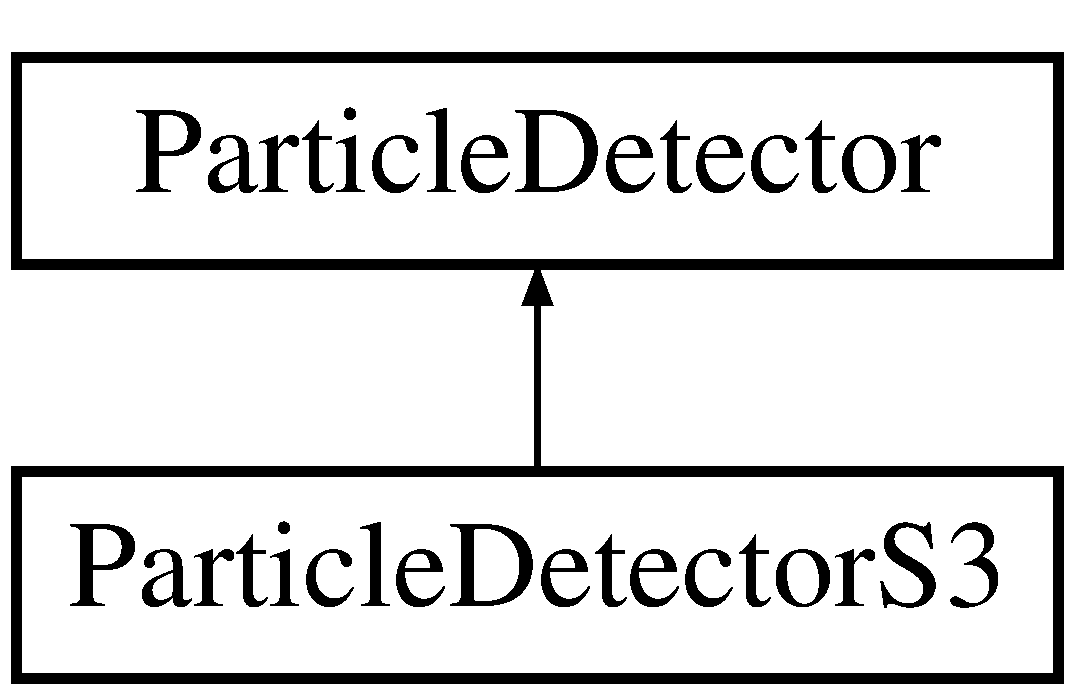
\includegraphics[height=2.000000cm]{classParticleDetector}
\end{center}
\end{figure}
\subsection*{Public Member Functions}
\begin{DoxyCompactItemize}
\item 
\hyperlink{classParticleDetector_ae4e67f0c8345fdc41aae3773b7207c32}{Particle\-Detector} (const \hyperlink{classParticleDetector}{Particle\-Detector} \&d)
\item 
\hyperlink{classParticleDetector}{Particle\-Detector} \& \hyperlink{classParticleDetector_aa0f3176c3ce050c7922631d14e4917b4}{operator=} (const \hyperlink{classParticleDetector}{Particle\-Detector} \&d)
\item 
virtual double \hyperlink{classParticleDetector_aaa0f7a2570187065fa058686fc5a8d47}{Get\-Efficiency\-Theta} (double)
\item 
virtual double \hyperlink{classParticleDetector_a67d7e51f3c565dd6cff3ff0225bd6572}{Get\-Theta\-Min} ()
\item 
virtual double \hyperlink{classParticleDetector_ad0380f4df4bbbaf307b4b475b337dd5b}{Get\-Theta\-Max} ()
\item 
virtual T\-H1\-F $\ast$ \hyperlink{classParticleDetector_aee088d19449faa1a4658a25f3e9a8491}{Get\-Theta\-Efficiency\-Hist} () const 
\item 
virtual T\-H2\-F $\ast$ \hyperlink{classParticleDetector_a35f50afc4ffafcf9a9ff86e06cb5fa30}{Get\-Theta\-Phi\-Map} () const 
\item 
virtual void \hyperlink{classParticleDetector_a8f27064544d26812431e508fefdf4945}{Write\-Particle\-Detector} (const char $\ast$filename, const char $\ast$opt=\char`\"{}U\-P\-D\-A\-T\-E\char`\"{})
\end{DoxyCompactItemize}
\subsection*{Protected Attributes}
\begin{DoxyCompactItemize}
\item 
T\-H2\-F $\ast$ \hyperlink{classParticleDetector_a23704fdd3fd36c821136ad14b89f8f4a}{h\-Theta\-Phi}
\item 
T\-H1\-F $\ast$ \hyperlink{classParticleDetector_a246ea62a664366cf8f05e870658bae09}{h\-Theta\-Eff}
\item 
bool \hyperlink{classParticleDetector_a52a6f3a2af63e5d5b8cd61b53a47e944}{set\-Flag}
\end{DoxyCompactItemize}


\subsection{Detailed Description}
Generic class to defined particle detection efficiencies in theta and phi for corrections to the integrated yields. 

Definition at line 18 of file Particle\-Detector.\-h.



\subsection{Constructor \& Destructor Documentation}
\hypertarget{classParticleDetector_ae4e67f0c8345fdc41aae3773b7207c32}{\index{Particle\-Detector@{Particle\-Detector}!Particle\-Detector@{Particle\-Detector}}
\index{Particle\-Detector@{Particle\-Detector}!ParticleDetector@{Particle\-Detector}}
\subsubsection[{Particle\-Detector}]{\setlength{\rightskip}{0pt plus 5cm}Particle\-Detector\-::\-Particle\-Detector (
\begin{DoxyParamCaption}
\item[{const {\bf Particle\-Detector} \&}]{d}
\end{DoxyParamCaption}
)}}\label{classParticleDetector_ae4e67f0c8345fdc41aae3773b7207c32}
Copy constructor 

Definition at line 3 of file Particle\-Detector.\-cxx.



\subsection{Member Function Documentation}
\hypertarget{classParticleDetector_aaa0f7a2570187065fa058686fc5a8d47}{\index{Particle\-Detector@{Particle\-Detector}!Get\-Efficiency\-Theta@{Get\-Efficiency\-Theta}}
\index{Get\-Efficiency\-Theta@{Get\-Efficiency\-Theta}!ParticleDetector@{Particle\-Detector}}
\subsubsection[{Get\-Efficiency\-Theta}]{\setlength{\rightskip}{0pt plus 5cm}double Particle\-Detector\-::\-Get\-Efficiency\-Theta (
\begin{DoxyParamCaption}
\item[{double}]{t}
\end{DoxyParamCaption}
)\hspace{0.3cm}{\ttfamily [virtual]}}}\label{classParticleDetector_aaa0f7a2570187065fa058686fc5a8d47}
Get the particle detection efficiency for a given thete (lab frame) 

Definition at line 20 of file Particle\-Detector.\-cxx.

\hypertarget{classParticleDetector_aee088d19449faa1a4658a25f3e9a8491}{\index{Particle\-Detector@{Particle\-Detector}!Get\-Theta\-Efficiency\-Hist@{Get\-Theta\-Efficiency\-Hist}}
\index{Get\-Theta\-Efficiency\-Hist@{Get\-Theta\-Efficiency\-Hist}!ParticleDetector@{Particle\-Detector}}
\subsubsection[{Get\-Theta\-Efficiency\-Hist}]{\setlength{\rightskip}{0pt plus 5cm}virtual T\-H1\-F$\ast$ Particle\-Detector\-::\-Get\-Theta\-Efficiency\-Hist (
\begin{DoxyParamCaption}
{}
\end{DoxyParamCaption}
) const\hspace{0.3cm}{\ttfamily [inline]}, {\ttfamily [virtual]}}}\label{classParticleDetector_aee088d19449faa1a4658a25f3e9a8491}
Return the 1\-D histogram, defining detection efficiency in theta 

Definition at line 31 of file Particle\-Detector.\-h.

\hypertarget{classParticleDetector_ad0380f4df4bbbaf307b4b475b337dd5b}{\index{Particle\-Detector@{Particle\-Detector}!Get\-Theta\-Max@{Get\-Theta\-Max}}
\index{Get\-Theta\-Max@{Get\-Theta\-Max}!ParticleDetector@{Particle\-Detector}}
\subsubsection[{Get\-Theta\-Max}]{\setlength{\rightskip}{0pt plus 5cm}double Particle\-Detector\-::\-Get\-Theta\-Max (
\begin{DoxyParamCaption}
{}
\end{DoxyParamCaption}
)\hspace{0.3cm}{\ttfamily [virtual]}}}\label{classParticleDetector_ad0380f4df4bbbaf307b4b475b337dd5b}
Find the maximum theta covered by the detector. For use to define the integration range. 

Definition at line 46 of file Particle\-Detector.\-cxx.

\hypertarget{classParticleDetector_a67d7e51f3c565dd6cff3ff0225bd6572}{\index{Particle\-Detector@{Particle\-Detector}!Get\-Theta\-Min@{Get\-Theta\-Min}}
\index{Get\-Theta\-Min@{Get\-Theta\-Min}!ParticleDetector@{Particle\-Detector}}
\subsubsection[{Get\-Theta\-Min}]{\setlength{\rightskip}{0pt plus 5cm}double Particle\-Detector\-::\-Get\-Theta\-Min (
\begin{DoxyParamCaption}
{}
\end{DoxyParamCaption}
)\hspace{0.3cm}{\ttfamily [virtual]}}}\label{classParticleDetector_a67d7e51f3c565dd6cff3ff0225bd6572}
Find the minimum theta covered by the detector. For use to define the integration range. 

Definition at line 33 of file Particle\-Detector.\-cxx.

\hypertarget{classParticleDetector_a35f50afc4ffafcf9a9ff86e06cb5fa30}{\index{Particle\-Detector@{Particle\-Detector}!Get\-Theta\-Phi\-Map@{Get\-Theta\-Phi\-Map}}
\index{Get\-Theta\-Phi\-Map@{Get\-Theta\-Phi\-Map}!ParticleDetector@{Particle\-Detector}}
\subsubsection[{Get\-Theta\-Phi\-Map}]{\setlength{\rightskip}{0pt plus 5cm}virtual T\-H2\-F$\ast$ Particle\-Detector\-::\-Get\-Theta\-Phi\-Map (
\begin{DoxyParamCaption}
{}
\end{DoxyParamCaption}
) const\hspace{0.3cm}{\ttfamily [inline]}, {\ttfamily [virtual]}}}\label{classParticleDetector_a35f50afc4ffafcf9a9ff86e06cb5fa30}
Return the 2\-D histogram, defining detection efficiency in theta and phi 

Definition at line 32 of file Particle\-Detector.\-h.

\hypertarget{classParticleDetector_aa0f3176c3ce050c7922631d14e4917b4}{\index{Particle\-Detector@{Particle\-Detector}!operator=@{operator=}}
\index{operator=@{operator=}!ParticleDetector@{Particle\-Detector}}
\subsubsection[{operator=}]{\setlength{\rightskip}{0pt plus 5cm}{\bf Particle\-Detector} \& Particle\-Detector\-::operator= (
\begin{DoxyParamCaption}
\item[{const {\bf Particle\-Detector} \&}]{d}
\end{DoxyParamCaption}
)}}\label{classParticleDetector_aa0f3176c3ce050c7922631d14e4917b4}
Assignment operator 

Definition at line 10 of file Particle\-Detector.\-cxx.

\hypertarget{classParticleDetector_a8f27064544d26812431e508fefdf4945}{\index{Particle\-Detector@{Particle\-Detector}!Write\-Particle\-Detector@{Write\-Particle\-Detector}}
\index{Write\-Particle\-Detector@{Write\-Particle\-Detector}!ParticleDetector@{Particle\-Detector}}
\subsubsection[{Write\-Particle\-Detector}]{\setlength{\rightskip}{0pt plus 5cm}void Particle\-Detector\-::\-Write\-Particle\-Detector (
\begin{DoxyParamCaption}
\item[{const char $\ast$}]{filename, }
\item[{const char $\ast$}]{opt = {\ttfamily \char`\"{}UPDATE\char`\"{}}}
\end{DoxyParamCaption}
)\hspace{0.3cm}{\ttfamily [virtual]}}}\label{classParticleDetector_a8f27064544d26812431e508fefdf4945}
Write the particle detection efficiencies to file, filename, with options, opt 

Definition at line 60 of file Particle\-Detector.\-cxx.



\subsection{Field Documentation}
\hypertarget{classParticleDetector_a246ea62a664366cf8f05e870658bae09}{\index{Particle\-Detector@{Particle\-Detector}!h\-Theta\-Eff@{h\-Theta\-Eff}}
\index{h\-Theta\-Eff@{h\-Theta\-Eff}!ParticleDetector@{Particle\-Detector}}
\subsubsection[{h\-Theta\-Eff}]{\setlength{\rightskip}{0pt plus 5cm}T\-H1\-F$\ast$ Particle\-Detector\-::h\-Theta\-Eff\hspace{0.3cm}{\ttfamily [protected]}}}\label{classParticleDetector_a246ea62a664366cf8f05e870658bae09}
Histogram defining particle detection efficiency in theta 

Definition at line 39 of file Particle\-Detector.\-h.

\hypertarget{classParticleDetector_a23704fdd3fd36c821136ad14b89f8f4a}{\index{Particle\-Detector@{Particle\-Detector}!h\-Theta\-Phi@{h\-Theta\-Phi}}
\index{h\-Theta\-Phi@{h\-Theta\-Phi}!ParticleDetector@{Particle\-Detector}}
\subsubsection[{h\-Theta\-Phi}]{\setlength{\rightskip}{0pt plus 5cm}T\-H2\-F$\ast$ Particle\-Detector\-::h\-Theta\-Phi\hspace{0.3cm}{\ttfamily [protected]}}}\label{classParticleDetector_a23704fdd3fd36c821136ad14b89f8f4a}
Histogram defining particle detection efficiency in theta and phi 

Definition at line 38 of file Particle\-Detector.\-h.

\hypertarget{classParticleDetector_a52a6f3a2af63e5d5b8cd61b53a47e944}{\index{Particle\-Detector@{Particle\-Detector}!set\-Flag@{set\-Flag}}
\index{set\-Flag@{set\-Flag}!ParticleDetector@{Particle\-Detector}}
\subsubsection[{set\-Flag}]{\setlength{\rightskip}{0pt plus 5cm}bool Particle\-Detector\-::set\-Flag\hspace{0.3cm}{\ttfamily [protected]}}}\label{classParticleDetector_a52a6f3a2af63e5d5b8cd61b53a47e944}
Indicates whether the efficiency maps have been defined 

Definition at line 40 of file Particle\-Detector.\-h.



The documentation for this class was generated from the following files\-:\begin{DoxyCompactItemize}
\item 
Particle\-Detector.\-h\item 
Particle\-Detector.\-cxx\end{DoxyCompactItemize}

\hypertarget{classParticleDetectorS3}{\section{Particle\-Detector\-S3 Class Reference}
\label{classParticleDetectorS3}\index{Particle\-Detector\-S3@{Particle\-Detector\-S3}}
}


Example class inheriting from the \hyperlink{classParticleDetector}{Particle\-Detector} class to define coverage based on an S3 detector.  




{\ttfamily \#include $<$Particle\-Detector\-S3.\-h$>$}

Inheritance diagram for Particle\-Detector\-S3\-:\begin{figure}[H]
\begin{center}
\leavevmode
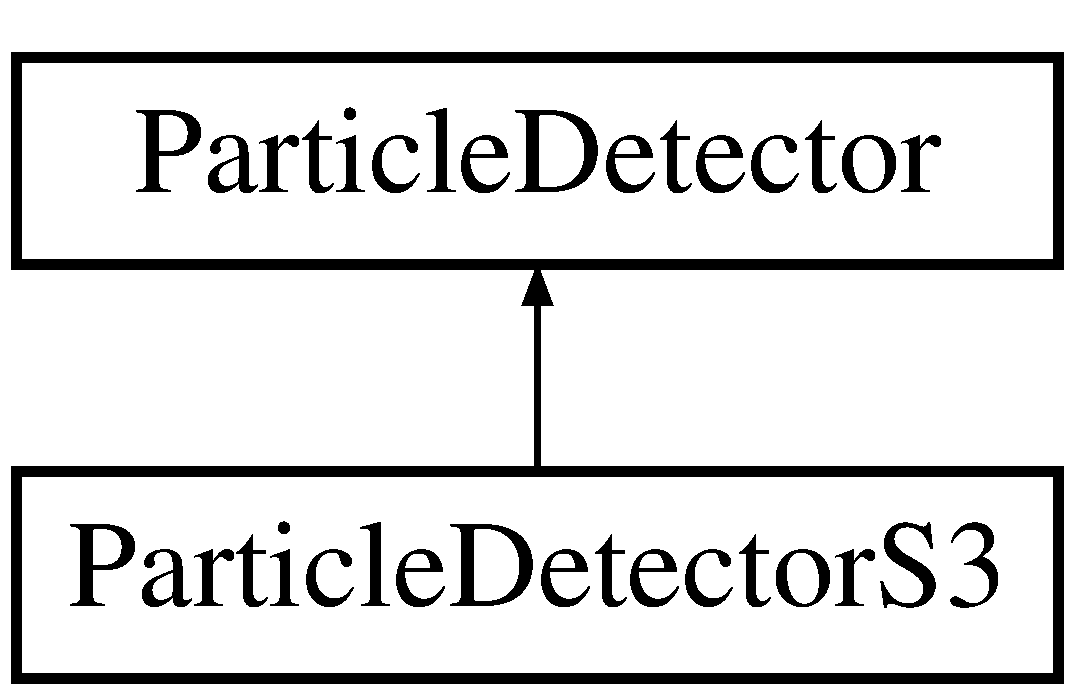
\includegraphics[height=2.000000cm]{classParticleDetectorS3}
\end{center}
\end{figure}
\subsection*{Public Member Functions}
\begin{DoxyCompactItemize}
\item 
\hyperlink{classParticleDetectorS3_a0da9b3baef00144759ca90a177e69cdc}{Particle\-Detector\-S3} (T\-Graph2\-D $\ast$, T\-Graph $\ast$)
\item 
\hypertarget{classParticleDetectorS3_a002873e132856865a40151e976974ad6}{{\bfseries Particle\-Detector\-S3} (int id, double z, double x\-\_\-off, double y\-\_\-off, int ring\-\_\-in, int ring\-\_\-out, double tmin=0, double tmax=180)}\label{classParticleDetectorS3_a002873e132856865a40151e976974ad6}

\end{DoxyCompactItemize}
\subsection*{Additional Inherited Members}


\subsection{Detailed Description}
Example class inheriting from the \hyperlink{classParticleDetector}{Particle\-Detector} class to define coverage based on an S3 detector. 

Definition at line 18 of file Particle\-Detector\-S3.\-h.



\subsection{Constructor \& Destructor Documentation}
\hypertarget{classParticleDetectorS3_a0da9b3baef00144759ca90a177e69cdc}{\index{Particle\-Detector\-S3@{Particle\-Detector\-S3}!Particle\-Detector\-S3@{Particle\-Detector\-S3}}
\index{Particle\-Detector\-S3@{Particle\-Detector\-S3}!ParticleDetectorS3@{Particle\-Detector\-S3}}
\subsubsection[{Particle\-Detector\-S3}]{\setlength{\rightskip}{0pt plus 5cm}Particle\-Detector\-S3\-::\-Particle\-Detector\-S3 (
\begin{DoxyParamCaption}
\item[{T\-Graph2\-D $\ast$}]{g2, }
\item[{T\-Graph $\ast$}]{g}
\end{DoxyParamCaption}
)}}\label{classParticleDetectorS3_a0da9b3baef00144759ca90a177e69cdc}
Define an S3 detector (or subset thereof) \par
id -\/ define the experiment index, for use in naming conventions of histograms \par
z -\/ the offset in z of the detector from the target position \par
x\-\_\-off -\/ the offset (from the beam axis) of the S3 detector in the x-\/direction \par
y\-\_\-off -\/ the offset (from the beam axis) of the S3 detector in the y-\/direction \par
ring\-\_\-in -\/ the innermost ring of the S3 in the experimental range \par
ring\-\_\-out -\/ the outermost ring of the S3 in this experimental range \par
tmin \& tmax -\/ define the maximum and minimum theta values in the efficiency histograms, this must cover a larger range than the detector 

Definition at line 3 of file Particle\-Detector\-S3.\-cxx.



The documentation for this class was generated from the following files\-:\begin{DoxyCompactItemize}
\item 
Particle\-Detector\-S3.\-h\item 
Particle\-Detector\-S3.\-cxx\end{DoxyCompactItemize}

\hypertarget{classPlotting}{\section{Plotting Class Reference}
\label{classPlotting}\index{Plotting@{Plotting}}
}
\subsection*{Static Public Member Functions}
\begin{DoxyCompactItemize}
\item 
\hypertarget{classPlotting_a7ba1f8e17589c29158908722127db4b2}{static T\-Graph $\ast$ {\bfseries Co\-M\-D\-Sig\-D\-Omega} (\hyperlink{classNucleus}{Nucleus} $\ast$, \hyperlink{classReaction}{Reaction} $\ast$, double, double, int, int n\-State=1, bool Proj\-Ex=true)}\label{classPlotting_a7ba1f8e17589c29158908722127db4b2}

\item 
\hypertarget{classPlotting_aec85a236379d09d6e6c00f8945faf0cb}{static T\-Graph $\ast$ {\bfseries Lab\-D\-Sig\-D\-Omega} (\hyperlink{classNucleus}{Nucleus} $\ast$, \hyperlink{classReaction}{Reaction} $\ast$, double, double, int, int n\-State=1, bool Proj\-Ex=true)}\label{classPlotting_aec85a236379d09d6e6c00f8945faf0cb}

\item 
\hypertarget{classPlotting_afd3c8e6c3a6e00d181e738047be7161a}{static T\-Graph $\ast$ {\bfseries Lab\-Sigma} (\hyperlink{classNucleus}{Nucleus} $\ast$, \hyperlink{classReaction}{Reaction} $\ast$, double, double, int, int n\-State=1, bool Proj\-Ex=true)}\label{classPlotting_afd3c8e6c3a6e00d181e738047be7161a}

\item 
\hypertarget{classPlotting_ae9766fb9575c6a914f1984440f829587}{static T\-Graph $\ast$ {\bfseries Co\-M\-Probability} (\hyperlink{classNucleus}{Nucleus} $\ast$, \hyperlink{classReaction}{Reaction} $\ast$, double, double, int, int n\-State=1, bool Proj\-Ex=true)}\label{classPlotting_ae9766fb9575c6a914f1984440f829587}

\item 
\hypertarget{classPlotting_a7f81dd921364ea2e0f0552f1ed45bfc1}{static T\-Graph $\ast$ {\bfseries Lab\-Probability} (\hyperlink{classNucleus}{Nucleus} $\ast$, \hyperlink{classReaction}{Reaction} $\ast$, double, double, int, int n\-State=1, bool Proj\-Ex=true)}\label{classPlotting_a7f81dd921364ea2e0f0552f1ed45bfc1}

\item 
\hypertarget{classPlotting_ab42f057b4c409a9066e21ff8aac1275f}{static T\-Graph $\ast$ {\bfseries Excitation\-Track} (\hyperlink{classNucleus}{Nucleus} $\ast$, \hyperlink{classReaction}{Reaction} $\ast$, double, double, int n\-State=1, bool Proj\-Ex=true)}\label{classPlotting_ab42f057b4c409a9066e21ff8aac1275f}

\item 
\hypertarget{classPlotting_ad5ca78a0dbe4ad43259c6c5dcd50614a}{static T\-Graph $\ast$ {\bfseries Differential\-Excitation\-Track} (\hyperlink{classNucleus}{Nucleus} $\ast$, \hyperlink{classReaction}{Reaction} $\ast$, double, double, int n\-State=1, bool Proj\-Ex=true)}\label{classPlotting_ad5ca78a0dbe4ad43259c6c5dcd50614a}

\end{DoxyCompactItemize}


\subsection{Detailed Description}


Definition at line 10 of file Plotting.\-h.



The documentation for this class was generated from the following files\-:\begin{DoxyCompactItemize}
\item 
Plotting.\-h\item 
Plotting.\-cxx\end{DoxyCompactItemize}

\hypertarget{classPointCoulEx}{\section{Point\-Coul\-Ex Class Reference}
\label{classPointCoulEx}\index{Point\-Coul\-Ex@{Point\-Coul\-Ex}}
}


Calculate point Coulomb excitation amplitudes and associated statistical tensors.  




{\ttfamily \#include $<$Point\-Coul\-Ex.\-h$>$}

\subsection*{Public Member Functions}
\begin{DoxyCompactItemize}
\item 
\hyperlink{classPointCoulEx_a9246400fa6440b3628cdb3010e733f3c}{Point\-Coul\-Ex} (\hyperlink{classNucleus}{Nucleus} $\ast$, \hyperlink{classReaction}{Reaction} $\ast$)
\item 
\hyperlink{classPointCoulEx_ae304214fe53d62d39b1413bf179bd0bd}{Point\-Coul\-Ex} (const \hyperlink{classPointCoulEx}{Point\-Coul\-Ex} \&p)
\item 
\hyperlink{classPointCoulEx}{Point\-Coul\-Ex} \& \hyperlink{classPointCoulEx_ac812c4e40026a7becd63c583b63aaf43}{operator=} (const \hyperlink{classPointCoulEx}{Point\-Coul\-Ex} \&p)
\item 
T\-Vector\-D \hyperlink{classPointCoulEx_ae3636eacee3ab0f37d0b8c927d779387}{Point\-Probabilities} (double)
\item 
void \hyperlink{classPointCoulEx_a350a143e891ac63bb7088559a20081dc}{Calculate\-Point\-Probabilities} (double)
\item 
T\-Vector\-D \hyperlink{classPointCoulEx_a7af998470e383eb70c74c3dae33a85b6}{Get\-Probabilities\-Vector} () const 
\item 
void \hyperlink{classPointCoulEx_a8e109cc21be7be0abb69fb561bab4dcf}{Set\-Nucleus} (\hyperlink{classNucleus}{Nucleus} $\ast$nucl)
\item 
void \hyperlink{classPointCoulEx_a2b3413601d938ca86e6ccf0aa8e09f37}{Set\-Reaction} (\hyperlink{classReaction}{Reaction} $\ast$reac)
\item 
void \hyperlink{classPointCoulEx_aea871d21af150c2ca49c95be891bc717}{Set\-Projectile\-Excitation} (bool b=true)
\item 
\hypertarget{classPointCoulEx_a547911f31b59fb1e3d5bb9492e097422}{void {\bfseries Set\-Target\-Detection} (bool b=true)}\label{classPointCoulEx_a547911f31b59fb1e3d5bb9492e097422}

\item 
\hyperlink{classNucleus}{Nucleus} $\ast$ \hyperlink{classPointCoulEx_a0190b4e42074c4198e80f3403d25b14e}{Get\-Nucleus} ()
\item 
\hyperlink{classReaction}{Reaction} $\ast$ \hyperlink{classPointCoulEx_a4369d10a2ab275ffd79800f4b2946345}{Get\-Reaction} ()
\item 
void \hyperlink{classPointCoulEx_afd63f7b47fc6fb5f49906911cb212b38}{Set\-Verbose} (bool b=true)
\item 
void \hyperlink{classPointCoulEx_a1bfa7f85286b1da3c4f0622ee35d0087}{Prepare\-Connections} ()
\item 
void \hyperlink{classPointCoulEx_a80b13791f6bfd42e2ab75895e1617ee3}{Set\-Accuracy} (double acc)
\item 
void \hyperlink{classPointCoulEx_aa6006da1bca6a0bc677c4fb23ba38dcd}{Print} ()
\item 
void \hyperlink{classPointCoulEx_a409e44329209abf7d2e4bfc794b2bb1e}{Write\-Details\-To\-File} (const char $\ast$outfilename=\char`\"{}Coul\-Ex\-\_\-\-Calculation\-Details.\-txt\char`\"{})
\item 
void \hyperlink{classPointCoulEx_aa7fa9cd089c327c59eef9ec4e7f46e0e}{Write\-Matrix} (std\-::ofstream \&, T\-Matrix\-D)
\item 
void \hyperlink{classPointCoulEx_a8786b398bd1d6d790f203c87cef957cc}{Write\-Connections} (std\-::ofstream \&)
\item 
T\-Matrix\-D \hyperlink{classPointCoulEx_aa53de9a5ae2bd43ef3b3287cffaccc67}{Get\-Final\-Real\-Amplitude} () const 
\item 
T\-Matrix\-D \hyperlink{classPointCoulEx_a13792d4d252f16cd4c1bb881757dea30}{Get\-Final\-Imag\-Amplitude} () const 
\item 
void \hyperlink{classPointCoulEx_a276ea0591ad200fbd40a53ac80c61634}{Calculate\-Tensors} ()
\item 
\hyperlink{classStatisticalTensor}{Statistical\-Tensor} \hyperlink{classPointCoulEx_a08232c7aba802b4820dc3859bf183a2e}{Get\-Tensors} ()
\item 
\hyperlink{classStatisticalTensor}{Statistical\-Tensor} \hyperlink{classPointCoulEx_af4dca3329edc2696b088140eceef5bda}{Get\-Tensors\-B} ()
\item 
void \hyperlink{classPointCoulEx_aa03b7b60a372846b772659ff1b16c246}{Track\-Reaction} (bool b=true)
\item 
bool \hyperlink{classPointCoulEx_a65c1db61988871c76583e54d52b721ec}{Tracking} () const 
\item 
double \hyperlink{classPointCoulEx_a1e1d91eff35bba0a4ed36610a8644638}{Get\-Epsilon} () const 
\item 
std\-::vector$<$ double $>$ \hyperlink{classPointCoulEx_a2f447409074ae1105d54bcdf4aaad3fd}{Get\-Omega} () const 
\item 
std\-::vector$<$ std\-::vector\\*
$<$ double $>$ $>$ \hyperlink{classPointCoulEx_a5324fc5b5d28c980ae0919bb7de6bb02}{Get\-Probability\-Track} () const 
\item 
double \hyperlink{classPointCoulEx_a593fc5d2387da403ffaa6ceb12527ba0}{Get\-Theta} () const 
\end{DoxyCompactItemize}


\subsection{Detailed Description}
Calculate point Coulomb excitation amplitudes and associated statistical tensors. 

This class does the majority of the heavy lifting, calculating the Coulomb-\/excitation amplitudes and probabilities. The syntax borrows heavily from both G\-O\-S\-I\-A and C\-L\-X methods, but is organized rather differently.

\hyperlink{classConnection}{Connection} information, rather than being stored in a number of matrices (as in C\-L\-X and G\-O\-S\-I\-A) is collected in a vector of \hyperlink{classSubstate}{Substate} objects.

The program then cycles through these substates during amplitude calculation.

The numerical integration of the coupled-\/differential equations is performed using the C\-L\-X method\-:\par
A Runge-\/\-Kutta algorithm is used to determine four initial points, before the Adams-\/\-Moulton method is employed. This differs from G\-O\-S\-I\-A, in which a pertubative technique is used to determine initial points. In practice, differences between methods are insignificant.

The class also calculates the statistical tensors in both the reaction frame and the laboratory frame and stores them in \hyperlink{classStatisticalTensor}{Statistical\-Tensor} objects (f\-Tensors and f\-Tensors\-B). 

Definition at line 53 of file Point\-Coul\-Ex.\-h.



\subsection{Constructor \& Destructor Documentation}
\hypertarget{classPointCoulEx_a9246400fa6440b3628cdb3010e733f3c}{\index{Point\-Coul\-Ex@{Point\-Coul\-Ex}!Point\-Coul\-Ex@{Point\-Coul\-Ex}}
\index{Point\-Coul\-Ex@{Point\-Coul\-Ex}!PointCoulEx@{Point\-Coul\-Ex}}
\subsubsection[{Point\-Coul\-Ex}]{\setlength{\rightskip}{0pt plus 5cm}Point\-Coul\-Ex\-::\-Point\-Coul\-Ex (
\begin{DoxyParamCaption}
\item[{{\bf Nucleus} $\ast$}]{nuc, }
\item[{{\bf Reaction} $\ast$}]{reac}
\end{DoxyParamCaption}
)}}\label{classPointCoulEx_a9246400fa6440b3628cdb3010e733f3c}
Constructor, passing \hyperlink{classNucleus}{Nucleus} and Reactions immediately 

Definition at line 20 of file Point\-Coul\-Ex.\-cxx.

\hypertarget{classPointCoulEx_ae304214fe53d62d39b1413bf179bd0bd}{\index{Point\-Coul\-Ex@{Point\-Coul\-Ex}!Point\-Coul\-Ex@{Point\-Coul\-Ex}}
\index{Point\-Coul\-Ex@{Point\-Coul\-Ex}!PointCoulEx@{Point\-Coul\-Ex}}
\subsubsection[{Point\-Coul\-Ex}]{\setlength{\rightskip}{0pt plus 5cm}Point\-Coul\-Ex\-::\-Point\-Coul\-Ex (
\begin{DoxyParamCaption}
\item[{const {\bf Point\-Coul\-Ex} \&}]{p}
\end{DoxyParamCaption}
)}}\label{classPointCoulEx_ae304214fe53d62d39b1413bf179bd0bd}
Copy constructor 

Definition at line 44 of file Point\-Coul\-Ex.\-cxx.



\subsection{Member Function Documentation}
\hypertarget{classPointCoulEx_a350a143e891ac63bb7088559a20081dc}{\index{Point\-Coul\-Ex@{Point\-Coul\-Ex}!Calculate\-Point\-Probabilities@{Calculate\-Point\-Probabilities}}
\index{Calculate\-Point\-Probabilities@{Calculate\-Point\-Probabilities}!PointCoulEx@{Point\-Coul\-Ex}}
\subsubsection[{Calculate\-Point\-Probabilities}]{\setlength{\rightskip}{0pt plus 5cm}void Point\-Coul\-Ex\-::\-Calculate\-Point\-Probabilities (
\begin{DoxyParamCaption}
\item[{double}]{theta}
\end{DoxyParamCaption}
)}}\label{classPointCoulEx_a350a143e891ac63bb7088559a20081dc}
Calculate the point probabilities 

Definition at line 368 of file Point\-Coul\-Ex.\-cxx.

\hypertarget{classPointCoulEx_a276ea0591ad200fbd40a53ac80c61634}{\index{Point\-Coul\-Ex@{Point\-Coul\-Ex}!Calculate\-Tensors@{Calculate\-Tensors}}
\index{Calculate\-Tensors@{Calculate\-Tensors}!PointCoulEx@{Point\-Coul\-Ex}}
\subsubsection[{Calculate\-Tensors}]{\setlength{\rightskip}{0pt plus 5cm}void Point\-Coul\-Ex\-::\-Calculate\-Tensors (
\begin{DoxyParamCaption}
{}
\end{DoxyParamCaption}
)}}\label{classPointCoulEx_a276ea0591ad200fbd40a53ac80c61634}
Calculate the statistical tensors based on the final amplitudes 

Definition at line 1003 of file Point\-Coul\-Ex.\-cxx.

\hypertarget{classPointCoulEx_a1e1d91eff35bba0a4ed36610a8644638}{\index{Point\-Coul\-Ex@{Point\-Coul\-Ex}!Get\-Epsilon@{Get\-Epsilon}}
\index{Get\-Epsilon@{Get\-Epsilon}!PointCoulEx@{Point\-Coul\-Ex}}
\subsubsection[{Get\-Epsilon}]{\setlength{\rightskip}{0pt plus 5cm}double Point\-Coul\-Ex\-::\-Get\-Epsilon (
\begin{DoxyParamCaption}
{}
\end{DoxyParamCaption}
) const\hspace{0.3cm}{\ttfamily [inline]}}}\label{classPointCoulEx_a1e1d91eff35bba0a4ed36610a8644638}
Return the epsilon (theta proxy) of the reaction 

Definition at line 104 of file Point\-Coul\-Ex.\-h.

\hypertarget{classPointCoulEx_a13792d4d252f16cd4c1bb881757dea30}{\index{Point\-Coul\-Ex@{Point\-Coul\-Ex}!Get\-Final\-Imag\-Amplitude@{Get\-Final\-Imag\-Amplitude}}
\index{Get\-Final\-Imag\-Amplitude@{Get\-Final\-Imag\-Amplitude}!PointCoulEx@{Point\-Coul\-Ex}}
\subsubsection[{Get\-Final\-Imag\-Amplitude}]{\setlength{\rightskip}{0pt plus 5cm}T\-Matrix\-D Point\-Coul\-Ex\-::\-Get\-Final\-Imag\-Amplitude (
\begin{DoxyParamCaption}
{}
\end{DoxyParamCaption}
) const\hspace{0.3cm}{\ttfamily [inline]}}}\label{classPointCoulEx_a13792d4d252f16cd4c1bb881757dea30}
Return the imaginary components of the final amplitudes 

Definition at line 95 of file Point\-Coul\-Ex.\-h.

\hypertarget{classPointCoulEx_aa53de9a5ae2bd43ef3b3287cffaccc67}{\index{Point\-Coul\-Ex@{Point\-Coul\-Ex}!Get\-Final\-Real\-Amplitude@{Get\-Final\-Real\-Amplitude}}
\index{Get\-Final\-Real\-Amplitude@{Get\-Final\-Real\-Amplitude}!PointCoulEx@{Point\-Coul\-Ex}}
\subsubsection[{Get\-Final\-Real\-Amplitude}]{\setlength{\rightskip}{0pt plus 5cm}T\-Matrix\-D Point\-Coul\-Ex\-::\-Get\-Final\-Real\-Amplitude (
\begin{DoxyParamCaption}
{}
\end{DoxyParamCaption}
) const\hspace{0.3cm}{\ttfamily [inline]}}}\label{classPointCoulEx_aa53de9a5ae2bd43ef3b3287cffaccc67}
Return the real components of the final amplitudes 

Definition at line 94 of file Point\-Coul\-Ex.\-h.

\hypertarget{classPointCoulEx_a0190b4e42074c4198e80f3403d25b14e}{\index{Point\-Coul\-Ex@{Point\-Coul\-Ex}!Get\-Nucleus@{Get\-Nucleus}}
\index{Get\-Nucleus@{Get\-Nucleus}!PointCoulEx@{Point\-Coul\-Ex}}
\subsubsection[{Get\-Nucleus}]{\setlength{\rightskip}{0pt plus 5cm}{\bf Nucleus}$\ast$ Point\-Coul\-Ex\-::\-Get\-Nucleus (
\begin{DoxyParamCaption}
{}
\end{DoxyParamCaption}
)\hspace{0.3cm}{\ttfamily [inline]}}}\label{classPointCoulEx_a0190b4e42074c4198e80f3403d25b14e}
Return the \hyperlink{classNucleus}{Nucleus} used in the calculation 

Definition at line 79 of file Point\-Coul\-Ex.\-h.

\hypertarget{classPointCoulEx_a2f447409074ae1105d54bcdf4aaad3fd}{\index{Point\-Coul\-Ex@{Point\-Coul\-Ex}!Get\-Omega@{Get\-Omega}}
\index{Get\-Omega@{Get\-Omega}!PointCoulEx@{Point\-Coul\-Ex}}
\subsubsection[{Get\-Omega}]{\setlength{\rightskip}{0pt plus 5cm}std\-::vector$<$double$>$ Point\-Coul\-Ex\-::\-Get\-Omega (
\begin{DoxyParamCaption}
{}
\end{DoxyParamCaption}
) const\hspace{0.3cm}{\ttfamily [inline]}}}\label{classPointCoulEx_a2f447409074ae1105d54bcdf4aaad3fd}
Return a vector of the omega (time proxy) values during the reaction 

Definition at line 105 of file Point\-Coul\-Ex.\-h.

\hypertarget{classPointCoulEx_a7af998470e383eb70c74c3dae33a85b6}{\index{Point\-Coul\-Ex@{Point\-Coul\-Ex}!Get\-Probabilities\-Vector@{Get\-Probabilities\-Vector}}
\index{Get\-Probabilities\-Vector@{Get\-Probabilities\-Vector}!PointCoulEx@{Point\-Coul\-Ex}}
\subsubsection[{Get\-Probabilities\-Vector}]{\setlength{\rightskip}{0pt plus 5cm}T\-Vector\-D Point\-Coul\-Ex\-::\-Get\-Probabilities\-Vector (
\begin{DoxyParamCaption}
{}
\end{DoxyParamCaption}
) const\hspace{0.3cm}{\ttfamily [inline]}}}\label{classPointCoulEx_a7af998470e383eb70c74c3dae33a85b6}
Returns previously calculated point probabilities 

Definition at line 67 of file Point\-Coul\-Ex.\-h.

\hypertarget{classPointCoulEx_a5324fc5b5d28c980ae0919bb7de6bb02}{\index{Point\-Coul\-Ex@{Point\-Coul\-Ex}!Get\-Probability\-Track@{Get\-Probability\-Track}}
\index{Get\-Probability\-Track@{Get\-Probability\-Track}!PointCoulEx@{Point\-Coul\-Ex}}
\subsubsection[{Get\-Probability\-Track}]{\setlength{\rightskip}{0pt plus 5cm}std\-::vector$<$std\-::vector$<$double$>$ $>$ Point\-Coul\-Ex\-::\-Get\-Probability\-Track (
\begin{DoxyParamCaption}
{}
\end{DoxyParamCaption}
) const\hspace{0.3cm}{\ttfamily [inline]}}}\label{classPointCoulEx_a5324fc5b5d28c980ae0919bb7de6bb02}
Return the probabilities, step-\/by-\/step, during the reaction 

Definition at line 106 of file Point\-Coul\-Ex.\-h.

\hypertarget{classPointCoulEx_a4369d10a2ab275ffd79800f4b2946345}{\index{Point\-Coul\-Ex@{Point\-Coul\-Ex}!Get\-Reaction@{Get\-Reaction}}
\index{Get\-Reaction@{Get\-Reaction}!PointCoulEx@{Point\-Coul\-Ex}}
\subsubsection[{Get\-Reaction}]{\setlength{\rightskip}{0pt plus 5cm}{\bf Reaction}$\ast$ Point\-Coul\-Ex\-::\-Get\-Reaction (
\begin{DoxyParamCaption}
{}
\end{DoxyParamCaption}
)\hspace{0.3cm}{\ttfamily [inline]}}}\label{classPointCoulEx_a4369d10a2ab275ffd79800f4b2946345}
Return the \hyperlink{classReaction}{Reaction} used in the calculation 

Definition at line 80 of file Point\-Coul\-Ex.\-h.

\hypertarget{classPointCoulEx_a08232c7aba802b4820dc3859bf183a2e}{\index{Point\-Coul\-Ex@{Point\-Coul\-Ex}!Get\-Tensors@{Get\-Tensors}}
\index{Get\-Tensors@{Get\-Tensors}!PointCoulEx@{Point\-Coul\-Ex}}
\subsubsection[{Get\-Tensors}]{\setlength{\rightskip}{0pt plus 5cm}{\bf Statistical\-Tensor} Point\-Coul\-Ex\-::\-Get\-Tensors (
\begin{DoxyParamCaption}
{}
\end{DoxyParamCaption}
)\hspace{0.3cm}{\ttfamily [inline]}}}\label{classPointCoulEx_a08232c7aba802b4820dc3859bf183a2e}
Return the calculated statistical tensors 

Definition at line 98 of file Point\-Coul\-Ex.\-h.

\hypertarget{classPointCoulEx_af4dca3329edc2696b088140eceef5bda}{\index{Point\-Coul\-Ex@{Point\-Coul\-Ex}!Get\-Tensors\-B@{Get\-Tensors\-B}}
\index{Get\-Tensors\-B@{Get\-Tensors\-B}!PointCoulEx@{Point\-Coul\-Ex}}
\subsubsection[{Get\-Tensors\-B}]{\setlength{\rightskip}{0pt plus 5cm}{\bf Statistical\-Tensor} Point\-Coul\-Ex\-::\-Get\-Tensors\-B (
\begin{DoxyParamCaption}
{}
\end{DoxyParamCaption}
)\hspace{0.3cm}{\ttfamily [inline]}}}\label{classPointCoulEx_af4dca3329edc2696b088140eceef5bda}
Return the calculated statistical tensors 

Definition at line 99 of file Point\-Coul\-Ex.\-h.

\hypertarget{classPointCoulEx_a593fc5d2387da403ffaa6ceb12527ba0}{\index{Point\-Coul\-Ex@{Point\-Coul\-Ex}!Get\-Theta@{Get\-Theta}}
\index{Get\-Theta@{Get\-Theta}!PointCoulEx@{Point\-Coul\-Ex}}
\subsubsection[{Get\-Theta}]{\setlength{\rightskip}{0pt plus 5cm}double Point\-Coul\-Ex\-::\-Get\-Theta (
\begin{DoxyParamCaption}
{}
\end{DoxyParamCaption}
) const\hspace{0.3cm}{\ttfamily [inline]}}}\label{classPointCoulEx_a593fc5d2387da403ffaa6ceb12527ba0}
Return the theta value 

Definition at line 108 of file Point\-Coul\-Ex.\-h.

\hypertarget{classPointCoulEx_ac812c4e40026a7becd63c583b63aaf43}{\index{Point\-Coul\-Ex@{Point\-Coul\-Ex}!operator=@{operator=}}
\index{operator=@{operator=}!PointCoulEx@{Point\-Coul\-Ex}}
\subsubsection[{operator=}]{\setlength{\rightskip}{0pt plus 5cm}{\bf Point\-Coul\-Ex} \& Point\-Coul\-Ex\-::operator= (
\begin{DoxyParamCaption}
\item[{const {\bf Point\-Coul\-Ex} \&}]{p}
\end{DoxyParamCaption}
)}}\label{classPointCoulEx_ac812c4e40026a7becd63c583b63aaf43}
Assignment operator 

Definition at line 97 of file Point\-Coul\-Ex.\-cxx.

\hypertarget{classPointCoulEx_ae3636eacee3ab0f37d0b8c927d779387}{\index{Point\-Coul\-Ex@{Point\-Coul\-Ex}!Point\-Probabilities@{Point\-Probabilities}}
\index{Point\-Probabilities@{Point\-Probabilities}!PointCoulEx@{Point\-Coul\-Ex}}
\subsubsection[{Point\-Probabilities}]{\setlength{\rightskip}{0pt plus 5cm}T\-Vector\-D Point\-Coul\-Ex\-::\-Point\-Probabilities (
\begin{DoxyParamCaption}
\item[{double}]{theta}
\end{DoxyParamCaption}
)}}\label{classPointCoulEx_ae3636eacee3ab0f37d0b8c927d779387}
Calculate the point probabilities and immediately pass them 

Definition at line 354 of file Point\-Coul\-Ex.\-cxx.

\hypertarget{classPointCoulEx_a1bfa7f85286b1da3c4f0622ee35d0087}{\index{Point\-Coul\-Ex@{Point\-Coul\-Ex}!Prepare\-Connections@{Prepare\-Connections}}
\index{Prepare\-Connections@{Prepare\-Connections}!PointCoulEx@{Point\-Coul\-Ex}}
\subsubsection[{Prepare\-Connections}]{\setlength{\rightskip}{0pt plus 5cm}void Point\-Coul\-Ex\-::\-Prepare\-Connections (
\begin{DoxyParamCaption}
{}
\end{DoxyParamCaption}
)}}\label{classPointCoulEx_a1bfa7f85286b1da3c4f0622ee35d0087}
Before performing the calculation, set up the connections between the substates 

Definition at line 163 of file Point\-Coul\-Ex.\-cxx.

\hypertarget{classPointCoulEx_aa6006da1bca6a0bc677c4fb23ba38dcd}{\index{Point\-Coul\-Ex@{Point\-Coul\-Ex}!Print@{Print}}
\index{Print@{Print}!PointCoulEx@{Point\-Coul\-Ex}}
\subsubsection[{Print}]{\setlength{\rightskip}{0pt plus 5cm}void Point\-Coul\-Ex\-::\-Print (
\begin{DoxyParamCaption}
{}
\end{DoxyParamCaption}
)}}\label{classPointCoulEx_aa6006da1bca6a0bc677c4fb23ba38dcd}
Simple print function 

Definition at line 1176 of file Point\-Coul\-Ex.\-cxx.

\hypertarget{classPointCoulEx_a80b13791f6bfd42e2ab75895e1617ee3}{\index{Point\-Coul\-Ex@{Point\-Coul\-Ex}!Set\-Accuracy@{Set\-Accuracy}}
\index{Set\-Accuracy@{Set\-Accuracy}!PointCoulEx@{Point\-Coul\-Ex}}
\subsubsection[{Set\-Accuracy}]{\setlength{\rightskip}{0pt plus 5cm}void Point\-Coul\-Ex\-::\-Set\-Accuracy (
\begin{DoxyParamCaption}
\item[{double}]{acc}
\end{DoxyParamCaption}
)\hspace{0.3cm}{\ttfamily [inline]}}}\label{classPointCoulEx_a80b13791f6bfd42e2ab75895e1617ee3}
Define the accuracy of the point calculation 

Definition at line 86 of file Point\-Coul\-Ex.\-h.

\hypertarget{classPointCoulEx_a8e109cc21be7be0abb69fb561bab4dcf}{\index{Point\-Coul\-Ex@{Point\-Coul\-Ex}!Set\-Nucleus@{Set\-Nucleus}}
\index{Set\-Nucleus@{Set\-Nucleus}!PointCoulEx@{Point\-Coul\-Ex}}
\subsubsection[{Set\-Nucleus}]{\setlength{\rightskip}{0pt plus 5cm}void Point\-Coul\-Ex\-::\-Set\-Nucleus (
\begin{DoxyParamCaption}
\item[{{\bf Nucleus} $\ast$}]{nucl}
\end{DoxyParamCaption}
)\hspace{0.3cm}{\ttfamily [inline]}}}\label{classPointCoulEx_a8e109cc21be7be0abb69fb561bab4dcf}
Define the \hyperlink{classNucleus}{Nucleus} to be used in the point calculation 

Definition at line 69 of file Point\-Coul\-Ex.\-h.

\hypertarget{classPointCoulEx_aea871d21af150c2ca49c95be891bc717}{\index{Point\-Coul\-Ex@{Point\-Coul\-Ex}!Set\-Projectile\-Excitation@{Set\-Projectile\-Excitation}}
\index{Set\-Projectile\-Excitation@{Set\-Projectile\-Excitation}!PointCoulEx@{Point\-Coul\-Ex}}
\subsubsection[{Set\-Projectile\-Excitation}]{\setlength{\rightskip}{0pt plus 5cm}void Point\-Coul\-Ex\-::\-Set\-Projectile\-Excitation (
\begin{DoxyParamCaption}
\item[{bool}]{b = {\ttfamily true}}
\end{DoxyParamCaption}
)\hspace{0.3cm}{\ttfamily [inline]}}}\label{classPointCoulEx_aea871d21af150c2ca49c95be891bc717}
Define whether projectile or target excitation is being calculated 

Definition at line 72 of file Point\-Coul\-Ex.\-h.

\hypertarget{classPointCoulEx_a2b3413601d938ca86e6ccf0aa8e09f37}{\index{Point\-Coul\-Ex@{Point\-Coul\-Ex}!Set\-Reaction@{Set\-Reaction}}
\index{Set\-Reaction@{Set\-Reaction}!PointCoulEx@{Point\-Coul\-Ex}}
\subsubsection[{Set\-Reaction}]{\setlength{\rightskip}{0pt plus 5cm}void Point\-Coul\-Ex\-::\-Set\-Reaction (
\begin{DoxyParamCaption}
\item[{{\bf Reaction} $\ast$}]{reac}
\end{DoxyParamCaption}
)\hspace{0.3cm}{\ttfamily [inline]}}}\label{classPointCoulEx_a2b3413601d938ca86e6ccf0aa8e09f37}
Define the \hyperlink{classReaction}{Reaction} kinematics for the point calculation 

Definition at line 70 of file Point\-Coul\-Ex.\-h.

\hypertarget{classPointCoulEx_afd63f7b47fc6fb5f49906911cb212b38}{\index{Point\-Coul\-Ex@{Point\-Coul\-Ex}!Set\-Verbose@{Set\-Verbose}}
\index{Set\-Verbose@{Set\-Verbose}!PointCoulEx@{Point\-Coul\-Ex}}
\subsubsection[{Set\-Verbose}]{\setlength{\rightskip}{0pt plus 5cm}void Point\-Coul\-Ex\-::\-Set\-Verbose (
\begin{DoxyParamCaption}
\item[{bool}]{b = {\ttfamily true}}
\end{DoxyParamCaption}
)\hspace{0.3cm}{\ttfamily [inline]}}}\label{classPointCoulEx_afd63f7b47fc6fb5f49906911cb212b38}
Define the verbocity of the calculation 

Definition at line 82 of file Point\-Coul\-Ex.\-h.

\hypertarget{classPointCoulEx_a65c1db61988871c76583e54d52b721ec}{\index{Point\-Coul\-Ex@{Point\-Coul\-Ex}!Tracking@{Tracking}}
\index{Tracking@{Tracking}!PointCoulEx@{Point\-Coul\-Ex}}
\subsubsection[{Tracking}]{\setlength{\rightskip}{0pt plus 5cm}bool Point\-Coul\-Ex\-::\-Tracking (
\begin{DoxyParamCaption}
{}
\end{DoxyParamCaption}
) const\hspace{0.3cm}{\ttfamily [inline]}}}\label{classPointCoulEx_a65c1db61988871c76583e54d52b721ec}
Is the reaction being tracker? 

Definition at line 102 of file Point\-Coul\-Ex.\-h.

\hypertarget{classPointCoulEx_aa03b7b60a372846b772659ff1b16c246}{\index{Point\-Coul\-Ex@{Point\-Coul\-Ex}!Track\-Reaction@{Track\-Reaction}}
\index{Track\-Reaction@{Track\-Reaction}!PointCoulEx@{Point\-Coul\-Ex}}
\subsubsection[{Track\-Reaction}]{\setlength{\rightskip}{0pt plus 5cm}void Point\-Coul\-Ex\-::\-Track\-Reaction (
\begin{DoxyParamCaption}
\item[{bool}]{b = {\ttfamily true}}
\end{DoxyParamCaption}
)\hspace{0.3cm}{\ttfamily [inline]}}}\label{classPointCoulEx_aa03b7b60a372846b772659ff1b16c246}
Track the reaction, step-\/by-\/step. Off by default. 

Definition at line 101 of file Point\-Coul\-Ex.\-h.

\hypertarget{classPointCoulEx_a8786b398bd1d6d790f203c87cef957cc}{\index{Point\-Coul\-Ex@{Point\-Coul\-Ex}!Write\-Connections@{Write\-Connections}}
\index{Write\-Connections@{Write\-Connections}!PointCoulEx@{Point\-Coul\-Ex}}
\subsubsection[{Write\-Connections}]{\setlength{\rightskip}{0pt plus 5cm}void Point\-Coul\-Ex\-::\-Write\-Connections (
\begin{DoxyParamCaption}
\item[{std\-::ofstream \&}]{outfile}
\end{DoxyParamCaption}
)}}\label{classPointCoulEx_a8786b398bd1d6d790f203c87cef957cc}
Write the connections between substates in a well formatted manner 

Definition at line 1340 of file Point\-Coul\-Ex.\-cxx.

\hypertarget{classPointCoulEx_a409e44329209abf7d2e4bfc794b2bb1e}{\index{Point\-Coul\-Ex@{Point\-Coul\-Ex}!Write\-Details\-To\-File@{Write\-Details\-To\-File}}
\index{Write\-Details\-To\-File@{Write\-Details\-To\-File}!PointCoulEx@{Point\-Coul\-Ex}}
\subsubsection[{Write\-Details\-To\-File}]{\setlength{\rightskip}{0pt plus 5cm}void Point\-Coul\-Ex\-::\-Write\-Details\-To\-File (
\begin{DoxyParamCaption}
\item[{const char $\ast$}]{outfilename = {\ttfamily \char`\"{}CoulEx\-\_\-CalculationDetails.txt\char`\"{}}}
\end{DoxyParamCaption}
)}}\label{classPointCoulEx_a409e44329209abf7d2e4bfc794b2bb1e}
Write the calculation details to a text file for debugging purposes 

Definition at line 1197 of file Point\-Coul\-Ex.\-cxx.

\hypertarget{classPointCoulEx_aa7fa9cd089c327c59eef9ec4e7f46e0e}{\index{Point\-Coul\-Ex@{Point\-Coul\-Ex}!Write\-Matrix@{Write\-Matrix}}
\index{Write\-Matrix@{Write\-Matrix}!PointCoulEx@{Point\-Coul\-Ex}}
\subsubsection[{Write\-Matrix}]{\setlength{\rightskip}{0pt plus 5cm}void Point\-Coul\-Ex\-::\-Write\-Matrix (
\begin{DoxyParamCaption}
\item[{std\-::ofstream \&}]{, }
\item[{T\-Matrix\-D}]{}
\end{DoxyParamCaption}
)}}\label{classPointCoulEx_aa7fa9cd089c327c59eef9ec4e7f46e0e}
Write a well formatted T\-Matrix\-D 

The documentation for this class was generated from the following files\-:\begin{DoxyCompactItemize}
\item 
Point\-Coul\-Ex.\-h\item 
Point\-Coul\-Ex.\-cxx\end{DoxyCompactItemize}

\hypertarget{classReaction}{\section{Reaction Class Reference}
\label{classReaction}\index{Reaction@{Reaction}}
}


Define the reaction kinematics.  




{\ttfamily \#include $<$Reaction.\-h$>$}

\subsection*{Public Member Functions}
\begin{DoxyCompactItemize}
\item 
\hyperlink{classReaction_a146838cd889af1ac4c886387e00ca179}{Reaction} (int a\-Beam, int z\-Beam, int a\-Target, int z\-Target, double e\-Beam)
\item 
\hyperlink{classReaction_a0d5cfc72f2a4520e4efe10e53a6195a3}{Reaction} (double m\-Beam, int z\-Beam, double m\-Target, int z\-Target, double e\-Beam)
\item 
\hyperlink{classReaction_ac409bbbb72a0464c7be007f55c4e5582}{Reaction} (const \hyperlink{classReaction}{Reaction} \&r)
\item 
\hyperlink{classReaction}{Reaction} \& \hyperlink{classReaction_ac84fba3eee1f6d4e8621e290066495e6}{operator=} (const \hyperlink{classReaction}{Reaction} \&r)
\item 
void \hyperlink{classReaction_a70b7eb982add06fb32a8cd951ada684e}{Set\-Beam\-A} (int a)
\item 
void \hyperlink{classReaction_a98ae08a899b1196f9829f72b617a9372}{Set\-Beam\-Z} (int z)
\item 
void \hyperlink{classReaction_aa7d800f5c5c57c6a3fb1e8ac90d8253f}{Set\-Target\-A} (int a)
\item 
void \hyperlink{classReaction_abed56e9280e840b0fe61f5e048537326}{Set\-Target\-Z} (int z)
\item 
void \hyperlink{classReaction_a0fe38599ec2bc9b0356c22c84893bd53}{Set\-Lab\-Energy} (double)
\item 
void \hyperlink{classReaction_abb5af6ec84b2f3c6eeb6c6d395e0d951}{Set\-C\-M\-Energy} (double)
\item 
int \hyperlink{classReaction_a7c76ebb705c968644153f78952c74844}{Get\-Beam\-A} () const 
\item 
int \hyperlink{classReaction_ad2d40436760c9f02cacf8289d82f7b44}{Get\-Beam\-Z} () const 
\item 
int \hyperlink{classReaction_a88f336aaa15ee243df59dc330c29cd22}{Get\-Target\-A} () const 
\item 
int \hyperlink{classReaction_aaac128357e69dd4172b91e8bc69d045a}{Get\-Target\-Z} () const 
\item 
double \hyperlink{classReaction_adfbcb4fdbe0ee30770cbdb507e5a0779}{Get\-Lab\-Energy} () const 
\item 
double \hyperlink{classReaction_ae27e7830b4d1c5e9023913c7665dc94d}{Get\-C\-M\-Energy} () const 
\item 
double \hyperlink{classReaction_ac735ba532b0e9dae75ec087b6ea76162}{Get\-Beta} () const 
\item 
double \hyperlink{classReaction_ae139c25e4a30dd1251a32ab6d0d5538c}{Three\-J} (int, int, int, int, int, int) const 
\item 
double \hyperlink{classReaction_a73c8c0ec22c962ab3ece453836e074fa}{Closest\-Approach} () const 
\item 
double \hyperlink{classReaction_a27a288df5efb87fb7c4b31702d313bba}{Closest\-Approach} (int a\-Beam, int a\-Target, int z\-Beam, int z\-Target, double e\-Lab) const 
\item 
double \hyperlink{classReaction_ac17706fded988c9a5c126de025567a6b}{Eta\-Calc} (double e\-State) const 
\item 
double \hyperlink{classReaction_aaa0710c49d0b08575aa34ba1feefa00a}{Relative\-Velocity} (double e\-State) const 
\item 
double \hyperlink{classReaction_ab9e972e6be388fee7c9a38652991052c}{Rutherford} (double theta\-\_\-lab, int part=2)
\item 
double \hyperlink{classReaction_ac417a6e5c5809dc7ff6af8b52bc98f01}{Rutherford\-C\-M} (double theta\-\_\-cm)
\item 
void \hyperlink{classReaction_aa417a6fcfd67b4fcf3b1c437e255bf48}{Print\-Reaction} () const 
\item 
void \hyperlink{classReaction_a107e59773c72a5e780e688e45093de15}{Set\-Mass} (double b, double t)
\item 
double \hyperlink{classReaction_a9fefc9765c6a0b92a66044ec3102eb71}{Get\-Beam\-Mass} () const 
\item 
double \hyperlink{classReaction_abd899bbe9008abeab0a7d59a148c216d}{Get\-Target\-Mass} () const 
\item 
double \hyperlink{classReaction_a44c4237ac219380c45c1f8aba767ea9e}{Get\-Beam\-Mass\-Me\-V} () const 
\item 
double \hyperlink{classReaction_a3f53916a2f5cedbdca7ef3496d940a29}{Get\-Target\-Mass\-Me\-V} () const 
\item 
void \hyperlink{classReaction_a844b83a9925e350f2de77c17bdf0a71f}{Set\-Excitation\-Energy} (double e)
\item 
double \hyperlink{classReaction_abf75a7c4f579ef30b8397779fe8add84}{Get\-Excitation\-Energy} () const 
\item 
void \hyperlink{classReaction_aa36161ccf8b40d608e96bfbf47bc5f38}{Init\-Reaction} ()
\item 
void \hyperlink{classReaction_a7bb2c8c05ec7099774042b495761c344}{Set\-Cm\-Frame} (double)
\item 
double \hyperlink{classReaction_a9ad94562bb8fb812c69b9586920c62f3}{Convert\-Theta\-Cm\-To\-Lab} (double, int) const 
\item 
double \hyperlink{classReaction_aba20cd636ca54ead991bbd2af995e241}{Convert\-Theta\-Lab\-To\-Cm} (double, int) const 
\item 
T\-Graph $\ast$ \hyperlink{classReaction_a963c2db5f2690e76497c9df4cbbde1ea}{Theta\-Vs\-Theta} (double, double, int) const 
\item 
T\-Graph $\ast$ \hyperlink{classReaction_a5be6997bfd61ea2a3cb14efdb72d3b45}{Rutherford\-Graph} (double, double, int)
\end{DoxyCompactItemize}
\subsection*{Static Public Attributes}
\begin{DoxyCompactItemize}
\item 
static double \hyperlink{classReaction_a7312a47fadc4fd628d408a672a7c1249}{hbarc} = 197.\-326
\item 
static double \hyperlink{classReaction_ae5cded739cd4c1b07a79a850c3d83b21}{finestruc} = 0.\-007297352
\item 
static double \hyperlink{classReaction_adbeaf76ca988330f57ccf5479284c51d}{nuclearmagneton} = 0.\-105155
\item 
static double \hyperlink{classReaction_a726225b505e6bad7ee271fd1165e1318}{dipole} =0.\-005
\item 
static double \hyperlink{classReaction_ac1a709b13c8bb45fd259d7bda61343a9}{electron\-Charge} =1.\-602e-\/19
\end{DoxyCompactItemize}


\subsection{Detailed Description}
Define the reaction kinematics. 

This class deals with the reaction kinematics of the Coulomb excitation process. The kinematics conversion methods borrow heavily from the G\-R\-S\-I\-Sort/\-G\-R\-U\-Tinizer T\-Reaction classes\-: \href{https://github.com/GRIFFINCollaboration/GRSISort}{\tt https\-://github.\-com/\-G\-R\-I\-F\-F\-I\-N\-Collaboration/\-G\-R\-S\-I\-Sort} \& \href{https://github.com/pcbend/GRUTinizer}{\tt https\-://github.\-com/pcbend/\-G\-R\-U\-Tinizer}

The class is also used to hold a number of useful physical constants and do define some other common parameters.

Particle number syntax\-: 1\-: incoming beam 2\-: target particle 3\-: beam like ejectile 4\-: target like recoil

Note that center-\/of-\/mass angles are always given with respect to the beam-\/like ejectile (particle 2). 

Definition at line 34 of file Reaction.\-h.



\subsection{Constructor \& Destructor Documentation}
\hypertarget{classReaction_a146838cd889af1ac4c886387e00ca179}{\index{Reaction@{Reaction}!Reaction@{Reaction}}
\index{Reaction@{Reaction}!Reaction@{Reaction}}
\subsubsection[{Reaction}]{\setlength{\rightskip}{0pt plus 5cm}Reaction\-::\-Reaction (
\begin{DoxyParamCaption}
\item[{int}]{a\-Beam, }
\item[{int}]{z\-Beam, }
\item[{int}]{a\-Target, }
\item[{int}]{z\-Target, }
\item[{double}]{e\-Beam}
\end{DoxyParamCaption}
)}}\label{classReaction_a146838cd889af1ac4c886387e00ca179}
Define the reaction\-:

a\-Beam and z\-Beam are the beam A and Z. a\-Target and z\-Target are the target A and Z. e\-Beam is the beam energy in Me\-V (lab frame). 

Definition at line 19 of file Reaction.\-cxx.

\hypertarget{classReaction_a0d5cfc72f2a4520e4efe10e53a6195a3}{\index{Reaction@{Reaction}!Reaction@{Reaction}}
\index{Reaction@{Reaction}!Reaction@{Reaction}}
\subsubsection[{Reaction}]{\setlength{\rightskip}{0pt plus 5cm}Reaction\-::\-Reaction (
\begin{DoxyParamCaption}
\item[{double}]{m\-Beam, }
\item[{int}]{z\-Beam, }
\item[{double}]{m\-Target, }
\item[{int}]{z\-Target, }
\item[{double}]{e\-Beam}
\end{DoxyParamCaption}
)}}\label{classReaction_a0d5cfc72f2a4520e4efe10e53a6195a3}
Define the reaction\-:

m\-Beam and z\-Beam are the beam mass and Z. m\-Target and z\-Target are the target mass and Z. e\-Beam is the beam energy in Me\-V (lab frame).

Masses are defined in atomic mass units 

Definition at line 34 of file Reaction.\-cxx.

\hypertarget{classReaction_ac409bbbb72a0464c7be007f55c4e5582}{\index{Reaction@{Reaction}!Reaction@{Reaction}}
\index{Reaction@{Reaction}!Reaction@{Reaction}}
\subsubsection[{Reaction}]{\setlength{\rightskip}{0pt plus 5cm}Reaction\-::\-Reaction (
\begin{DoxyParamCaption}
\item[{const {\bf Reaction} \&}]{r}
\end{DoxyParamCaption}
)}}\label{classReaction_ac409bbbb72a0464c7be007f55c4e5582}
Copy constructor 

Definition at line 49 of file Reaction.\-cxx.



\subsection{Member Function Documentation}
\hypertarget{classReaction_a73c8c0ec22c962ab3ece453836e074fa}{\index{Reaction@{Reaction}!Closest\-Approach@{Closest\-Approach}}
\index{Closest\-Approach@{Closest\-Approach}!Reaction@{Reaction}}
\subsubsection[{Closest\-Approach}]{\setlength{\rightskip}{0pt plus 5cm}double Reaction\-::\-Closest\-Approach (
\begin{DoxyParamCaption}
{}
\end{DoxyParamCaption}
) const\hspace{0.3cm}{\ttfamily [inline]}}}\label{classReaction_a73c8c0ec22c962ab3ece453836e074fa}
Return the distance of closest approach using stored variables 

Definition at line 81 of file Reaction.\-h.

\hypertarget{classReaction_a27a288df5efb87fb7c4b31702d313bba}{\index{Reaction@{Reaction}!Closest\-Approach@{Closest\-Approach}}
\index{Closest\-Approach@{Closest\-Approach}!Reaction@{Reaction}}
\subsubsection[{Closest\-Approach}]{\setlength{\rightskip}{0pt plus 5cm}double Reaction\-::\-Closest\-Approach (
\begin{DoxyParamCaption}
\item[{int}]{a\-Beam, }
\item[{int}]{a\-Target, }
\item[{int}]{z\-Beam, }
\item[{int}]{z\-Target, }
\item[{double}]{e\-Lab}
\end{DoxyParamCaption}
) const}}\label{classReaction_a27a288df5efb87fb7c4b31702d313bba}
Return the distance of closest approach from a\-Beam, a\-Target, z\-Beam, z\-Target, e\-Lab (Me\-V) 

Definition at line 122 of file Reaction.\-cxx.

\hypertarget{classReaction_a9ad94562bb8fb812c69b9586920c62f3}{\index{Reaction@{Reaction}!Convert\-Theta\-Cm\-To\-Lab@{Convert\-Theta\-Cm\-To\-Lab}}
\index{Convert\-Theta\-Cm\-To\-Lab@{Convert\-Theta\-Cm\-To\-Lab}!Reaction@{Reaction}}
\subsubsection[{Convert\-Theta\-Cm\-To\-Lab}]{\setlength{\rightskip}{0pt plus 5cm}double Reaction\-::\-Convert\-Theta\-Cm\-To\-Lab (
\begin{DoxyParamCaption}
\item[{double}]{theta\-\_\-cm, }
\item[{int}]{part}
\end{DoxyParamCaption}
) const}}\label{classReaction_a9ad94562bb8fb812c69b9586920c62f3}
Convert theta in the center of mass frame to the lab frame (radians) 

Definition at line 260 of file Reaction.\-cxx.

\hypertarget{classReaction_aba20cd636ca54ead991bbd2af995e241}{\index{Reaction@{Reaction}!Convert\-Theta\-Lab\-To\-Cm@{Convert\-Theta\-Lab\-To\-Cm}}
\index{Convert\-Theta\-Lab\-To\-Cm@{Convert\-Theta\-Lab\-To\-Cm}!Reaction@{Reaction}}
\subsubsection[{Convert\-Theta\-Lab\-To\-Cm}]{\setlength{\rightskip}{0pt plus 5cm}double Reaction\-::\-Convert\-Theta\-Lab\-To\-Cm (
\begin{DoxyParamCaption}
\item[{double}]{theta\-\_\-lab, }
\item[{int}]{part}
\end{DoxyParamCaption}
) const}}\label{classReaction_aba20cd636ca54ead991bbd2af995e241}
Convert theta in the lab frame to the center of mass frame (radians) 

Definition at line 238 of file Reaction.\-cxx.

\hypertarget{classReaction_ac17706fded988c9a5c126de025567a6b}{\index{Reaction@{Reaction}!Eta\-Calc@{Eta\-Calc}}
\index{Eta\-Calc@{Eta\-Calc}!Reaction@{Reaction}}
\subsubsection[{Eta\-Calc}]{\setlength{\rightskip}{0pt plus 5cm}double Reaction\-::\-Eta\-Calc (
\begin{DoxyParamCaption}
\item[{double}]{e\-State}
\end{DoxyParamCaption}
) const}}\label{classReaction_ac17706fded988c9a5c126de025567a6b}
Return \&eta, the wavenumber of a state of energy e\-State (Me\-V), define as\-:

$ \eta=\frac{Z_1Z_2\sqrt{A_1}}{6.34977} * \sqrt(Ebeam - s\cdotEstate) $

where\-:

$ s = (1 + A_1/A2)$ 

Definition at line 130 of file Reaction.\-cxx.

\hypertarget{classReaction_a7c76ebb705c968644153f78952c74844}{\index{Reaction@{Reaction}!Get\-Beam\-A@{Get\-Beam\-A}}
\index{Get\-Beam\-A@{Get\-Beam\-A}!Reaction@{Reaction}}
\subsubsection[{Get\-Beam\-A}]{\setlength{\rightskip}{0pt plus 5cm}int Reaction\-::\-Get\-Beam\-A (
\begin{DoxyParamCaption}
{}
\end{DoxyParamCaption}
) const\hspace{0.3cm}{\ttfamily [inline]}}}\label{classReaction_a7c76ebb705c968644153f78952c74844}
Return the beam A 

Definition at line 69 of file Reaction.\-h.

\hypertarget{classReaction_a9fefc9765c6a0b92a66044ec3102eb71}{\index{Reaction@{Reaction}!Get\-Beam\-Mass@{Get\-Beam\-Mass}}
\index{Get\-Beam\-Mass@{Get\-Beam\-Mass}!Reaction@{Reaction}}
\subsubsection[{Get\-Beam\-Mass}]{\setlength{\rightskip}{0pt plus 5cm}double Reaction\-::\-Get\-Beam\-Mass (
\begin{DoxyParamCaption}
{}
\end{DoxyParamCaption}
) const\hspace{0.3cm}{\ttfamily [inline]}}}\label{classReaction_a9fefc9765c6a0b92a66044ec3102eb71}
Return the beam mass in atomic mass units 

Definition at line 113 of file Reaction.\-h.

\hypertarget{classReaction_a44c4237ac219380c45c1f8aba767ea9e}{\index{Reaction@{Reaction}!Get\-Beam\-Mass\-Me\-V@{Get\-Beam\-Mass\-Me\-V}}
\index{Get\-Beam\-Mass\-Me\-V@{Get\-Beam\-Mass\-Me\-V}!Reaction@{Reaction}}
\subsubsection[{Get\-Beam\-Mass\-Me\-V}]{\setlength{\rightskip}{0pt plus 5cm}double Reaction\-::\-Get\-Beam\-Mass\-Me\-V (
\begin{DoxyParamCaption}
{}
\end{DoxyParamCaption}
) const\hspace{0.3cm}{\ttfamily [inline]}}}\label{classReaction_a44c4237ac219380c45c1f8aba767ea9e}
Return the beam mass in Me\-V/c2 

Definition at line 115 of file Reaction.\-h.

\hypertarget{classReaction_ad2d40436760c9f02cacf8289d82f7b44}{\index{Reaction@{Reaction}!Get\-Beam\-Z@{Get\-Beam\-Z}}
\index{Get\-Beam\-Z@{Get\-Beam\-Z}!Reaction@{Reaction}}
\subsubsection[{Get\-Beam\-Z}]{\setlength{\rightskip}{0pt plus 5cm}int Reaction\-::\-Get\-Beam\-Z (
\begin{DoxyParamCaption}
{}
\end{DoxyParamCaption}
) const\hspace{0.3cm}{\ttfamily [inline]}}}\label{classReaction_ad2d40436760c9f02cacf8289d82f7b44}
Return the beam Z 

Definition at line 70 of file Reaction.\-h.

\hypertarget{classReaction_ac735ba532b0e9dae75ec087b6ea76162}{\index{Reaction@{Reaction}!Get\-Beta@{Get\-Beta}}
\index{Get\-Beta@{Get\-Beta}!Reaction@{Reaction}}
\subsubsection[{Get\-Beta}]{\setlength{\rightskip}{0pt plus 5cm}double Reaction\-::\-Get\-Beta (
\begin{DoxyParamCaption}
{}
\end{DoxyParamCaption}
) const\hspace{0.3cm}{\ttfamily [inline]}}}\label{classReaction_ac735ba532b0e9dae75ec087b6ea76162}
Return the beam v/c 

Definition at line 75 of file Reaction.\-h.

\hypertarget{classReaction_ae27e7830b4d1c5e9023913c7665dc94d}{\index{Reaction@{Reaction}!Get\-C\-M\-Energy@{Get\-C\-M\-Energy}}
\index{Get\-C\-M\-Energy@{Get\-C\-M\-Energy}!Reaction@{Reaction}}
\subsubsection[{Get\-C\-M\-Energy}]{\setlength{\rightskip}{0pt plus 5cm}double Reaction\-::\-Get\-C\-M\-Energy (
\begin{DoxyParamCaption}
{}
\end{DoxyParamCaption}
) const\hspace{0.3cm}{\ttfamily [inline]}}}\label{classReaction_ae27e7830b4d1c5e9023913c7665dc94d}
Return the beam energy in the center-\/of-\/mass frame (Me\-V) 

Definition at line 74 of file Reaction.\-h.

\hypertarget{classReaction_abf75a7c4f579ef30b8397779fe8add84}{\index{Reaction@{Reaction}!Get\-Excitation\-Energy@{Get\-Excitation\-Energy}}
\index{Get\-Excitation\-Energy@{Get\-Excitation\-Energy}!Reaction@{Reaction}}
\subsubsection[{Get\-Excitation\-Energy}]{\setlength{\rightskip}{0pt plus 5cm}double Reaction\-::\-Get\-Excitation\-Energy (
\begin{DoxyParamCaption}
{}
\end{DoxyParamCaption}
) const\hspace{0.3cm}{\ttfamily [inline]}}}\label{classReaction_abf75a7c4f579ef30b8397779fe8add84}
Return the excitation energy 

Definition at line 120 of file Reaction.\-h.

\hypertarget{classReaction_adfbcb4fdbe0ee30770cbdb507e5a0779}{\index{Reaction@{Reaction}!Get\-Lab\-Energy@{Get\-Lab\-Energy}}
\index{Get\-Lab\-Energy@{Get\-Lab\-Energy}!Reaction@{Reaction}}
\subsubsection[{Get\-Lab\-Energy}]{\setlength{\rightskip}{0pt plus 5cm}double Reaction\-::\-Get\-Lab\-Energy (
\begin{DoxyParamCaption}
{}
\end{DoxyParamCaption}
) const\hspace{0.3cm}{\ttfamily [inline]}}}\label{classReaction_adfbcb4fdbe0ee30770cbdb507e5a0779}
Return the beam energy in the laboratory frame (Me\-V) 

Definition at line 73 of file Reaction.\-h.

\hypertarget{classReaction_a88f336aaa15ee243df59dc330c29cd22}{\index{Reaction@{Reaction}!Get\-Target\-A@{Get\-Target\-A}}
\index{Get\-Target\-A@{Get\-Target\-A}!Reaction@{Reaction}}
\subsubsection[{Get\-Target\-A}]{\setlength{\rightskip}{0pt plus 5cm}int Reaction\-::\-Get\-Target\-A (
\begin{DoxyParamCaption}
{}
\end{DoxyParamCaption}
) const\hspace{0.3cm}{\ttfamily [inline]}}}\label{classReaction_a88f336aaa15ee243df59dc330c29cd22}
Return the target A 

Definition at line 71 of file Reaction.\-h.

\hypertarget{classReaction_abd899bbe9008abeab0a7d59a148c216d}{\index{Reaction@{Reaction}!Get\-Target\-Mass@{Get\-Target\-Mass}}
\index{Get\-Target\-Mass@{Get\-Target\-Mass}!Reaction@{Reaction}}
\subsubsection[{Get\-Target\-Mass}]{\setlength{\rightskip}{0pt plus 5cm}double Reaction\-::\-Get\-Target\-Mass (
\begin{DoxyParamCaption}
{}
\end{DoxyParamCaption}
) const\hspace{0.3cm}{\ttfamily [inline]}}}\label{classReaction_abd899bbe9008abeab0a7d59a148c216d}
Return the target mass in atomic mass units 

Definition at line 114 of file Reaction.\-h.

\hypertarget{classReaction_a3f53916a2f5cedbdca7ef3496d940a29}{\index{Reaction@{Reaction}!Get\-Target\-Mass\-Me\-V@{Get\-Target\-Mass\-Me\-V}}
\index{Get\-Target\-Mass\-Me\-V@{Get\-Target\-Mass\-Me\-V}!Reaction@{Reaction}}
\subsubsection[{Get\-Target\-Mass\-Me\-V}]{\setlength{\rightskip}{0pt plus 5cm}double Reaction\-::\-Get\-Target\-Mass\-Me\-V (
\begin{DoxyParamCaption}
{}
\end{DoxyParamCaption}
) const\hspace{0.3cm}{\ttfamily [inline]}}}\label{classReaction_a3f53916a2f5cedbdca7ef3496d940a29}
Return the beam mass in Me\-V/c2 

Definition at line 116 of file Reaction.\-h.

\hypertarget{classReaction_aaac128357e69dd4172b91e8bc69d045a}{\index{Reaction@{Reaction}!Get\-Target\-Z@{Get\-Target\-Z}}
\index{Get\-Target\-Z@{Get\-Target\-Z}!Reaction@{Reaction}}
\subsubsection[{Get\-Target\-Z}]{\setlength{\rightskip}{0pt plus 5cm}int Reaction\-::\-Get\-Target\-Z (
\begin{DoxyParamCaption}
{}
\end{DoxyParamCaption}
) const\hspace{0.3cm}{\ttfamily [inline]}}}\label{classReaction_aaac128357e69dd4172b91e8bc69d045a}
Return the target Z 

Definition at line 72 of file Reaction.\-h.

\hypertarget{classReaction_aa36161ccf8b40d608e96bfbf47bc5f38}{\index{Reaction@{Reaction}!Init\-Reaction@{Init\-Reaction}}
\index{Init\-Reaction@{Init\-Reaction}!Reaction@{Reaction}}
\subsubsection[{Init\-Reaction}]{\setlength{\rightskip}{0pt plus 5cm}void Reaction\-::\-Init\-Reaction (
\begin{DoxyParamCaption}
{}
\end{DoxyParamCaption}
)}}\label{classReaction_aa36161ccf8b40d608e96bfbf47bc5f38}
Set up the reaction kinematics calculations 

Definition at line 170 of file Reaction.\-cxx.

\hypertarget{classReaction_ac84fba3eee1f6d4e8621e290066495e6}{\index{Reaction@{Reaction}!operator=@{operator=}}
\index{operator=@{operator=}!Reaction@{Reaction}}
\subsubsection[{operator=}]{\setlength{\rightskip}{0pt plus 5cm}{\bf Reaction} \& Reaction\-::operator= (
\begin{DoxyParamCaption}
\item[{const {\bf Reaction} \&}]{r}
\end{DoxyParamCaption}
)}}\label{classReaction_ac84fba3eee1f6d4e8621e290066495e6}
Assignment operator 

Definition at line 69 of file Reaction.\-cxx.

\hypertarget{classReaction_aa417a6fcfd67b4fcf3b1c437e255bf48}{\index{Reaction@{Reaction}!Print\-Reaction@{Print\-Reaction}}
\index{Print\-Reaction@{Print\-Reaction}!Reaction@{Reaction}}
\subsubsection[{Print\-Reaction}]{\setlength{\rightskip}{0pt plus 5cm}void Reaction\-::\-Print\-Reaction (
\begin{DoxyParamCaption}
{}
\end{DoxyParamCaption}
) const}}\label{classReaction_aa417a6fcfd67b4fcf3b1c437e255bf48}
Print the details of the reaction 

Definition at line 333 of file Reaction.\-cxx.

\hypertarget{classReaction_aaa0710c49d0b08575aa34ba1feefa00a}{\index{Reaction@{Reaction}!Relative\-Velocity@{Relative\-Velocity}}
\index{Relative\-Velocity@{Relative\-Velocity}!Reaction@{Reaction}}
\subsubsection[{Relative\-Velocity}]{\setlength{\rightskip}{0pt plus 5cm}double Reaction\-::\-Relative\-Velocity (
\begin{DoxyParamCaption}
\item[{double}]{e\-State}
\end{DoxyParamCaption}
) const}}\label{classReaction_aaa0710c49d0b08575aa34ba1feefa00a}
Return the relative velocity for a given state. Presently unused. 

Definition at line 140 of file Reaction.\-cxx.

\hypertarget{classReaction_ab9e972e6be388fee7c9a38652991052c}{\index{Reaction@{Reaction}!Rutherford@{Rutherford}}
\index{Rutherford@{Rutherford}!Reaction@{Reaction}}
\subsubsection[{Rutherford}]{\setlength{\rightskip}{0pt plus 5cm}double Reaction\-::\-Rutherford (
\begin{DoxyParamCaption}
\item[{double}]{theta\-\_\-lab, }
\item[{int}]{part = {\ttfamily 2}}
\end{DoxyParamCaption}
)}}\label{classReaction_ab9e972e6be388fee7c9a38652991052c}
Return the Rutherford cross section (mb) for theta defined in the lab frame 

Definition at line 159 of file Reaction.\-cxx.

\hypertarget{classReaction_ac417a6e5c5809dc7ff6af8b52bc98f01}{\index{Reaction@{Reaction}!Rutherford\-C\-M@{Rutherford\-C\-M}}
\index{Rutherford\-C\-M@{Rutherford\-C\-M}!Reaction@{Reaction}}
\subsubsection[{Rutherford\-C\-M}]{\setlength{\rightskip}{0pt plus 5cm}double Reaction\-::\-Rutherford\-C\-M (
\begin{DoxyParamCaption}
\item[{double}]{theta\-\_\-cm}
\end{DoxyParamCaption}
)}}\label{classReaction_ac417a6e5c5809dc7ff6af8b52bc98f01}
Return the Rutherford cross section (mb) for theta defined in the Co\-M frame 

Definition at line 148 of file Reaction.\-cxx.

\hypertarget{classReaction_a5be6997bfd61ea2a3cb14efdb72d3b45}{\index{Reaction@{Reaction}!Rutherford\-Graph@{Rutherford\-Graph}}
\index{Rutherford\-Graph@{Rutherford\-Graph}!Reaction@{Reaction}}
\subsubsection[{Rutherford\-Graph}]{\setlength{\rightskip}{0pt plus 5cm}T\-Graph $\ast$ Reaction\-::\-Rutherford\-Graph (
\begin{DoxyParamCaption}
\item[{double}]{thmin, }
\item[{double}]{thmax, }
\item[{int}]{part}
\end{DoxyParamCaption}
)}}\label{classReaction_a5be6997bfd61ea2a3cb14efdb72d3b45}
Plot the Rutherford cross section 

Definition at line 303 of file Reaction.\-cxx.

\hypertarget{classReaction_a70b7eb982add06fb32a8cd951ada684e}{\index{Reaction@{Reaction}!Set\-Beam\-A@{Set\-Beam\-A}}
\index{Set\-Beam\-A@{Set\-Beam\-A}!Reaction@{Reaction}}
\subsubsection[{Set\-Beam\-A}]{\setlength{\rightskip}{0pt plus 5cm}void Reaction\-::\-Set\-Beam\-A (
\begin{DoxyParamCaption}
\item[{int}]{a}
\end{DoxyParamCaption}
)\hspace{0.3cm}{\ttfamily [inline]}}}\label{classReaction_a70b7eb982add06fb32a8cd951ada684e}
Set the beam A 

Definition at line 61 of file Reaction.\-h.

\hypertarget{classReaction_a98ae08a899b1196f9829f72b617a9372}{\index{Reaction@{Reaction}!Set\-Beam\-Z@{Set\-Beam\-Z}}
\index{Set\-Beam\-Z@{Set\-Beam\-Z}!Reaction@{Reaction}}
\subsubsection[{Set\-Beam\-Z}]{\setlength{\rightskip}{0pt plus 5cm}void Reaction\-::\-Set\-Beam\-Z (
\begin{DoxyParamCaption}
\item[{int}]{z}
\end{DoxyParamCaption}
)\hspace{0.3cm}{\ttfamily [inline]}}}\label{classReaction_a98ae08a899b1196f9829f72b617a9372}
Set the beam Z 

Definition at line 62 of file Reaction.\-h.

\hypertarget{classReaction_abb5af6ec84b2f3c6eeb6c6d395e0d951}{\index{Reaction@{Reaction}!Set\-C\-M\-Energy@{Set\-C\-M\-Energy}}
\index{Set\-C\-M\-Energy@{Set\-C\-M\-Energy}!Reaction@{Reaction}}
\subsubsection[{Set\-C\-M\-Energy}]{\setlength{\rightskip}{0pt plus 5cm}void Reaction\-::\-Set\-C\-M\-Energy (
\begin{DoxyParamCaption}
\item[{double}]{E}
\end{DoxyParamCaption}
)}}\label{classReaction_abb5af6ec84b2f3c6eeb6c6d395e0d951}
Set the beam energy in the center-\/of-\/mass frame (Me\-V) 

Definition at line 103 of file Reaction.\-cxx.

\hypertarget{classReaction_a7bb2c8c05ec7099774042b495761c344}{\index{Reaction@{Reaction}!Set\-Cm\-Frame@{Set\-Cm\-Frame}}
\index{Set\-Cm\-Frame@{Set\-Cm\-Frame}!Reaction@{Reaction}}
\subsubsection[{Set\-Cm\-Frame}]{\setlength{\rightskip}{0pt plus 5cm}void Reaction\-::\-Set\-Cm\-Frame (
\begin{DoxyParamCaption}
\item[{double}]{exc}
\end{DoxyParamCaption}
)}}\label{classReaction_a7bb2c8c05ec7099774042b495761c344}
Define parameters in the center of mass frame 

Definition at line 207 of file Reaction.\-cxx.

\hypertarget{classReaction_a844b83a9925e350f2de77c17bdf0a71f}{\index{Reaction@{Reaction}!Set\-Excitation\-Energy@{Set\-Excitation\-Energy}}
\index{Set\-Excitation\-Energy@{Set\-Excitation\-Energy}!Reaction@{Reaction}}
\subsubsection[{Set\-Excitation\-Energy}]{\setlength{\rightskip}{0pt plus 5cm}void Reaction\-::\-Set\-Excitation\-Energy (
\begin{DoxyParamCaption}
\item[{double}]{e}
\end{DoxyParamCaption}
)\hspace{0.3cm}{\ttfamily [inline]}}}\label{classReaction_a844b83a9925e350f2de77c17bdf0a71f}
Set the excitation energy for the calculation of reaction kinematics 

Definition at line 119 of file Reaction.\-h.

\hypertarget{classReaction_a0fe38599ec2bc9b0356c22c84893bd53}{\index{Reaction@{Reaction}!Set\-Lab\-Energy@{Set\-Lab\-Energy}}
\index{Set\-Lab\-Energy@{Set\-Lab\-Energy}!Reaction@{Reaction}}
\subsubsection[{Set\-Lab\-Energy}]{\setlength{\rightskip}{0pt plus 5cm}void Reaction\-::\-Set\-Lab\-Energy (
\begin{DoxyParamCaption}
\item[{double}]{E}
\end{DoxyParamCaption}
)}}\label{classReaction_a0fe38599ec2bc9b0356c22c84893bd53}
Set the beam energy in the laboratory frame (Me\-V) 

Definition at line 92 of file Reaction.\-cxx.

\hypertarget{classReaction_a107e59773c72a5e780e688e45093de15}{\index{Reaction@{Reaction}!Set\-Mass@{Set\-Mass}}
\index{Set\-Mass@{Set\-Mass}!Reaction@{Reaction}}
\subsubsection[{Set\-Mass}]{\setlength{\rightskip}{0pt plus 5cm}void Reaction\-::\-Set\-Mass (
\begin{DoxyParamCaption}
\item[{double}]{b, }
\item[{double}]{t}
\end{DoxyParamCaption}
)\hspace{0.3cm}{\ttfamily [inline]}}}\label{classReaction_a107e59773c72a5e780e688e45093de15}
Set the beam (b) and target (t) masses in atomic mass units 

Definition at line 112 of file Reaction.\-h.

\hypertarget{classReaction_aa7d800f5c5c57c6a3fb1e8ac90d8253f}{\index{Reaction@{Reaction}!Set\-Target\-A@{Set\-Target\-A}}
\index{Set\-Target\-A@{Set\-Target\-A}!Reaction@{Reaction}}
\subsubsection[{Set\-Target\-A}]{\setlength{\rightskip}{0pt plus 5cm}void Reaction\-::\-Set\-Target\-A (
\begin{DoxyParamCaption}
\item[{int}]{a}
\end{DoxyParamCaption}
)\hspace{0.3cm}{\ttfamily [inline]}}}\label{classReaction_aa7d800f5c5c57c6a3fb1e8ac90d8253f}
Set the target A 

Definition at line 63 of file Reaction.\-h.

\hypertarget{classReaction_abed56e9280e840b0fe61f5e048537326}{\index{Reaction@{Reaction}!Set\-Target\-Z@{Set\-Target\-Z}}
\index{Set\-Target\-Z@{Set\-Target\-Z}!Reaction@{Reaction}}
\subsubsection[{Set\-Target\-Z}]{\setlength{\rightskip}{0pt plus 5cm}void Reaction\-::\-Set\-Target\-Z (
\begin{DoxyParamCaption}
\item[{int}]{z}
\end{DoxyParamCaption}
)\hspace{0.3cm}{\ttfamily [inline]}}}\label{classReaction_abed56e9280e840b0fe61f5e048537326}
Set the target Z 

Definition at line 64 of file Reaction.\-h.

\hypertarget{classReaction_a963c2db5f2690e76497c9df4cbbde1ea}{\index{Reaction@{Reaction}!Theta\-Vs\-Theta@{Theta\-Vs\-Theta}}
\index{Theta\-Vs\-Theta@{Theta\-Vs\-Theta}!Reaction@{Reaction}}
\subsubsection[{Theta\-Vs\-Theta}]{\setlength{\rightskip}{0pt plus 5cm}T\-Graph $\ast$ Reaction\-::\-Theta\-Vs\-Theta (
\begin{DoxyParamCaption}
\item[{double}]{thmin, }
\item[{double}]{thmax, }
\item[{int}]{part}
\end{DoxyParamCaption}
) const}}\label{classReaction_a963c2db5f2690e76497c9df4cbbde1ea}
Plot theta lab vs theta center of mass 

Definition at line 274 of file Reaction.\-cxx.

\hypertarget{classReaction_ae139c25e4a30dd1251a32ab6d0d5538c}{\index{Reaction@{Reaction}!Three\-J@{Three\-J}}
\index{Three\-J@{Three\-J}!Reaction@{Reaction}}
\subsubsection[{Three\-J}]{\setlength{\rightskip}{0pt plus 5cm}double Reaction\-::\-Three\-J (
\begin{DoxyParamCaption}
\item[{int}]{I1, }
\item[{int}]{I2, }
\item[{int}]{I3, }
\item[{int}]{M1, }
\item[{int}]{M2, }
\item[{int}]{M3}
\end{DoxyParamCaption}
) const}}\label{classReaction_ae139c25e4a30dd1251a32ab6d0d5538c}
Wigner 3\-J symbol from G\-S\-L 

Definition at line 114 of file Reaction.\-cxx.



\subsection{Field Documentation}
\hypertarget{classReaction_a726225b505e6bad7ee271fd1165e1318}{\index{Reaction@{Reaction}!dipole@{dipole}}
\index{dipole@{dipole}!Reaction@{Reaction}}
\subsubsection[{dipole}]{\setlength{\rightskip}{0pt plus 5cm}double Reaction\-::dipole =0.\-005\hspace{0.3cm}{\ttfamily [static]}}}\label{classReaction_a726225b505e6bad7ee271fd1165e1318}
Normalisation factor for electric dipole polarization -\/ nominally 0.\-005 

Definition at line 101 of file Reaction.\-h.

\hypertarget{classReaction_ac1a709b13c8bb45fd259d7bda61343a9}{\index{Reaction@{Reaction}!electron\-Charge@{electron\-Charge}}
\index{electron\-Charge@{electron\-Charge}!Reaction@{Reaction}}
\subsubsection[{electron\-Charge}]{\setlength{\rightskip}{0pt plus 5cm}double Reaction\-::electron\-Charge =1.\-602e-\/19\hspace{0.3cm}{\ttfamily [static]}}}\label{classReaction_ac1a709b13c8bb45fd259d7bda61343a9}
Electron charge 

Definition at line 102 of file Reaction.\-h.

\hypertarget{classReaction_ae5cded739cd4c1b07a79a850c3d83b21}{\index{Reaction@{Reaction}!finestruc@{finestruc}}
\index{finestruc@{finestruc}!Reaction@{Reaction}}
\subsubsection[{finestruc}]{\setlength{\rightskip}{0pt plus 5cm}double Reaction\-::finestruc = 0.\-007297352\hspace{0.3cm}{\ttfamily [static]}}}\label{classReaction_ae5cded739cd4c1b07a79a850c3d83b21}
Fine structure constant 

Definition at line 99 of file Reaction.\-h.

\hypertarget{classReaction_a7312a47fadc4fd628d408a672a7c1249}{\index{Reaction@{Reaction}!hbarc@{hbarc}}
\index{hbarc@{hbarc}!Reaction@{Reaction}}
\subsubsection[{hbarc}]{\setlength{\rightskip}{0pt plus 5cm}double Reaction\-::hbarc = 197.\-326\hspace{0.3cm}{\ttfamily [static]}}}\label{classReaction_a7312a47fadc4fd628d408a672a7c1249}
Me\-V fm 

Definition at line 98 of file Reaction.\-h.

\hypertarget{classReaction_adbeaf76ca988330f57ccf5479284c51d}{\index{Reaction@{Reaction}!nuclearmagneton@{nuclearmagneton}}
\index{nuclearmagneton@{nuclearmagneton}!Reaction@{Reaction}}
\subsubsection[{nuclearmagneton}]{\setlength{\rightskip}{0pt plus 5cm}double Reaction\-::nuclearmagneton = 0.\-105155\hspace{0.3cm}{\ttfamily [static]}}}\label{classReaction_adbeaf76ca988330f57ccf5479284c51d}
Nuclear magneton e.\-fm 

Definition at line 100 of file Reaction.\-h.



The documentation for this class was generated from the following files\-:\begin{DoxyCompactItemize}
\item 
Reaction.\-h\item 
Reaction.\-cxx\end{DoxyCompactItemize}

\hypertarget{classScalingParameter}{\section{Scaling\-Parameter Class Reference}
\label{classScalingParameter}\index{Scaling\-Parameter@{Scaling\-Parameter}}
}


Define common scaling parameters for calculation to experimental data.  




{\ttfamily \#include $<$Scaling\-Parameter.\-h$>$}

\subsection*{Public Member Functions}
\begin{DoxyCompactItemize}
\item 
void \hyperlink{classScalingParameter_a145bb832eed013418dcc2d1206e716c2}{Set\-Scaling\-Value} (double v, double vll, double vul)
\item 
void \hyperlink{classScalingParameter_a0df5af5ed8792882f967e63809e00a25}{Add\-Experiment} (int i)
\item 
void \hyperlink{classScalingParameter_aab921d6b200c9710ce094528c1f031a1}{Clear\-Experiments} ()
\item 
void \hyperlink{classScalingParameter_a4955775390f2d1c2b702f93ff5dd7386}{Set\-Experiment\-Vector} (std\-::vector$<$ int $>$ s)
\item 
double \hyperlink{classScalingParameter_a1b12c556f85254c57d3c245f787d85cf}{Get\-Scaling\-Parameter} () const 
\item 
double \hyperlink{classScalingParameter_ae6b4e7b3e43533ad4c602179f8dcaa5c}{Get\-Scaling\-Lower\-Limit} () const 
\item 
double \hyperlink{classScalingParameter_a8f08c1bb7dbbc652bb6068c06967a31c}{Get\-Scaling\-Upper\-Limit} () const 
\item 
std\-::vector$<$ int $>$ \hyperlink{classScalingParameter_a2c16f259c2b67a1ebd234f59dc4a8f8d}{Get\-Experiment\-Numbers} () const 
\item 
int \hyperlink{classScalingParameter_a0f160ce9db963a1cb57efd722d430030}{Get\-Experiment\-Number} (int i) const 
\end{DoxyCompactItemize}


\subsection{Detailed Description}
Define common scaling parameters for calculation to experimental data. 

\begin{DoxyVerb}Due to a typical lack of absolute scaling information Coulomb excitation 
\end{DoxyVerb}
 fits require some degree of scaling to reproduce the data. This class defines these scaling parameters in a sensible way. \begin{DoxyVerb}A single scaling parameter can be coupled to one or more experiments, 
\end{DoxyVerb}
 identified in the experiment\-Number vector, containing the indices of the relevant experiments. \begin{DoxyVerb}Upper and lower limits can also be defined for the purposes of aiding 
\end{DoxyVerb}
 the fit. 

Definition at line 25 of file Scaling\-Parameter.\-h.



\subsection{Member Function Documentation}
\hypertarget{classScalingParameter_a0df5af5ed8792882f967e63809e00a25}{\index{Scaling\-Parameter@{Scaling\-Parameter}!Add\-Experiment@{Add\-Experiment}}
\index{Add\-Experiment@{Add\-Experiment}!ScalingParameter@{Scaling\-Parameter}}
\subsubsection[{Add\-Experiment}]{\setlength{\rightskip}{0pt plus 5cm}void Scaling\-Parameter\-::\-Add\-Experiment (
\begin{DoxyParamCaption}
\item[{int}]{i}
\end{DoxyParamCaption}
)\hspace{0.3cm}{\ttfamily [inline]}}}\label{classScalingParameter_a0df5af5ed8792882f967e63809e00a25}
Add experiment of index, i, to this common scaling 

Definition at line 34 of file Scaling\-Parameter.\-h.

\hypertarget{classScalingParameter_aab921d6b200c9710ce094528c1f031a1}{\index{Scaling\-Parameter@{Scaling\-Parameter}!Clear\-Experiments@{Clear\-Experiments}}
\index{Clear\-Experiments@{Clear\-Experiments}!ScalingParameter@{Scaling\-Parameter}}
\subsubsection[{Clear\-Experiments}]{\setlength{\rightskip}{0pt plus 5cm}void Scaling\-Parameter\-::\-Clear\-Experiments (
\begin{DoxyParamCaption}
{}
\end{DoxyParamCaption}
)\hspace{0.3cm}{\ttfamily [inline]}}}\label{classScalingParameter_aab921d6b200c9710ce094528c1f031a1}
Delete all experiments coupled to this scaling 

Definition at line 35 of file Scaling\-Parameter.\-h.

\hypertarget{classScalingParameter_a0f160ce9db963a1cb57efd722d430030}{\index{Scaling\-Parameter@{Scaling\-Parameter}!Get\-Experiment\-Number@{Get\-Experiment\-Number}}
\index{Get\-Experiment\-Number@{Get\-Experiment\-Number}!ScalingParameter@{Scaling\-Parameter}}
\subsubsection[{Get\-Experiment\-Number}]{\setlength{\rightskip}{0pt plus 5cm}int Scaling\-Parameter\-::\-Get\-Experiment\-Number (
\begin{DoxyParamCaption}
\item[{int}]{i}
\end{DoxyParamCaption}
) const\hspace{0.3cm}{\ttfamily [inline]}}}\label{classScalingParameter_a0f160ce9db963a1cb57efd722d430030}
Get the experiment number for index i 

Definition at line 42 of file Scaling\-Parameter.\-h.

\hypertarget{classScalingParameter_a2c16f259c2b67a1ebd234f59dc4a8f8d}{\index{Scaling\-Parameter@{Scaling\-Parameter}!Get\-Experiment\-Numbers@{Get\-Experiment\-Numbers}}
\index{Get\-Experiment\-Numbers@{Get\-Experiment\-Numbers}!ScalingParameter@{Scaling\-Parameter}}
\subsubsection[{Get\-Experiment\-Numbers}]{\setlength{\rightskip}{0pt plus 5cm}std\-::vector$<$int$>$ Scaling\-Parameter\-::\-Get\-Experiment\-Numbers (
\begin{DoxyParamCaption}
{}
\end{DoxyParamCaption}
) const\hspace{0.3cm}{\ttfamily [inline]}}}\label{classScalingParameter_a2c16f259c2b67a1ebd234f59dc4a8f8d}
Return the vector of experimental indices coupled to this common scaling 

Definition at line 41 of file Scaling\-Parameter.\-h.

\hypertarget{classScalingParameter_ae6b4e7b3e43533ad4c602179f8dcaa5c}{\index{Scaling\-Parameter@{Scaling\-Parameter}!Get\-Scaling\-Lower\-Limit@{Get\-Scaling\-Lower\-Limit}}
\index{Get\-Scaling\-Lower\-Limit@{Get\-Scaling\-Lower\-Limit}!ScalingParameter@{Scaling\-Parameter}}
\subsubsection[{Get\-Scaling\-Lower\-Limit}]{\setlength{\rightskip}{0pt plus 5cm}double Scaling\-Parameter\-::\-Get\-Scaling\-Lower\-Limit (
\begin{DoxyParamCaption}
{}
\end{DoxyParamCaption}
) const\hspace{0.3cm}{\ttfamily [inline]}}}\label{classScalingParameter_ae6b4e7b3e43533ad4c602179f8dcaa5c}
Return common scaling lower allowed limit 

Definition at line 39 of file Scaling\-Parameter.\-h.

\hypertarget{classScalingParameter_a1b12c556f85254c57d3c245f787d85cf}{\index{Scaling\-Parameter@{Scaling\-Parameter}!Get\-Scaling\-Parameter@{Get\-Scaling\-Parameter}}
\index{Get\-Scaling\-Parameter@{Get\-Scaling\-Parameter}!ScalingParameter@{Scaling\-Parameter}}
\subsubsection[{Get\-Scaling\-Parameter}]{\setlength{\rightskip}{0pt plus 5cm}double Scaling\-Parameter\-::\-Get\-Scaling\-Parameter (
\begin{DoxyParamCaption}
{}
\end{DoxyParamCaption}
) const\hspace{0.3cm}{\ttfamily [inline]}}}\label{classScalingParameter_a1b12c556f85254c57d3c245f787d85cf}
Return common scaling 

Definition at line 38 of file Scaling\-Parameter.\-h.

\hypertarget{classScalingParameter_a8f08c1bb7dbbc652bb6068c06967a31c}{\index{Scaling\-Parameter@{Scaling\-Parameter}!Get\-Scaling\-Upper\-Limit@{Get\-Scaling\-Upper\-Limit}}
\index{Get\-Scaling\-Upper\-Limit@{Get\-Scaling\-Upper\-Limit}!ScalingParameter@{Scaling\-Parameter}}
\subsubsection[{Get\-Scaling\-Upper\-Limit}]{\setlength{\rightskip}{0pt plus 5cm}double Scaling\-Parameter\-::\-Get\-Scaling\-Upper\-Limit (
\begin{DoxyParamCaption}
{}
\end{DoxyParamCaption}
) const\hspace{0.3cm}{\ttfamily [inline]}}}\label{classScalingParameter_a8f08c1bb7dbbc652bb6068c06967a31c}
Return common scaling upper allowed limit 

Definition at line 40 of file Scaling\-Parameter.\-h.

\hypertarget{classScalingParameter_a4955775390f2d1c2b702f93ff5dd7386}{\index{Scaling\-Parameter@{Scaling\-Parameter}!Set\-Experiment\-Vector@{Set\-Experiment\-Vector}}
\index{Set\-Experiment\-Vector@{Set\-Experiment\-Vector}!ScalingParameter@{Scaling\-Parameter}}
\subsubsection[{Set\-Experiment\-Vector}]{\setlength{\rightskip}{0pt plus 5cm}void Scaling\-Parameter\-::\-Set\-Experiment\-Vector (
\begin{DoxyParamCaption}
\item[{std\-::vector$<$ int $>$}]{s}
\end{DoxyParamCaption}
)\hspace{0.3cm}{\ttfamily [inline]}}}\label{classScalingParameter_a4955775390f2d1c2b702f93ff5dd7386}
Define the vector experimental indices coupled to this common scaling 

Definition at line 36 of file Scaling\-Parameter.\-h.

\hypertarget{classScalingParameter_a145bb832eed013418dcc2d1206e716c2}{\index{Scaling\-Parameter@{Scaling\-Parameter}!Set\-Scaling\-Value@{Set\-Scaling\-Value}}
\index{Set\-Scaling\-Value@{Set\-Scaling\-Value}!ScalingParameter@{Scaling\-Parameter}}
\subsubsection[{Set\-Scaling\-Value}]{\setlength{\rightskip}{0pt plus 5cm}void Scaling\-Parameter\-::\-Set\-Scaling\-Value (
\begin{DoxyParamCaption}
\item[{double}]{v, }
\item[{double}]{vll, }
\item[{double}]{vul}
\end{DoxyParamCaption}
)}}\label{classScalingParameter_a145bb832eed013418dcc2d1206e716c2}
Define the scaling value, v, with lower and upper limits of vll and vul 

Definition at line 3 of file Scaling\-Parameter.\-cxx.



The documentation for this class was generated from the following files\-:\begin{DoxyCompactItemize}
\item 
Scaling\-Parameter.\-h\item 
Scaling\-Parameter.\-cxx\end{DoxyCompactItemize}

\hypertarget{classState}{\section{State Class Reference}
\label{classState}\index{State@{State}}
}


Holder class for state information.  




{\ttfamily \#include $<$State.\-h$>$}

\subsection*{Public Member Functions}
\begin{DoxyCompactItemize}
\item 
\hyperlink{classState_a06762f18825189d2a4989032e0dc3221}{State} (double E, double J)
\item 
\hyperlink{classState_a42ff89d16d3480c356d1cf00ce85342a}{State} (const \hyperlink{classState}{State} \&s)
\item 
\hyperlink{classState}{State} \& \hyperlink{classState_a22116d79ea23af902edf470de6308d11}{operator=} (const \hyperlink{classState}{State} \&s)
\item 
void \hyperlink{classState_af9327320b85b0346608095099dbcc3df}{Set\-Psi} (double p)
\item 
void \hyperlink{classState_a70d9a5247aac1ddd41a6807077592cae}{Set\-Eta} (double e)
\item 
void \hyperlink{classState_a191bed7513e32f0882ea4efd7f131209}{Set\-Phase} (int p)
\item 
double \hyperlink{classState_a1f71fa7f455524e50c49623f9b8ccd28}{Get\-J} () const 
\item 
double \hyperlink{classState_a63e6f0dddee6794b23d2c0c50427f9cc}{Get\-State\-Energy} () const 
\item 
double \hyperlink{classState_a19ccbecb81b883362d8b5add5fccd2af}{Get\-Eta} () const 
\item 
double \hyperlink{classState_afe099aeeef5a233f9b2a9cd2b9d37080}{Get\-Psi} () const 
\item 
int \hyperlink{classState_afa9487319bba788836d50618cff9261a}{Get\-Phase} () const 
\end{DoxyCompactItemize}


\subsection{Detailed Description}
Holder class for state information. 

\begin{DoxyVerb}Holder class for information on nuclear states. In Coulomb 
\end{DoxyVerb}
 excitation, each substate is treated independently, so the state only holds information co mmon to all substates. 

Definition at line 14 of file State.\-h.



\subsection{Constructor \& Destructor Documentation}
\hypertarget{classState_a06762f18825189d2a4989032e0dc3221}{\index{State@{State}!State@{State}}
\index{State@{State}!State@{State}}
\subsubsection[{State}]{\setlength{\rightskip}{0pt plus 5cm}State\-::\-State (
\begin{DoxyParamCaption}
\item[{double}]{E, }
\item[{double}]{J}
\end{DoxyParamCaption}
)}}\label{classState_a06762f18825189d2a4989032e0dc3221}
Construct a \hyperlink{classState}{State} of energy, E (Me\-V) and spin, J 

Definition at line 3 of file State.\-cxx.

\hypertarget{classState_a42ff89d16d3480c356d1cf00ce85342a}{\index{State@{State}!State@{State}}
\index{State@{State}!State@{State}}
\subsubsection[{State}]{\setlength{\rightskip}{0pt plus 5cm}State\-::\-State (
\begin{DoxyParamCaption}
\item[{const {\bf State} \&}]{s}
\end{DoxyParamCaption}
)}}\label{classState_a42ff89d16d3480c356d1cf00ce85342a}
Copy constructor 

Definition at line 11 of file State.\-cxx.



\subsection{Member Function Documentation}
\hypertarget{classState_a19ccbecb81b883362d8b5add5fccd2af}{\index{State@{State}!Get\-Eta@{Get\-Eta}}
\index{Get\-Eta@{Get\-Eta}!State@{State}}
\subsubsection[{Get\-Eta}]{\setlength{\rightskip}{0pt plus 5cm}double State\-::\-Get\-Eta (
\begin{DoxyParamCaption}
{}
\end{DoxyParamCaption}
) const\hspace{0.3cm}{\ttfamily [inline]}}}\label{classState_a19ccbecb81b883362d8b5add5fccd2af}
Return state eta 

Definition at line 29 of file State.\-h.

\hypertarget{classState_a1f71fa7f455524e50c49623f9b8ccd28}{\index{State@{State}!Get\-J@{Get\-J}}
\index{Get\-J@{Get\-J}!State@{State}}
\subsubsection[{Get\-J}]{\setlength{\rightskip}{0pt plus 5cm}double State\-::\-Get\-J (
\begin{DoxyParamCaption}
{}
\end{DoxyParamCaption}
) const\hspace{0.3cm}{\ttfamily [inline]}}}\label{classState_a1f71fa7f455524e50c49623f9b8ccd28}
Return state J 

Definition at line 27 of file State.\-h.

\hypertarget{classState_afa9487319bba788836d50618cff9261a}{\index{State@{State}!Get\-Phase@{Get\-Phase}}
\index{Get\-Phase@{Get\-Phase}!State@{State}}
\subsubsection[{Get\-Phase}]{\setlength{\rightskip}{0pt plus 5cm}int State\-::\-Get\-Phase (
\begin{DoxyParamCaption}
{}
\end{DoxyParamCaption}
) const\hspace{0.3cm}{\ttfamily [inline]}}}\label{classState_afa9487319bba788836d50618cff9261a}
Return the spin and parity phase factor 

Definition at line 31 of file State.\-h.

\hypertarget{classState_afe099aeeef5a233f9b2a9cd2b9d37080}{\index{State@{State}!Get\-Psi@{Get\-Psi}}
\index{Get\-Psi@{Get\-Psi}!State@{State}}
\subsubsection[{Get\-Psi}]{\setlength{\rightskip}{0pt plus 5cm}double State\-::\-Get\-Psi (
\begin{DoxyParamCaption}
{}
\end{DoxyParamCaption}
) const\hspace{0.3cm}{\ttfamily [inline]}}}\label{classState_afe099aeeef5a233f9b2a9cd2b9d37080}
Return state psi 

Definition at line 30 of file State.\-h.

\hypertarget{classState_a63e6f0dddee6794b23d2c0c50427f9cc}{\index{State@{State}!Get\-State\-Energy@{Get\-State\-Energy}}
\index{Get\-State\-Energy@{Get\-State\-Energy}!State@{State}}
\subsubsection[{Get\-State\-Energy}]{\setlength{\rightskip}{0pt plus 5cm}double State\-::\-Get\-State\-Energy (
\begin{DoxyParamCaption}
{}
\end{DoxyParamCaption}
) const\hspace{0.3cm}{\ttfamily [inline]}}}\label{classState_a63e6f0dddee6794b23d2c0c50427f9cc}
Return state energy (Me\-V) 

Definition at line 28 of file State.\-h.

\hypertarget{classState_a22116d79ea23af902edf470de6308d11}{\index{State@{State}!operator=@{operator=}}
\index{operator=@{operator=}!State@{State}}
\subsubsection[{operator=}]{\setlength{\rightskip}{0pt plus 5cm}{\bf State} \& State\-::operator= (
\begin{DoxyParamCaption}
\item[{const {\bf State} \&}]{s}
\end{DoxyParamCaption}
)}}\label{classState_a22116d79ea23af902edf470de6308d11}
Assignment operator 

Definition at line 20 of file State.\-cxx.

\hypertarget{classState_a70d9a5247aac1ddd41a6807077592cae}{\index{State@{State}!Set\-Eta@{Set\-Eta}}
\index{Set\-Eta@{Set\-Eta}!State@{State}}
\subsubsection[{Set\-Eta}]{\setlength{\rightskip}{0pt plus 5cm}void State\-::\-Set\-Eta (
\begin{DoxyParamCaption}
\item[{double}]{e}
\end{DoxyParamCaption}
)\hspace{0.3cm}{\ttfamily [inline]}}}\label{classState_a70d9a5247aac1ddd41a6807077592cae}
Define eta, the wavenumber of the state 

Definition at line 24 of file State.\-h.

\hypertarget{classState_a191bed7513e32f0882ea4efd7f131209}{\index{State@{State}!Set\-Phase@{Set\-Phase}}
\index{Set\-Phase@{Set\-Phase}!State@{State}}
\subsubsection[{Set\-Phase}]{\setlength{\rightskip}{0pt plus 5cm}void State\-::\-Set\-Phase (
\begin{DoxyParamCaption}
\item[{int}]{p}
\end{DoxyParamCaption}
)\hspace{0.3cm}{\ttfamily [inline]}}}\label{classState_a191bed7513e32f0882ea4efd7f131209}
Define the spin and parity phase factor 

Definition at line 25 of file State.\-h.

\hypertarget{classState_af9327320b85b0346608095099dbcc3df}{\index{State@{State}!Set\-Psi@{Set\-Psi}}
\index{Set\-Psi@{Set\-Psi}!State@{State}}
\subsubsection[{Set\-Psi}]{\setlength{\rightskip}{0pt plus 5cm}void State\-::\-Set\-Psi (
\begin{DoxyParamCaption}
\item[{double}]{p}
\end{DoxyParamCaption}
)\hspace{0.3cm}{\ttfamily [inline]}}}\label{classState_af9327320b85b0346608095099dbcc3df}
Define psi, state-\/by-\/state parameter feeding into the coupling parameters 

Definition at line 23 of file State.\-h.



The documentation for this class was generated from the following files\-:\begin{DoxyCompactItemize}
\item 
State.\-h\item 
State.\-cxx\end{DoxyCompactItemize}

\hypertarget{classStateTensor}{\section{State\-Tensor Class Reference}
\label{classStateTensor}\index{State\-Tensor@{State\-Tensor}}
}


Statistical tensor information for a single state.  




{\ttfamily \#include $<$Statistical\-Tensor.\-h$>$}

\subsection*{Public Member Functions}
\begin{DoxyCompactItemize}
\item 
\hypertarget{classStateTensor_a978a4161e37553ad42e30989d7c35f5f}{{\bfseries State\-Tensor} (const \hyperlink{classStateTensor}{State\-Tensor} \&)}\label{classStateTensor_a978a4161e37553ad42e30989d7c35f5f}

\item 
\hypertarget{classStateTensor_a8efc4683d973be8f92a30301679bd7d8}{\hyperlink{classStateTensor}{State\-Tensor} \& {\bfseries operator=} (const \hyperlink{classStateTensor}{State\-Tensor} \&)}\label{classStateTensor_a8efc4683d973be8f92a30301679bd7d8}

\item 
void \hyperlink{classStateTensor_a969a220f6a5be9b01afa78b6292e01d7}{Set\-State} (int i)
\item 
void \hyperlink{classStateTensor_a830dc885eb4aa28cd39c144f07c2ec06}{Add\-Element} (double rho, double k, double kappa)
\item 
int \hyperlink{classStateTensor_ad297f8b055e24255c184e1aa3cba9813}{Get\-Nelements} () const 
\item 
int \hyperlink{classStateTensor_a007e86a82445e082bc1b183805990039}{Get\-State} () const 
\item 
double \hyperlink{classStateTensor_a5e6589749f471fab682594e8df6c7da7}{Get\-Tensor} (int i) const 
\item 
double \hyperlink{classStateTensor_adbef5f333e1f020354f400c6e70c510f}{Get\-K} (int i) const 
\item 
double \hyperlink{classStateTensor_a596ba29aacb7231b5d9cef84071115de}{Get\-Kappa} (int i) const 
\item 
size\-\_\-t \hyperlink{classStateTensor_a10cd06b8aadf80ee0041f198bf1bbde4}{Index\-From\-Kkappa} (double, double)
\item 
int \hyperlink{classStateTensor_ad3f5e96da9cfc45470d6dde9594d46dc}{Get\-Max\-K} () const 
\end{DoxyCompactItemize}


\subsection{Detailed Description}
Statistical tensor information for a single state. 

Definition at line 14 of file Statistical\-Tensor.\-h.



\subsection{Member Function Documentation}
\hypertarget{classStateTensor_a830dc885eb4aa28cd39c144f07c2ec06}{\index{State\-Tensor@{State\-Tensor}!Add\-Element@{Add\-Element}}
\index{Add\-Element@{Add\-Element}!StateTensor@{State\-Tensor}}
\subsubsection[{Add\-Element}]{\setlength{\rightskip}{0pt plus 5cm}void State\-Tensor\-::\-Add\-Element (
\begin{DoxyParamCaption}
\item[{double}]{rho, }
\item[{double}]{k, }
\item[{double}]{kappa}
\end{DoxyParamCaption}
)}}\label{classStateTensor_a830dc885eb4aa28cd39c144f07c2ec06}
Define the density matrix component, rho for given k and kappa 

Definition at line 28 of file Statistical\-Tensor.\-cxx.

\hypertarget{classStateTensor_adbef5f333e1f020354f400c6e70c510f}{\index{State\-Tensor@{State\-Tensor}!Get\-K@{Get\-K}}
\index{Get\-K@{Get\-K}!StateTensor@{State\-Tensor}}
\subsubsection[{Get\-K}]{\setlength{\rightskip}{0pt plus 5cm}double State\-Tensor\-::\-Get\-K (
\begin{DoxyParamCaption}
\item[{int}]{i}
\end{DoxyParamCaption}
) const\hspace{0.3cm}{\ttfamily [inline]}}}\label{classStateTensor_adbef5f333e1f020354f400c6e70c510f}
Return the k value for element i 

Definition at line 30 of file Statistical\-Tensor.\-h.

\hypertarget{classStateTensor_a596ba29aacb7231b5d9cef84071115de}{\index{State\-Tensor@{State\-Tensor}!Get\-Kappa@{Get\-Kappa}}
\index{Get\-Kappa@{Get\-Kappa}!StateTensor@{State\-Tensor}}
\subsubsection[{Get\-Kappa}]{\setlength{\rightskip}{0pt plus 5cm}double State\-Tensor\-::\-Get\-Kappa (
\begin{DoxyParamCaption}
\item[{int}]{i}
\end{DoxyParamCaption}
) const\hspace{0.3cm}{\ttfamily [inline]}}}\label{classStateTensor_a596ba29aacb7231b5d9cef84071115de}
Return the kappa value for element i 

Definition at line 31 of file Statistical\-Tensor.\-h.

\hypertarget{classStateTensor_ad3f5e96da9cfc45470d6dde9594d46dc}{\index{State\-Tensor@{State\-Tensor}!Get\-Max\-K@{Get\-Max\-K}}
\index{Get\-Max\-K@{Get\-Max\-K}!StateTensor@{State\-Tensor}}
\subsubsection[{Get\-Max\-K}]{\setlength{\rightskip}{0pt plus 5cm}int State\-Tensor\-::\-Get\-Max\-K (
\begin{DoxyParamCaption}
{}
\end{DoxyParamCaption}
) const\hspace{0.3cm}{\ttfamily [inline]}}}\label{classStateTensor_ad3f5e96da9cfc45470d6dde9594d46dc}
Largest K value for this state 

Definition at line 35 of file Statistical\-Tensor.\-h.

\hypertarget{classStateTensor_ad297f8b055e24255c184e1aa3cba9813}{\index{State\-Tensor@{State\-Tensor}!Get\-Nelements@{Get\-Nelements}}
\index{Get\-Nelements@{Get\-Nelements}!StateTensor@{State\-Tensor}}
\subsubsection[{Get\-Nelements}]{\setlength{\rightskip}{0pt plus 5cm}int State\-Tensor\-::\-Get\-Nelements (
\begin{DoxyParamCaption}
{}
\end{DoxyParamCaption}
) const\hspace{0.3cm}{\ttfamily [inline]}}}\label{classStateTensor_ad297f8b055e24255c184e1aa3cba9813}
Return the number of components to the tensor 

Definition at line 26 of file Statistical\-Tensor.\-h.

\hypertarget{classStateTensor_a007e86a82445e082bc1b183805990039}{\index{State\-Tensor@{State\-Tensor}!Get\-State@{Get\-State}}
\index{Get\-State@{Get\-State}!StateTensor@{State\-Tensor}}
\subsubsection[{Get\-State}]{\setlength{\rightskip}{0pt plus 5cm}int State\-Tensor\-::\-Get\-State (
\begin{DoxyParamCaption}
{}
\end{DoxyParamCaption}
) const\hspace{0.3cm}{\ttfamily [inline]}}}\label{classStateTensor_a007e86a82445e082bc1b183805990039}
Return the state index 

Definition at line 28 of file Statistical\-Tensor.\-h.

\hypertarget{classStateTensor_a5e6589749f471fab682594e8df6c7da7}{\index{State\-Tensor@{State\-Tensor}!Get\-Tensor@{Get\-Tensor}}
\index{Get\-Tensor@{Get\-Tensor}!StateTensor@{State\-Tensor}}
\subsubsection[{Get\-Tensor}]{\setlength{\rightskip}{0pt plus 5cm}double State\-Tensor\-::\-Get\-Tensor (
\begin{DoxyParamCaption}
\item[{int}]{i}
\end{DoxyParamCaption}
) const\hspace{0.3cm}{\ttfamily [inline]}}}\label{classStateTensor_a5e6589749f471fab682594e8df6c7da7}
Return the tensor for element i 

Definition at line 29 of file Statistical\-Tensor.\-h.

\hypertarget{classStateTensor_a10cd06b8aadf80ee0041f198bf1bbde4}{\index{State\-Tensor@{State\-Tensor}!Index\-From\-Kkappa@{Index\-From\-Kkappa}}
\index{Index\-From\-Kkappa@{Index\-From\-Kkappa}!StateTensor@{State\-Tensor}}
\subsubsection[{Index\-From\-Kkappa}]{\setlength{\rightskip}{0pt plus 5cm}size\-\_\-t State\-Tensor\-::\-Index\-From\-Kkappa (
\begin{DoxyParamCaption}
\item[{double}]{k, }
\item[{double}]{kappa}
\end{DoxyParamCaption}
)}}\label{classStateTensor_a10cd06b8aadf80ee0041f198bf1bbde4}
For a given k and kappa combination, find the element index 

Definition at line 39 of file Statistical\-Tensor.\-cxx.

\hypertarget{classStateTensor_a969a220f6a5be9b01afa78b6292e01d7}{\index{State\-Tensor@{State\-Tensor}!Set\-State@{Set\-State}}
\index{Set\-State@{Set\-State}!StateTensor@{State\-Tensor}}
\subsubsection[{Set\-State}]{\setlength{\rightskip}{0pt plus 5cm}void State\-Tensor\-::\-Set\-State (
\begin{DoxyParamCaption}
\item[{int}]{i}
\end{DoxyParamCaption}
)\hspace{0.3cm}{\ttfamily [inline]}}}\label{classStateTensor_a969a220f6a5be9b01afa78b6292e01d7}
Define the state 

Definition at line 23 of file Statistical\-Tensor.\-h.



The documentation for this class was generated from the following files\-:\begin{DoxyCompactItemize}
\item 
Statistical\-Tensor.\-h\item 
Statistical\-Tensor.\-cxx\end{DoxyCompactItemize}

\hypertarget{classStatisticalTensor}{\section{Statistical\-Tensor Class Reference}
\label{classStatisticalTensor}\index{Statistical\-Tensor@{Statistical\-Tensor}}
}


Holder for \hyperlink{classStateTensor}{State\-Tensor} classes containing statistical tensor information for all populated states.  




{\ttfamily \#include $<$Statistical\-Tensor.\-h$>$}

\subsection*{Public Member Functions}
\begin{DoxyCompactItemize}
\item 
\hypertarget{classStatisticalTensor_a3068d9b05d9e2fb02e89968869ce18ea}{{\bfseries Statistical\-Tensor} (const \hyperlink{classStatisticalTensor}{Statistical\-Tensor} \&)}\label{classStatisticalTensor_a3068d9b05d9e2fb02e89968869ce18ea}

\item 
\hypertarget{classStatisticalTensor_afaf35272339e33b9cedf06bd6cfb6a0a}{\hyperlink{classStatisticalTensor}{Statistical\-Tensor} \& {\bfseries operator=} (const \hyperlink{classStatisticalTensor}{Statistical\-Tensor} \&)}\label{classStatisticalTensor_afaf35272339e33b9cedf06bd6cfb6a0a}

\item 
void \hyperlink{classStatisticalTensor_a29b7d869efd527ea27ffc8aa9c30e7d5}{Set\-Nstates} (int n)
\item 
int \hyperlink{classStatisticalTensor_acfe377cf206cd2398b4b2906577d96c1}{Get\-Nstates} ()
\item 
\hyperlink{classStateTensor}{State\-Tensor} \hyperlink{classStatisticalTensor_a325e421b33247036151220df1dd688ad}{Get\-State\-Tensor} (int i) const 
\item 
std\-::vector$<$ \hyperlink{classStateTensor}{State\-Tensor} $>$ \hyperlink{classStatisticalTensor_abddf74499feeb18eb458d7e6f7c5c846}{Get\-State\-Tensors} () const 
\item 
void \hyperlink{classStatisticalTensor_a9c6b630b2b5ef343d175393d10b3d020}{Add\-State\-Tensor} (\hyperlink{classStateTensor}{State\-Tensor} t)
\item 
void \hyperlink{classStatisticalTensor_a306a2aa77470436c6dbb549a4ea396c8}{Set\-State\-Tensor} (int i, \hyperlink{classStateTensor}{State\-Tensor} t)
\end{DoxyCompactItemize}


\subsection{Detailed Description}
Holder for \hyperlink{classStateTensor}{State\-Tensor} classes containing statistical tensor information for all populated states. 

Definition at line 52 of file Statistical\-Tensor.\-h.



\subsection{Member Function Documentation}
\hypertarget{classStatisticalTensor_a9c6b630b2b5ef343d175393d10b3d020}{\index{Statistical\-Tensor@{Statistical\-Tensor}!Add\-State\-Tensor@{Add\-State\-Tensor}}
\index{Add\-State\-Tensor@{Add\-State\-Tensor}!StatisticalTensor@{Statistical\-Tensor}}
\subsubsection[{Add\-State\-Tensor}]{\setlength{\rightskip}{0pt plus 5cm}void Statistical\-Tensor\-::\-Add\-State\-Tensor (
\begin{DoxyParamCaption}
\item[{{\bf State\-Tensor}}]{t}
\end{DoxyParamCaption}
)\hspace{0.3cm}{\ttfamily [inline]}}}\label{classStatisticalTensor_a9c6b630b2b5ef343d175393d10b3d020}
Add a new state tensor 

Definition at line 68 of file Statistical\-Tensor.\-h.

\hypertarget{classStatisticalTensor_acfe377cf206cd2398b4b2906577d96c1}{\index{Statistical\-Tensor@{Statistical\-Tensor}!Get\-Nstates@{Get\-Nstates}}
\index{Get\-Nstates@{Get\-Nstates}!StatisticalTensor@{Statistical\-Tensor}}
\subsubsection[{Get\-Nstates}]{\setlength{\rightskip}{0pt plus 5cm}int Statistical\-Tensor\-::\-Get\-Nstates (
\begin{DoxyParamCaption}
{}
\end{DoxyParamCaption}
)\hspace{0.3cm}{\ttfamily [inline]}}}\label{classStatisticalTensor_acfe377cf206cd2398b4b2906577d96c1}
Return the number of states 

Definition at line 63 of file Statistical\-Tensor.\-h.

\hypertarget{classStatisticalTensor_a325e421b33247036151220df1dd688ad}{\index{Statistical\-Tensor@{Statistical\-Tensor}!Get\-State\-Tensor@{Get\-State\-Tensor}}
\index{Get\-State\-Tensor@{Get\-State\-Tensor}!StatisticalTensor@{Statistical\-Tensor}}
\subsubsection[{Get\-State\-Tensor}]{\setlength{\rightskip}{0pt plus 5cm}{\bf State\-Tensor} Statistical\-Tensor\-::\-Get\-State\-Tensor (
\begin{DoxyParamCaption}
\item[{int}]{i}
\end{DoxyParamCaption}
) const\hspace{0.3cm}{\ttfamily [inline]}}}\label{classStatisticalTensor_a325e421b33247036151220df1dd688ad}
Return \hyperlink{classStateTensor}{State\-Tensor} by state index 

Definition at line 65 of file Statistical\-Tensor.\-h.

\hypertarget{classStatisticalTensor_abddf74499feeb18eb458d7e6f7c5c846}{\index{Statistical\-Tensor@{Statistical\-Tensor}!Get\-State\-Tensors@{Get\-State\-Tensors}}
\index{Get\-State\-Tensors@{Get\-State\-Tensors}!StatisticalTensor@{Statistical\-Tensor}}
\subsubsection[{Get\-State\-Tensors}]{\setlength{\rightskip}{0pt plus 5cm}std\-::vector$<${\bf State\-Tensor}$>$ Statistical\-Tensor\-::\-Get\-State\-Tensors (
\begin{DoxyParamCaption}
{}
\end{DoxyParamCaption}
) const\hspace{0.3cm}{\ttfamily [inline]}}}\label{classStatisticalTensor_abddf74499feeb18eb458d7e6f7c5c846}
Return vector of \hyperlink{classStateTensor}{State\-Tensor} objects 

Definition at line 66 of file Statistical\-Tensor.\-h.

\hypertarget{classStatisticalTensor_a29b7d869efd527ea27ffc8aa9c30e7d5}{\index{Statistical\-Tensor@{Statistical\-Tensor}!Set\-Nstates@{Set\-Nstates}}
\index{Set\-Nstates@{Set\-Nstates}!StatisticalTensor@{Statistical\-Tensor}}
\subsubsection[{Set\-Nstates}]{\setlength{\rightskip}{0pt plus 5cm}void Statistical\-Tensor\-::\-Set\-Nstates (
\begin{DoxyParamCaption}
\item[{int}]{n}
\end{DoxyParamCaption}
)\hspace{0.3cm}{\ttfamily [inline]}}}\label{classStatisticalTensor_a29b7d869efd527ea27ffc8aa9c30e7d5}
Define the number of states 

Definition at line 61 of file Statistical\-Tensor.\-h.

\hypertarget{classStatisticalTensor_a306a2aa77470436c6dbb549a4ea396c8}{\index{Statistical\-Tensor@{Statistical\-Tensor}!Set\-State\-Tensor@{Set\-State\-Tensor}}
\index{Set\-State\-Tensor@{Set\-State\-Tensor}!StatisticalTensor@{Statistical\-Tensor}}
\subsubsection[{Set\-State\-Tensor}]{\setlength{\rightskip}{0pt plus 5cm}void Statistical\-Tensor\-::\-Set\-State\-Tensor (
\begin{DoxyParamCaption}
\item[{int}]{i, }
\item[{{\bf State\-Tensor}}]{t}
\end{DoxyParamCaption}
)\hspace{0.3cm}{\ttfamily [inline]}}}\label{classStatisticalTensor_a306a2aa77470436c6dbb549a4ea396c8}
Set a tensors for state i 

Definition at line 69 of file Statistical\-Tensor.\-h.



The documentation for this class was generated from the following files\-:\begin{DoxyCompactItemize}
\item 
Statistical\-Tensor.\-h\item 
Statistical\-Tensor.\-cxx\end{DoxyCompactItemize}

\hypertarget{classStoppingPower}{\section{Stopping\-Power Class Reference}
\label{classStoppingPower}\index{Stopping\-Power@{Stopping\-Power}}
}


Class for defining stopping powers for use in the integration process.  




{\ttfamily \#include $<$Stopping\-Power.\-h$>$}

\subsection*{Public Member Functions}
\begin{DoxyCompactItemize}
\item 
\hyperlink{classStoppingPower_ae5ca4a286c101818e1cd2b0560f62f19}{Stopping\-Power} (const \hyperlink{classStoppingPower}{Stopping\-Power} \&s)
\item 
\hyperlink{classStoppingPower}{Stopping\-Power} \& \hyperlink{classStoppingPower_a636e5d85fb175caf9debcd1fef1d7b7e}{operator=} (const \hyperlink{classStoppingPower}{Stopping\-Power} \&s)
\item 
int \hyperlink{classStoppingPower_aa6ff3fb148b0b78a86c0a57f5f8956b5}{Stopping\-Size} ()
\item 
void \hyperlink{classStoppingPower_aff5dcc4ee493ae9daa1d67840210e72e}{Clear\-Stopping\-Powers} ()
\item 
void \hyperlink{classStoppingPower_a1d0b0d813ac4d1200f1d37af7fcf3231}{Add\-Stopping\-Power} (double E, double P)
\item 
void \hyperlink{classStoppingPower_a907782bf5a89ed848f1ff44552fe12c8}{Fit\-Stopping\-Powers} ()
\item 
T\-F1 \hyperlink{classStoppingPower_a6f3943ee06776e20b59398e4c94755bc}{Get\-Stopping\-Fit} ()
\end{DoxyCompactItemize}


\subsection{Detailed Description}
Class for defining stopping powers for use in the integration process. 

A simple class which takes user provided stopping powers and fits them to give a stopping power distribution. This is combined with energy integrated meshpoint calculations to determine accurate experimental yields. 

Definition at line 17 of file Stopping\-Power.\-h.



\subsection{Constructor \& Destructor Documentation}
\hypertarget{classStoppingPower_ae5ca4a286c101818e1cd2b0560f62f19}{\index{Stopping\-Power@{Stopping\-Power}!Stopping\-Power@{Stopping\-Power}}
\index{Stopping\-Power@{Stopping\-Power}!StoppingPower@{Stopping\-Power}}
\subsubsection[{Stopping\-Power}]{\setlength{\rightskip}{0pt plus 5cm}Stopping\-Power\-::\-Stopping\-Power (
\begin{DoxyParamCaption}
\item[{const {\bf Stopping\-Power} \&}]{s}
\end{DoxyParamCaption}
)}}\label{classStoppingPower_ae5ca4a286c101818e1cd2b0560f62f19}
Copy constructor 

Definition at line 7 of file Stopping\-Power.\-cxx.



\subsection{Member Function Documentation}
\hypertarget{classStoppingPower_a1d0b0d813ac4d1200f1d37af7fcf3231}{\index{Stopping\-Power@{Stopping\-Power}!Add\-Stopping\-Power@{Add\-Stopping\-Power}}
\index{Add\-Stopping\-Power@{Add\-Stopping\-Power}!StoppingPower@{Stopping\-Power}}
\subsubsection[{Add\-Stopping\-Power}]{\setlength{\rightskip}{0pt plus 5cm}void Stopping\-Power\-::\-Add\-Stopping\-Power (
\begin{DoxyParamCaption}
\item[{double}]{E, }
\item[{double}]{P}
\end{DoxyParamCaption}
)\hspace{0.3cm}{\ttfamily [inline]}}}\label{classStoppingPower_a1d0b0d813ac4d1200f1d37af7fcf3231}
Add a new stopping power value 

Definition at line 32 of file Stopping\-Power.\-h.

\hypertarget{classStoppingPower_aff5dcc4ee493ae9daa1d67840210e72e}{\index{Stopping\-Power@{Stopping\-Power}!Clear\-Stopping\-Powers@{Clear\-Stopping\-Powers}}
\index{Clear\-Stopping\-Powers@{Clear\-Stopping\-Powers}!StoppingPower@{Stopping\-Power}}
\subsubsection[{Clear\-Stopping\-Powers}]{\setlength{\rightskip}{0pt plus 5cm}void Stopping\-Power\-::\-Clear\-Stopping\-Powers (
\begin{DoxyParamCaption}
{}
\end{DoxyParamCaption}
)\hspace{0.3cm}{\ttfamily [inline]}}}\label{classStoppingPower_aff5dcc4ee493ae9daa1d67840210e72e}
Delete the stored stopping power values 

Definition at line 27 of file Stopping\-Power.\-h.

\hypertarget{classStoppingPower_a907782bf5a89ed848f1ff44552fe12c8}{\index{Stopping\-Power@{Stopping\-Power}!Fit\-Stopping\-Powers@{Fit\-Stopping\-Powers}}
\index{Fit\-Stopping\-Powers@{Fit\-Stopping\-Powers}!StoppingPower@{Stopping\-Power}}
\subsubsection[{Fit\-Stopping\-Powers}]{\setlength{\rightskip}{0pt plus 5cm}void Stopping\-Power\-::\-Fit\-Stopping\-Powers (
\begin{DoxyParamCaption}
{}
\end{DoxyParamCaption}
)}}\label{classStoppingPower_a907782bf5a89ed848f1ff44552fe12c8}
Perform a fit to the provided stopping power values for easy and accurate interpolation 

Definition at line 26 of file Stopping\-Power.\-cxx.

\hypertarget{classStoppingPower_a6f3943ee06776e20b59398e4c94755bc}{\index{Stopping\-Power@{Stopping\-Power}!Get\-Stopping\-Fit@{Get\-Stopping\-Fit}}
\index{Get\-Stopping\-Fit@{Get\-Stopping\-Fit}!StoppingPower@{Stopping\-Power}}
\subsubsection[{Get\-Stopping\-Fit}]{\setlength{\rightskip}{0pt plus 5cm}T\-F1 Stopping\-Power\-::\-Get\-Stopping\-Fit (
\begin{DoxyParamCaption}
{}
\end{DoxyParamCaption}
)\hspace{0.3cm}{\ttfamily [inline]}}}\label{classStoppingPower_a6f3943ee06776e20b59398e4c94755bc}
Return a fit to the user-\/provided stopping power values 

Definition at line 40 of file Stopping\-Power.\-h.

\hypertarget{classStoppingPower_a636e5d85fb175caf9debcd1fef1d7b7e}{\index{Stopping\-Power@{Stopping\-Power}!operator=@{operator=}}
\index{operator=@{operator=}!StoppingPower@{Stopping\-Power}}
\subsubsection[{operator=}]{\setlength{\rightskip}{0pt plus 5cm}{\bf Stopping\-Power} \& Stopping\-Power\-::operator= (
\begin{DoxyParamCaption}
\item[{const {\bf Stopping\-Power} \&}]{s}
\end{DoxyParamCaption}
)}}\label{classStoppingPower_a636e5d85fb175caf9debcd1fef1d7b7e}
Assignment operator 

Definition at line 15 of file Stopping\-Power.\-cxx.

\hypertarget{classStoppingPower_aa6ff3fb148b0b78a86c0a57f5f8956b5}{\index{Stopping\-Power@{Stopping\-Power}!Stopping\-Size@{Stopping\-Size}}
\index{Stopping\-Size@{Stopping\-Size}!StoppingPower@{Stopping\-Power}}
\subsubsection[{Stopping\-Size}]{\setlength{\rightskip}{0pt plus 5cm}int Stopping\-Power\-::\-Stopping\-Size (
\begin{DoxyParamCaption}
{}
\end{DoxyParamCaption}
)\hspace{0.3cm}{\ttfamily [inline]}}}\label{classStoppingPower_aa6ff3fb148b0b78a86c0a57f5f8956b5}
Return the number of stopping powers defined 

Definition at line 25 of file Stopping\-Power.\-h.



The documentation for this class was generated from the following files\-:\begin{DoxyCompactItemize}
\item 
Stopping\-Power.\-h\item 
Stopping\-Power.\-cxx\end{DoxyCompactItemize}

\hypertarget{classSubstate}{\section{Substate Class Reference}
\label{classSubstate}\index{Substate@{Substate}}
}


Holder class for substate information.  




{\ttfamily \#include $<$Substate.\-h$>$}

\subsection*{Public Member Functions}
\begin{DoxyCompactItemize}
\item 
\hyperlink{classSubstate_adc55a0114f54fd9e2e0b284e77177077}{Substate} (double M, int ss, int s)
\item 
\hyperlink{classSubstate_a094e9816b8d0e1ca8a925060aa666a10}{Substate} (const \hyperlink{classSubstate}{Substate} \&s)
\item 
\hyperlink{classSubstate}{Substate} \& \hyperlink{classSubstate_a1fdb1a8a82baf2d03f42a1b7ce37421d}{operator=} (const \hyperlink{classSubstate}{Substate} \&s)
\item 
int \hyperlink{classSubstate_abb2e99735df6a7f342236b08d6845f19}{Get\-State\-Index} () const 
\item 
void \hyperlink{classSubstate_ae5dc83066f50c796155954d7f9c3c1b8}{Set\-State\-Index} (int i)
\item 
double \hyperlink{classSubstate_aa24ecbfaab39eeeb1bbefeb833031930}{Get\-M} () const 
\item 
void \hyperlink{classSubstate_ab36c3c3b2a3862f67d8f0ca69c79b625}{Set\-M} (double m)
\item 
unsigned int \hyperlink{classSubstate_a720d7bdf9c506bde448c9dd68eaa2914}{Get\-Nconnections} () const 
\item 
\hyperlink{classConnection}{Connection} \hyperlink{classSubstate_af5850558a667f170661f5fcb7bcc9f28}{Get\-Connection} (int i) const 
\item 
void \hyperlink{classSubstate_a14f86d11fdf7540b3a6efd5006900cea}{Add\-Connection} (\hyperlink{classConnection}{Connection} c)
\item 
void \hyperlink{classSubstate_ad4b6a12d9cbb52240ad6b48f80564c46}{Set\-Mirror\-Index} (int i)
\item 
int \hyperlink{classSubstate_aeb9299af9f8c4ba676a223dc6c7ca9eb}{Get\-Mirror\-Index} () const 
\end{DoxyCompactItemize}


\subsection{Detailed Description}
Holder class for substate information. 

\begin{DoxyVerb}Holder class for information on magnetic substates including M, 
\end{DoxyVerb}
 connection information, etc.

Excitation calculations are performed substate-\/by-\/substate, so this class (rather than the \hyperlink{classState}{State} class) contains the majority of the important coupling information.

Contained within this class is a list of connections to other substates, defined by the Connections class.

Also included is an index for the \hyperlink{classState}{State} object, of which the substate is a... substate. 

Definition at line 27 of file Substate.\-h.



\subsection{Constructor \& Destructor Documentation}
\hypertarget{classSubstate_adc55a0114f54fd9e2e0b284e77177077}{\index{Substate@{Substate}!Substate@{Substate}}
\index{Substate@{Substate}!Substate@{Substate}}
\subsubsection[{Substate}]{\setlength{\rightskip}{0pt plus 5cm}Substate\-::\-Substate (
\begin{DoxyParamCaption}
\item[{double}]{M, }
\item[{int}]{ss, }
\item[{int}]{s}
\end{DoxyParamCaption}
)}}\label{classSubstate_adc55a0114f54fd9e2e0b284e77177077}
Constructor defining the magnetic quantum number, M, the substate index, ss, and the parent state index, s. 

Definition at line 3 of file Substate.\-cxx.

\hypertarget{classSubstate_a094e9816b8d0e1ca8a925060aa666a10}{\index{Substate@{Substate}!Substate@{Substate}}
\index{Substate@{Substate}!Substate@{Substate}}
\subsubsection[{Substate}]{\setlength{\rightskip}{0pt plus 5cm}Substate\-::\-Substate (
\begin{DoxyParamCaption}
\item[{const {\bf Substate} \&}]{s}
\end{DoxyParamCaption}
)}}\label{classSubstate_a094e9816b8d0e1ca8a925060aa666a10}
Copy constructor 

Definition at line 13 of file Substate.\-cxx.



\subsection{Member Function Documentation}
\hypertarget{classSubstate_a14f86d11fdf7540b3a6efd5006900cea}{\index{Substate@{Substate}!Add\-Connection@{Add\-Connection}}
\index{Add\-Connection@{Add\-Connection}!Substate@{Substate}}
\subsubsection[{Add\-Connection}]{\setlength{\rightskip}{0pt plus 5cm}void Substate\-::\-Add\-Connection (
\begin{DoxyParamCaption}
\item[{{\bf Connection}}]{c}
\end{DoxyParamCaption}
)\hspace{0.3cm}{\ttfamily [inline]}}}\label{classSubstate_a14f86d11fdf7540b3a6efd5006900cea}
Define a new connection to another substate 

Definition at line 49 of file Substate.\-h.

\hypertarget{classSubstate_af5850558a667f170661f5fcb7bcc9f28}{\index{Substate@{Substate}!Get\-Connection@{Get\-Connection}}
\index{Get\-Connection@{Get\-Connection}!Substate@{Substate}}
\subsubsection[{Get\-Connection}]{\setlength{\rightskip}{0pt plus 5cm}{\bf Connection} Substate\-::\-Get\-Connection (
\begin{DoxyParamCaption}
\item[{int}]{i}
\end{DoxyParamCaption}
) const\hspace{0.3cm}{\ttfamily [inline]}}}\label{classSubstate_af5850558a667f170661f5fcb7bcc9f28}
Return the connection (indexed i) to another substate 

Definition at line 47 of file Substate.\-h.

\hypertarget{classSubstate_aa24ecbfaab39eeeb1bbefeb833031930}{\index{Substate@{Substate}!Get\-M@{Get\-M}}
\index{Get\-M@{Get\-M}!Substate@{Substate}}
\subsubsection[{Get\-M}]{\setlength{\rightskip}{0pt plus 5cm}double Substate\-::\-Get\-M (
\begin{DoxyParamCaption}
{}
\end{DoxyParamCaption}
) const\hspace{0.3cm}{\ttfamily [inline]}}}\label{classSubstate_aa24ecbfaab39eeeb1bbefeb833031930}
Return the magnetic quantum number 

Definition at line 43 of file Substate.\-h.

\hypertarget{classSubstate_aeb9299af9f8c4ba676a223dc6c7ca9eb}{\index{Substate@{Substate}!Get\-Mirror\-Index@{Get\-Mirror\-Index}}
\index{Get\-Mirror\-Index@{Get\-Mirror\-Index}!Substate@{Substate}}
\subsubsection[{Get\-Mirror\-Index}]{\setlength{\rightskip}{0pt plus 5cm}int Substate\-::\-Get\-Mirror\-Index (
\begin{DoxyParamCaption}
{}
\end{DoxyParamCaption}
) const\hspace{0.3cm}{\ttfamily [inline]}}}\label{classSubstate_aeb9299af9f8c4ba676a223dc6c7ca9eb}
Get mirror state index (M = -\/\-M) for use with symmetry arguments 

Definition at line 52 of file Substate.\-h.

\hypertarget{classSubstate_a720d7bdf9c506bde448c9dd68eaa2914}{\index{Substate@{Substate}!Get\-Nconnections@{Get\-Nconnections}}
\index{Get\-Nconnections@{Get\-Nconnections}!Substate@{Substate}}
\subsubsection[{Get\-Nconnections}]{\setlength{\rightskip}{0pt plus 5cm}unsigned int Substate\-::\-Get\-Nconnections (
\begin{DoxyParamCaption}
{}
\end{DoxyParamCaption}
) const\hspace{0.3cm}{\ttfamily [inline]}}}\label{classSubstate_a720d7bdf9c506bde448c9dd68eaa2914}
Return the number of connections to other substates 

Definition at line 46 of file Substate.\-h.

\hypertarget{classSubstate_abb2e99735df6a7f342236b08d6845f19}{\index{Substate@{Substate}!Get\-State\-Index@{Get\-State\-Index}}
\index{Get\-State\-Index@{Get\-State\-Index}!Substate@{Substate}}
\subsubsection[{Get\-State\-Index}]{\setlength{\rightskip}{0pt plus 5cm}int Substate\-::\-Get\-State\-Index (
\begin{DoxyParamCaption}
{}
\end{DoxyParamCaption}
) const\hspace{0.3cm}{\ttfamily [inline]}}}\label{classSubstate_abb2e99735df6a7f342236b08d6845f19}
Return the parent state index 

Definition at line 40 of file Substate.\-h.

\hypertarget{classSubstate_a1fdb1a8a82baf2d03f42a1b7ce37421d}{\index{Substate@{Substate}!operator=@{operator=}}
\index{operator=@{operator=}!Substate@{Substate}}
\subsubsection[{operator=}]{\setlength{\rightskip}{0pt plus 5cm}{\bf Substate} \& Substate\-::operator= (
\begin{DoxyParamCaption}
\item[{const {\bf Substate} \&}]{s}
\end{DoxyParamCaption}
)}}\label{classSubstate_a1fdb1a8a82baf2d03f42a1b7ce37421d}
Assignment operator 

Definition at line 26 of file Substate.\-cxx.

\hypertarget{classSubstate_ab36c3c3b2a3862f67d8f0ca69c79b625}{\index{Substate@{Substate}!Set\-M@{Set\-M}}
\index{Set\-M@{Set\-M}!Substate@{Substate}}
\subsubsection[{Set\-M}]{\setlength{\rightskip}{0pt plus 5cm}void Substate\-::\-Set\-M (
\begin{DoxyParamCaption}
\item[{double}]{m}
\end{DoxyParamCaption}
)\hspace{0.3cm}{\ttfamily [inline]}}}\label{classSubstate_ab36c3c3b2a3862f67d8f0ca69c79b625}
Define the magnetic quantum number 

Definition at line 44 of file Substate.\-h.

\hypertarget{classSubstate_ad4b6a12d9cbb52240ad6b48f80564c46}{\index{Substate@{Substate}!Set\-Mirror\-Index@{Set\-Mirror\-Index}}
\index{Set\-Mirror\-Index@{Set\-Mirror\-Index}!Substate@{Substate}}
\subsubsection[{Set\-Mirror\-Index}]{\setlength{\rightskip}{0pt plus 5cm}void Substate\-::\-Set\-Mirror\-Index (
\begin{DoxyParamCaption}
\item[{int}]{i}
\end{DoxyParamCaption}
)\hspace{0.3cm}{\ttfamily [inline]}}}\label{classSubstate_ad4b6a12d9cbb52240ad6b48f80564c46}
Define mirror state index (M = -\/\-M) for use with symmetry arguments 

Definition at line 51 of file Substate.\-h.

\hypertarget{classSubstate_ae5dc83066f50c796155954d7f9c3c1b8}{\index{Substate@{Substate}!Set\-State\-Index@{Set\-State\-Index}}
\index{Set\-State\-Index@{Set\-State\-Index}!Substate@{Substate}}
\subsubsection[{Set\-State\-Index}]{\setlength{\rightskip}{0pt plus 5cm}void Substate\-::\-Set\-State\-Index (
\begin{DoxyParamCaption}
\item[{int}]{i}
\end{DoxyParamCaption}
)\hspace{0.3cm}{\ttfamily [inline]}}}\label{classSubstate_ae5dc83066f50c796155954d7f9c3c1b8}
Define the parent state index 

Definition at line 41 of file Substate.\-h.



The documentation for this class was generated from the following files\-:\begin{DoxyCompactItemize}
\item 
Substate.\-h\item 
Substate.\-cxx\end{DoxyCompactItemize}

\hypertarget{classTransitionRates}{\section{Transition\-Rates Class Reference}
\label{classTransitionRates}\index{Transition\-Rates@{Transition\-Rates}}
}


Determine spectroscopic information from matrix elements.  




{\ttfamily \#include $<$Transition\-Rates.\-h$>$}

\subsection*{Public Member Functions}
\begin{DoxyCompactItemize}
\item 
\hyperlink{classTransitionRates_ad00aaf48b7c94926a5c9f0b0d03b42c8}{Transition\-Rates} (\hyperlink{classNucleus}{Nucleus} $\ast$)
\item 
\hypertarget{classTransitionRates_a9717bbd31eff3931a0f2cdb545c9224d}{{\bfseries Transition\-Rates} (const \hyperlink{classTransitionRates}{Transition\-Rates} \&)}\label{classTransitionRates_a9717bbd31eff3931a0f2cdb545c9224d}

\item 
\hypertarget{classTransitionRates_ac2a000813227d0b9e0d082e7dc336524}{\hyperlink{classTransitionRates}{Transition\-Rates} \& {\bfseries operator=} (const \hyperlink{classTransitionRates}{Transition\-Rates} \&)}\label{classTransitionRates_ac2a000813227d0b9e0d082e7dc336524}

\item 
void \hyperlink{classTransitionRates_a7601fbf2a719b9da760224c6204157fa}{Set\-Matrix\-Elements} ()
\item 
void \hyperlink{classTransitionRates_aa6b4319cdf1d3fe9a983df698b3a4b20}{Print} () const 
\item 
T\-Vector\-D \hyperlink{classTransitionRates_afe1e8c779441b1d54debf169fcd6936e}{Get\-Lifetimes} () const 
\item 
T\-Matrix\-D \hyperlink{classTransitionRates_a187b19b9f3da2d284644455ece9b5204}{Get\-Branching\-Ratios} () const 
\item 
T\-Matrix\-D \hyperlink{classTransitionRates_a7bd21177c625ea6e51c45ef66bd28275}{Get\-Mixing\-Ratios} () const 
\item 
void \hyperlink{classTransitionRates_a667cc48402a7a5b06826b3c9993d0ca2}{Set\-Nucleus} (\hyperlink{classNucleus}{Nucleus} $\ast$nucl)
\item 
int \hyperlink{classTransitionRates_a31184f9d66260f0575a2f5c1be7683f4}{Get\-N\-Decays} () const 
\end{DoxyCompactItemize}


\subsection{Detailed Description}
Determine spectroscopic information from matrix elements. 

From the matrix elements and energies defined in the \hyperlink{classNucleus}{Nucleus} class this class determines transition rates, lifetimes, mixing ratios and branching ratios. Specifically, this is for comparison with input experimental (literature) values in the minimization process. 

Definition at line 24 of file Transition\-Rates.\-h.



\subsection{Constructor \& Destructor Documentation}
\hypertarget{classTransitionRates_ad00aaf48b7c94926a5c9f0b0d03b42c8}{\index{Transition\-Rates@{Transition\-Rates}!Transition\-Rates@{Transition\-Rates}}
\index{Transition\-Rates@{Transition\-Rates}!TransitionRates@{Transition\-Rates}}
\subsubsection[{Transition\-Rates}]{\setlength{\rightskip}{0pt plus 5cm}Transition\-Rates\-::\-Transition\-Rates (
\begin{DoxyParamCaption}
\item[{{\bf Nucleus} $\ast$}]{nucl}
\end{DoxyParamCaption}
)}}\label{classTransitionRates_ad00aaf48b7c94926a5c9f0b0d03b42c8}
Constructor with a \hyperlink{classNucleus}{Nucleus} class 

Definition at line 7 of file Transition\-Rates.\-cxx.



\subsection{Member Function Documentation}
\hypertarget{classTransitionRates_a187b19b9f3da2d284644455ece9b5204}{\index{Transition\-Rates@{Transition\-Rates}!Get\-Branching\-Ratios@{Get\-Branching\-Ratios}}
\index{Get\-Branching\-Ratios@{Get\-Branching\-Ratios}!TransitionRates@{Transition\-Rates}}
\subsubsection[{Get\-Branching\-Ratios}]{\setlength{\rightskip}{0pt plus 5cm}T\-Matrix\-D Transition\-Rates\-::\-Get\-Branching\-Ratios (
\begin{DoxyParamCaption}
{}
\end{DoxyParamCaption}
) const\hspace{0.3cm}{\ttfamily [inline]}}}\label{classTransitionRates_a187b19b9f3da2d284644455ece9b5204}
Return a T\-Vector\-D of branching ratios 

Definition at line 39 of file Transition\-Rates.\-h.

\hypertarget{classTransitionRates_afe1e8c779441b1d54debf169fcd6936e}{\index{Transition\-Rates@{Transition\-Rates}!Get\-Lifetimes@{Get\-Lifetimes}}
\index{Get\-Lifetimes@{Get\-Lifetimes}!TransitionRates@{Transition\-Rates}}
\subsubsection[{Get\-Lifetimes}]{\setlength{\rightskip}{0pt plus 5cm}T\-Vector\-D Transition\-Rates\-::\-Get\-Lifetimes (
\begin{DoxyParamCaption}
{}
\end{DoxyParamCaption}
) const\hspace{0.3cm}{\ttfamily [inline]}}}\label{classTransitionRates_afe1e8c779441b1d54debf169fcd6936e}
Return a T\-Vector\-D of state lifetimes (ps) 

Definition at line 38 of file Transition\-Rates.\-h.

\hypertarget{classTransitionRates_a7bd21177c625ea6e51c45ef66bd28275}{\index{Transition\-Rates@{Transition\-Rates}!Get\-Mixing\-Ratios@{Get\-Mixing\-Ratios}}
\index{Get\-Mixing\-Ratios@{Get\-Mixing\-Ratios}!TransitionRates@{Transition\-Rates}}
\subsubsection[{Get\-Mixing\-Ratios}]{\setlength{\rightskip}{0pt plus 5cm}T\-Matrix\-D Transition\-Rates\-::\-Get\-Mixing\-Ratios (
\begin{DoxyParamCaption}
{}
\end{DoxyParamCaption}
) const\hspace{0.3cm}{\ttfamily [inline]}}}\label{classTransitionRates_a7bd21177c625ea6e51c45ef66bd28275}
Return a T\-Matrix\-D of mixing ratios (E/\-M) 

Definition at line 40 of file Transition\-Rates.\-h.

\hypertarget{classTransitionRates_a31184f9d66260f0575a2f5c1be7683f4}{\index{Transition\-Rates@{Transition\-Rates}!Get\-N\-Decays@{Get\-N\-Decays}}
\index{Get\-N\-Decays@{Get\-N\-Decays}!TransitionRates@{Transition\-Rates}}
\subsubsection[{Get\-N\-Decays}]{\setlength{\rightskip}{0pt plus 5cm}int Transition\-Rates\-::\-Get\-N\-Decays (
\begin{DoxyParamCaption}
{}
\end{DoxyParamCaption}
) const\hspace{0.3cm}{\ttfamily [inline]}}}\label{classTransitionRates_a31184f9d66260f0575a2f5c1be7683f4}
Return the number of decays 

Definition at line 44 of file Transition\-Rates.\-h.

\hypertarget{classTransitionRates_aa6b4319cdf1d3fe9a983df698b3a4b20}{\index{Transition\-Rates@{Transition\-Rates}!Print@{Print}}
\index{Print@{Print}!TransitionRates@{Transition\-Rates}}
\subsubsection[{Print}]{\setlength{\rightskip}{0pt plus 5cm}void Transition\-Rates\-::\-Print (
\begin{DoxyParamCaption}
{}
\end{DoxyParamCaption}
) const}}\label{classTransitionRates_aa6b4319cdf1d3fe9a983df698b3a4b20}
Print the data, as determined from energies and matrix elements 

Definition at line 213 of file Transition\-Rates.\-cxx.

\hypertarget{classTransitionRates_a7601fbf2a719b9da760224c6204157fa}{\index{Transition\-Rates@{Transition\-Rates}!Set\-Matrix\-Elements@{Set\-Matrix\-Elements}}
\index{Set\-Matrix\-Elements@{Set\-Matrix\-Elements}!TransitionRates@{Transition\-Rates}}
\subsubsection[{Set\-Matrix\-Elements}]{\setlength{\rightskip}{0pt plus 5cm}void Transition\-Rates\-::\-Set\-Matrix\-Elements (
\begin{DoxyParamCaption}
{}
\end{DoxyParamCaption}
)}}\label{classTransitionRates_a7601fbf2a719b9da760224c6204157fa}
Set up the experimental data based on the provided \hyperlink{classNucleus}{Nucleus} class 

Definition at line 114 of file Transition\-Rates.\-cxx.

\hypertarget{classTransitionRates_a667cc48402a7a5b06826b3c9993d0ca2}{\index{Transition\-Rates@{Transition\-Rates}!Set\-Nucleus@{Set\-Nucleus}}
\index{Set\-Nucleus@{Set\-Nucleus}!TransitionRates@{Transition\-Rates}}
\subsubsection[{Set\-Nucleus}]{\setlength{\rightskip}{0pt plus 5cm}void Transition\-Rates\-::\-Set\-Nucleus (
\begin{DoxyParamCaption}
\item[{{\bf Nucleus} $\ast$}]{nucl}
\end{DoxyParamCaption}
)\hspace{0.3cm}{\ttfamily [inline]}}}\label{classTransitionRates_a667cc48402a7a5b06826b3c9993d0ca2}
Define the nucleus (energies and matrix elements) 

Definition at line 42 of file Transition\-Rates.\-h.



The documentation for this class was generated from the following files\-:\begin{DoxyCompactItemize}
\item 
Transition\-Rates.\-h\item 
Transition\-Rates.\-cxx\end{DoxyCompactItemize}

%--- End generated contents ---

% Index
\newpage
\phantomsection
\addcontentsline{toc}{part}{Index}
\printindex

\end{document}
